
\documentclass[12pt]{ucthesis}

% This needs to be added before hyperref
\usepackage[papersize={8.5in,11in},inner=1.5in,outer=1.25in,top=1.25in,bottom=1.25in]{geometry}
\usepackage{geometry}
\usepackage{pdflscape}
\usepackage{fixltx2e}
\usepackage{url}
\usepackage{amsmath, amsthm, amssymb}
\usepackage{color}
\usepackage{xspace}
\usepackage{verbatim}
\usepackage{graphicx}
\usepackage{psfrag}
\usepackage{multirow}
\usepackage{placeins}
\usepackage{bm}
%\usepackage{subfig}

\usepackage{pbox}
\usepackage{epstopdf}
\usepackage{textcomp} % For copyright symbol
\DeclareGraphicsExtensions{.pdf,.eps,.png,.jpg}
\usepackage[font=singlespacing]{subcaption}
\captionsetup[table]{labelfont=bf,font=singlespacing}
\captionsetup[figure]{labelfont=bf,font=singlespacing}
\captionsetup[subfigure]{labelfont=bf,font=singlespacing}
\usepackage[titletoc,title]{appendix}
\usepackage{tabularx}
\usepackage{rotating}
\usepackage{hyperref} % Turns all internal references into links to pages within the document
\usepackage{lineno}
\usepackage{lmodern} % Use the Latin Modern font
\usepackage[T1]{fontenc} % Use a modern font encoding

\makeatletter % Hack to get setspace working properly
\let\@currsize\normalsize
\makeatother
\usepackage{setspace}% http://ctan.org/pkg/setspace

% Set default spacing to double (yes, it should be 1.6 here...)
\linespread{1.6}

\begin{document}


\title{Search for $WW$ and $WZ$ Resonances in $\ell\nu \MakeLowercase{qq}$ final states in $\MakeLowercase{pp}$ collisions at $\sqrt{\MakeLowercase{s}}=13$ TeV with the ATLAS detector}
\author{Natasha Woods}
\degreeyear{2019}
\degreemonth{December}
\degree{DOCTOR OF PHILOSOPHY}
\chair{Abraham Seiden}
\committeememberone{Mike Hance}
\committeemembertwo{Bruce Schumm}
\numberofmembers{3}
\deanlineone{Quentin Williams}
\deanlinetwo{Vice Provost and Dean of Graduate Studies}
\deanlinethree{}
\field{Physics}
\campus{Santa Cruz}

\begin{frontmatter}
\maketitle

\copyrightpage

\tableofcontents


\listoffigures

\listoftables
\begin{abstract}
This thesis presents a search for $WW$ and $WZ$ resonances using data from $pp$ collisions at $\sqrt{s}=13$ TeV using the ATLAS detector, corresponding to an integrated luminosity of 139 fb$^{-1}$. Diboson resonances are predicted in a number of Standard Model (SM) extensions, such as Extended Gauge Models, and Extra dimensional models. This search looks for resonances where one $W$ boson decays leptonically and the other $W$ or $Z$ boson decays hadronically. This search is sensitive to diboson resonance production via vector-boson fusion as well as quark-antiquark annihilation and gluon-gluon fusion mechanisms. No significant excess of events is observed with respect to the Standard Model backgrounds, and constraints on the masses of new W', Z', and bulk-RS Gravitons are extended to up to 3.3 TeV, depending on the model. As the dominant backgrounds in this search contain gluons, classifying jets as quark-initiated or gluon-initiated would make this analysis more sensitive to new physics. Towards this end, this thesis provides a calibrated quark-gluon tagger based on the multiplicity of charged particles within a jet.
\end{abstract}

\begin{dedication}
\vspace*{\fill}
\begin{center}
Loving Dedication
\end{center}
\vspace*{\fill}å
\end{dedication}

\begin{acknowledgements}
Proper acknowledgments of everyone else who helped you graduate. Write later.
\end{acknowledgements}

\end{frontmatter}
\linenumbers
\include{Introduction}

\part{Theoretical Motivation}

\label{ch:theory}
\chapter{The Standard Model of Particle Physics}
\label{SM chapter}
\section{Introduction}
By determining the dynamics of the most elementary degrees of freedom, particle physics hopes to uncover the fundamental laws of the universe. The definition of elementary has evolved through time and currently refers to matter and force mediating particles: fermions and bosons, respectively. The Standard Model of Particle Physics (SM) describes the quantum behavior of three of the four fundamental forces: weak, strong, and electromagnetic, via boson and fermion interactions. Gravity is not included in the SM and still under investigation. 
\section{Quantum Field Theory}
In the SM, forces (and particles) are represented as fields. In this context, fields are mathematical objects that define a tensor (e.g. scalar, vector, etc)  at every point on a manifold, here the manifold is space-time. These fields obey laws dictated by Quantum Field Theory (QFT). Particles arise naturally in QFT as quantizied field excitations localized in spacetime. 

According to Noether's theorem, symmetries of a field give rise to conserved quantities (e.g. time-translation invariance leads to energy conservation).  Often in the history of physics, a conserved quantity of a field is found and then the underlying symmetry of the field is inferred. Gauge symmetries are symmetries among the internal degrees of freedom of the field (components of the tensor), which give rise to quantities associated with fields. By specifying the symmetries of a system the dynamics and conserved quantities of the system may be succinctly defined.
\section{$U(1)_{EM}$ Local Gauge Invariance}
The Lagrangian of Quantum Electrodynamics (QED) describes the electromagnetic force. QED may be derived by requiring local $U(1)_{EM}$ gauge invariance of the free dirac fermion Lagrangian, $\psi$:
\begin{equation}
\mathcal{L} = i\bar{\psi}\gamma^{\mu}\partial_{\mu}\psi - m\bar{\psi}{\psi}
\end{equation}
This symmetry may be represented as a complex number with unit modulus, $e^{i\theta}$. U(1) gauge invariance requries this gauge transformation of $\psi$ will leave the Lagrangian unchanged.

\begin{equation}
\psi(x) \rightarrow \psi'(x) = e^{i\theta(x)}\psi(x)
\end{equation}

NB: This transformation is a local gauge transformation as $\theta$ depends on the spacetime coordinate.

By requiring this symmetry of the free Dirac fermion Lagrangian:

\begin{equation}
\mathcal{L} = i\bar{\psi}\gamma^{\mu}\partial_{\mu}\psi - m \bar{\psi}\psi
\end{equation}

The mass term is unaffected, but the kinetic term is modified due to $\theta(x)$.
\begin{equation}
\mathcal{L} \rightarrow \mathcal{L}' = i\bar{\psi} e^{-i\theta(x)}\gamma^{\mu}\partial_{\mu}\psi e^{i\theta(x)} - m \bar{\psi}e^{-i\theta(x)}\psi e^{i\theta(x)}
\end{equation}
\begin{equation}
= i\psi \gamma^{\mu}(\partial_{ \mu }\psi + i \psi \partial_{ \mu } \theta)- m \bar{ \psi } \psi
\end{equation}

The $\partial_{\mu}\theta$ terms breaks the gauge invariance of the Lagrangian. By introducing a new field, $A_{\mu}$ we can recover the gauge invariance of the derivative. Now redefining the derivative as the covariant derivative:

\begin{equation}
D_{\mu}\psi \equiv (\partial_{\mu} - iqA_{\mu})\psi
\end{equation}

And letting $A_{\mu}$ transform under U(1) as:
\begin{equation}
A_{\mu} \rightarrow A_{\mu} +  \delta A_{\mu} 
\end{equation}

The transformed covariant derivative becomes:

\begin{equation}
D_{\mu}\psi \rightarrow D_{\mu}\psi' =  (\partial_{\mu} - iq A_{\mu})\psi'
\end{equation}
\begin{equation}
=  (\partial_{\mu} - iq(A_{\mu} +  \delta A_{\mu} ))\psi e^{i\theta}
\end{equation}
\begin{equation}
=  e^{i\theta}D_{\mu}+ie^{i\theta}\psi(\partial_{\mu}\theta - q\delta A_{\mu}))
 \end{equation}


The covariant derivative can be made gauage invariant by setting the last term to zero.

\begin{equation}
\delta A_{\mu} = \frac{1}{q}\partial_{\mu}\theta
\end{equation}

So now $A_{\mu}$ transforms as:

\begin{equation}
A_{\mu} \rightarrow A_{\mu} + \frac{1}{q}\partial_{\mu}\theta
\end{equation}

Finally, replacing the derivative with the covariant derivative the Dirac Lagrangian we have:

\begin{equation}
\mathcal{L} = i \bar{\psi}\gamma^{\mu}D_{\mu}\psi - m\bar{\psi}\psi - \frac{1}{4}F_{\mu\nu}F^{\mu\nu}
\end{equation}
\begin{equation}
=\mathcal{L}_{QED}
\end{equation}

Here $F_{\mu\nu}\equiv \partial_{\mu}A_{\nu} - \partial_{\nu}A_{\mu}$. This last term in the Lagrangian is the kinetic energy of the gauge boson field.

So we have derived the QED Lagrangian. By requiring the free Dirac Lagrangian to be invariant under local U(1) transformations we have generated a new gauge boson field, $A_{\mu}$, which describes the photon. As expected the photon interacts with fermions.  

Stepping back, a global U(1) gauge symmetry of the free Dirac Lagrangian implies we cannot measure the absolute phase of a charged particle. A local U(1) gauge symmetry changes the phase of fields differently across space time. For this type of transformation to leave the Lagrangian invariant, we had to introduce an additional field, $A_{\mu}$, which "communicates" these phase changes across space-time. In less formal language this effectively means: if the field at one location changes, this change is conferred to other particles via $A_{\mu}$.

\section{Yang-Mills Gauge Theories}
Requiring $U(1)_{EM}$ gauge invariance of the free Dirac Lagrangian gave us QED. Requiring different gauge symmetries we can derive the structure of other interactions. Any gauge symmetry may be written as:

\begin{equation}
\psi_{i} \rightarrow \exp(i\theta^{a}T^{a}_{ij})\psi_{j}
\end{equation}

Here $\theta$ is a dimensionless real parameter and T is the generator of the gauge symmetry group. With this the covariant derivative can be written as:

\begin{equation}
D_{\mu}\psi_{i} \equiv \partial_{\mu}\psi_{i} + igA^{a}_{\mu}T^{a}_{ij}\psi_{j}
\end{equation}

Then the gauge field must transform as:

\begin{equation}
A^{a}_{\mu} \rightarrow A^{a}_{\mu} - \frac{1}{g}\partial_{\mu}\theta^{a} - f^{abc} \theta^{b} A_{\mu}^{c}
\end{equation}

Here f is the structure constant of the gauge group. The field strength tensor is given by:

\begin{equation}
F^{a}_{\mu\nu} \equiv \partial_{\mu}A^{a}_{\nu} - \partial_{\nu}A^{a}_{\mu} - gf^{abc}A^{b}_{\mu}A^{c}_{\nu}
\end{equation}
\begin{equation}
F^{a}_{\mu\nu} \rightarrow F^{a}_{\mu\nu} - f^{abc} \theta^{b}F^{c}_{\mu\nu}
\end{equation}

This gives the Yang-Mills Lagrangian:
\begin{equation}
\mathcal{L}_{YM}= -\frac{1}{4}F^{a\mu\nu}F^{a}_{\mu\nu}+i\bar{\psi_{i}}\gamma^{\mu}D_{\mu}\psi_{i}+m\bar{\psi_{i}\psi_{i}}
\end{equation}
\section{Particles in the Standard Model}
The SM consists of fermions (half-interger spin matter constituents) and bosons (integer spin force meditators). Fermions are spinor representations of the Poincare group and can be further separated into leptons and quarks. Bosons are the result of requiring a particular symmetry among the spinor fields:

\begin{equation}
SU(3)_{C} \times SU(2)_{L} \times U(1)_{Y}
\end{equation}

$SU(3)_{C}$ is the symmetry group of the strong force and generates eight gluon fields, $G_{\mu}$. $SU(2)_{L}$ is the symmetry group of the Electroweak force and generates three electroweak boson fields. The mixing of this $SU(2)_{L}$ and $U(1)_{Y}$ gives rise to the photon field, where Y is the weak-hypercharge:

\begin{equation}
Y= 2(Q-T_{3})
\end{equation}

Q is the electromagnetic charge, and $ T_{3}$ is the z-component of the weak isospin. Weak isospin is the charge associated with the $SU(2)_{L}$ symmetry. The corresponding covariant derivative is then:

\begin{equation}
D_{\mu}\phi \equiv (\partial_{\mu} + ig_{1}B_{\mu}Y_{L/R} + [ig_{2}W^{\alpha}_{\mu}T^{\alpha}]_{L} + [ig_{3}G^{\alpha}_{\mu}\tau^{\alpha}]_{C})\psi
\end{equation}

It is important to note that the gauge symmetry of the SM yields a particular structure of the fermion representations. So for a given fermion to interact with a given gauge field it must have a non-zero corresponding Noether charge for that gauge symmetry. If the corresponding Noether charge is zero, that fermion transforms as a singlet and does not participate in that gauge interaction. 

Fermions are divided into quarks and leptons based on their transformations under $SU(3)_{C}$. Quarks transform as color triplets. Leptons transform as color singlets and consequently do not interact with gluons. 
Fermions may be further classified by their $SU(2)_{L}$ interactions. Only the left-chiral part of fermions (denoted by L here) transform as $SU(2)_{L}$ doublets, the right-chiral part forms singlets under this gauge. Lastly, all these groups of particles come in three generations, each a heavier copy of the previous, but with differing flavor quantum numbers. This is summarized in Table ~\ref{tbl:SMparticles} and shown in Figures ~\ref{fig:sm_particles} and \ref{fig:sm_particle_interactions}.

\begin{table}[!hbt]
  \resizebox{\textwidth}{!}{\begin{tabular}{|l|c|c|c|c|}
    \hline
    SM Fermion Gauge Group & First Generation & Second Generation & Third Generation & $(SU(3)_{C}, SU(2)_{L},U(1)_{Y})$ Representations \\ 
    \hline
    \hline
    Left-handed quarks & $\begin{pmatrix} u_{L}^{r} & u_{L}^{g} & u_{L}^{b} \\d_{L}^{r} & d_{L}^{g} & d_{L}^{b} \end{pmatrix}$ & $\begin{pmatrix} c_{L}^{r} & c_{L}^{g} & c_{L}^{b} \\s_{L}^{r} & s_{L}^{g} & s_{L}^{b} \end{pmatrix}$ & $\begin{pmatrix} t_{L}^{r} & t_{L}^{g} & t_{L}^{b} \\b_{L}^{r} & b_{L}^{g} & b_{L}^{b} \end{pmatrix}$ & $(3,2,\frac{1}{6})$ \\
    \hline
    
    Right-handed quarks & $( u_{R}^{r}, u_{R}^{g}, u_{R}^{b})$ & $(c_{R}^{r}, c_{R}^{g}, c_{R}^{b})$ & $(t_{R}^{r}, t_{R}^{g}, t_{R}^{b})$ & $(3,1,\frac{2}{3})$ \\
    & $( d_{R}^{r}, d_{R}^{g}, d_{R}^{b})$ & $(s_{R}^{r}, s_{R}^{g}, s_{R}^{b})$ & $(b_{R}^{r}, b_{R}^{g}, b_{R}^{b})$ & $(3,1,-\frac{1}{3})$ \\
    \hline
    Left-handed leptons & $\begin{pmatrix} \nu_{e}^{L}  \\ e_{L} \end{pmatrix}$ &$\begin{pmatrix} \mu_{e}^{L}  \\ \mu_{L} \end{pmatrix}$ & $\begin{pmatrix} \tau_{e}^{L}  \\ \tau_{L} \end{pmatrix}$ & $(1,2,-\frac{1}{2})$ \\
    \hline
    Right-handed leptons & $e_{R}$ & $\mu_{R}$ & $\tau_{R}$ & $(1,1,-1)$ \\
    \hline
\end{tabular}}
  \caption{Representations of the SM fermions under $SU(3)_{C}\times SU(2)_{L} \times U(1)_{Y}$ gauge symmetry group. Rows are correspond to different weak isospin states and columns to different QCD color states.}
  \label{tbl:SMparticles}
\end{table}

\begin{figure}[h!]
  \centering
  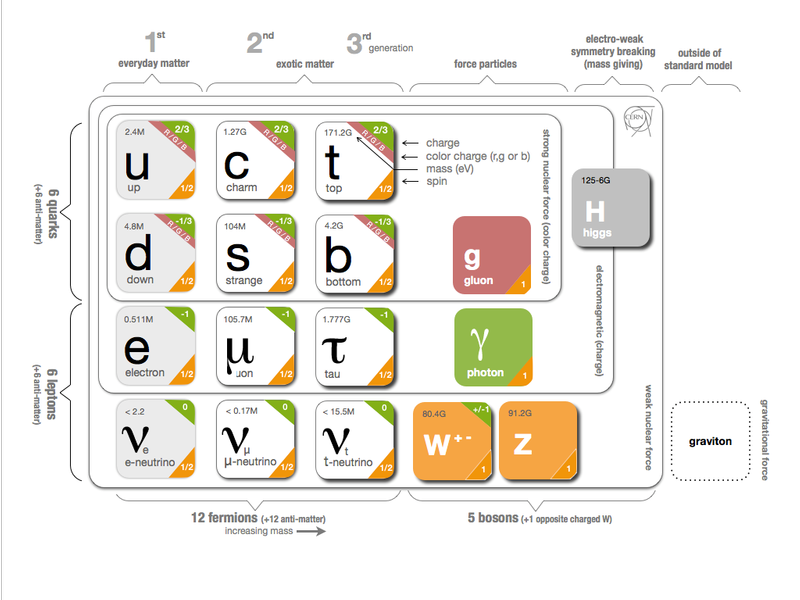
\includegraphics[width=\hsize]{figures/theory/particles.png}
  \caption{The particles of the Standard Model.} 
  \label{fig:sm_particles}
\end{figure}
\FloatBarrier

\begin{figure}[h!]
  \centering
  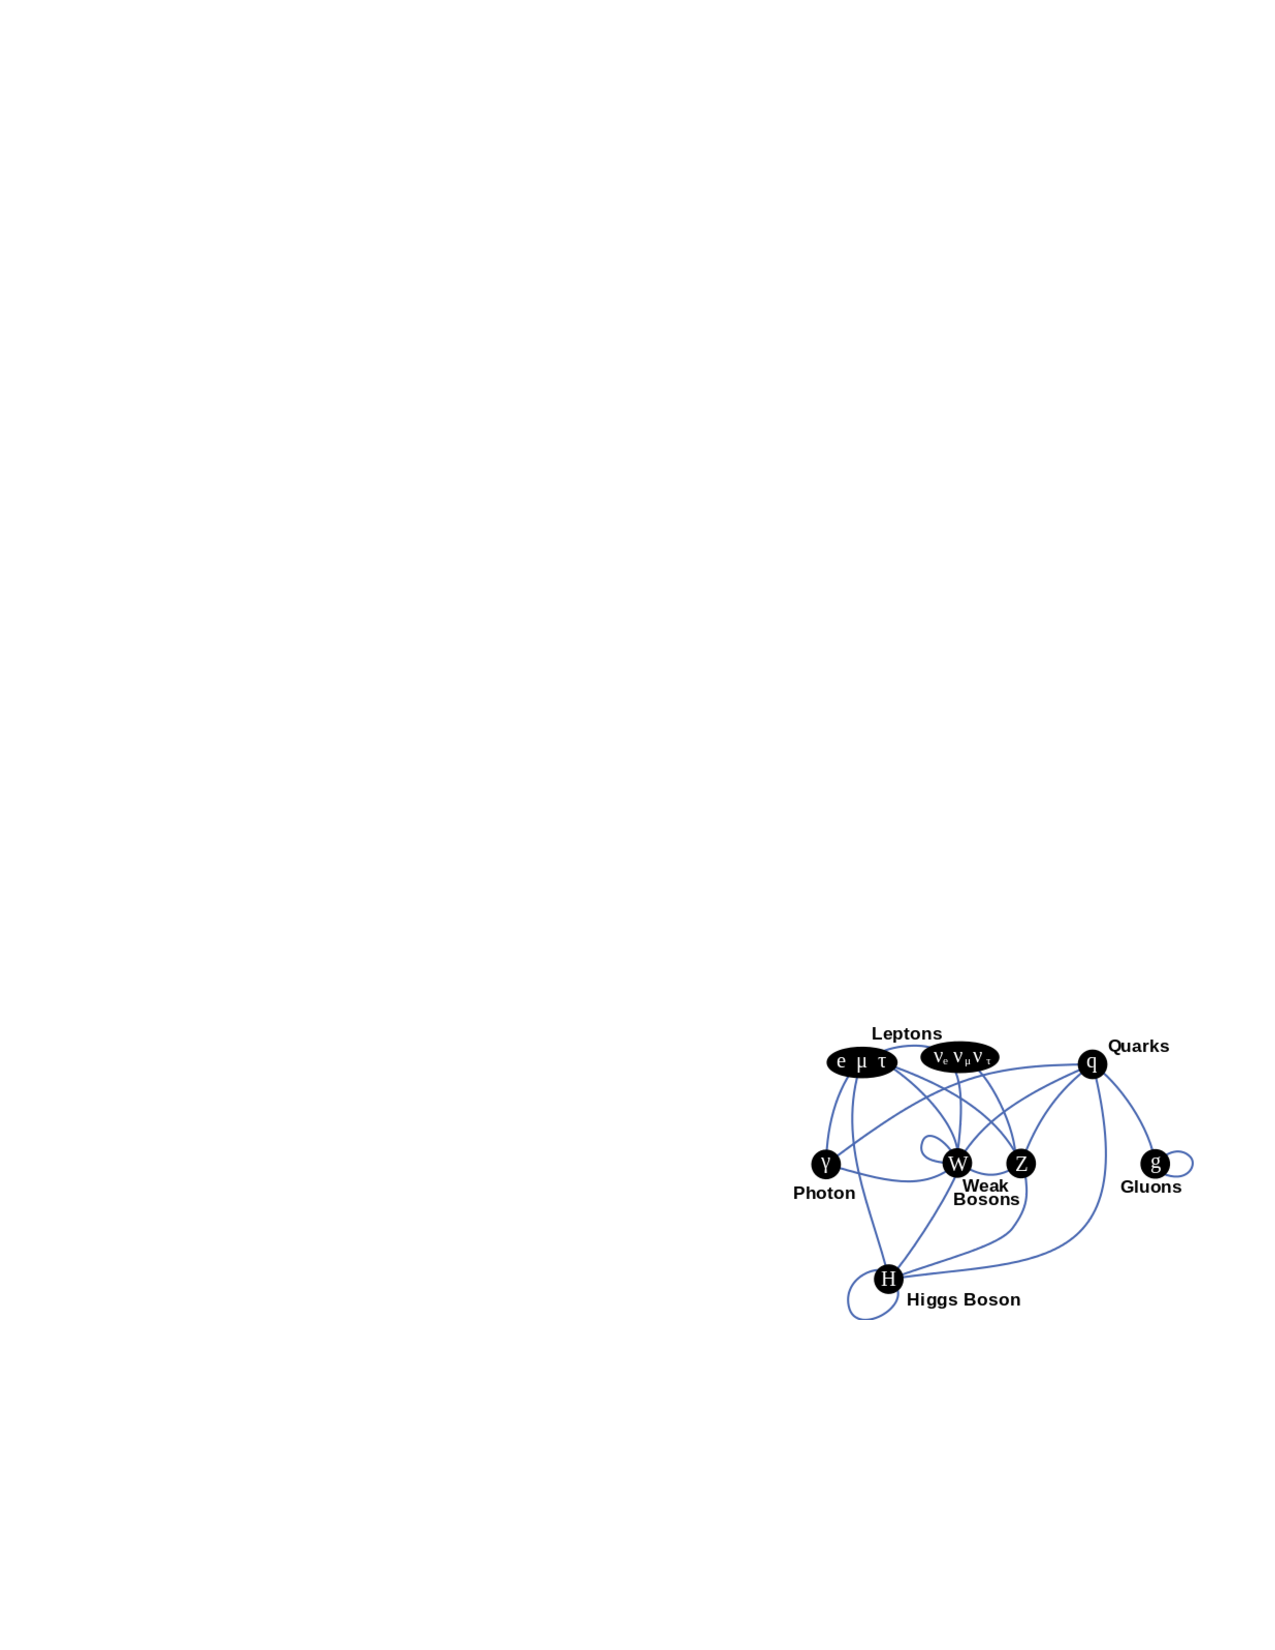
\includegraphics[width=\hsize]{figures/theory/particle_interactions.pdf}
  \caption{Summary of how Standard Model particles interact with other Standard Model particles.} 
  \label{fig:sm_particle_interactions}
\end{figure}
\FloatBarrier


Now we can understand the SM Lagrangian density as a Yang-Mills theory with the gauge group: $SU(3)_{C}\times SU(2)_{L} \times U(1)_{Y}$ with an additional $SU(2)$ complex scalar Higgs field doublet that will be discussed later.


\begin{flalign}\nonumber
\mathcal{L} _{SM} &= \underbrace{-\frac{1}{4}B_{\mu\nu}B^{\mu\nu}-\frac{1}{4}W^{a}_{\mu\nu}W^{a\mu\nu}-\frac{1}{4}G^{\alpha}_{\mu\nu}G^{\alpha\mu\nu}}_\text{Kinetic Energies and Self-Interactions of Gauge Bosons}&&\\\nonumber
&+\underbrace{\bar{L_{i}}\gamma^{\mu}(i\partial_{\mu}-\frac{1}{2}g_{1}Y_{iL}B_{\mu}-\frac{1}{2}g_{2}\sigma^{a}W_{\mu}^{a})L_{i}}_\text{Kinetic Energies and EW Interactions of Left-handed Fermions}&&\\\nonumber
&+\underbrace{\bar{R_{i}}\gamma^{\mu}(i\partial_{\mu}-\frac{1}{2}g_{1}Y_{iR}B_{\mu})R_{i}}_\text{Kinetic Energies and EW Interactions of Right-Handed Fermions}&&\\\nonumber
&+\underbrace{\frac{ig_{3}}{2}\bar{Q_{j}}\gamma^{\mu}\lambda^{\alpha}G^{\alpha}_{\mu}Q_{j}}_\text{Strong Interactions between Quarks and Gluons}&&\\\nonumber
&+\underbrace{\frac{1}{2}|(i\partial_{\mu}-\frac{1}{2}g_{1}B_{\mu}-\frac{1}{2}g_{2}\sigma^{a}W_{\mu}^{a})\Phi|^{2} - V(\Phi)}_\text{Electroweak Boson Masses and Higgs Couplings}&&\\\nonumber
&-(\underbrace{y^{d}_{kl}\bar{L_{k}}\Phi R_{l}+y^{u}_{kl}\bar{R_{k}}\widetilde{\Phi}L_{l}+h.c.)}_\text{Fermion Mass terms and Higgs Couplings}&&\\\nonumber
\end{flalign}

Here several abstract spaces are being spanned:
\begin{itemize}
\item[--]a spans the three $SU(2)_{L}$ gauge fields with generators expanded in Pauli matrics, $T^{\alpha}=\frac{1}{2}\sigma^{a}$
\item[--]$\alpha$ spans the eight $SU(3)_{C}$ gauge fields, with generators expanded in Gell-Mann matrices, $\tau^{\alpha}=\frac{1}{2}\lambda^{\alpha}$
\item[--]L/R represent left and right projections of Dirac fermion fields. The Strong interaction is not chiral, so Q = L+R
\item[--]$\mu$ and $\nu$ are four-vector indices
\item[--]i, j, k are summed over the three generations of SM particles. 
\end{itemize}

\section{Higgs Mechanism}
The SM Lagrangian without the addition of a Higgs field does not allow for gauge boson and fermion mass terms: $\frac{1}{2}m_{A}^{2}A_{\mu}A_{\mu}$ and $m(\bar{\psi}\psi)$,  as these terms are not gauge invariant. By introducing the Higgs field, mass terms for these particles may be included in a gauge invariant way. This field is a complex doublet with a potential $V(\Phi)$:

\begin{equation}
\Psi = \begin{pmatrix} \Phi^{\dagger} \\ \Phi^{0} \end{pmatrix}
\end{equation}
\begin{equation}
V(\Phi)=\mu^{2}\Phi^{\dagger}\Phi + \lambda |\Phi^{\dagger}\Phi|^{2}
\end{equation}

The minima of this field occurs for $|\Phi|= \sqrt{\frac{\mu^{2}}{2\lambda}} \equiv \frac{v}{2}$. This yields degenerate minima, this symmetry is broken by choosing a specific minima (a.k.a. spontaneous symmetry breaking). By convention  $\Phi_{min} = \frac{1}{\sqrt{2}}\begin{pmatrix}0 \\ v \end{pmatrix}$ is chosen. This means the ground state of the Higgs field (Higgs vacuum) is non-zero, $\sqrt{\frac{-\mu^{2}}{\lambda}}$. The Higgs Field may now be expanded around this new ground state:

\begin{equation}
\Phi(x)=\frac{1}{\sqrt{2}}\begin{pmatrix} 0 \\ v+h(x)\end{pmatrix}
\end{equation}

This non-zero Higgs vacuum now generates mass terms for the gauge bosons from the following term in the Lagrangian:

\begin{equation}
|(-\frac{1}{2}g_{1}B_{\mu}-\frac{1}{2}g_{2}\sigma^{a}W_{\mu}^{a})\Phi|^{2}=\frac{1}{2}m_{W}^{2}W_{\mu}^{+}W^{-\mu}+\frac{1}{2}m_{Z}^{2}Z_{\mu}Z^{\mu}
\end{equation}

where:
\begin{equation}
W^{\pm}_{\mu} \equiv \frac{1}{\sqrt{2}}(W^{1}_{\mu} \mp iW^{2}_{\mu})
\end{equation}
\begin{equation}
Z_{\mu} \equiv \frac{1}{\sqrt{g_{1}^{2}+g_{2}^{2}}}(g_{2}W^{2}_{\mu}-g_{1}B_{\mu})
\end{equation}
\begin{equation}
m_{W} = \frac{vg_{2}}{\sqrt{2}}
\end{equation}
\begin{equation}
m_{Z} = \frac{v}{\sqrt{2}}\sqrt{g_{1}^{2} + g_{2}^{2}}
\end{equation}

The Higgs field also generates a mass term for the Higgs boson and self-interactions for the Higgs boson. 
\section{Electroweak Theory}
$SU(2)_{L}$ generates $W^{\pm}, W^{0}$ gauge bosons, which would be massless if $SU(2)_{L}$ was a perfect symmetry. These bosons are massive as this symmetry is broken. The mass eigenstates, Z and $\gamma$ given by: 
\begin{equation}
\begin{pmatrix} Z_{\mu} \\ A_{\mu} \end{pmatrix} = \begin{pmatrix} \cos \theta_{W} & -\sin \theta_{W} \\ \sin \theta_{W} & \cos \theta_{W} \end{pmatrix} \begin{pmatrix} W^{3}_{\mu} \\ B_{\mu} \end{pmatrix}
\end{equation} 

Here $\theta_{W}$ is the Weinberg angle given by: 
\begin{equation}
\cos\theta_{W}=\frac{g_{2}}{\sqrt{g_{1}^{2}+g_{2}^{2}}} = \frac{m_{W}}{m_{Z}}
\end{equation}
\section{Quantum ChromoDynamics}
As mentioned earlier the Strong Force, which binds the proton together, is mediated by gluons. Quantum Chromodynamics is the QFT which describes the interactions of quarks and gluons via $SU(3)_C$ symmetry. QCD contains features not present in Electroweak Interactions due to $SU(3)_C$ generators not commuting (a.k.a. $SU(3)_C$ is a non-abelian group) and the number of quark flavors ($n_{f}$). For example, in QCD there is color confinement and asymptotic freedom due to the structure constants being non-zero. Requiring $SU(3)_C$ local gauge invariance implies:

\begin{equation}
\psi(x) \rightarrow \psi(x)^{'} = \exp[ig_{S}\alpha(x)\cdot\hat{T}]\psi(x)
\end{equation}

where $\alpha(x)$ is the local phase function, $g_{S}$ is the strong coupling constant, and $\hat{T}$ are the eight generators of $SU(3)$ (note $\hat{T^{a}}=\frac{1}{2}\lambda^{a} a$, where $\lambda^{a}$ are the Gell-Mann matrices). As the Gell-Mann matrices are 3x3, this means $\psi$ has three degrees of freedom under these $SU(3)$ rotations. So we represent $\psi$ under $SU(3)$ rotations as:

\begin{equation}
\psi = \begin{pmatrix} \psi_{red} \\ \psi_{green} \\ \psi_{blue}\end{pmatrix}
\end{equation}

Consequently, particle fields transforming under $SU(3)$ rotations have three components which physicists describe as color components (red, green, and blue). A particle's corresponding antiparticle has the corresponding anticolor. This color is the "charge" of QCD and is conserved under $SU(3)$ rotations. Combining colors, color neutral states (e.g. red and antired, or red, green and blue) may be created.
For the free Dirac Lagrangian to remain invariant under $SU(3)$ transformations, we must again postulate a boson field that modifies the derivative. The gluon field tensor is given by ($\alpha=1,...,8)$:

\begin{equation}
G_{\mu\nu}^{k}  = \partial^{\mu}G^{\nu}_{\alpha}-\partial^{\nu}G^{\mu}_{\alpha}-g_{S}f^{\alpha\beta\gamma}G^{\mu}_{\beta}G^{\nu}_{\gamma}
\end{equation}

Here $f^{\alpha\beta\gamma}$ are the structure constants of $SU(3)$. Combining all this gives the QCD Lagrangian:

\begin{equation}
\mathcal{L}_{QCD} = \bar{\psi_{qi}}i\gamma^{\mu} (D_{\mu})_{ij}\psi^{qj} - m\bar{\psi^{qi}}\psi_{qi} - \frac{1}{4}G^{\alpha}_{\mu\nu}G^{\alpha\mu\nu} 
\end{equation}

Here i are the color indicies, and q are the quark flavors. It is important to note that quarks transform under the fundamental representation of $SU(3)$, while gluons transform under the adjoint representation. This means quarks carry a single color charge (red, green, blue, antired, antigreen, antiblue) and gluons carry a color and anticolor charge. 

Figure \ref{fig:QCDinteractions} shows the three dominant QCD interactions. Sincle gluons carry color charge, they interact with one another. This does not occur in QED, as photons do not have electric charge and therefore do not interact with each other. In QED, a bare electron's effective charge is largest closest to the electron and decreases as a function of distance. This is because the QED vacuum fills with particle antiparticle pairs spontaneously, which screen the charge of the bare electron. The larger the distance from the electron, the smaller the effective charge and therefore the weaker the force. 

\begin{figure}[h!]
  \centering
  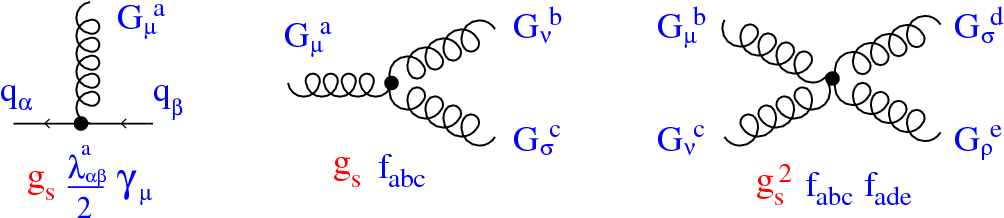
\includegraphics[width=\hsize]{figures/Theory/QCD_vertices.png}
  \caption{This figure shows the three dominant QCD interactions \cite{pich}}f. 
  \label{fig:QCDinteractions}
\end{figure}
\FloatBarrier


As the distance from a quark increases it's effective color charge increases due to the vacuum polarization in QCD. Color charge grows as the distance from the source increases (a.k.a. color is anti-screened in QCD).  In this way, strong interactions become stronger at large distances (low momenta interactions).  At small distances (large momenta interactions) strong interactions are significantly weaker and considered nearly free. This effect of referred to as asymptotic freedom. At large distances, a quark's effective charge is large and the strong force is more significant. This force becomes so strong that quarks form colorless bound states instead of remaining free particles. This effect is known as color confinement. This running of all SM fields is shown in Figure ~\ref{fig:sm_couplings}. 

\begin{figure}[h!]
  \centering
  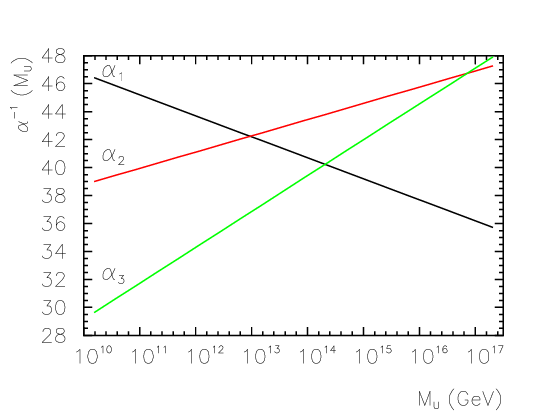
\includegraphics[width=\hsize]{figures/Theory/runningcouplings.png}
  \caption{Strength of the $U(1)$, $SU(2)$, and $SU(3)$ gauge couplings as a function of the energy scale of the interaction (Q). From Ref. \cite{runningcouplings}}. 
  \label{fig:sm_couplings}
\end{figure}
\FloatBarrier


Commonly the change in a particle's effective charge under a given force is quantified with  $\beta(r) \equiv \frac{-de(r)}{d\ln r}$, where e(r) is the effective charge of a given particle under a force. In QED this function is positive but in QCD this function is negative leading to confinement and asymptotic freedom. Moreover, one can calculate how the coupling ($\alpha$) of a force varies with energies. More deeply this amounts to incorporating renormalization and vacuum polarization in the boson propagators. For QCD this is:

\begin{equation}
\alpha_{S}(Q^{2}) = \frac{ \alpha_{s}(\mu^{2}) } { 1+ \frac{ \alpha_{s}( \mu^{2} ) } { 12\pi } ( 33-2n_{f} ) ln( Q^{2}/\mu^{2})}  
\end{equation}


where $Q$ is the momentum of the the force is probed at, $\mu^{2}$ is the renormalization scale, $n_{f}$ is the number of quark flavors. There are six quark flavors in SM QCD, making $33-2n_{f} > 0$. This factor being positive and the $ln(Q^{2}/\mu^{2})$  being in the denominator means that as $Q^{2}$ increases $\alpha_{s}$ decreases. So for large $Q^{2}$, $\alpha_{s}$ is small and SM QCD is asymptotically free, while for small $Q^{2}$, $\alpha_{s}$ is large and SM QCD is confined, as mentioned earlier. 

As stated previously, quarks and gluons have not been observed in isolation. Instead they form bound colorless states. Hadronization is the process by which quarks and gluons form hadrons. The process of hadronization is still an active area of research. One qualitative description is show in Figure \ref{fig:colorstring}. In this figure, as two quarks separate the color field between them is restricted to a tube with energy density of ~1 GeV/fm. As they separate further, the energy in the color field increases, until there is enough energy to produce $q\bar{q}$ pairs, which breaks the color field. This process repeats until quarks and antiquarks have low enough energy to form colorless hadrons. The resulting spray of hadrons is called a jet.

Since quarks and gluons carry different color charges, their respective jets have different properties. As quarks carry only a single color charge (vs. gluons which have color and anticolor charge), so their jets have less constituent particles. More precisely, the Altarelli-Parisi splitting functions ~\cite{altarelli} contain a factor $C_{A}$ for gluon radiation off a gluon and $C_{F}$ for gluon radiation off a quark ($C_{A}/C_{F} = 9/4$). These color factors are the prefactor in the Feynman diagrams for these processes ~\cite{colorfactor}, which leads to gluon jets having more constituents and therefore more tracks than quark jets. Gluon jets also tend to have a larger radius with lower momentum constituents than quarks. There are many novel techniques to distinguish quarks from gluons. For this study the number of charged particles will be focused on.  

\begin{figure}[h!]
  \centering
  \includegraphics[width=\hsize]{figures/Theory/color_string.pdf}
  \caption{A cartoon of string breaking: the QCD string spanned between quark Q and antiquark $\bar{Q}$ breaks due to $q\bar{q}$ creation \cite{colorstring}}.
  \label{fig:colorstring}
\end{figure}
\FloatBarrier

\chapter{Standard Model Successes and Limitations}
The Standard Model has accurately described most of the underlying principles of nature. It has predicted cross sections for strong and electroweak processes that span over ten orders of magnitude correctly, as shown in Figure \ref{fig:SM cross sections}, and contains no known logical inconsistencies. Despite the strength and reality of the Standard Model, it still fails to describe some important aspects of reality and suffers from aesthetic issues. 
To date, dark matter and dark energy comprise $\sim 95\%$ of the universe, but the SM offers no explanation of their nature. Additionally, neutrinos are known to have mass, but the SM offers no mass generation mechanism for left-handed neutrinos without right-handed neutrinos (which do not exist). There are other mechanisms for introducing massive neutrinos in the SM, but these mechanisms create hierarchy problems. 

Possibly the most significant aesthetic issue is the hierarchy between the electroweak and Planck scales. The electroweak scale is the scale of electroweak symmetry breaking. The Planck scale is the scale where the gravitational force is comparable in strength to the other forces. The Planck scale is where the SM breaks down, as there is not an experimentally verified theory of quantum gravity, and at this scale gravity cannot be ignored (like it can at the electro-weak scale). These scales differ by $\sim30$ orders of magnitude. Understanding the difference in these energy scales may help explain the weakness of gravity at electroweak scales, and possibly a QFT for gravity. (NB: This hierarchy can also be framed in terms of the corrections to the Higgs mass, which depend on the UV cutoff scale - where the SM is suppose to break, which is taken at the Planck scale. This leads the quantum corrections to the Higgs mass that would force the Higgs mass to $\sim 10^{18}$ TeV.)

These stark contrasts in scales may indicate that a more fundamental theory exists. It is hoped that such a theory would explain and motivate some of the ad-hoc features of the SM. In particular, the SM does not offer an explanation for the values of the 19 SM parameters (6 quark masses, 3 charged lepton masses, 3 gauge couplings, Higgs parameters ($\mu^{2}$, $\lambda$)) and the structure of the fermion representations.


\begin{figure}[h!]
  \centering
  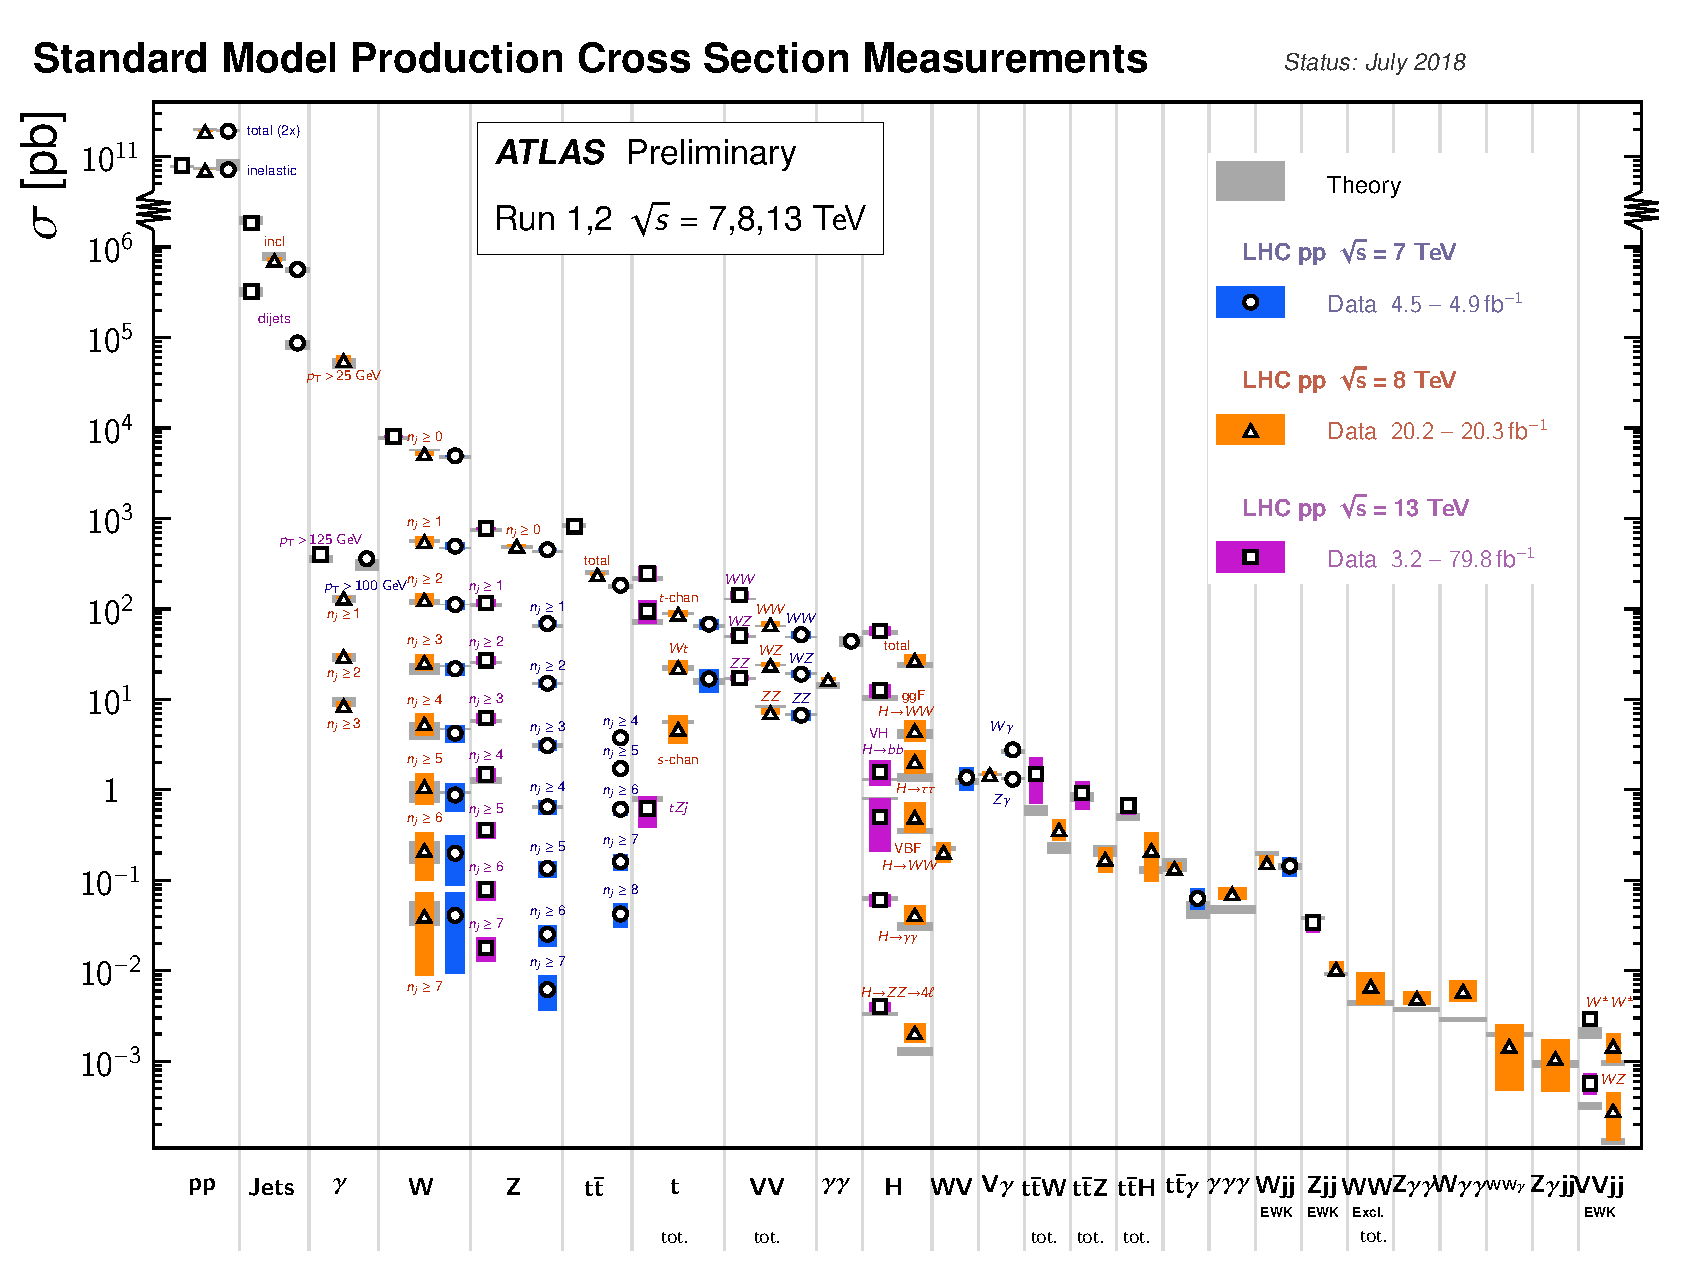
\includegraphics[width=\hsize]{figures/Theory/SM_xs.pdf}
  \caption{A comparison of cross section measurements at $\sqrt{s}=7,8,13$ TeV from ATLAS compared to theoretical measurements. From Ref. \cite{SM_XS_Comparison}}. 
  \label{fig:SM cross sections}
\end{figure}
\FloatBarrier


\chapter{New Physics Models with Diboson Resonances}
\label{BSM chapter}

\section{Randall Sundrum Bulk Model}
%Top down approach (solve gravity problem)
The electroweak-planck hierarchy may be explained by the existence of extra dimensions, like the 5D Randall Sundrum Bulk Model (\cite{rs2},\cite{rs1}). In this model, there is one extra warped spatial dimension, y, with a metric:
\begin{equation}
ds^{2}=e^{-2k|y|}\eta_{\mu\nu}dx^{\mu}dx^{\nu}+dy^{2} 
\end{equation}
where $e^{-k|y|}$ is the warp factor of the extra dimension, which is compactified on a $S^{1}/Z_{2}$ orbifold (a.k.a. a circle where $y \rightarrow -y$). This can be visualized as every point in space time having a line extending from it a distance L, representing this fifth dimension. At the end of this line is the Planck brane. This fourth spatial dimension separates two 4-D branes: Planck brane and TeV brane. We live on the TeV brane, as shown in Figure ~\ref{fig:RS_cartoon}. The Higgs field (and to a lesser degree the top quark and graviton fields) is localized near the TeV Brane, while the light fermion fields are localized more near the Planck brane. Fundamental parameters are set on the Planck brane. The warp factor may be scaled away from all dimensionless SM terms by field redefinitions. However, the only dimensionful parameter, $m_{H}^{2}=v^{2}$ is rescaled by $\tilde{v}\sim e^{-kL}M_{Pl}\sim 1$TeV for $kL\sim 35$, explaining why gravity is so weak on the TeV brane. Also, by localizing the light fermion fields near the Planck brane and top and graviton fields near the TeV brane, the light quarks will have smaller masses. 

The two free parameters of this theory are $M_{PL}$ and $k$. Based on this RS Bulk model, all SM particles should have Kaluza-Klein (KK) excitations. In particular, the graviton would have KK excitations that prefer to decay to WW or ZZ, which is why this analysis searches for RS Gravitons. 


\begin{figure}[h!]
  \centering
  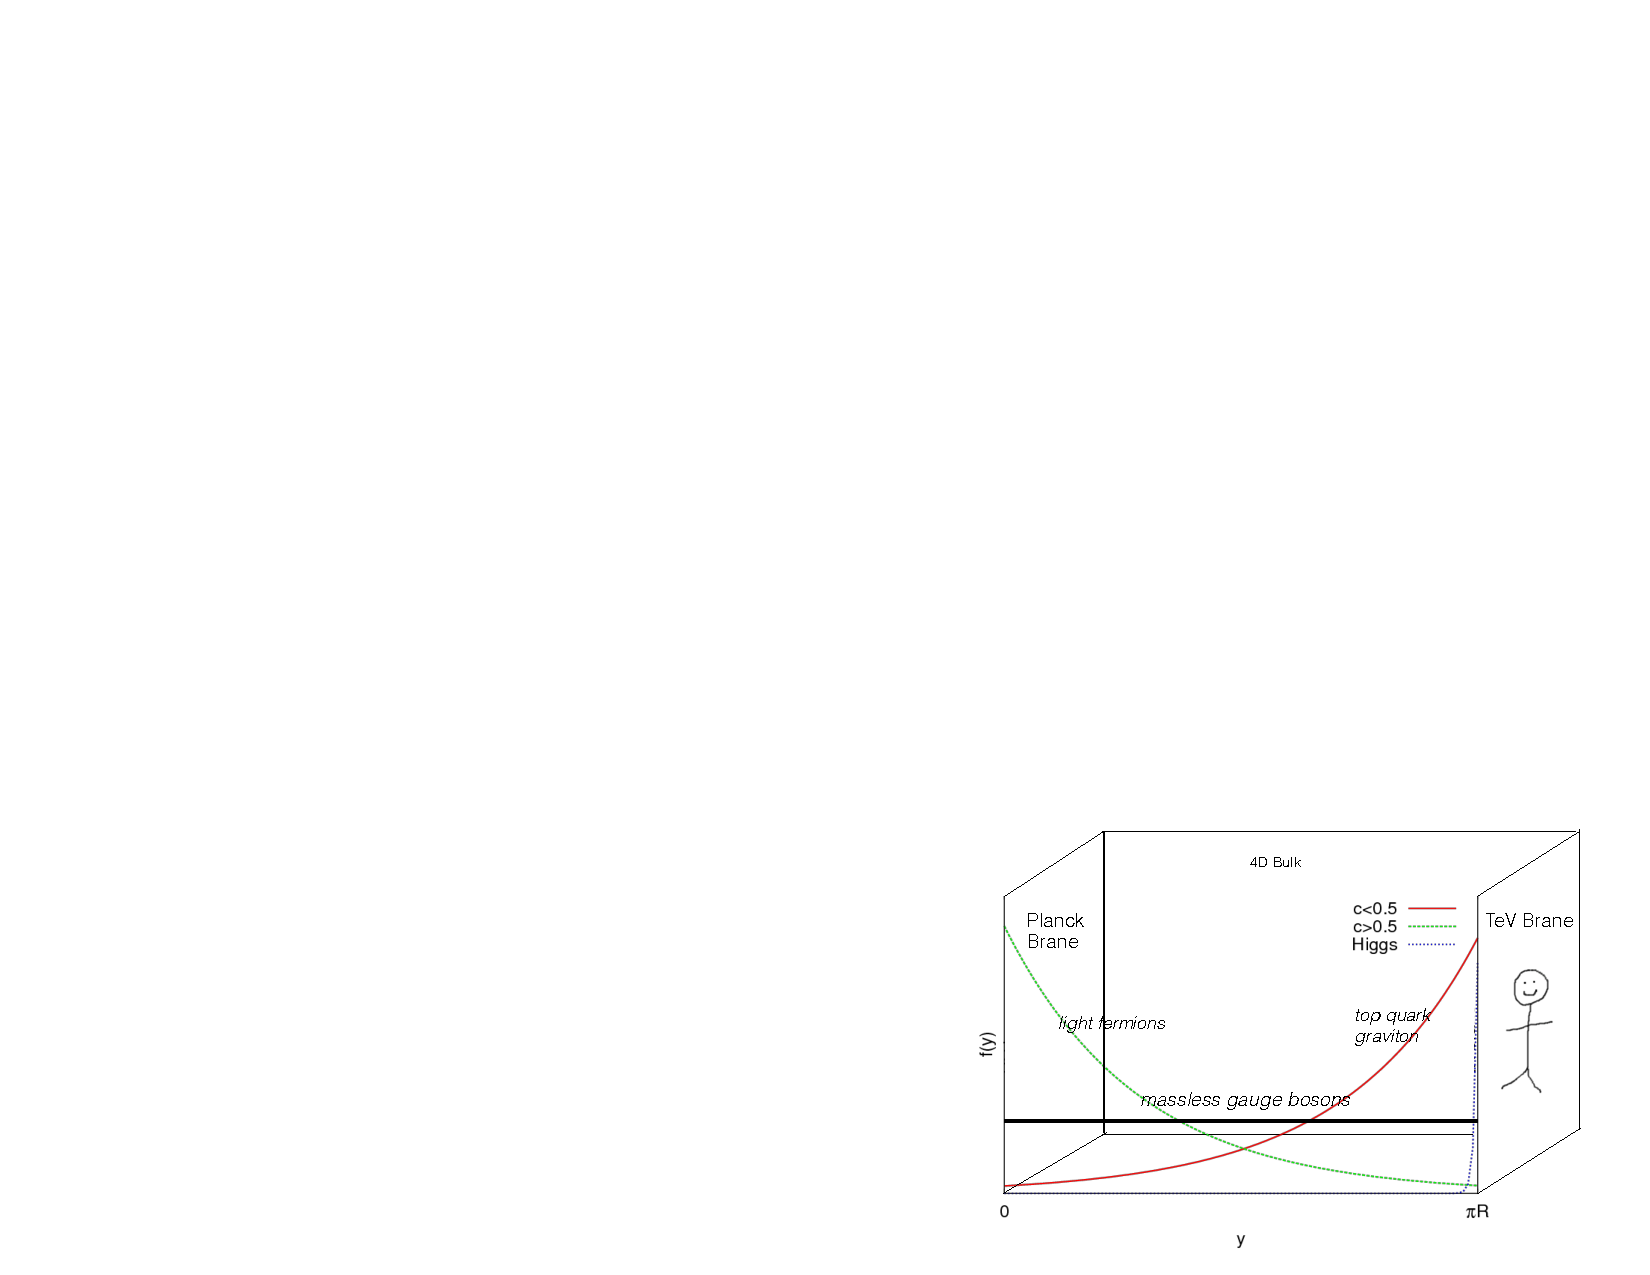
\includegraphics[width=\hsize]{figures/Theory/RS_cartoon.pdf}
  \caption{Cartoon of RS Bulk Model}. 
  \label{fig:RS_cartoon}
\end{figure}
\FloatBarrier

\begin{comment}
\section{Extended Scalar Sector}
%tries to solve physics problem but also somewhat ad-hoc (just a parameterization)
A further striking asymmetry of the SM is the simplicity of the scalar sector in comparison to the boson and fermion sectors. To date, the scalar sector has only one member, the Higgs boson. Therefore, it is natural to posit an extension to the scalar sector. From a theoretical standpoint this could also help generate baryon asymmetry through additional sources of CP violation. This analysis searches for a simple extension to the scalar sector as proposed in Ref. \cite{scalarsinglet}. The extended scalar sector includes a real Higgs singlet (S) and complex $SU(2)_{L}$ doublet ($\Phi$) (the SM Higgs), where mass eigenstates are mixtures of the fields. S has a vev of $v$ and $\Phi$ has a vev of $x$. This then gives a Lagrangian of:

\begin{equation}
\mathcal{L}\supset (D^{\mu}\Phi)^{\dag}D_{\mu}\Phi + \partial^{\mu}S\partial_{\mu}S - m^{2}\Phi^{\dag}\Phi-\mu^{2}S^{2} + \lambda_{1}(\Phi^{\dag}\Phi)^{2} + \lambda_{2}S^{4}+\lambda_{3}\Phi^{\dag}\Phi S^{2}
\end{equation}


The mass eigenstates of the scalar sector are then mixtures of $S$ and $\Phi$ and the free parameters of the theory are $m_{H}$, $\sin\alpha$, and $tan\beta=v/x$. The fields are then given by:

\begin{equation}
\Phi \equiv \begin{pmatrix} 0 \\ \frac{\tilde{h}+v}{\sqrt{2}} \end{pmatrix}
\end{equation}
\begin{equation}
S \equiv \frac{h'+x}{\sqrt{2}}
\end{equation}

Diagonalizing the mass matrix leads to the mass eigenstates h (discovered Higgs boson) and H (the physical particles):

\begin{equation}
\begin{pmatrix} h \\ H \end{pmatrix} = \begin{pmatrix} \cos\alpha &-\sin\alpha \\ \sin\alpha & \cos\alpha \end{pmatrix}
\end{equation}
This suppressed h and H production and SM H couplings:

\begin{equation}
BR_{H \rightarrow SM}=\sin^{2}\alpha \times \frac{\Gamma_{SM, H \rightarrow SM}}{\Gamma_{tot}}
\end{equation}
Moreover, in the case that $m_{H} > m_{h}$, $H\rightarrow hh$ is possible. This further suppresses $H \rightarrow VV/ff$. This search is most sensitive to $H \rightarrow WW$.
\end{comment}

\section{Simple Standard Model Extensions}
\label{HVT chapter}
The RS Bulk model is motivated by resolving SM hierarchies, but it does not address all of the other SM issues. There are many other interesting and well motivated new physics frameworks that address these issues, but there is a lack of completely predictive models, due to model flexibility (free parameters). It is difficult for experimentalists to know which theories to search for in data. Therefore, developing a model-independent resonance search that can be reinterperted in the context of a given BSM theory is ideal.

This search is sensitive to the resonance mass and its interactions, but not all of a given BSM model's parameters. Therefore, the BSM Lagrangian may be reduced to only retain this information (mass parameters and couplings) following the procedure in \cite{hvt}.
In this simplified approach, the new resonance searched for is represented as an additional heavy vector triplet (HVT), which is a real vector field in the adjoint representation of $SU(2)_{L}$ with vanishing hypercharge. This results in one neutral and two charged bosons, defined as:

\begin{equation}
V^{\pm}=\frac{V^{1}_{\mu}\mp iV^{2}_{\mu}}{\sqrt{2}}
\end{equation}
\begin{equation}
V^{0}_{\mu}=V^{3}_{\mu}
\end{equation}

The SM Lagrangian is then augmented with the additional terms:
\begin{equation}
\label{hvt_lagrangian}
\mathcal{L}\supset -\frac{1}{4}D_{[\mu}V^{a}_{\nu]}D^{[\mu}V^{\mu]a} + \frac{m_{V}^{2}}{2}V^{a}_{\mu}V^{a\mu} + ig_{V}c_{H}V^{a}_{\mu}H^{\dag}\tau^{a}\overset\leftrightarrow{D^{\mu}}H+\frac{g^{2}}{g_{V}}c_{F}V^{a}_{\mu}J_{F}^{\mu a}
\end{equation}


In order the terms represent: the kinetic, $V$ mass, Higgs-$V$ interaction, and $V$-left-handed fermion interaction terms. The $g_{V}$ coupling factor determines the coupling of the new resonance to left-handed fermions and the Higgs boson. 

As benchmark models, this search considers resonances from extended gauge symmetry (EGM) and composite Higgs models as discussed in \cite{hvt} . The EGM model predicts weakly coupled resonances, where $g_{V} = 1$, referred to later as Model A. The composite Higgs Model is a strongly coupled model, where $g_{V}=3$, and later referred to as Model B. 
As shown in Eq. \ref{hvt_lagrangian}, the coupling of these resonances to fermions scales as $g_{f} = g^{2}c_{F}/g_{V}$, where g is the SM $SU(2)_{L}$ gauge coupling and $c_{F}$ is a free parameter. This then means that for Model B the coupling to fermions is suppressed relative to Model A, leading to a smaller DY production rate and branching ratio (BR) to fermionic final states. The coupling of $V$ to SM bosons scales as $g_{H}=g_{V}c_{H}$, where $c_{H}$ is a free parameter on the order of one for Model A and B. Consequently Model A resonances have a smaller the BR to gauge bosons than Model B. For the $pp$ collision data used, Model A predicts larger production cross sections decaying to leptons and fermions than Model B which decays primarily to gauge bosons.

Model A and B vectors are produced via quark-anti-quark annihilation and the more rare vector-boson-fusion is considered by setting $g_{H} = 1$ and $g_{F}=0$. Both production modes are probed in this resonance search. 

In summary, $V$ couples most strongly to left-handed fermions and $VV$ dependent on $g_{V}$. 


\part {Experimental Setup}
\label{ch:detector}
\chapter{LHC}
The Large Hadron Collider (LHC) is the highest-energy particle collider in the world. It was designed to expand the frontier of high energy particle collisions in energy and luminosity. This enables LHC experiments to test the Standard Model and search for new physics at higher energies than tested with previous colliders. Collisions at higher energies not only produce more massive particles but also more weakly interacting particles. Fig ~\ref{fig:xs_scaling} shows production cross sections for various processes at hadron colliders. The rate for electroweak physics processes including $W$ and $Z$ scale with the center-of-momentum energy, $\sqrt{s}$.

The LHC consists of a 26.7 km (17 miles) ring, approximately 100 m underground, outside Geneva, Switzerland. Counter-circulating proton (and occasionally heavy ions) beams collide inside four experiments along the beam line: ATLAS, CMS, LHCb, ALICE. ATLAS and CMS are general purpose detectors designed to explore the high energy frontier. LHCb is designed to study the physics of $b$-quarks. ALICE specializes in studying heavy ion collisions. 


\begin{figure}[h!]
  \centering
  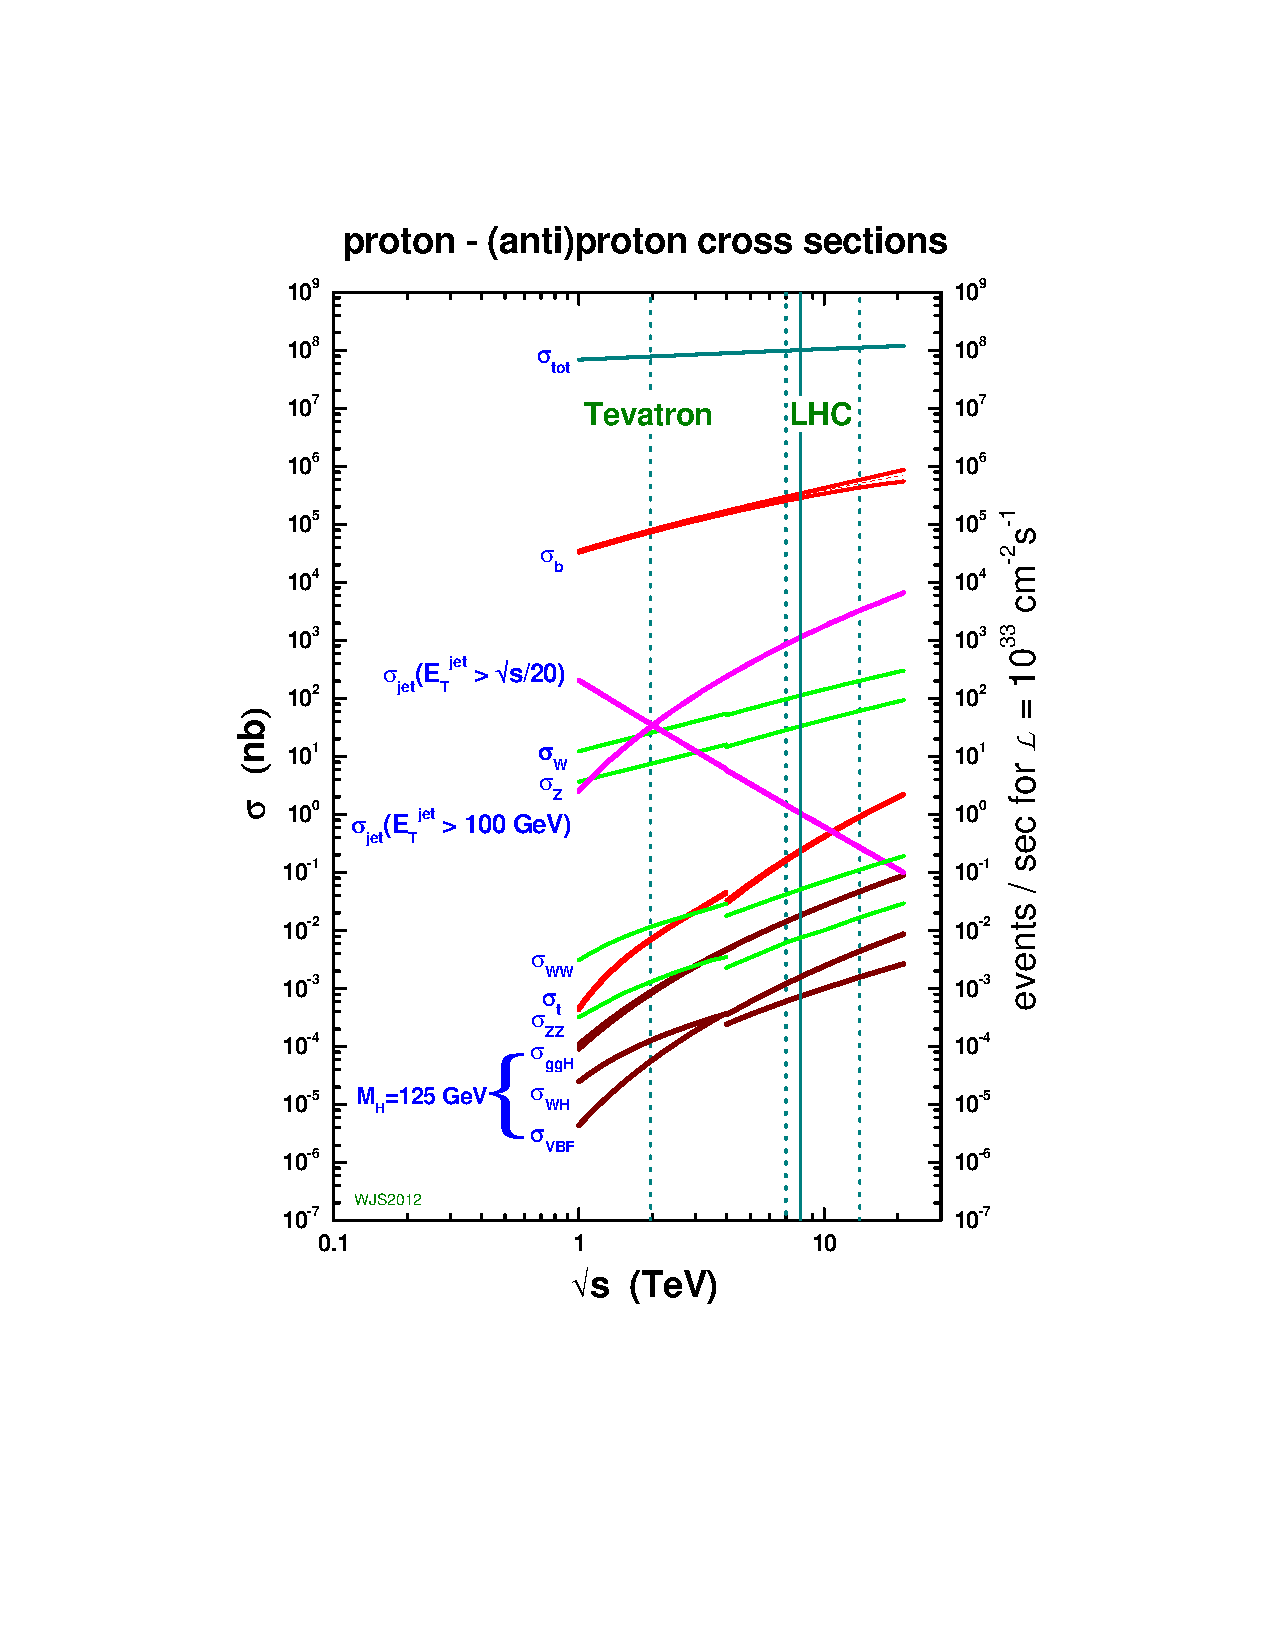
\includegraphics[width=\hsize]{figures/Detector/xs_scaling.pdf}
  \caption{Scaling of various SM cross sections with $\sqrt{s}$.}. 
  \label{fig:xs_scaling}
\end{figure}
\FloatBarrier


The first proton beams circulated in September, 2008. Nine days later an electrical fault lead to mechanical damage and liquid helium leaks in the collider. This incident delayed further operation until November 2009, when the LHC became the world's highest energy particle collider, at 1.18TeV per beam. This first operational run continued until 2013, reaching 7 and 8 TeV collision energies. During this run a particle with properties consistent with the Standard Model Higgs boson was discovered. The next run began after a two year shutdown after upgrades to the LHC and experiments. This run lasted from 2013 to 2018 reaching 13 TeV collision energies. This analysis uses data from the second operational run. 
\section{LHC Layout and Design}
The layout of the LHC is shown in Figure ~\ref{fig:lhc_layout}. The red and blue lines in the figure represent the counter-circulating proton beams. The LHC is divided into eight octants.  Octant 4 contains the RF cavities that accelerate the protons and octant 6 contains the beam dump system. Octants 3 and 7 house the collimation systems for beam cleaning. The beams collide inside the four aforementioned experiments. Each octant contains a curved and straight section. The LHC magnets are built with NBTi superconductors cooled with super-fluid Helium to 2K, creating a 8.3T magnetic field to bend the proton beams.


\begin{figure}[h!]
  \centering
  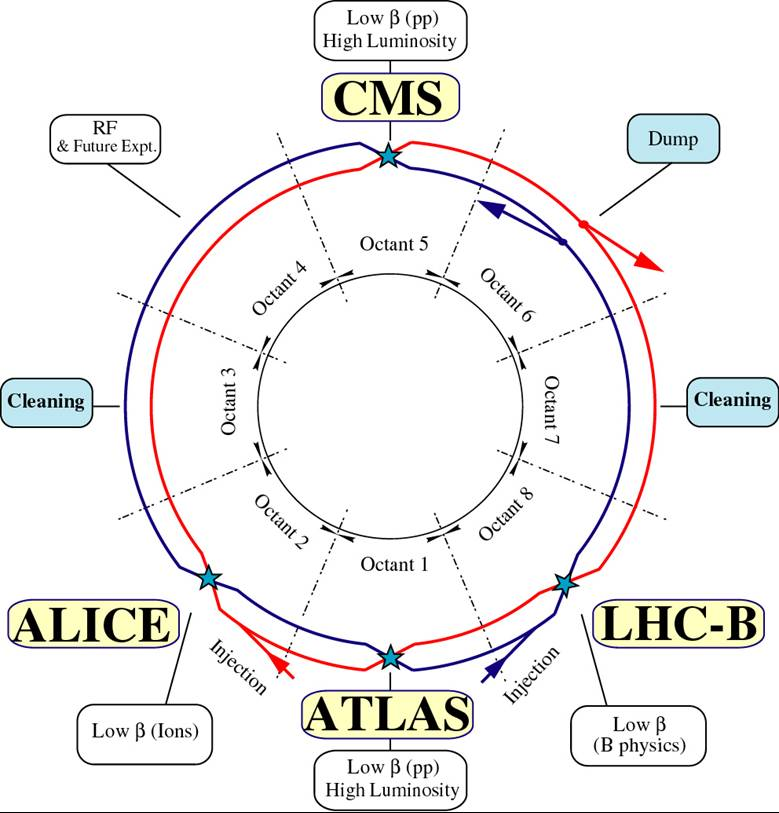
\includegraphics[width=\hsize]{figures/Detector/lhc.jpg}
  \caption{The layout of the LHC and the four detectors along the beam line (ATLAS, LHCb, ALICE, CMS).}. 
  \label{fig:lhc_layout}
\end{figure}
\FloatBarrier


Four sequential particle accelerators are used to accelerate protons from rest as shown in Figure \ref{fig:lhc_accel}. First, Hydrogen gas is ionized to produce protons which are then accelerated to 50 MeV using Linac 2, a linear accelerator. The resulting proton beam is then passed to three circular particle accelerators: Proton Synchrotron Booster, Proton Synchrotron, and Super Proton Synchrotron (SPS), accelerating protons to 1.4, 25, and 450 GeV, respectively. Once the protons exit the SPS, they are injected into the LHC at octant 2 and 8. Each proton bunch contains $\sim 10^{11}$ protons. The spacing between bunches is 25 ns, which means each beam contains 3564 bunches. However, some bunches are left empty due to injection and safety requirements, yielding 2808 bunches per beam. Once the proton beams are injected they are accelerated to 13 TeV. 


\begin{figure}[htbp]
  \centering
  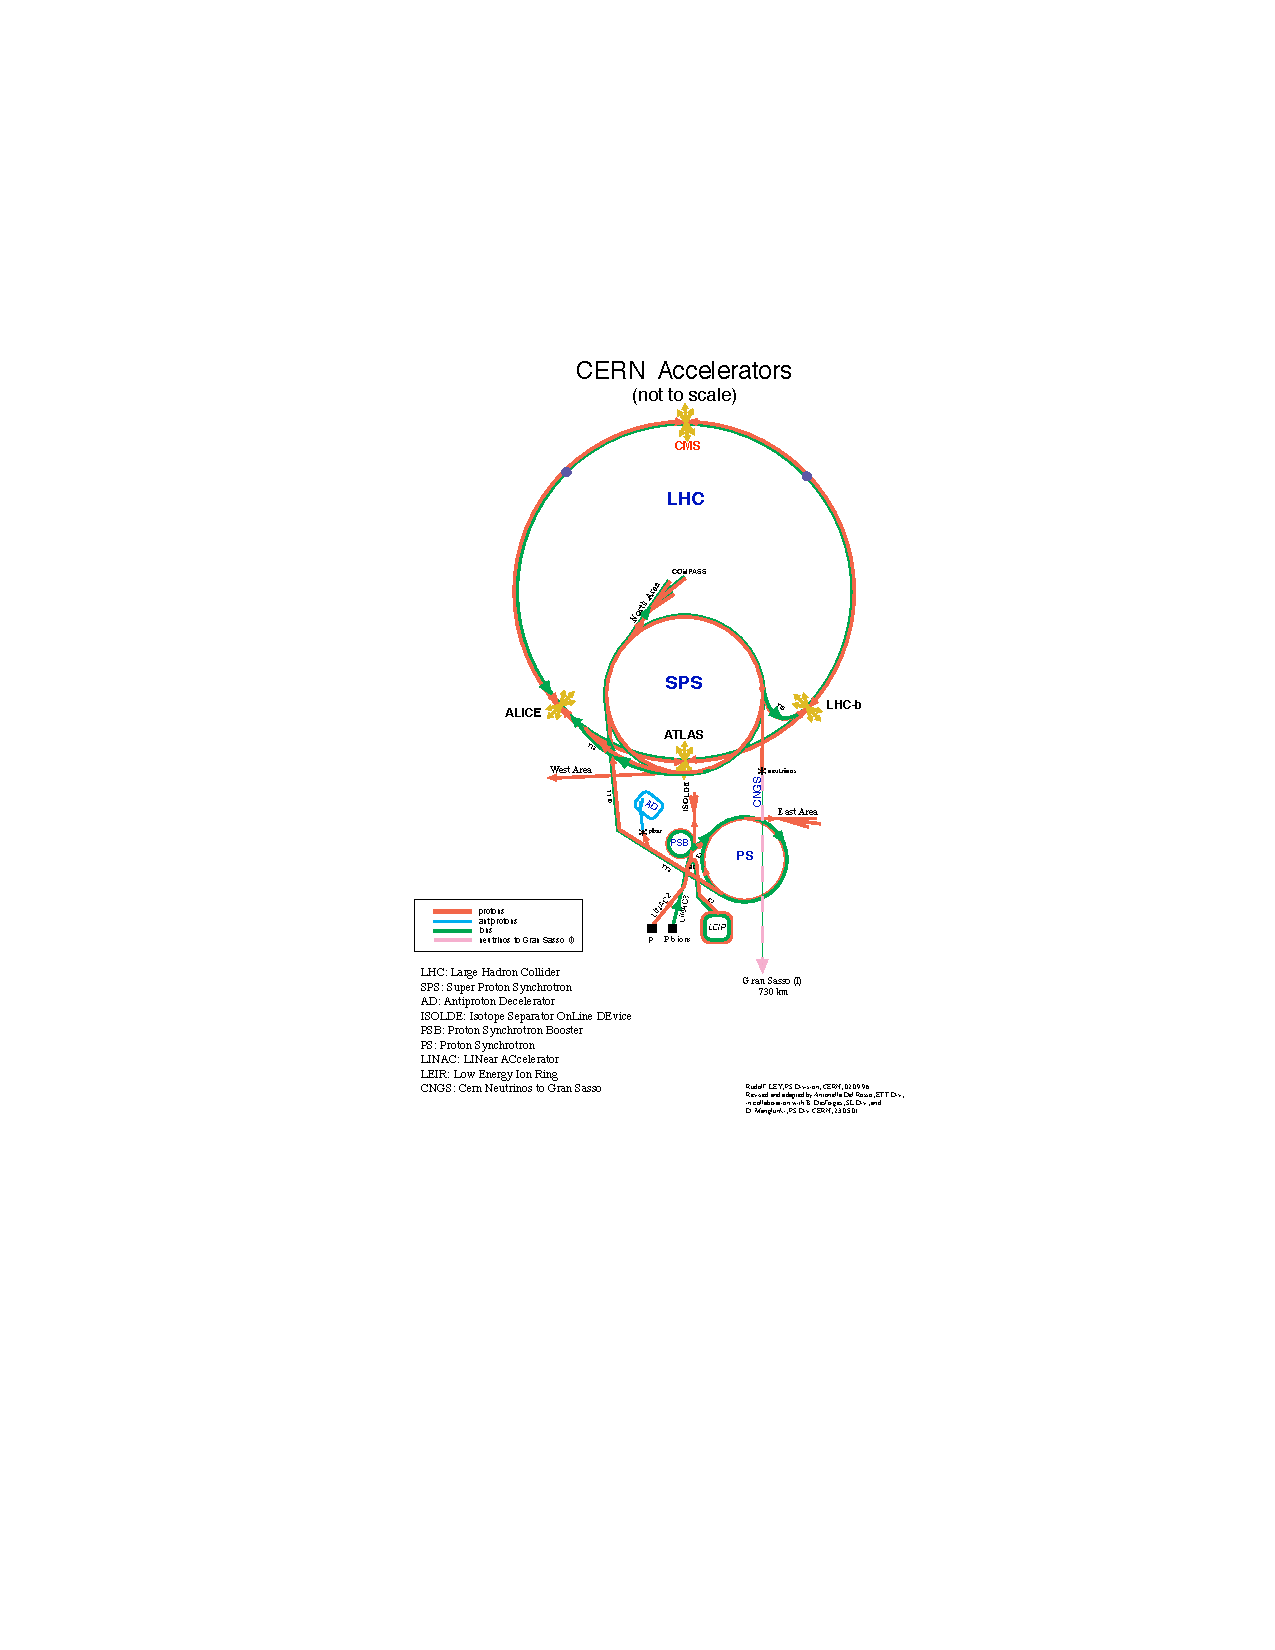
\includegraphics{figures/Detector/lhc_accel.pdf}
  \caption{An overview schematic of the LHC accelerator subsystems.} 
  \label{fig:lhc_accel}
\end{figure}
\FloatBarrier


As many new physics models predict cross-sections below the weak scale it was important to design the LHC to be capable of collecting enough data, by running in high luminosity conditions. The machine luminosity depends only on beam parameters:

\begin{equation}
L=\frac{N_{p}^{2}f}{4\epsilon\beta^{*}}F
\end{equation}

where $N_{p}$ is the number of protons per bunch, f is the bunch crossing frequency, $\epsilon$ is the transverse beam emittance, $\beta^{*}$ is the amplitude function at the collision point, and F is the geometric luminosity reduction factor due to the beams crossing at an angle (rather than head-on). 

\chapter{The ATLAS Detector}
The ATLAS detector measures the position, momentum and energy of particles produced in the proton collisions by using magnetic fields, silicon detectors, sampling calorimeters, and gaseous wire detectors. It is located approximately 100 m underground at Point-1 around the LHC beam line and weighs 7000 metric tons. The detector is 46 m long, 25 m high, 25 m wide  as shown in Figure \ref{fig:atlas_detectors}. The detector can be divided into three subsystems: the Inner Detector (ID), the Calorimeters, and the Muon Spectrometer (MS). Figure \ref{fig:particle_detection} shows an overview of how different particles interact in the detector.
\begin{figure}[h!]
  \centering
  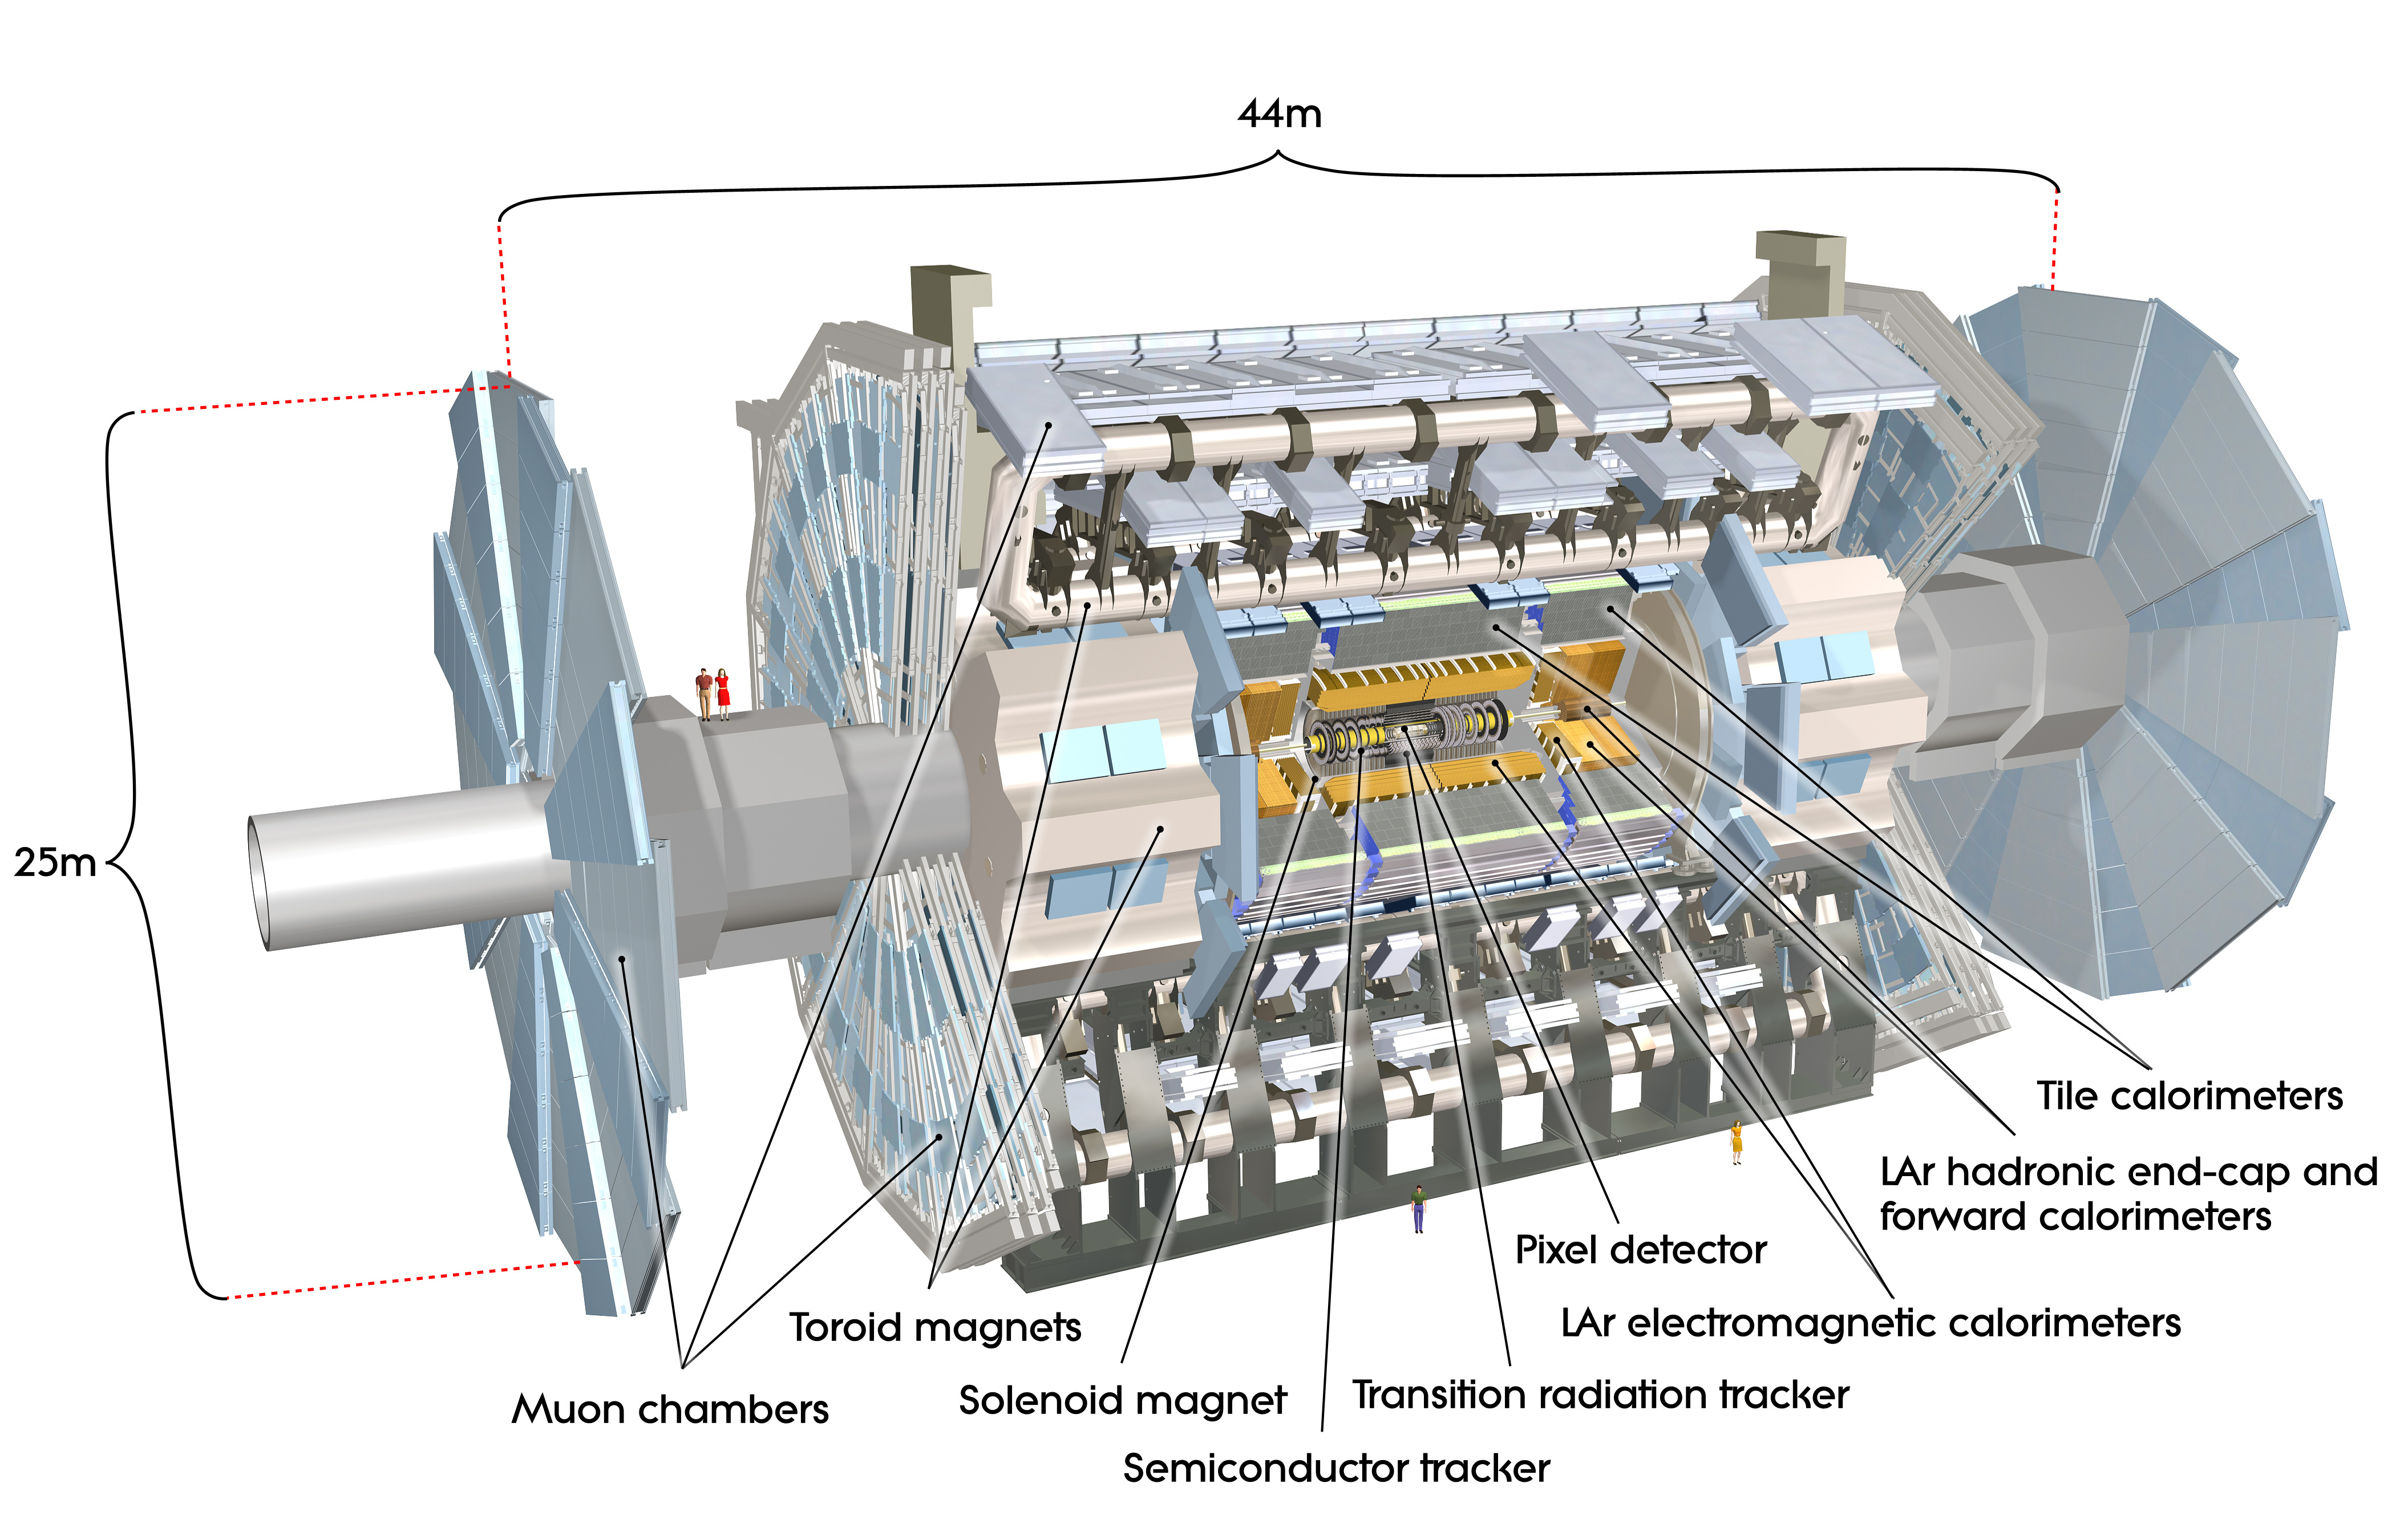
\includegraphics[width=\hsize]{figures/Detector/atlas.jpg}
  \caption{Overview schematic of the ATLAS detector.} 
  \label{fig:atlas_detectors}
\end{figure}
\FloatBarrier


\begin{figure}[h!]
  \centering
  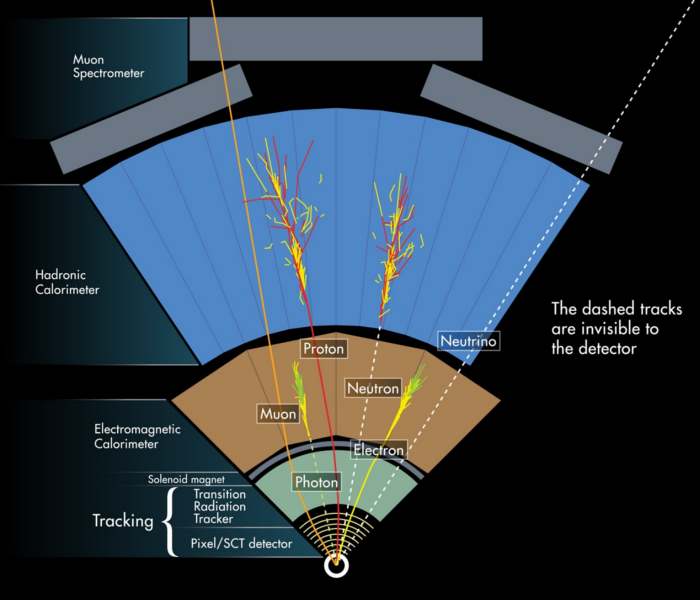
\includegraphics[width=\hsize]{figures/Detector/particle_detection_atlas.png}
  \caption{A simplified schematic of how different particles interact and are detected within ATLAS.} 
  \label{fig:particle_detection}
\end{figure}
\FloatBarrier

\section{Coordinate System}
The trajectory of particles within ATLAS is measured relative to the nominal interaction point. The $z$-axis points along the beam line, such that when the LHC is viewed from above, the counter-clockwise circulating beam points along the positive-$z$ direction. The $x-y$ plane is transverse to the beam line, with the positive x-axis pointing towards the center of the LHC ring. The positive $y$-axis points vertically upward. The azimuthal angle, $\phi$, is the angular distance about the $z$-axis, with $\phi=0$ along the $x$-axis. The polar angle from the $z$-axis is denoted as $\theta$.  However, this quantity is not Lorentz invariant, like rapidity, $y=\frac{1}{2}\ln\frac{E+p_{z}}{E-p_{z}}$, where $E$ is the energy of the particle considered, and $p_{z}$, is it's momentum along the $z$-axis. Pseudorapidity is preferred as $\Delta \eta$ is invariant under boosts along $z$ and particle production is approximately invariant under $\eta$. For massless particles, rapidity and a related quantity, pseudorapidity, are the identical. The pseudorapidity is defined as: $\eta = -\ln \tan(\frac{\theta}{2})$.  This quantity is preferred as it is purely a geometric quantity, independent of particle energy. Angular separation between particles in ATLAS are given by $\Delta R = \sqrt{\Delta \eta^{2}+\Delta \phi^{2}}$. The distance from the beamline is given by $r=\sqrt{x^{2}+y^{2}}$
 
\section{Inner Detector}
The Inner Detector (ID) was designed to identify and reconstruct vertices, distinguish pions from electrons, and measure the momentum of charged particles. The ID uses three different technologies for particle reconstruction: the Pixel Detector, Semiconductor Tracker (SCT), and the Transition Radiation Tracker (TRT), shown in Figure \ref{fig:ID} and \ref{fig:barrelID}. The entire ID is immersed in a 2T solenoidal magnetic field parallel to the $+z$-axis, causing charged particles to bend in the transverse-plane, allowing particle momentum measurements. 

\begin{figure}[h!]
  \centering
  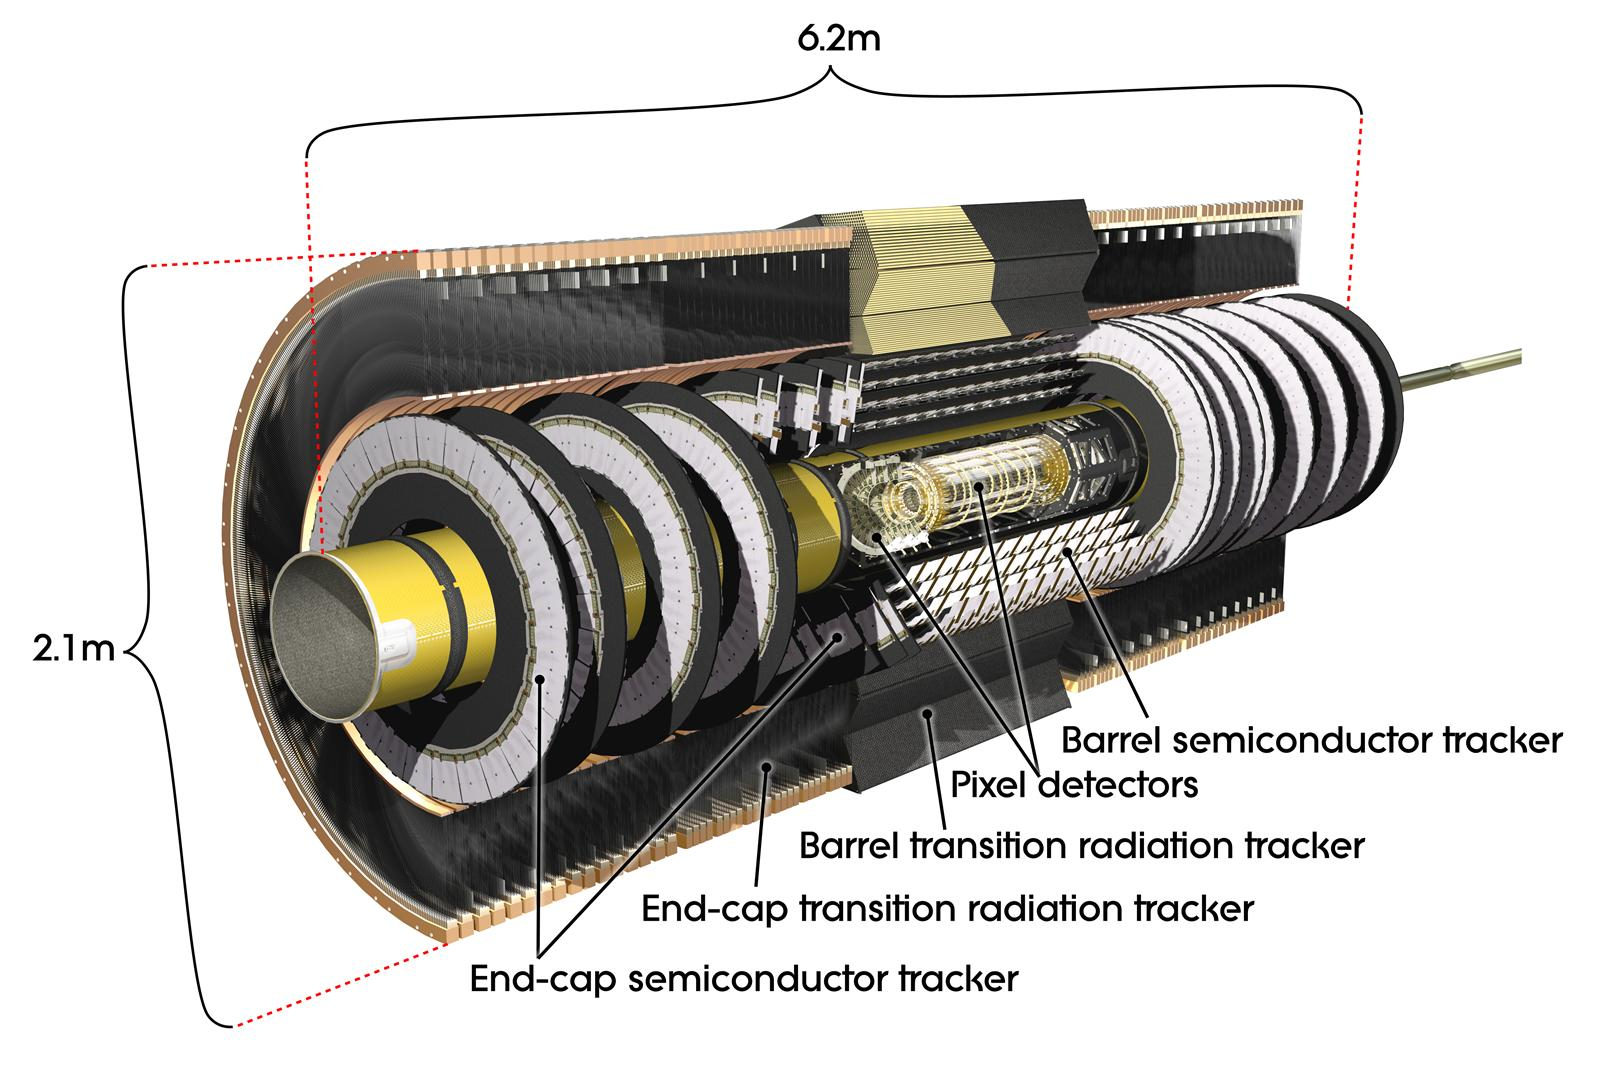
\includegraphics[width=\hsize]{figures/Detector/tracker_layout.jpg}
  \caption{Layout of ATLAS Inner Detector} 
  \label{fig:ID}
\end{figure}
\FloatBarrier


\begin{figure}[h!]
  \centering
  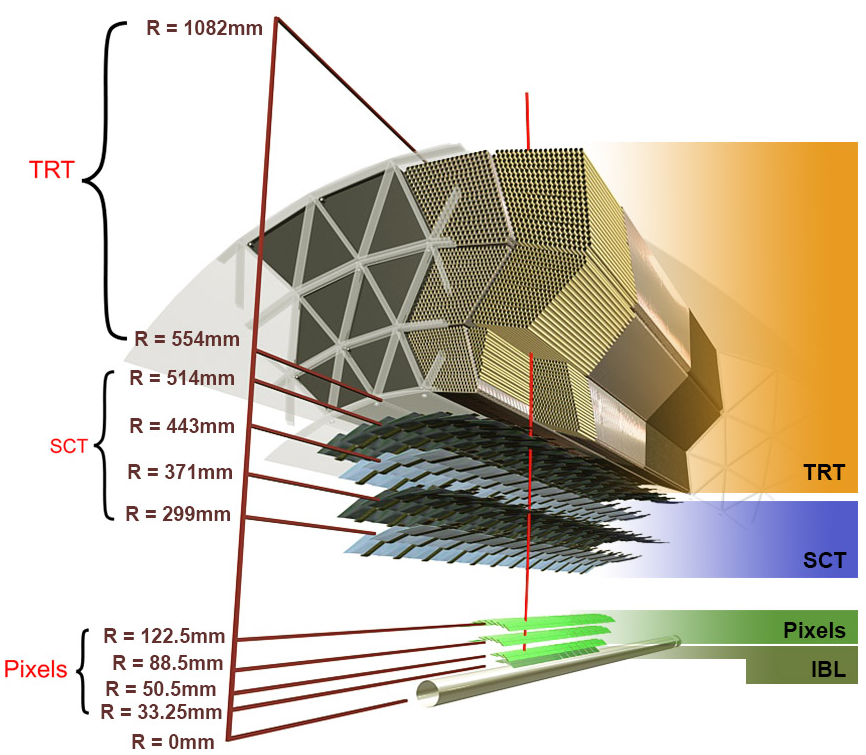
\includegraphics[width=\hsize]{figures/Detector/tracker_barrel.png}
  \caption{Layout of ATLAS ID Barrel System.} 
  \label{fig:barrelID}
\end{figure}
\FloatBarrier


\subsection{Pixel Detector}
The pixel detector consists of four barrel layers between r = 32.7 and 122.5 mm, extending to $|z|=400.5 $mm. The remaining detectors are arranged in barrels and forward and backward rings. The innermost pixel barrel, the Insertable b-Layer (IBL), only extends to $|z|=332$ mm. The pixel detectors closer to the beam line (larger $\eta$ values) consists of six parallel cylindrical rings of pixel detectors transverse to the beam line. The entire pixel detector consists of 1744 identical pixel sensors each with 46080 readout channels, totaling about 80 million individual pixels. Most of the pixel sensors are $50\times400\mu m^{2}$.  Each pixel has a position resolution of 14$\mu$m in $\phi$ and 115 $\mu$m in the $z$ direction.
\subsection{Semiconductor Tracker}
The SCT is located outside the pixel detector and has the same barrel and endcap geometry as the pixel detector. SCT sensors are 80$\mu$m $\times$ 12 cm with a 80$\mu$m strip pitch. In the barrel the strips are parallel to the $z$-axis and are segmented in $\phi$. In the endcaps, the strips extend radially. Sensors are grouped in modules containing two layers of strips rotated 40 mrad with respect to each other. This offset allows for the two-dimensional position of a track to be determined by identifying the crossing point of the strips that registered a hit. SCT modules measure tracks with an accuracy of 17 $\mu$m in $r-\phi$ and 580$\mu$m in $z(r)$ in the barrel (end-cap) region.
\subsection{Transition Radiation Tracker}
The transition radiation tracker (TRT), enveloping the SCT, is a gaseous straw-tube tracker mainly used for electron/pion track separation. Each straw is 4 mm in diameter and filled with a Xe-C$O_{2}$-$O_{2}$ gas mixture. An anode wire at the center of the straw is held at ground potential, while the walls of the straw are kept at -1.4kV. When a charged particle passing through the TRT ionizes the gaseous mixture, the resulting ions form an avalanche on the anode wire with a gain of $\sim 10^{4}$. The signal from the anode wire is then digitized and discriminated. Signals passing a low threshold cutoff are used to distinguish noise from tracks. Signals passing a high threshold cutoff are sensitive to transition radiation (TR). TR photons are emitted when charged particles pass between materials with different dielectric constants. The probability that a charged particle with energy $E$ and mass $m$ passing between two materials emits a TR photon in the keV range is proportional to $\gamma=E/m$. In the TRT staws these often then convert via the photoelectric effect, causing a large avalanche triggering the high-threshold. Since electrons have a smaller mass than pions, electron tracks are more likely to trigger the high threshold. This then provides discrimination between electrons and charged hadrons.

The barrel region of the TRT extends from $r=$563-1066 mm and $|z| < 712$ mm. Barrel Straws are 144 cm long (divided  $\sim \eta \approx 0$) and orientated parallel to the beam direction. End-cap straws extend radially and are 37 cm long. There are 53,544 straws in the barrel and 160,000 straws in the end-caps. Radiator mats of polypropylene/polyethylene fibers in the barrel are aligned perpendicular to the barrel straws (with holes for the straws to pass through). In the end-cap region, radiator foils are layered between the radial TRT straws. 

The arrival time of the signal pulse is sensitive to the distance between the charged particle track and the anode wire and allows for a hit resolution of 130$\mu$m. The TRT extends to $|\eta| = 2.0$ and provides about 36 hits per track.
\section{Calorimeters}
The ATLAS electromagnetic and hadronic calorimeters (EMC and HCAL, respectively) absorb and measure the energy of high energy hadrons, photons, and electrons with $|\eta| < 4.9$. Both systems use sampling calorimeters which consist of alternating layers of dense absorbing and active layers. In the absorbing layer particles interact and lose energy, creating showers. These showers are then detected and measured in the active layer. The amount of charge measured in the active material scales with the energy of the incident particle, and thus provides a measurement of the particle's energy. An overview of the layout of the calorimeter system is shown in Figure \ref{fig:calo_overview}.

The EMC measures and contains the energy of electromagnetically interacting particles. It consists of layered accordion-shaped Lead absorber plates and electrodes immersed in liquid Argon with 170k channels.. Using accordion-shaped electrode and absorbers ensures $\phi$ symmetry and coverage. The EMC is composed of a barrel part ($|\eta| < 1.475$), two end-caps ($1.375<|\eta| < 3.2$), and a presampler ($|\eta| < 1.8$).  The presampler, containing only liquid Argon, corrects for upstream energy losses of electrons and photons. The EMC barrel is segmented into three layers. The first layer has finest segmentation with readout cells extending $\Delta \eta \times \Delta \phi = 0.025/8 \times 0.1$. This provides a precise shower measurements used to separate prompt photons from $\pi^{0} \rightarrow \gamma \gamma$ decays. The second layer has coarser segmentation and is approximately 16 radiation lengths long. A radiation length is the average distance an electron travels before losing all but 1/$e$ of its energy to bremsstrahlung. The last layer is the most coarse and measures the tail of the electromagnetic shower. A schematic of the ECAL is shown in Figure \ref{fig:ecal}. 

The hadronic calorimeter located outside the EMC and is used to contain and measure the energy of hadronically interacting particles. It consists of a tile calorimeter (TileCal), hadronic end-cap calorimeter (HEC), and liquid Argon forward calorimeter (FCAL). TileCal is located behind the LAr EMC and uses steel absorbers and liquid Argon as the active material. TileCal consists of three barrel layers in the central and forward regions, extending up to $|\eta| < 1.7$. Photons generated from hadronic interactions are collected via wavelength-shifting fibers connected to photomultiplier tubes, as shown in Figure ~\ref{fig:hcal}. The HEC lies behind the EMC endcap wheels. It uses copper absorbers and liquid Argon as the active material and covers $1.5 < |\eta| < 3.2$. Finally, the FCAL covers $3.1 < |\eta| < 4.9$ and consists of three modules all using liquid Argon as the active material. The first module uses copper absorber and was designed for electromagnetic measurements. The second and third modules consist of tungsten absorber and are used to measure the kinematics of hadronically interacting particles. A schematic of the HCAL is shown in Figure \ref{fig:hcal}. 

\begin{figure}[h!]
  \centering
  \includegraphics[width=\hsize]{figures/Detector/calo_overview.pdf}
  \caption{Overview of ATLAS electromagnetic and hadronic calorimeters.} 
  \label{fig:calo_overview}
\end{figure}
\FloatBarrier


\begin{figure}[h!]
  \centering
  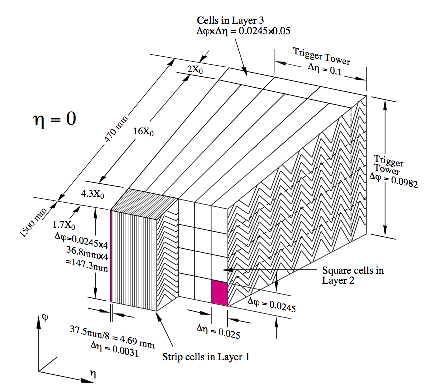
\includegraphics[width=\hsize]{figures/Detector/ecal.pdf}
  \caption{Schematic of ECAL.} 
  \label{fig:ecal}
\end{figure}
\FloatBarrier




\begin{figure}[h!]
  \centering
  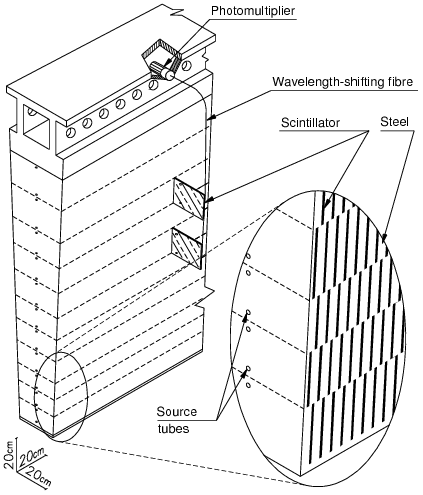
\includegraphics[width=\hsize]{figures/Detector/hcal.png}
  \caption{Schematic of HCAL.} 
  \label{fig:hcal}
\end{figure}
\FloatBarrier


The energy resolution of the calorimeter subsystems are:

$\frac{\sigma_{E}}{E}=\frac{10\%}{\sqrt{E}}\bigoplus \frac{0.3\%}{E}\bigoplus 0.4\%$ Electromagnetic Calorimeter

$\frac{\sigma_{E}}{E}=\frac{50\%}{\sqrt{E}}\bigoplus \frac{1.8\%}{E}\bigoplus 3\%$ Hadronic Calorimeter


\section{Muon Spectrometer}
The muon spectrometer (MS) is the outermost detector system in ATLAS. Muons with a $p_{T}>4$ GeV are energetic enough to reach the MS. To measure the momentum of these muons barrel and end-cap toroid magnets are used covering $|\eta| < 1.4$ and $1.6<|\eta|<2.7$. For $1.4 < |\eta| < 1.6$, a combination of the barrel and end-cap toroidal magnetic fields bend muon trajectories. The detector in the barrel region form three concentric rings at $R=5, 7.5, 10$ m and are segmented in $\phi$ to accommodate the magnets. The end-cap region consists of three circular planes perpendicular to $z$ and located at $|z|=7.4, 14, 21.5$ m from the interaction region. An additional detector at $|z|=10.8$ m covers the transition region between the barrel and end-cap.

The MS readout consists of four subsystems: Monitored Drift Tubes (MDT), Cathode Strip Chambers (CSC), Resistive Plate Chambers (RPC), and Thin Gap Chambers (TGC). The first two subsystems are used primarily for measuring muon track parameters, while the RPC and TGC subsystems are used for muon triggering. A schematic of this system is shown in Figure ~\ref{fig:muonsys}. 

The MDT subsystem consists of precision tracking chambers for $|\eta|<2.7$, except for the inner most end-cap layer ($2.0 < |\eta| < 2.7$), where CSCs are used. The basic unit of MDT chambers are thin walled Aluminum tubes with a diameter of 3 cm and length of 0.9-6.2 m. These tubes are filled with a mixture of Ar-CO$_{2}$ gas with a  50$\mu$m W-Rn wire running down the center of the tube, which is kept at 3080 V. Since the maximum drift time of these chambers is $\sim$ 700 ns, they are not used for triggering. MDT chambers consist of 3-4 layers of tubes mounted on a rectangular support system, as seen in Figure ~\ref{fig:muon_mdt}, orientated along $\phi$ to measure the coordinate in the bending plane of the magnetic field with a resolution of 35 $\mu$m.

The MDT subsystem can only handle hit rates below 150 Hz/cm$^{2}$. For this reason, CSCs are used in the innermost end-cap layer where hit rates are larger. CSCs can handle hit rates up to 1000Hz/cm$^{2}$. CSC are multiwire proportional chambers. These chambers are filled with a Ar-C$O_{2}$ gas mixture and evenly spaced wires kept at 1900 V. These wires are orientated in the radial direction but not read out. Instead on one side of the cathode are copper strips parallel to the wires, measuring $\eta$, while on the other side of the cathode are strips parallel to the wires measuring $\phi$. The width between strips is approximately 1.5 mm providing a resolution of 60 $\mu$m in the bending-plane and 5 mm in the non-bending plane. 

Since the CSC and MDT systems do not have prompt timing signals, the RPC and TGC systems are used for triggering. The RPC system is used in the barrel region ($|\eta| < 1.05$). RPC consist of two parallel resistive plates separated by a 2 mm insulated spacer with 100 mm spacing kept at 9.8 kV, as shown in Figure \ref{fig:muon_rpc}. A gaseous mixture of C$_{2}$H$_{2}$F$_{4}$, C$_{4}$H$_{10}$, and SF$_{6}$ fills the space between the two plates. Metallic strips on the outer faces of the plates are used to read out signals produced by the gas ionizing. The middle barrel layer consists of two layers of RPCs on either side of the MDT layer and one layer on the outermost MDT layer. Each layer contains two orthogonal sets of metallic strips providing $\eta$ and $\phi$ measurements. The timing resolution of RPCs is 1.5 ns, and therefore may be used to identify bunch crossings. 

Finally, the TGCs are used in the end-cap regions and are primarily used to provide L1 trigger decisions and $\phi$ measurements. TGCs are multi-wire proportional chambers consisting of arrays of gold-coated tungsten wires placed between two cathode planes. These wires are separated by 1.8 mm and cathodes are 1.4 mm from the wires. Orthogonal to the wires, on the opposite side of the cathode plane are copper strips held at 2900 V. The chambers are filled with a mixture of CO$_{2}$ and n-pentane gas, the latter acts as a quenching gas to prevent avalanches initiated by secondary $\gamma$-rays from the primary avalanche. Figure ~\ref{fig:muon_tgc} is a schematic of a TGC. The timing resolution of TGCs is less than 25 ns and therefore they are used for bunch crossing measurements. 

\begin{figure}[h!]
  \centering
  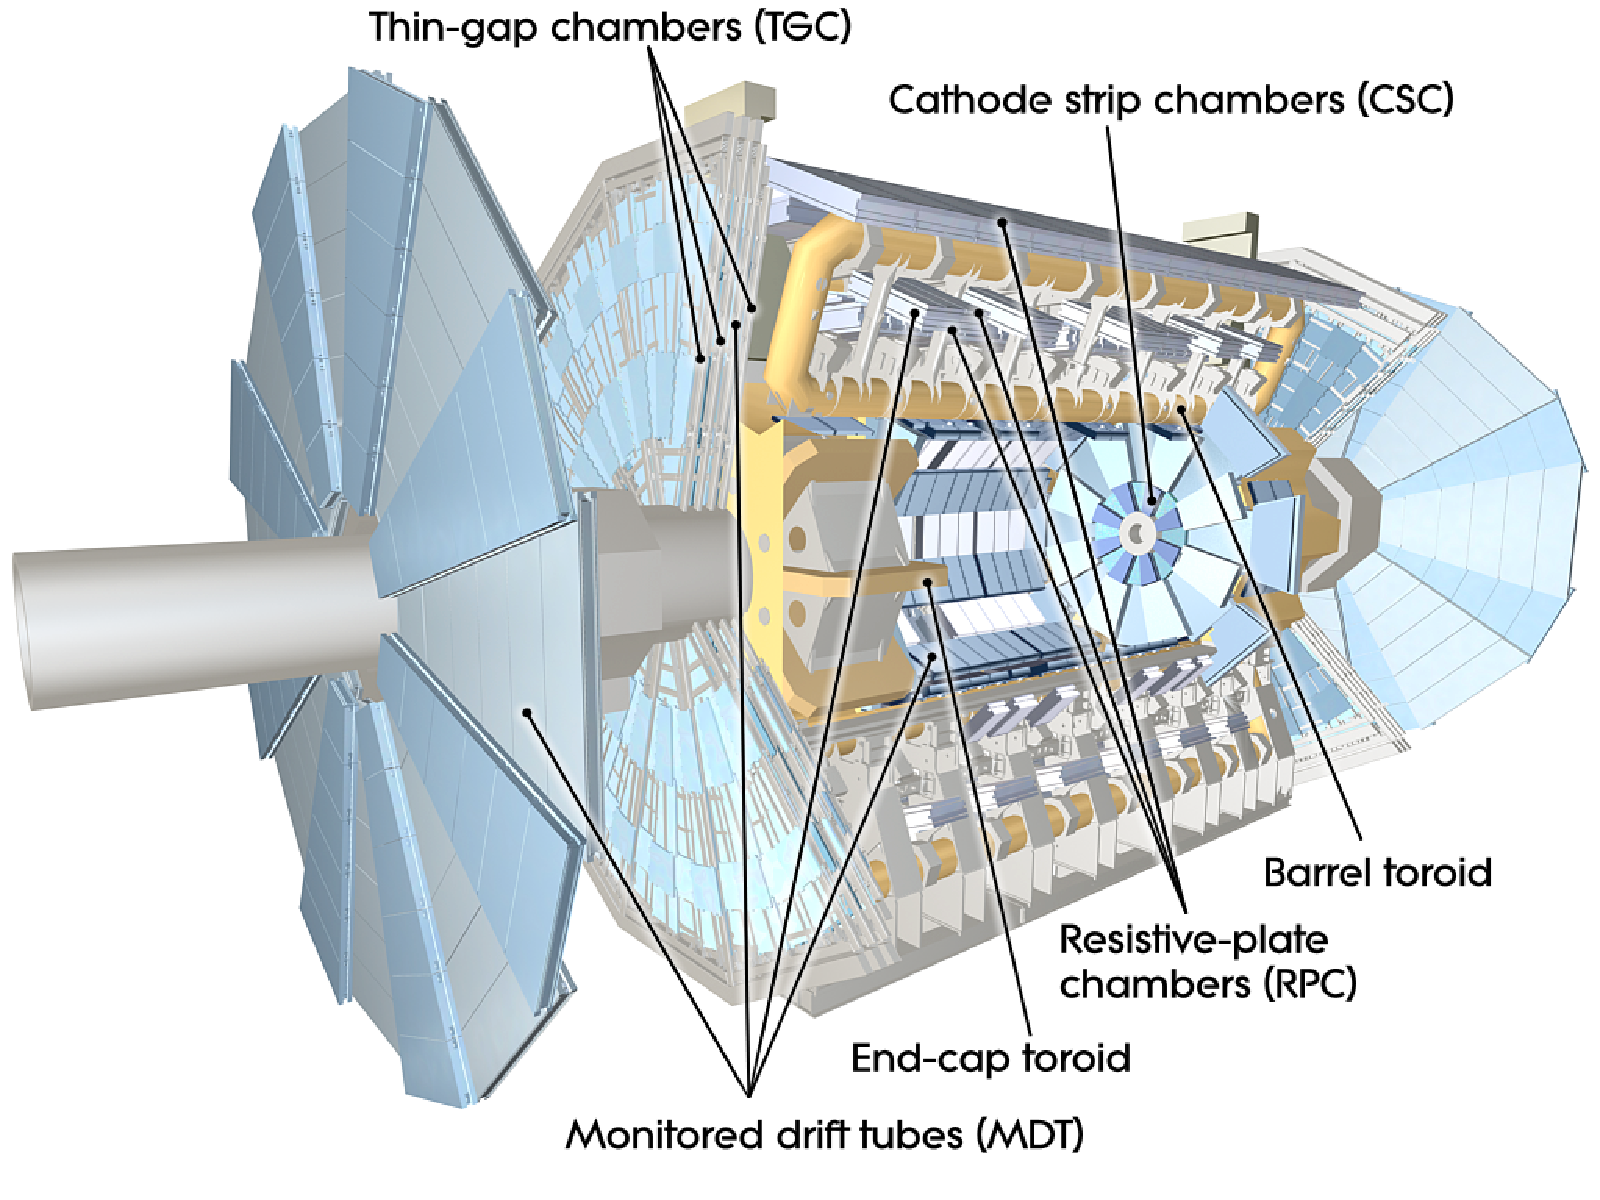
\includegraphics[width=\hsize]{figures/Detector/muonsys.pdf}
  \caption{Schematic of Muon Spectrometer [cite G35]} 
  \label{fig:muonsys}
\end{figure}
\FloatBarrier


\begin{figure}[h!]
  \centering
  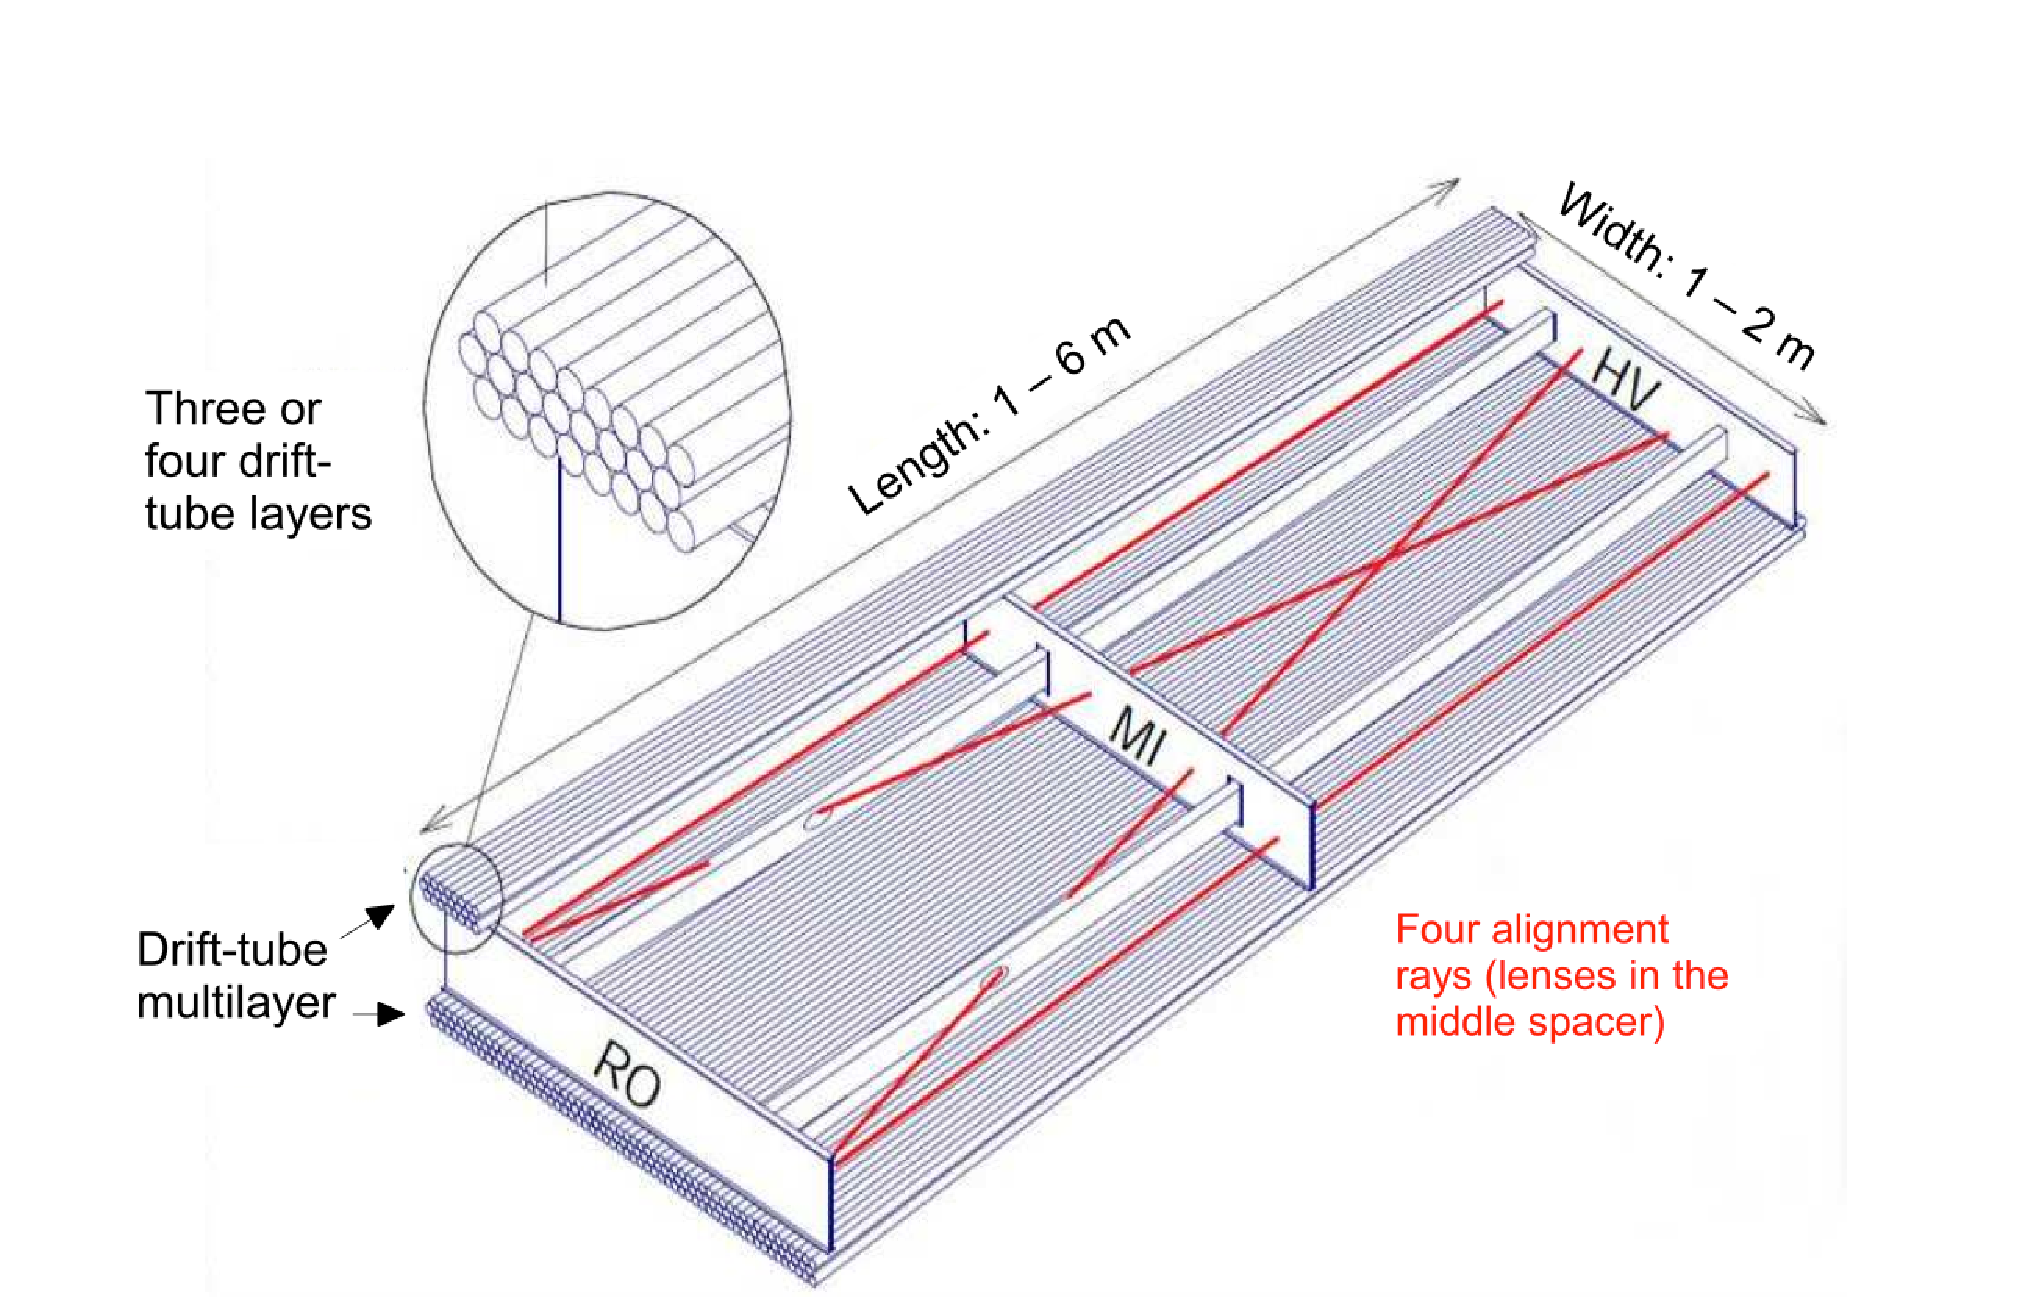
\includegraphics[width=\hsize]{figures/Detector/muon_mdt.pdf}
  \caption{Schematic of MDT chamber. [cite G35]} 
  \label{fig:muon_mdt}
\end{figure}
\FloatBarrier


\begin{figure}[h!]
  \centering
  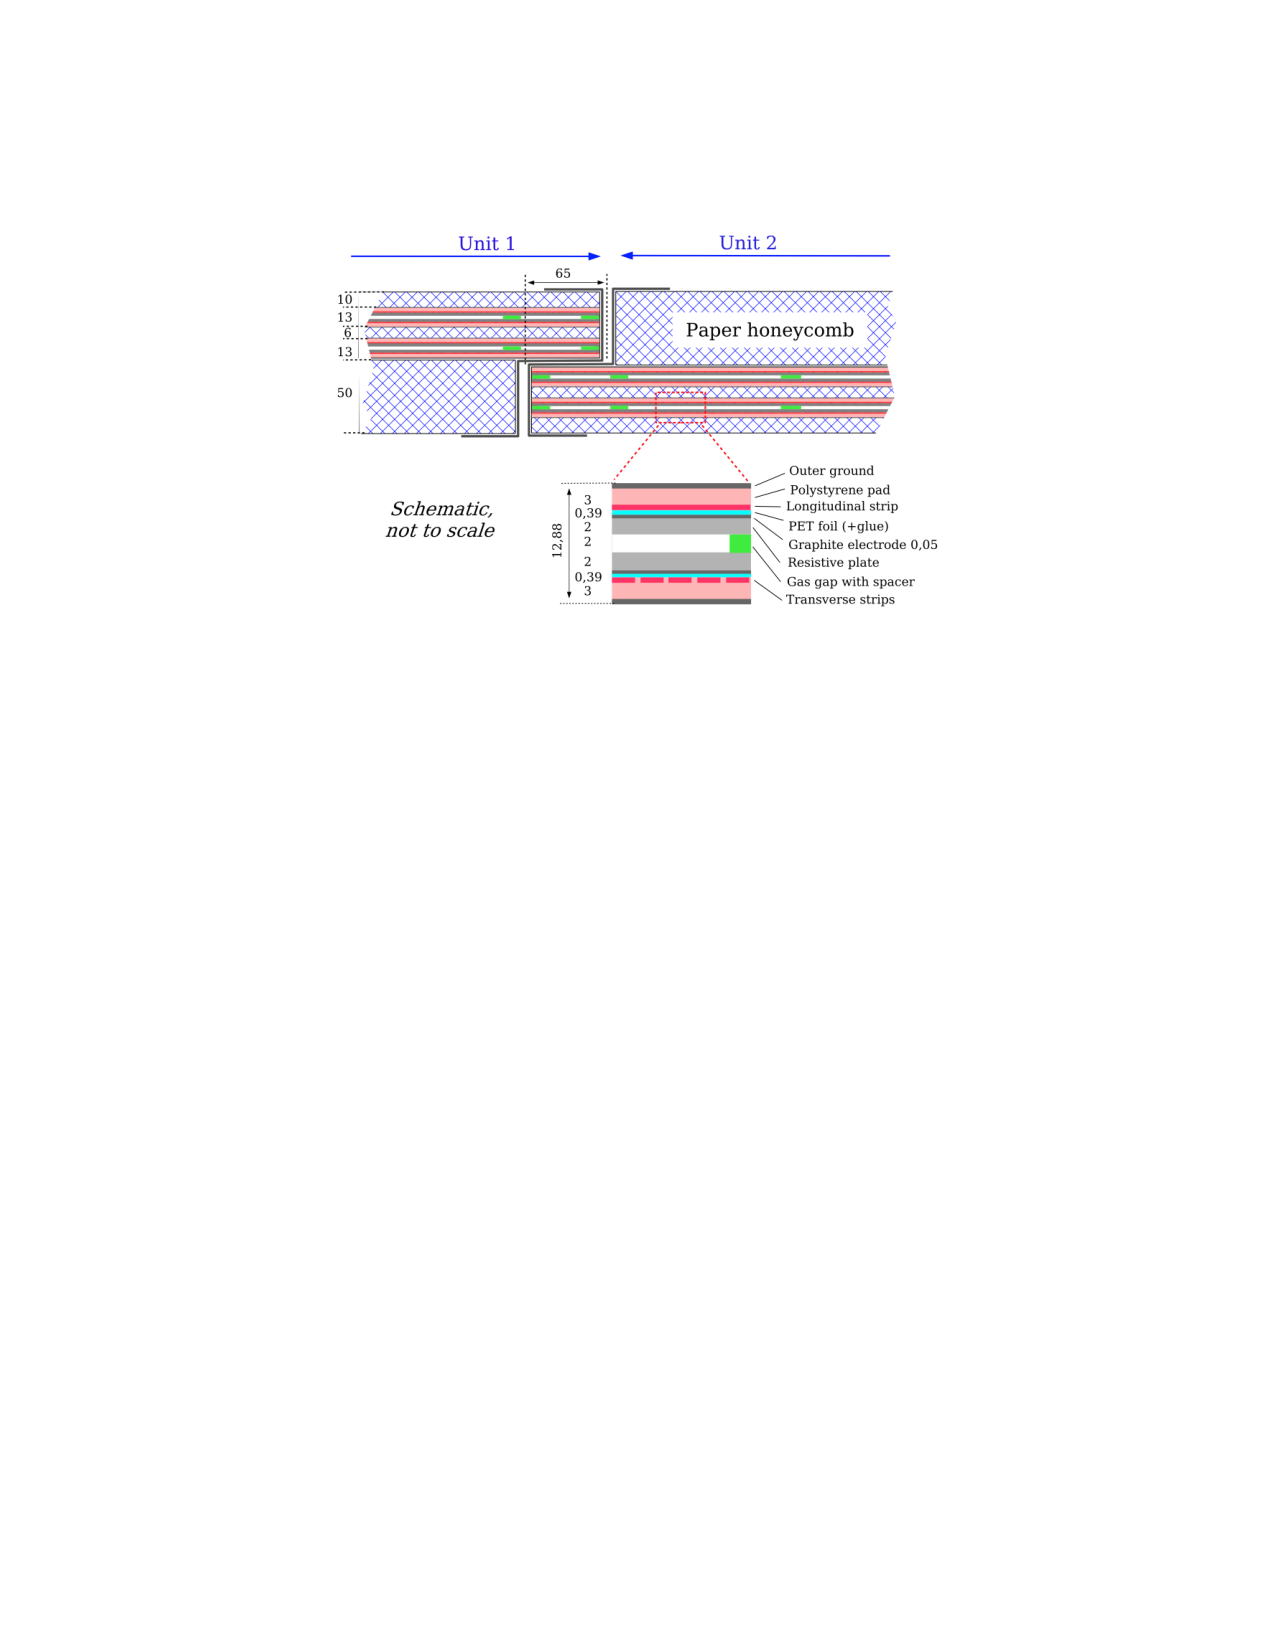
\includegraphics[width=\hsize]{figures/Detector/muon_rpc.pdf}
  \caption{Schematic of RPC chamber, which is used for triggering in the central region of the detector [cite G35].} 
  \label{fig:muon_rpc}
\end{figure}
\FloatBarrier



\begin{figure}[h!]
  \centering
  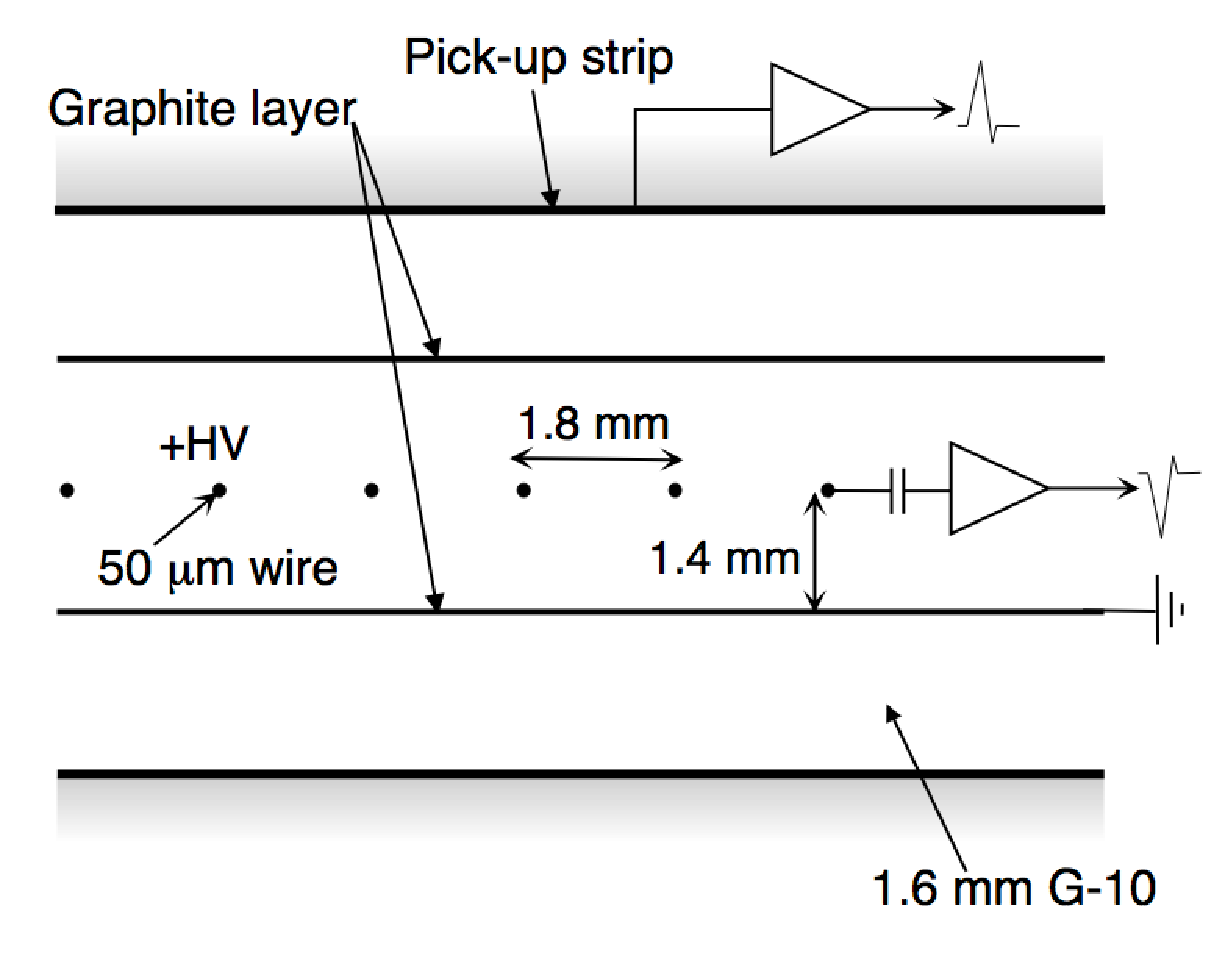
\includegraphics[width=\hsize]{figures/Detector/muon_tgc.pdf}
  \caption{Schematic of TGC chamber, which is used for triggering in the muon end-cap region. [cite G35]} 
  \label{fig:muon_tgc}
\end{figure}
\FloatBarrier

\section{Magnet System}
A particles with charge, q, and velocity v, moving in magnetic field, B, experiences a force, $F= qv\times B$. This force can cause charged particles to have a curved trajectory in magnetic fields, which the ID and MS use to determine the particles $p_{T}$. The central solenoid provides the magnetic field for the ID and the toroidal magnets provide the magnetic field for the MS.

The layout of the magnet system is shown in Figure \ref{fig:atlas_magnets}. The central solenoid consists of a single-layer Al-stabilized NbTi conductor coil wound inside an Al support cylinder. The solenoid is 5.8 m long, 50 cm thick and has an inner radius of 1.23 m. It is cooled to 4.5 K to reach superconducting temperatures and shares the liquid argon calorimeter vacuum vessel to minimize material in the detector. A current of 7.730 kA produces a 1.998 T solenoidal magnetic field, pointing in the +$z$ direction. 

The toroidal magnet system consists of a barrel and two end-cap toroidal magnets used to create a magnetic field outside the calorimeters that is orientated along $\phi$. Each barrel toroid is 25.3 m long with an inner and outer diameter of 9.4 and 20.1 m and weighs 830 tonnes. Endcap toroids are 5 m long with an inner and outer radius of 1.65 and 10.7 m. Both toroid systems use Al-stabilized Nb/Ti/Cu conductors. The magnetic field strength in the barrel and endcap regions are 0.5 and 1 T, respectively.

\begin{figure}[h!]
  \centering
  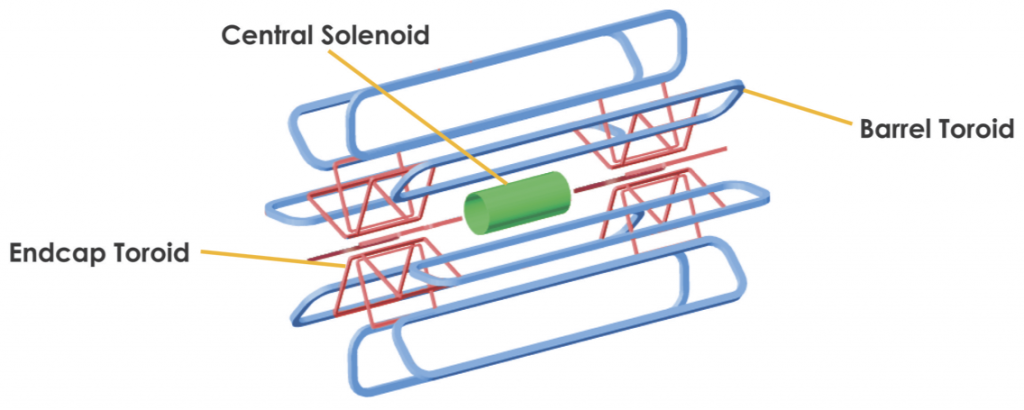
\includegraphics[width=\hsize]{figures/Detector/atlas_magnets.png}
  \caption{Layout of ATLAS magnet systems.} 
  \label{fig:atlas_magnets}
\end{figure}
\FloatBarrier


\section{Trigger System}
Since collisions occur every 25 ns and reading out all detector channels and storing that information is not currently feasible (would require saving 60 million megabytes per second), the majority of events are not kept for analysis. ATLAS uses a multi-stage trigger system to select approximately 1,000 of the 1.7 billion collisions that occur each second (corresponding to a rate of 1 kHz from the 40 MHz proton collision rate). The first stage of the trigger system is the hardware level (L1) trigger. This trigger reduces the event rate to $\sim$100 kHz by identifying Regions-of-Interest (ROIs) containing high $p_{T}$ leptons, photons, jets, or $E_{T}^{miss}$ by using information from RPCs, TGCs, and calorimeters to make a 2.5 $\mu$s decision. This information is then passed to a high-level trigger (HLT) which further decreases event rates to $\sim$ 1 kHz. The HLT uses finer granularity measurements from the MS and ID to preform simplified offline reconstruction to decide which events to keep.

%\chapter{LHC and ATLAS Detector}
%\label{ch:detector}
\chapter{LHC}
The Large Hadron Collider (LHC) is the highest-energy particle collider in the world. It was designed to expand the frontier of high energy particle collisions in energy and luminosity. This enables LHC experiments to test the Standard Model and search for new physics at higher energies than tested with previous colliders. Collisions at higher energies not only produce more massive particles but also more weakly interacting particles. Fig ~\ref{fig:xs_scaling} shows production cross sections for various processes at hadron colliders. The rate for electroweak physics processes including $W$ and $Z$ scale with the center-of-momentum energy, $\sqrt{s}$.

The LHC consists of a 26.7 km (17 miles) ring, approximately 100 m underground, outside Geneva, Switzerland. Counter-circulating proton (and occasionally heavy ions) beams collide inside four experiments along the beam line: ATLAS, CMS, LHCb, ALICE. ATLAS and CMS are general purpose detectors designed to explore the high energy frontier. LHCb is designed to study the physics of $b$-quarks. ALICE specializes in studying heavy ion collisions. 


\begin{figure}[h!]
  \centering
  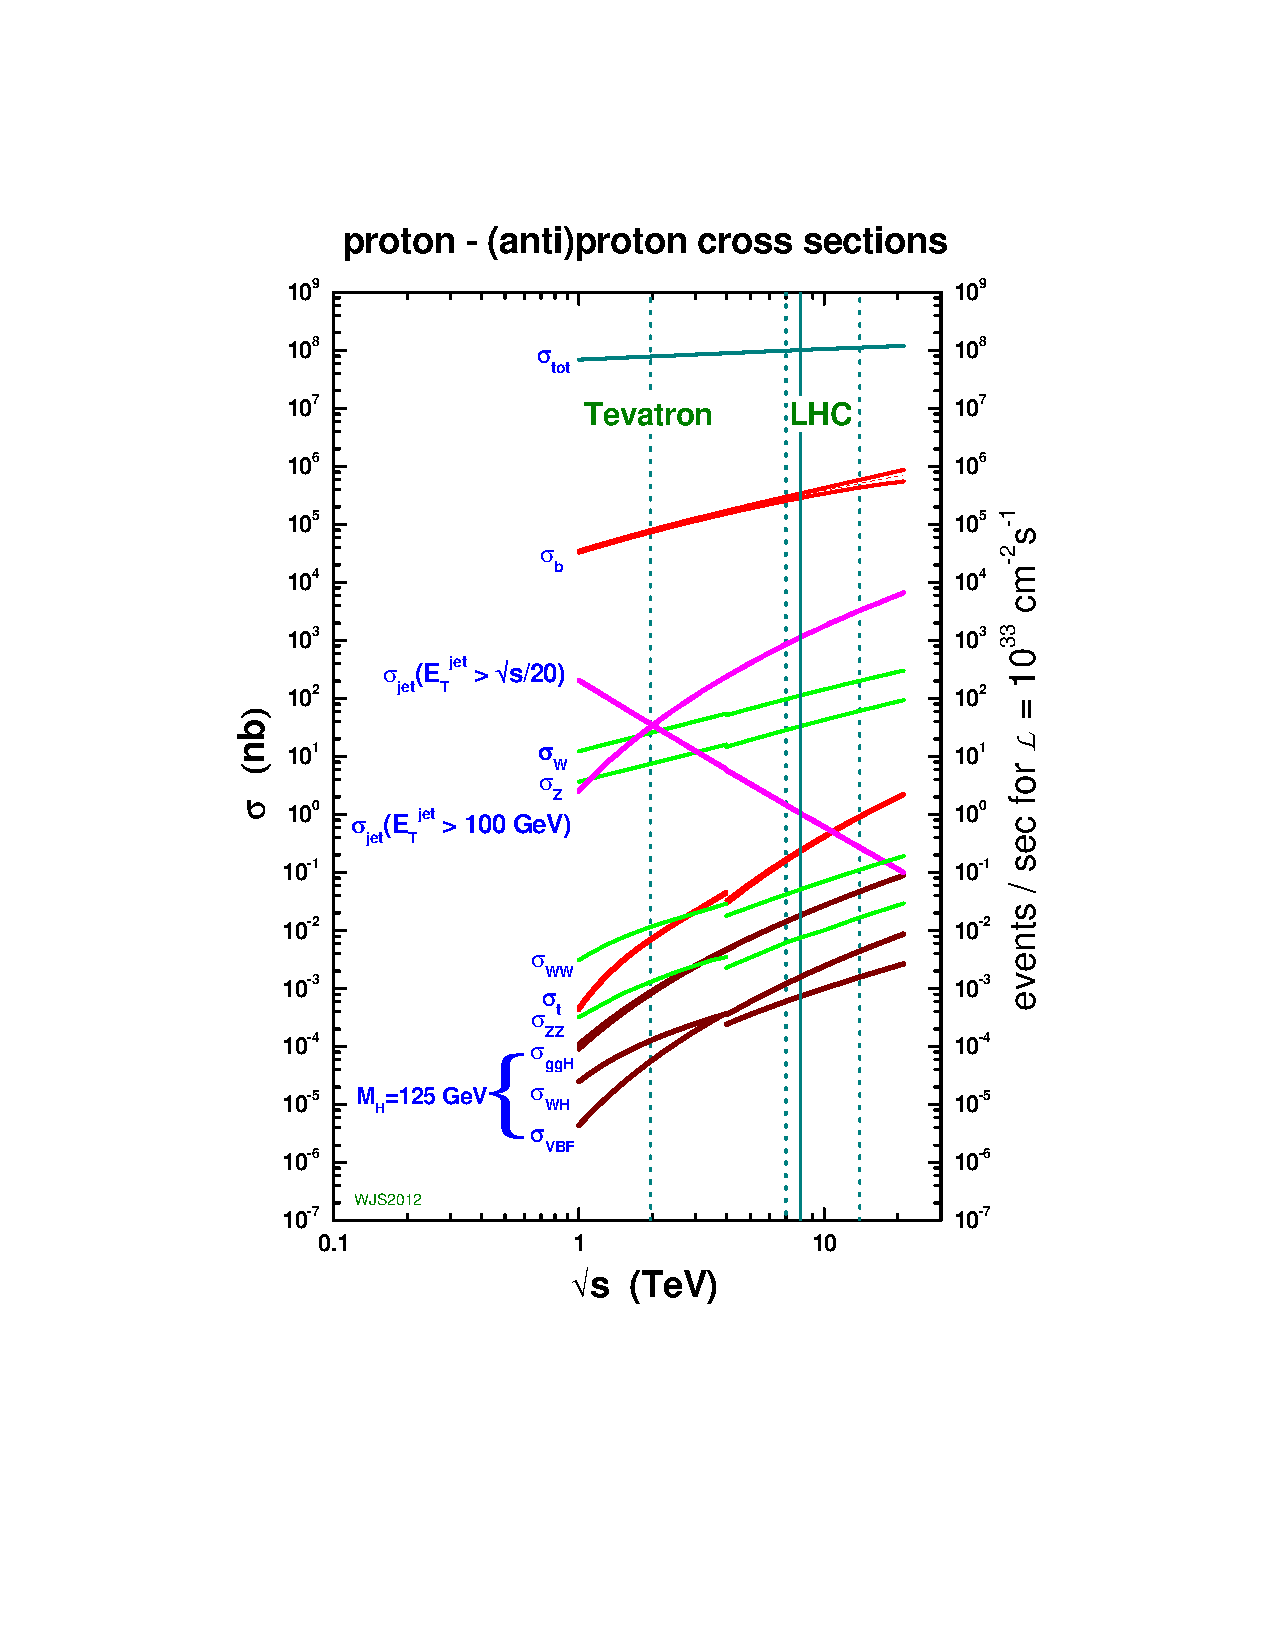
\includegraphics[width=\hsize]{figures/Detector/xs_scaling.pdf}
  \caption{Scaling of various SM cross sections with $\sqrt{s}$.}. 
  \label{fig:xs_scaling}
\end{figure}
\FloatBarrier


The first proton beams circulated in September, 2008. Nine days later an electrical fault lead to mechanical damage and liquid helium leaks in the collider. This incident delayed further operation until November 2009, when the LHC became the world's highest energy particle collider, at 1.18TeV per beam. This first operational run continued until 2013, reaching 7 and 8 TeV collision energies. During this run a particle with properties consistent with the Standard Model Higgs boson was discovered. The next run began after a two year shutdown after upgrades to the LHC and experiments. This run lasted from 2013 to 2018 reaching 13 TeV collision energies. This analysis uses data from the second operational run. 
\section{LHC Layout and Design}
The layout of the LHC is shown in Figure ~\ref{fig:lhc_layout}. The red and blue lines in the figure represent the counter-circulating proton beams. The LHC is divided into eight octants.  Octant 4 contains the RF cavities that accelerate the protons and octant 6 contains the beam dump system. Octants 3 and 7 house the collimation systems for beam cleaning. The beams collide inside the four aforementioned experiments. Each octant contains a curved and straight section. The LHC magnets are built with NBTi superconductors cooled with super-fluid Helium to 2K, creating a 8.3T magnetic field to bend the proton beams.


\begin{figure}[h!]
  \centering
  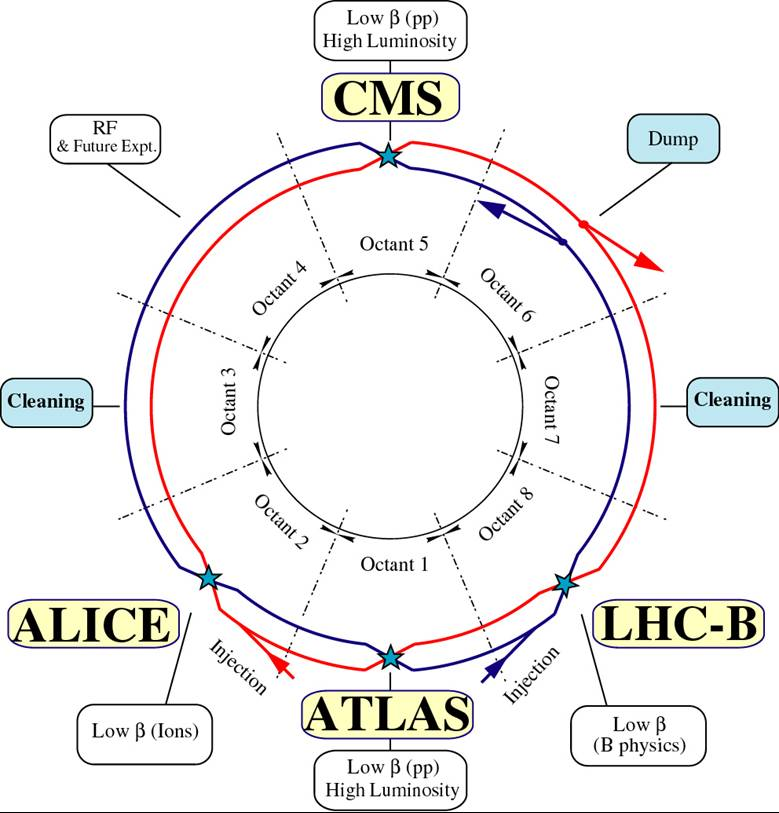
\includegraphics[width=\hsize]{figures/Detector/lhc.jpg}
  \caption{The layout of the LHC and the four detectors along the beam line (ATLAS, LHCb, ALICE, CMS).}. 
  \label{fig:lhc_layout}
\end{figure}
\FloatBarrier


Four sequential particle accelerators are used to accelerate protons from rest as shown in Figure \ref{fig:lhc_accel}. First, Hydrogen gas is ionized to produce protons which are then accelerated to 50 MeV using Linac 2, a linear accelerator. The resulting proton beam is then passed to three circular particle accelerators: Proton Synchrotron Booster, Proton Synchrotron, and Super Proton Synchrotron (SPS), accelerating protons to 1.4, 25, and 450 GeV, respectively. Once the protons exit the SPS, they are injected into the LHC at octant 2 and 8. Each proton bunch contains $\sim 10^{11}$ protons. The spacing between bunches is 25 ns, which means each beam contains 3564 bunches. However, some bunches are left empty due to injection and safety requirements, yielding 2808 bunches per beam. Once the proton beams are injected they are accelerated to 13 TeV. 


\begin{figure}[htbp]
  \centering
  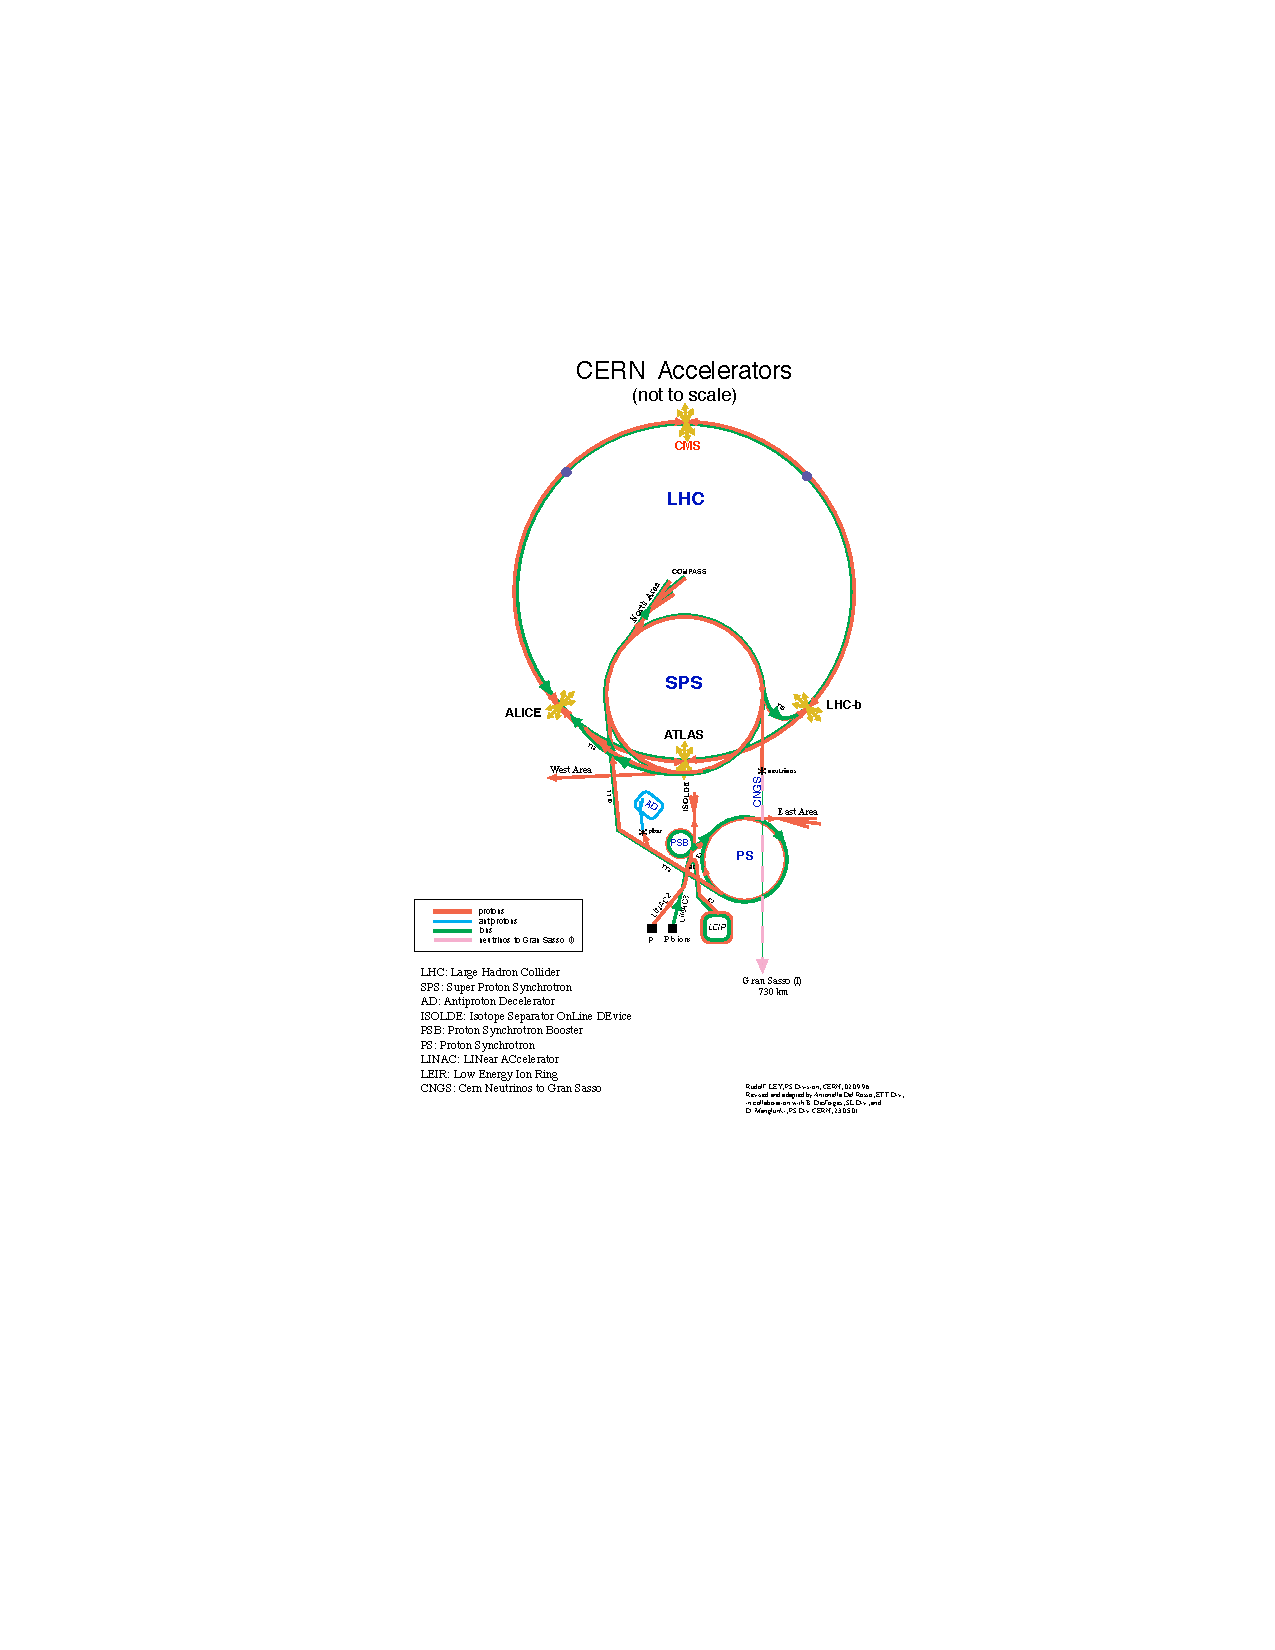
\includegraphics{figures/Detector/lhc_accel.pdf}
  \caption{An overview schematic of the LHC accelerator subsystems.} 
  \label{fig:lhc_accel}
\end{figure}
\FloatBarrier


As many new physics models predict cross-sections below the weak scale it was important to design the LHC to be capable of collecting enough data, by running in high luminosity conditions. The machine luminosity depends only on beam parameters:

\begin{equation}
L=\frac{N_{p}^{2}f}{4\epsilon\beta^{*}}F
\end{equation}

where $N_{p}$ is the number of protons per bunch, f is the bunch crossing frequency, $\epsilon$ is the transverse beam emittance, $\beta^{*}$ is the amplitude function at the collision point, and F is the geometric luminosity reduction factor due to the beams crossing at an angle (rather than head-on). 

\chapter{The ATLAS Detector}
The ATLAS detector measures the position, momentum and energy of particles produced in the proton collisions by using magnetic fields, silicon detectors, sampling calorimeters, and gaseous wire detectors. It is located approximately 100 m underground at Point-1 around the LHC beam line and weighs 7000 metric tons. The detector is 46 m long, 25 m high, 25 m wide  as shown in Figure \ref{fig:atlas_detectors}. The detector can be divided into three subsystems: the Inner Detector (ID), the Calorimeters, and the Muon Spectrometer (MS). Figure \ref{fig:particle_detection} shows an overview of how different particles interact in the detector.
\begin{figure}[h!]
  \centering
  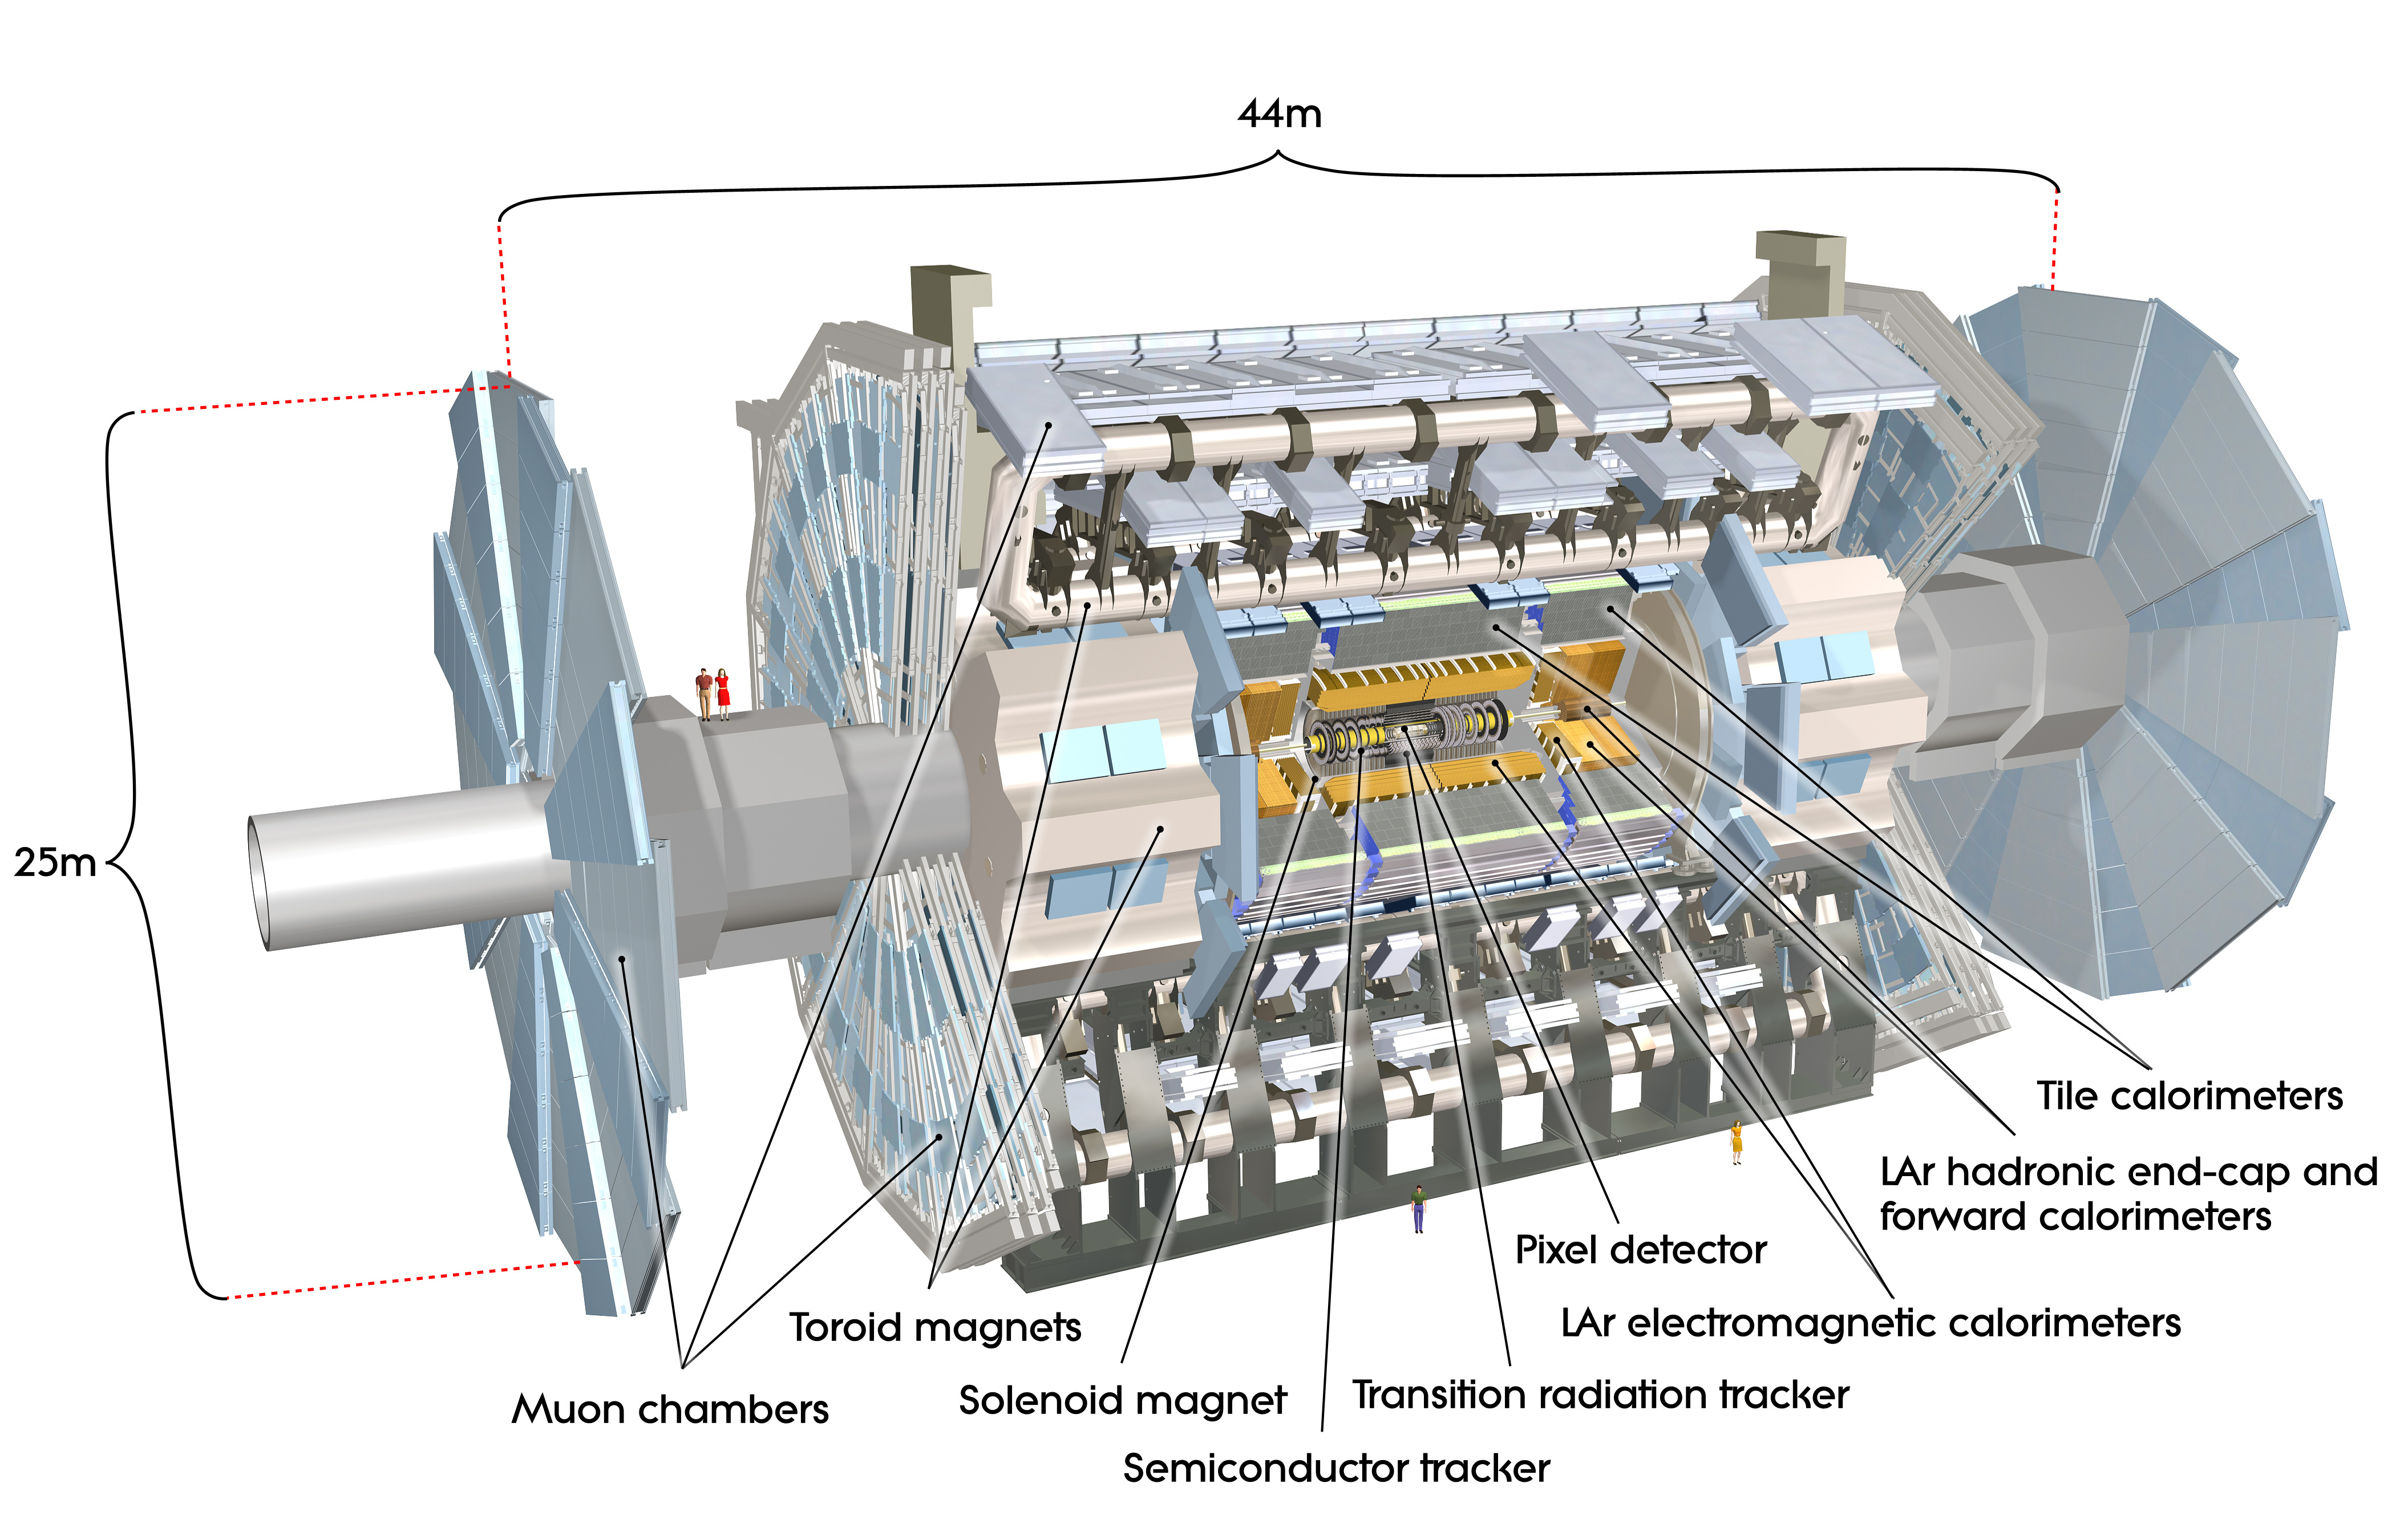
\includegraphics[width=\hsize]{figures/Detector/atlas.jpg}
  \caption{Overview schematic of the ATLAS detector.} 
  \label{fig:atlas_detectors}
\end{figure}
\FloatBarrier


\begin{figure}[h!]
  \centering
  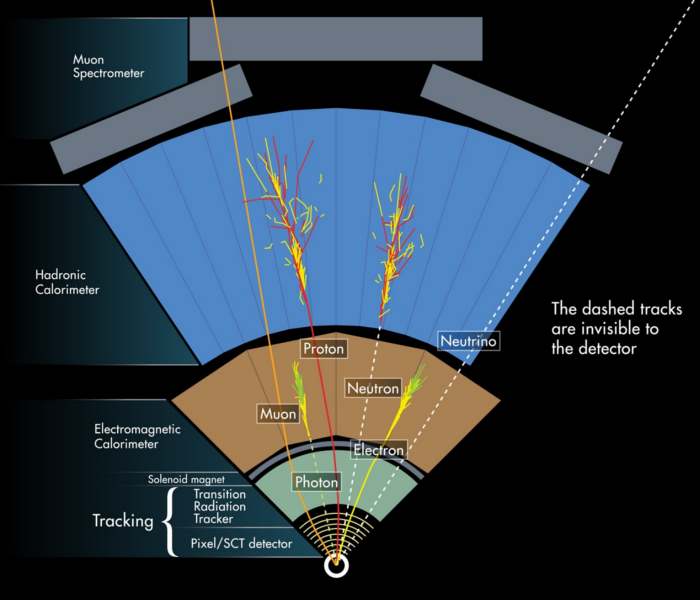
\includegraphics[width=\hsize]{figures/Detector/particle_detection_atlas.png}
  \caption{A simplified schematic of how different particles interact and are detected within ATLAS.} 
  \label{fig:particle_detection}
\end{figure}
\FloatBarrier

\section{Coordinate System}
The trajectory of particles within ATLAS is measured relative to the nominal interaction point. The $z$-axis points along the beam line, such that when the LHC is viewed from above, the counter-clockwise circulating beam points along the positive-$z$ direction. The $x-y$ plane is transverse to the beam line, with the positive x-axis pointing towards the center of the LHC ring. The positive $y$-axis points vertically upward. The azimuthal angle, $\phi$, is the angular distance about the $z$-axis, with $\phi=0$ along the $x$-axis. The polar angle from the $z$-axis is denoted as $\theta$.  However, this quantity is not Lorentz invariant, like rapidity, $y=\frac{1}{2}\ln\frac{E+p_{z}}{E-p_{z}}$, where $E$ is the energy of the particle considered, and $p_{z}$, is it's momentum along the $z$-axis. Pseudorapidity is preferred as $\Delta \eta$ is invariant under boosts along $z$ and particle production is approximately invariant under $\eta$. For massless particles, rapidity and a related quantity, pseudorapidity, are the identical. The pseudorapidity is defined as: $\eta = -\ln \tan(\frac{\theta}{2})$.  This quantity is preferred as it is purely a geometric quantity, independent of particle energy. Angular separation between particles in ATLAS are given by $\Delta R = \sqrt{\Delta \eta^{2}+\Delta \phi^{2}}$. The distance from the beamline is given by $r=\sqrt{x^{2}+y^{2}}$
 
\section{Inner Detector}
The Inner Detector (ID) was designed to identify and reconstruct vertices, distinguish pions from electrons, and measure the momentum of charged particles. The ID uses three different technologies for particle reconstruction: the Pixel Detector, Semiconductor Tracker (SCT), and the Transition Radiation Tracker (TRT), shown in Figure \ref{fig:ID} and \ref{fig:barrelID}. The entire ID is immersed in a 2T solenoidal magnetic field parallel to the $+z$-axis, causing charged particles to bend in the transverse-plane, allowing particle momentum measurements. 

\begin{figure}[h!]
  \centering
  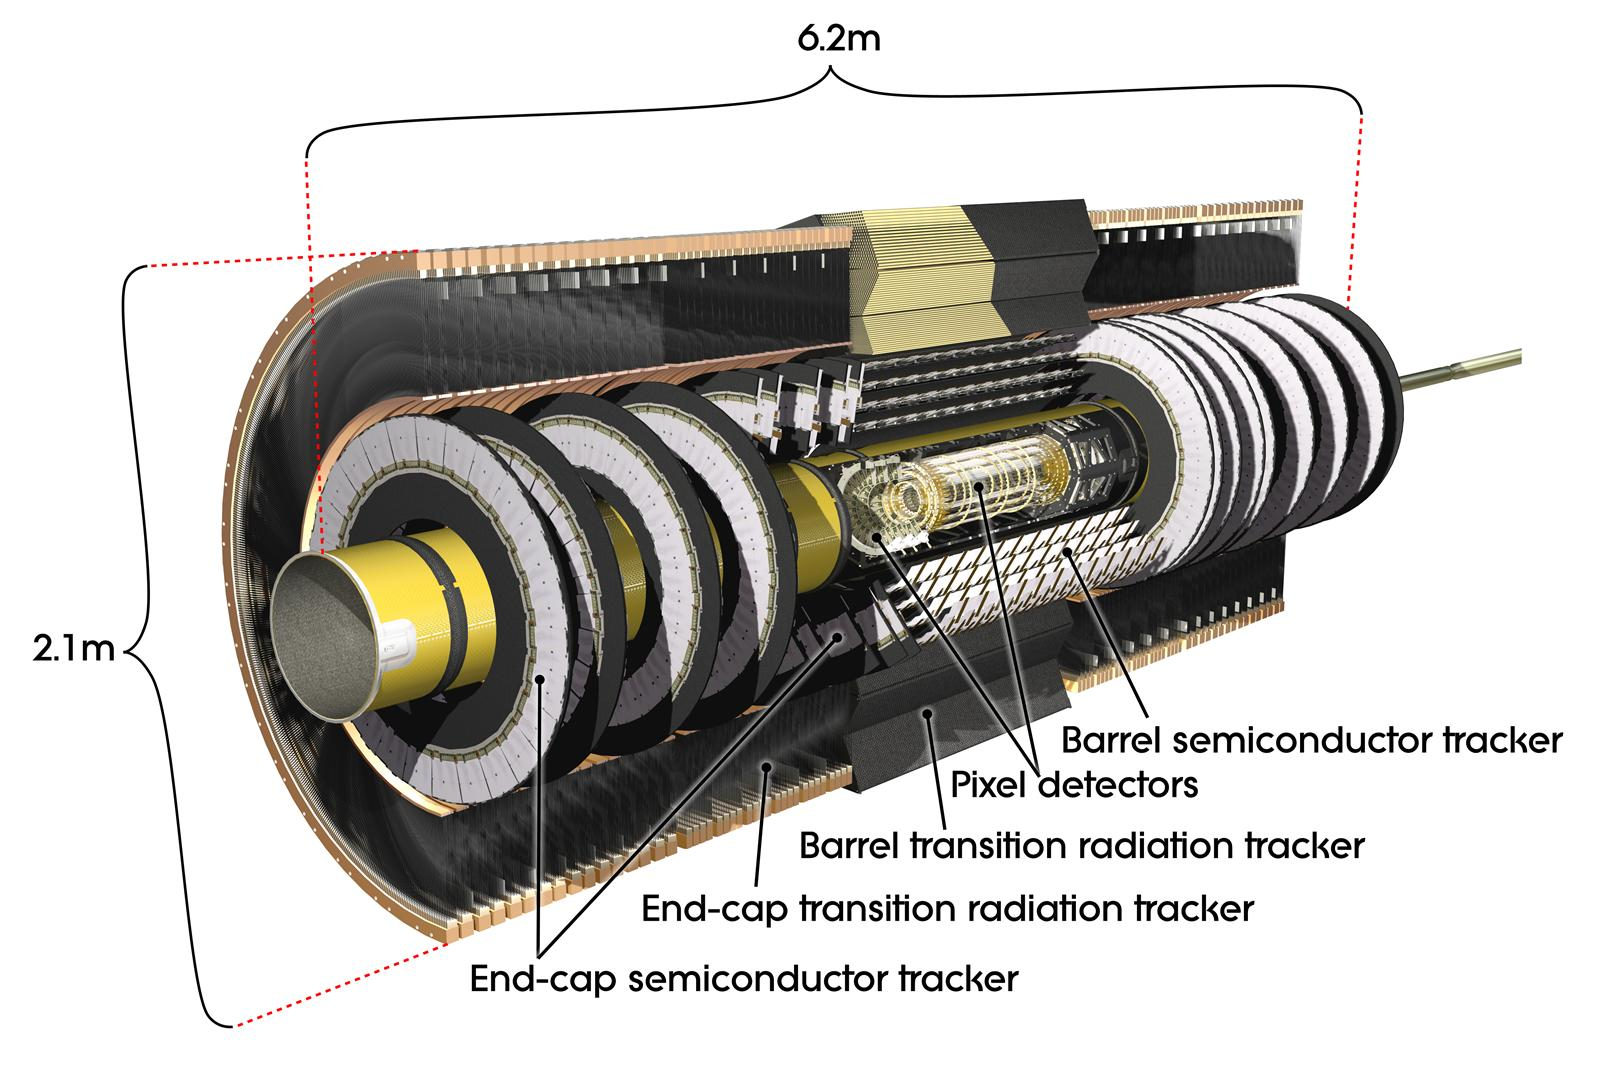
\includegraphics[width=\hsize]{figures/Detector/tracker_layout.jpg}
  \caption{Layout of ATLAS Inner Detector} 
  \label{fig:ID}
\end{figure}
\FloatBarrier


\begin{figure}[h!]
  \centering
  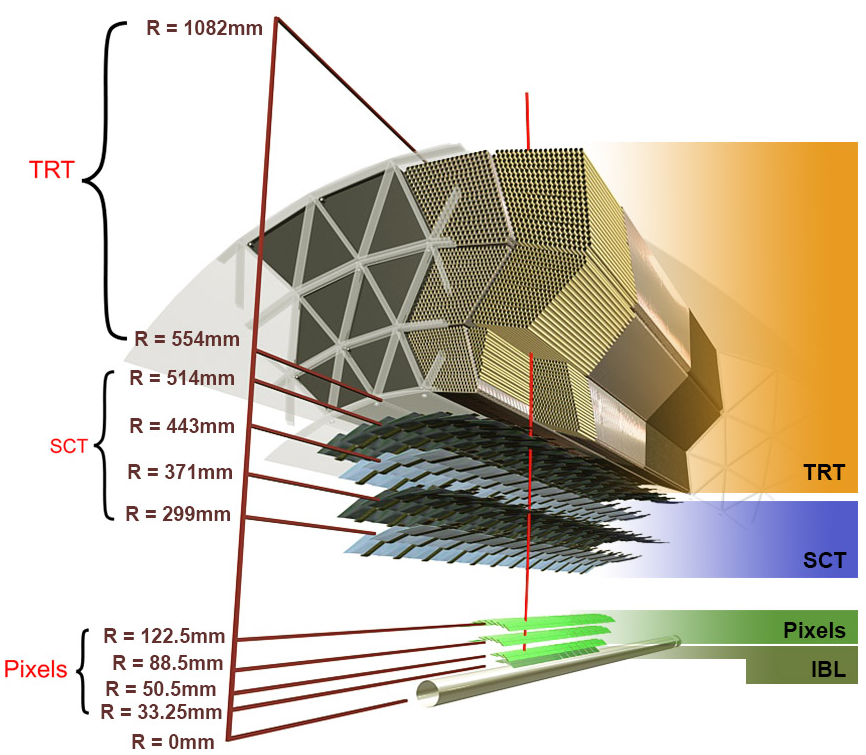
\includegraphics[width=\hsize]{figures/Detector/tracker_barrel.png}
  \caption{Layout of ATLAS ID Barrel System.} 
  \label{fig:barrelID}
\end{figure}
\FloatBarrier


\subsection{Pixel Detector}
The pixel detector consists of four barrel layers between r = 32.7 and 122.5 mm, extending to $|z|=400.5 $mm. The remaining detectors are arranged in barrels and forward and backward rings. The innermost pixel barrel, the Insertable b-Layer (IBL), only extends to $|z|=332$ mm. The pixel detectors closer to the beam line (larger $\eta$ values) consists of six parallel cylindrical rings of pixel detectors transverse to the beam line. The entire pixel detector consists of 1744 identical pixel sensors each with 46080 readout channels, totaling about 80 million individual pixels. Most of the pixel sensors are $50\times400\mu m^{2}$.  Each pixel has a position resolution of 14$\mu$m in $\phi$ and 115 $\mu$m in the $z$ direction.
\subsection{Semiconductor Tracker}
The SCT is located outside the pixel detector and has the same barrel and endcap geometry as the pixel detector. SCT sensors are 80$\mu$m $\times$ 12 cm with a 80$\mu$m strip pitch. In the barrel the strips are parallel to the $z$-axis and are segmented in $\phi$. In the endcaps, the strips extend radially. Sensors are grouped in modules containing two layers of strips rotated 40 mrad with respect to each other. This offset allows for the two-dimensional position of a track to be determined by identifying the crossing point of the strips that registered a hit. SCT modules measure tracks with an accuracy of 17 $\mu$m in $r-\phi$ and 580$\mu$m in $z(r)$ in the barrel (end-cap) region.
\subsection{Transition Radiation Tracker}
The transition radiation tracker (TRT), enveloping the SCT, is a gaseous straw-tube tracker mainly used for electron/pion track separation. Each straw is 4 mm in diameter and filled with a Xe-C$O_{2}$-$O_{2}$ gas mixture. An anode wire at the center of the straw is held at ground potential, while the walls of the straw are kept at -1.4kV. When a charged particle passing through the TRT ionizes the gaseous mixture, the resulting ions form an avalanche on the anode wire with a gain of $\sim 10^{4}$. The signal from the anode wire is then digitized and discriminated. Signals passing a low threshold cutoff are used to distinguish noise from tracks. Signals passing a high threshold cutoff are sensitive to transition radiation (TR). TR photons are emitted when charged particles pass between materials with different dielectric constants. The probability that a charged particle with energy $E$ and mass $m$ passing between two materials emits a TR photon in the keV range is proportional to $\gamma=E/m$. In the TRT staws these often then convert via the photoelectric effect, causing a large avalanche triggering the high-threshold. Since electrons have a smaller mass than pions, electron tracks are more likely to trigger the high threshold. This then provides discrimination between electrons and charged hadrons.

The barrel region of the TRT extends from $r=$563-1066 mm and $|z| < 712$ mm. Barrel Straws are 144 cm long (divided  $\sim \eta \approx 0$) and orientated parallel to the beam direction. End-cap straws extend radially and are 37 cm long. There are 53,544 straws in the barrel and 160,000 straws in the end-caps. Radiator mats of polypropylene/polyethylene fibers in the barrel are aligned perpendicular to the barrel straws (with holes for the straws to pass through). In the end-cap region, radiator foils are layered between the radial TRT straws. 

The arrival time of the signal pulse is sensitive to the distance between the charged particle track and the anode wire and allows for a hit resolution of 130$\mu$m. The TRT extends to $|\eta| = 2.0$ and provides about 36 hits per track.
\section{Calorimeters}
The ATLAS electromagnetic and hadronic calorimeters (EMC and HCAL, respectively) absorb and measure the energy of high energy hadrons, photons, and electrons with $|\eta| < 4.9$. Both systems use sampling calorimeters which consist of alternating layers of dense absorbing and active layers. In the absorbing layer particles interact and lose energy, creating showers. These showers are then detected and measured in the active layer. The amount of charge measured in the active material scales with the energy of the incident particle, and thus provides a measurement of the particle's energy. An overview of the layout of the calorimeter system is shown in Figure \ref{fig:calo_overview}.

The EMC measures and contains the energy of electromagnetically interacting particles. It consists of layered accordion-shaped Lead absorber plates and electrodes immersed in liquid Argon with 170k channels.. Using accordion-shaped electrode and absorbers ensures $\phi$ symmetry and coverage. The EMC is composed of a barrel part ($|\eta| < 1.475$), two end-caps ($1.375<|\eta| < 3.2$), and a presampler ($|\eta| < 1.8$).  The presampler, containing only liquid Argon, corrects for upstream energy losses of electrons and photons. The EMC barrel is segmented into three layers. The first layer has finest segmentation with readout cells extending $\Delta \eta \times \Delta \phi = 0.025/8 \times 0.1$. This provides a precise shower measurements used to separate prompt photons from $\pi^{0} \rightarrow \gamma \gamma$ decays. The second layer has coarser segmentation and is approximately 16 radiation lengths long. A radiation length is the average distance an electron travels before losing all but 1/$e$ of its energy to bremsstrahlung. The last layer is the most coarse and measures the tail of the electromagnetic shower. A schematic of the ECAL is shown in Figure \ref{fig:ecal}. 

The hadronic calorimeter located outside the EMC and is used to contain and measure the energy of hadronically interacting particles. It consists of a tile calorimeter (TileCal), hadronic end-cap calorimeter (HEC), and liquid Argon forward calorimeter (FCAL). TileCal is located behind the LAr EMC and uses steel absorbers and liquid Argon as the active material. TileCal consists of three barrel layers in the central and forward regions, extending up to $|\eta| < 1.7$. Photons generated from hadronic interactions are collected via wavelength-shifting fibers connected to photomultiplier tubes, as shown in Figure ~\ref{fig:hcal}. The HEC lies behind the EMC endcap wheels. It uses copper absorbers and liquid Argon as the active material and covers $1.5 < |\eta| < 3.2$. Finally, the FCAL covers $3.1 < |\eta| < 4.9$ and consists of three modules all using liquid Argon as the active material. The first module uses copper absorber and was designed for electromagnetic measurements. The second and third modules consist of tungsten absorber and are used to measure the kinematics of hadronically interacting particles. A schematic of the HCAL is shown in Figure \ref{fig:hcal}. 

\begin{figure}[h!]
  \centering
  \includegraphics[width=\hsize]{figures/Detector/calo_overview.pdf}
  \caption{Overview of ATLAS electromagnetic and hadronic calorimeters.} 
  \label{fig:calo_overview}
\end{figure}
\FloatBarrier


\begin{figure}[h!]
  \centering
  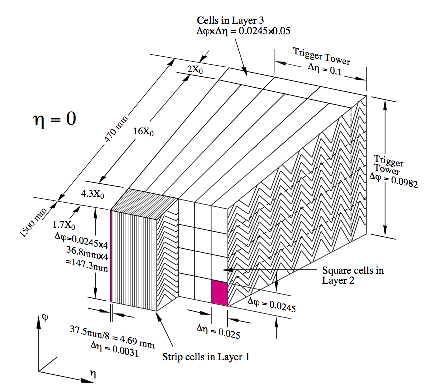
\includegraphics[width=\hsize]{figures/Detector/ecal.pdf}
  \caption{Schematic of ECAL.} 
  \label{fig:ecal}
\end{figure}
\FloatBarrier




\begin{figure}[h!]
  \centering
  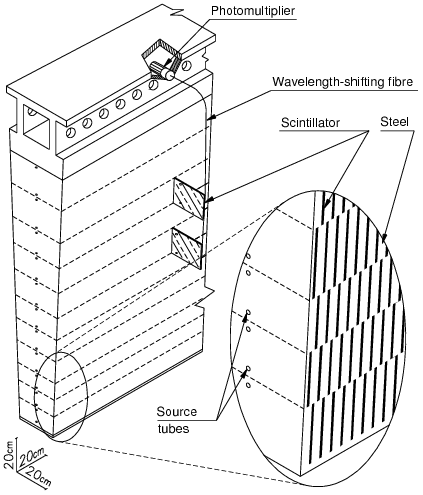
\includegraphics[width=\hsize]{figures/Detector/hcal.png}
  \caption{Schematic of HCAL.} 
  \label{fig:hcal}
\end{figure}
\FloatBarrier


The energy resolution of the calorimeter subsystems are:

$\frac{\sigma_{E}}{E}=\frac{10\%}{\sqrt{E}}\bigoplus \frac{0.3\%}{E}\bigoplus 0.4\%$ Electromagnetic Calorimeter

$\frac{\sigma_{E}}{E}=\frac{50\%}{\sqrt{E}}\bigoplus \frac{1.8\%}{E}\bigoplus 3\%$ Hadronic Calorimeter


\section{Muon Spectrometer}
The muon spectrometer (MS) is the outermost detector system in ATLAS. Muons with a $p_{T}>4$ GeV are energetic enough to reach the MS. To measure the momentum of these muons barrel and end-cap toroid magnets are used covering $|\eta| < 1.4$ and $1.6<|\eta|<2.7$. For $1.4 < |\eta| < 1.6$, a combination of the barrel and end-cap toroidal magnetic fields bend muon trajectories. The detector in the barrel region form three concentric rings at $R=5, 7.5, 10$ m and are segmented in $\phi$ to accommodate the magnets. The end-cap region consists of three circular planes perpendicular to $z$ and located at $|z|=7.4, 14, 21.5$ m from the interaction region. An additional detector at $|z|=10.8$ m covers the transition region between the barrel and end-cap.

The MS readout consists of four subsystems: Monitored Drift Tubes (MDT), Cathode Strip Chambers (CSC), Resistive Plate Chambers (RPC), and Thin Gap Chambers (TGC). The first two subsystems are used primarily for measuring muon track parameters, while the RPC and TGC subsystems are used for muon triggering. A schematic of this system is shown in Figure ~\ref{fig:muonsys}. 

The MDT subsystem consists of precision tracking chambers for $|\eta|<2.7$, except for the inner most end-cap layer ($2.0 < |\eta| < 2.7$), where CSCs are used. The basic unit of MDT chambers are thin walled Aluminum tubes with a diameter of 3 cm and length of 0.9-6.2 m. These tubes are filled with a mixture of Ar-CO$_{2}$ gas with a  50$\mu$m W-Rn wire running down the center of the tube, which is kept at 3080 V. Since the maximum drift time of these chambers is $\sim$ 700 ns, they are not used for triggering. MDT chambers consist of 3-4 layers of tubes mounted on a rectangular support system, as seen in Figure ~\ref{fig:muon_mdt}, orientated along $\phi$ to measure the coordinate in the bending plane of the magnetic field with a resolution of 35 $\mu$m.

The MDT subsystem can only handle hit rates below 150 Hz/cm$^{2}$. For this reason, CSCs are used in the innermost end-cap layer where hit rates are larger. CSCs can handle hit rates up to 1000Hz/cm$^{2}$. CSC are multiwire proportional chambers. These chambers are filled with a Ar-C$O_{2}$ gas mixture and evenly spaced wires kept at 1900 V. These wires are orientated in the radial direction but not read out. Instead on one side of the cathode are copper strips parallel to the wires, measuring $\eta$, while on the other side of the cathode are strips parallel to the wires measuring $\phi$. The width between strips is approximately 1.5 mm providing a resolution of 60 $\mu$m in the bending-plane and 5 mm in the non-bending plane. 

Since the CSC and MDT systems do not have prompt timing signals, the RPC and TGC systems are used for triggering. The RPC system is used in the barrel region ($|\eta| < 1.05$). RPC consist of two parallel resistive plates separated by a 2 mm insulated spacer with 100 mm spacing kept at 9.8 kV, as shown in Figure \ref{fig:muon_rpc}. A gaseous mixture of C$_{2}$H$_{2}$F$_{4}$, C$_{4}$H$_{10}$, and SF$_{6}$ fills the space between the two plates. Metallic strips on the outer faces of the plates are used to read out signals produced by the gas ionizing. The middle barrel layer consists of two layers of RPCs on either side of the MDT layer and one layer on the outermost MDT layer. Each layer contains two orthogonal sets of metallic strips providing $\eta$ and $\phi$ measurements. The timing resolution of RPCs is 1.5 ns, and therefore may be used to identify bunch crossings. 

Finally, the TGCs are used in the end-cap regions and are primarily used to provide L1 trigger decisions and $\phi$ measurements. TGCs are multi-wire proportional chambers consisting of arrays of gold-coated tungsten wires placed between two cathode planes. These wires are separated by 1.8 mm and cathodes are 1.4 mm from the wires. Orthogonal to the wires, on the opposite side of the cathode plane are copper strips held at 2900 V. The chambers are filled with a mixture of CO$_{2}$ and n-pentane gas, the latter acts as a quenching gas to prevent avalanches initiated by secondary $\gamma$-rays from the primary avalanche. Figure ~\ref{fig:muon_tgc} is a schematic of a TGC. The timing resolution of TGCs is less than 25 ns and therefore they are used for bunch crossing measurements. 

\begin{figure}[h!]
  \centering
  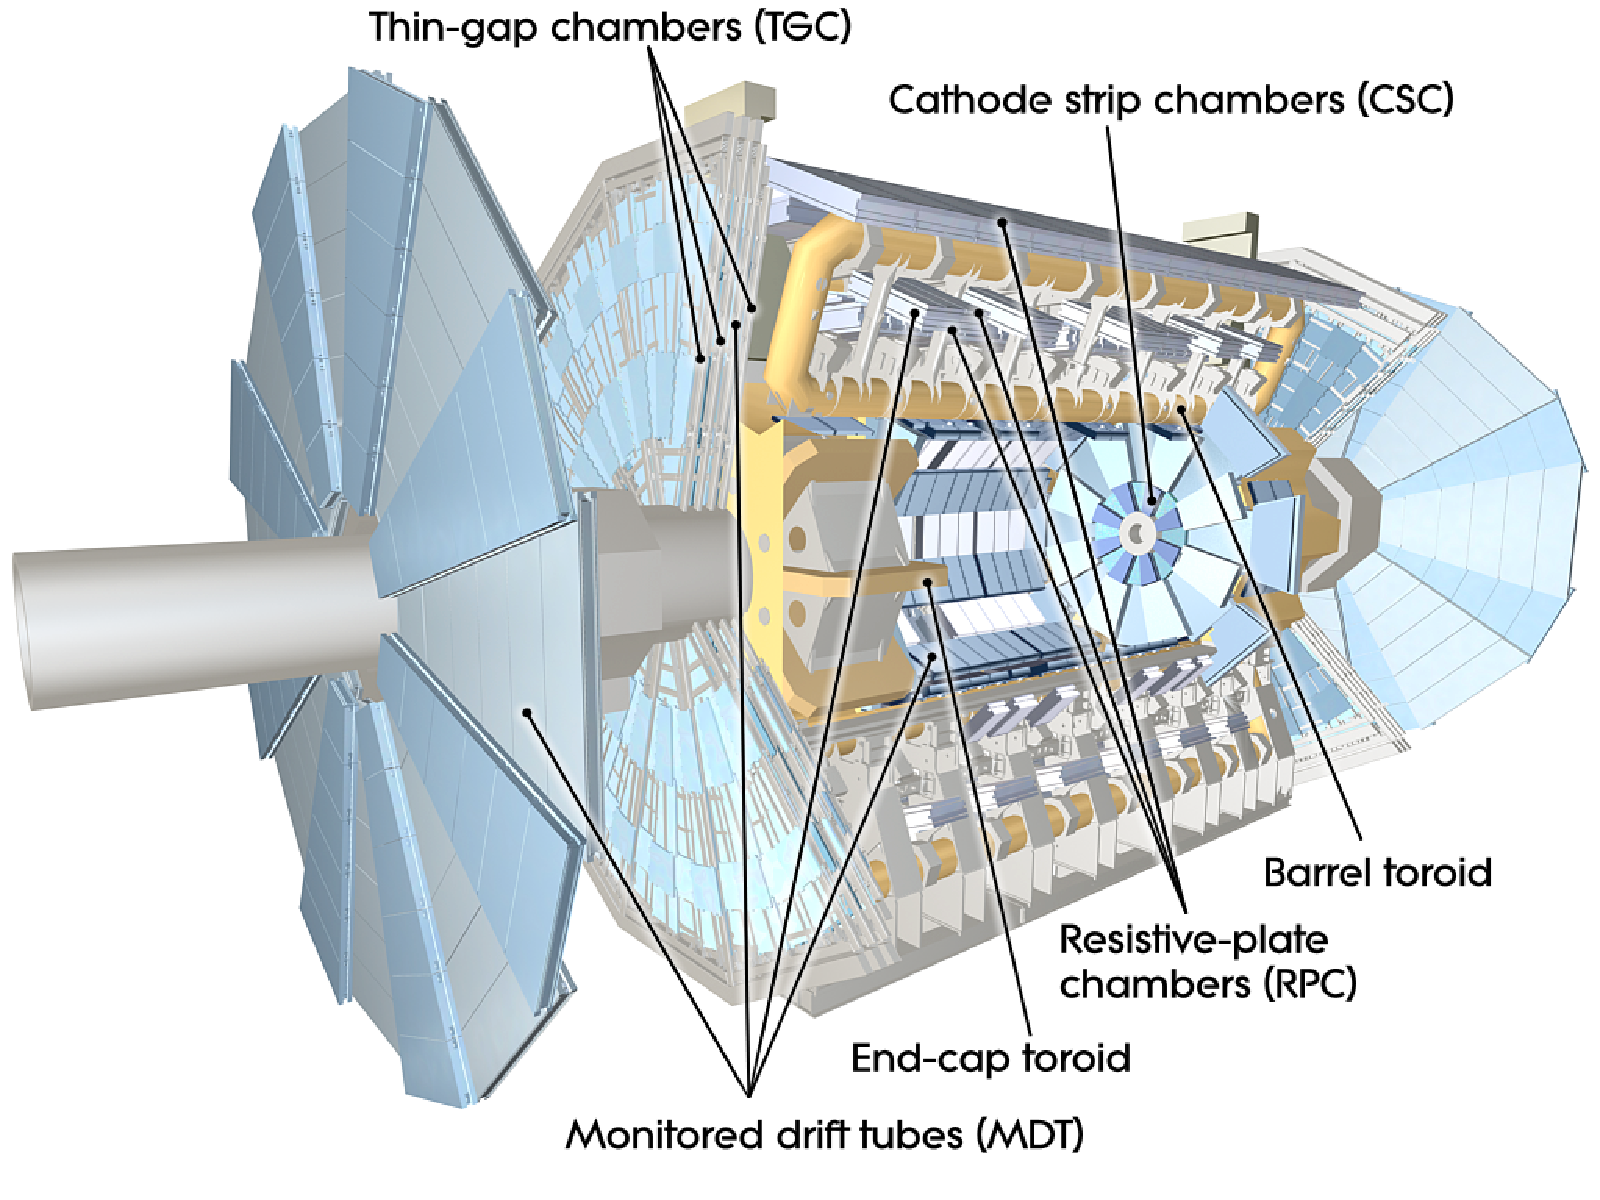
\includegraphics[width=\hsize]{figures/Detector/muonsys.pdf}
  \caption{Schematic of Muon Spectrometer [cite G35]} 
  \label{fig:muonsys}
\end{figure}
\FloatBarrier


\begin{figure}[h!]
  \centering
  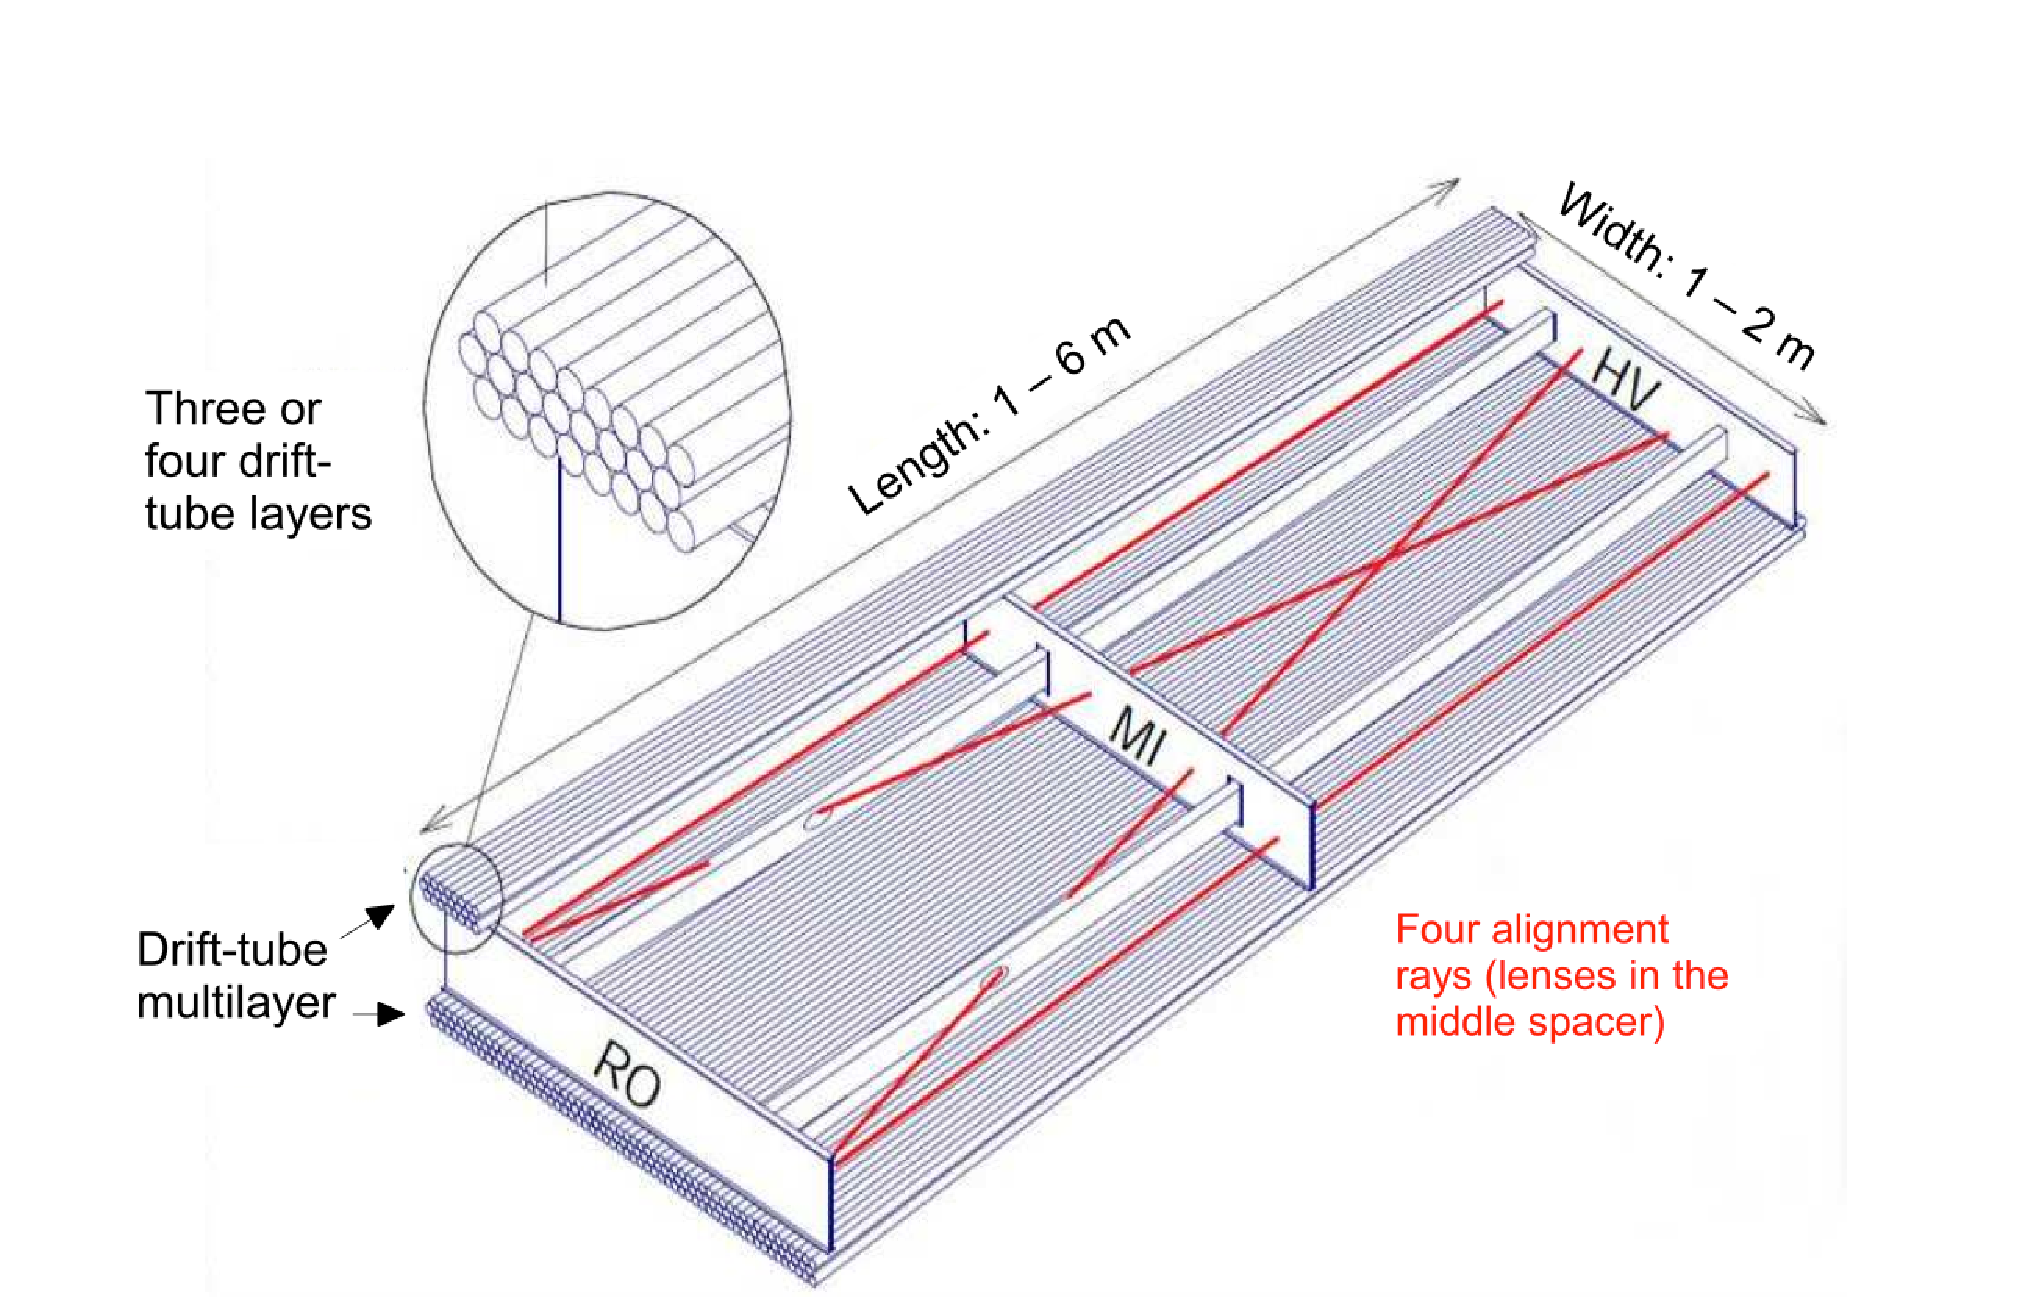
\includegraphics[width=\hsize]{figures/Detector/muon_mdt.pdf}
  \caption{Schematic of MDT chamber. [cite G35]} 
  \label{fig:muon_mdt}
\end{figure}
\FloatBarrier


\begin{figure}[h!]
  \centering
  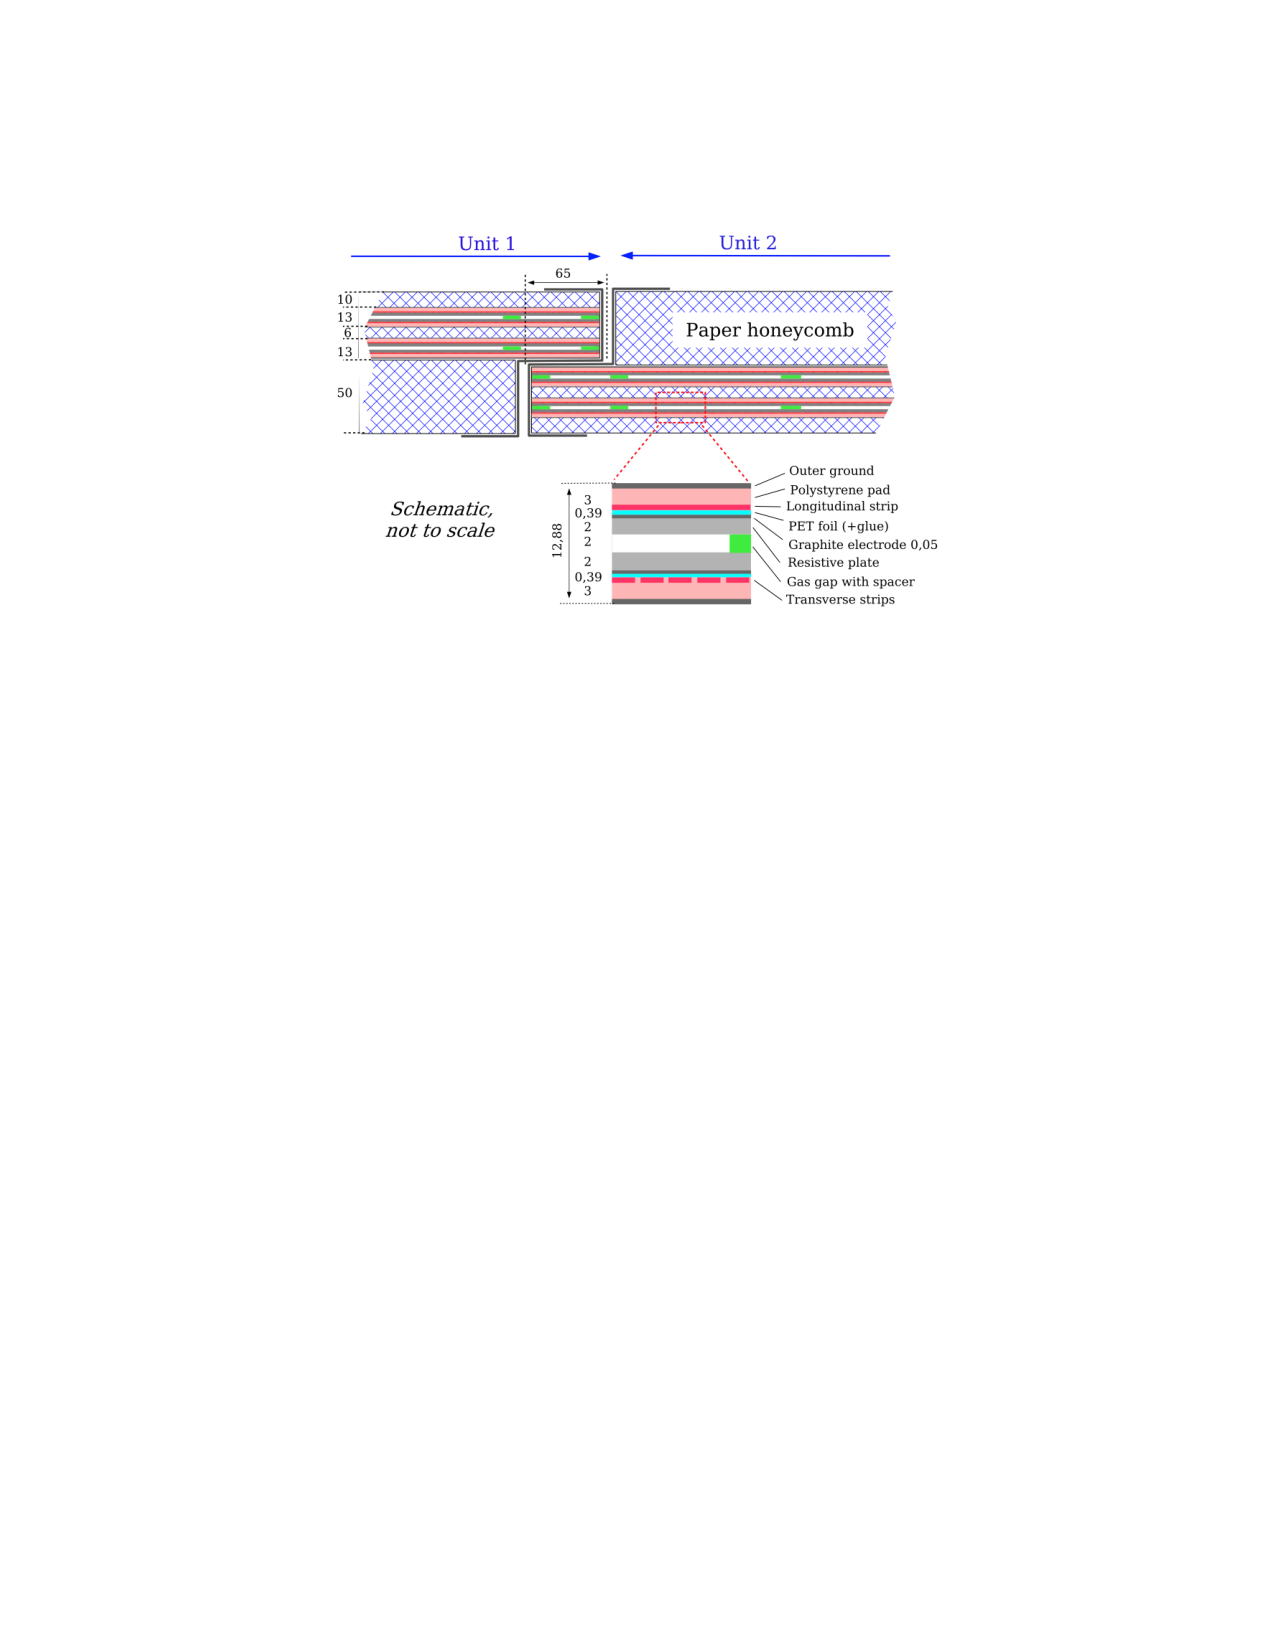
\includegraphics[width=\hsize]{figures/Detector/muon_rpc.pdf}
  \caption{Schematic of RPC chamber, which is used for triggering in the central region of the detector [cite G35].} 
  \label{fig:muon_rpc}
\end{figure}
\FloatBarrier



\begin{figure}[h!]
  \centering
  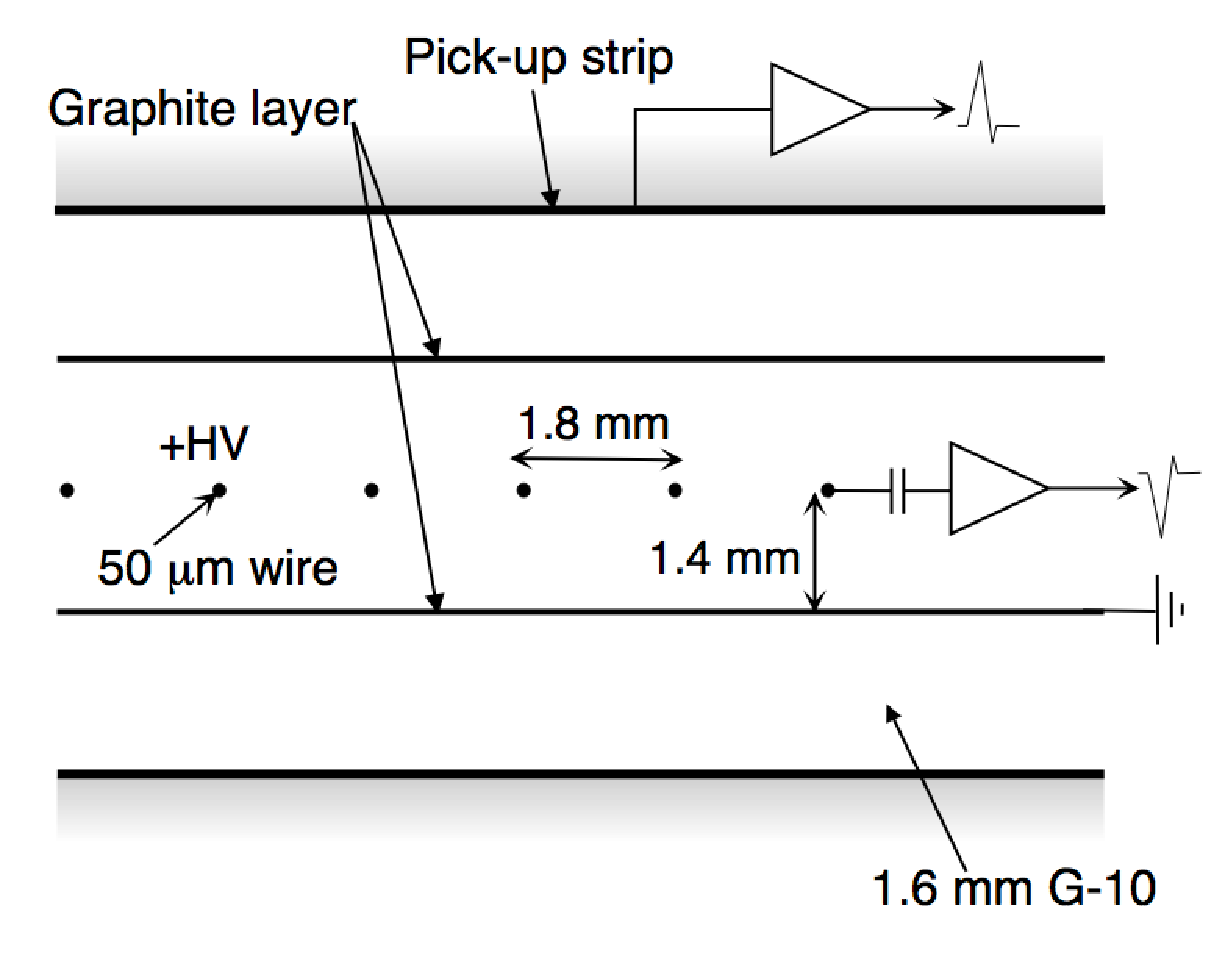
\includegraphics[width=\hsize]{figures/Detector/muon_tgc.pdf}
  \caption{Schematic of TGC chamber, which is used for triggering in the muon end-cap region. [cite G35]} 
  \label{fig:muon_tgc}
\end{figure}
\FloatBarrier

\section{Magnet System}
A particles with charge, q, and velocity v, moving in magnetic field, B, experiences a force, $F= qv\times B$. This force can cause charged particles to have a curved trajectory in magnetic fields, which the ID and MS use to determine the particles $p_{T}$. The central solenoid provides the magnetic field for the ID and the toroidal magnets provide the magnetic field for the MS.

The layout of the magnet system is shown in Figure \ref{fig:atlas_magnets}. The central solenoid consists of a single-layer Al-stabilized NbTi conductor coil wound inside an Al support cylinder. The solenoid is 5.8 m long, 50 cm thick and has an inner radius of 1.23 m. It is cooled to 4.5 K to reach superconducting temperatures and shares the liquid argon calorimeter vacuum vessel to minimize material in the detector. A current of 7.730 kA produces a 1.998 T solenoidal magnetic field, pointing in the +$z$ direction. 

The toroidal magnet system consists of a barrel and two end-cap toroidal magnets used to create a magnetic field outside the calorimeters that is orientated along $\phi$. Each barrel toroid is 25.3 m long with an inner and outer diameter of 9.4 and 20.1 m and weighs 830 tonnes. Endcap toroids are 5 m long with an inner and outer radius of 1.65 and 10.7 m. Both toroid systems use Al-stabilized Nb/Ti/Cu conductors. The magnetic field strength in the barrel and endcap regions are 0.5 and 1 T, respectively.

\begin{figure}[h!]
  \centering
  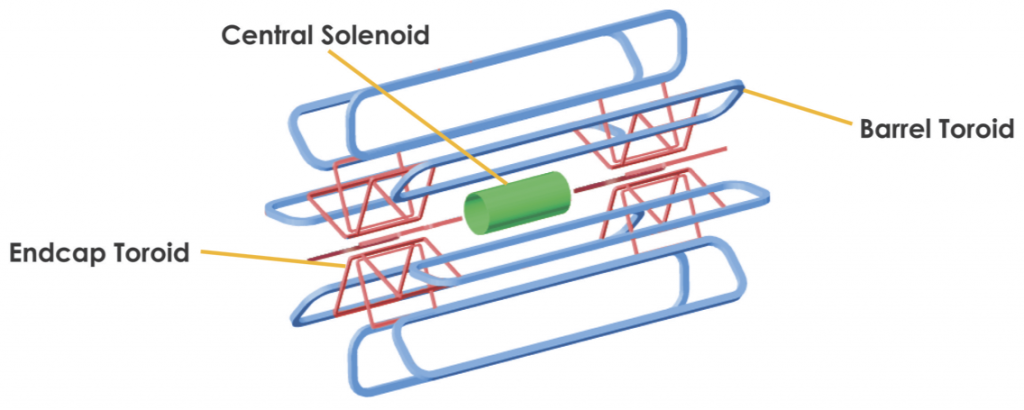
\includegraphics[width=\hsize]{figures/Detector/atlas_magnets.png}
  \caption{Layout of ATLAS magnet systems.} 
  \label{fig:atlas_magnets}
\end{figure}
\FloatBarrier


\section{Trigger System}
Since collisions occur every 25 ns and reading out all detector channels and storing that information is not currently feasible (would require saving 60 million megabytes per second), the majority of events are not kept for analysis. ATLAS uses a multi-stage trigger system to select approximately 1,000 of the 1.7 billion collisions that occur each second (corresponding to a rate of 1 kHz from the 40 MHz proton collision rate). The first stage of the trigger system is the hardware level (L1) trigger. This trigger reduces the event rate to $\sim$100 kHz by identifying Regions-of-Interest (ROIs) containing high $p_{T}$ leptons, photons, jets, or $E_{T}^{miss}$ by using information from RPCs, TGCs, and calorimeters to make a 2.5 $\mu$s decision. This information is then passed to a high-level trigger (HLT) which further decreases event rates to $\sim$ 1 kHz. The HLT uses finer granularity measurements from the MS and ID to preform simplified offline reconstruction to decide which events to keep.


\part{Method}
\label{ch:analysis}
\chapter{Dataset and Simulated Samples}
\section{Dataset}
This analysis uses $pp$ collision data collected from 2015 to 2018 at $\sqrt{s}=13$ TeV, corresponding to 139/fb of data as shown in Figure \ref{fig:int_lumi} and \ref{fig:mu_profile}. From this dataset, only those events in which the tracker, calorimeters, and muon spectrometer have good data quality are used.  For a given event, the solenoid and toroidal magnets must also be operating at their nominal field strengths. In addition to this, events must pass further quality checks to reject events where detector subsystems may have failed. These selections reject events that containing LAr noise bursts, saturation in the electromagnetic calorimeter, TileCal errors, and failures in event recovery due to tracker failures. Events with information missing from subsystems (usually due to busy detector conditions) are rejected.  Events must also contain a primary vertex with at least two associated tracks, where the primary vertex is selected as the vertex with the largest $\sum p_{T}^{2}$ over tracks associated with the vertex and $p_{T}>0.5$ GeV.


\begin{figure}[h!]
  \centering
  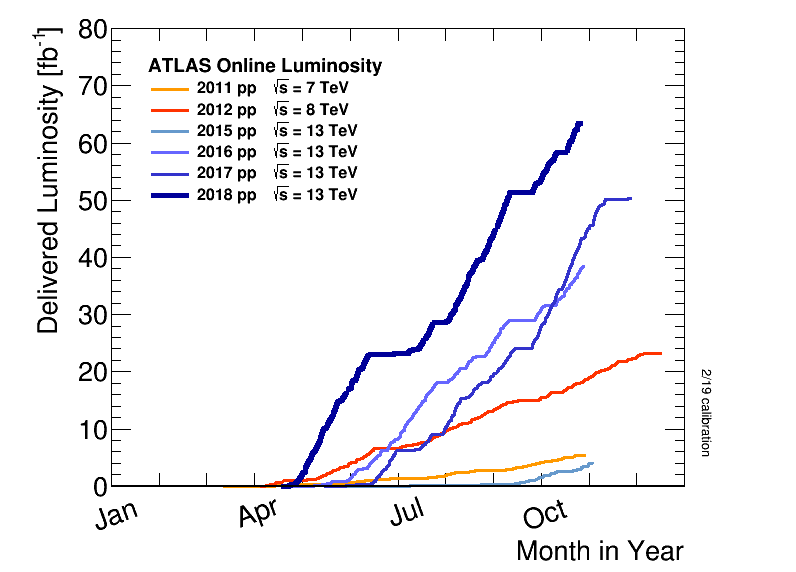
\includegraphics[width=\hsize]{figures/Analysis/lumi.png}
  \caption{Integrated luminosity for data collected from ATLAS from 2011 - 2018}. 
  \label{fig:int_lumi}
\end{figure} 
\FloatBarrier

\begin{figure}[h!]
  \centering
  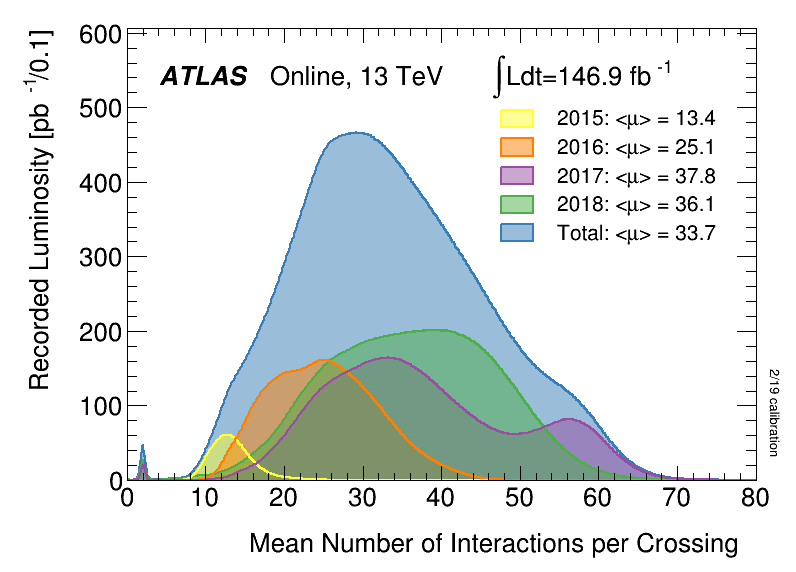
\includegraphics[width=\hsize]{figures/Analysis/mu_profile.png}
  \caption{Mean number of interactions per crossing for data collected from ATLAS from 2011 - 2018}. 
  \label{fig:mu_profile}
\end{figure} 
\FloatBarrier


\section{Simulated Samples}
\label{Simulated Samples}
Samples are simulated in order to model backgrounds, evaluate signal acceptance, optimize event selection and estimate systematic and statistical uncertainties. The dominant backgrounds for this analysis are $W/Z$ + jets, diboson ($WZ$/$WW$), $t\bar{t}$, single top and multijet production. 

$W/Z$+jet events are simulated using Sherpa 2.2.1 at NLO \cite{sherpa} and merged with the Sherpa parton shower using the ME+PS@NLO prescription \cite{me_ps}. These events are then normalized to NNLO cross sections. The $t\bar{t}$ and single-top backgrounds are generated with Powheg-Box with NNPDF3.0NLO PDF sets in the matrix element calculation \cite{pdfsets}. For all processes, the parton shower, fragmentation, and underlying event are simulated using Pythia 8.320 with the A14 tune set \cite{pdfsets}. Diboson processes are generated using Sherpa 2.2.1. 

Signal samples are simulated using MadGraph 5-2.2.2 \cite{nnlo} and Pythia 8.186 with NNPDF230LO. RS Graviton samples are generated with $k/M_{PL}$=1. HVT Model A (B) samples are simulated with $g_{V}=1(3)$, as the difference in the width of the samples is smaller than detector resolution. To model VBF production of HVT signals, $g_{H}=1$ and $g_{f}=0$. Signals are generated for masses between 300 GeV and 5 TeV.

\chapter{Objects}
\section{Electrons}
Electrons are reconstructed from electromagnetic showers in the LAr EM calorimeter. During reconstruction cells of $\Delta \eta \times \Delta \phi = 0.025 \times 0.025 $ are grouped into 3$\times$5 clusters. These clusters are then scanned for local maxima that seed electron clusters. These clusters must then be matched to ID track from the PV. This requirement minimizes non-prompt electron and fake electron backgrounds. Electrons must pass identification and isolation requirements. Electron identification (loose, medium, tight) classification is based on a multivariate discriminant that identifies electrons using a likelihood based method. For this analysis, events are required to have one tight electron and no additional loose electrons. Electrons are also required to be isolated. The electrons are considered isolated if the quotient of the sum of the transverse momentum (of calorimeter energy deposits) in a cone around the electron of size $\Delta R = 0.2$ and the transverse momentum of the electron to be less than $0.015*p_{T}$ or 3.5 GeV, whichever is smaller. This requirement rejects non-prompt photons and other fake leptons. Electrons in this analysis are also required to have $p_{T} > 30$ GeV and $|\eta| < 2.47$. Electrons are also required to have $p_{T} > 30$ GeV.

Electrons are calibrated to determine data-driven scale factors using $J/ \Psi \rightarrow ee$, $Z \rightarrow ee$, $Z \rightarrow \ell \ell \gamma$ processes. These corrections account for the  non-uniform response of the detector which introduces modeling and reconstruction uncertainties. 

\section{Muons}
As muons traverse the entire detector, they are reconstructed from ID and MS tracks. For this analysis the muon identification and isolation working points are chosen to minimize the contributions from non-prompt muons. Towards this end, each selected event must contain exactly one muon that passes the medium identification working point, and no additional muons (that pass the loose working point). For the medium working point, two types of reconstructed muons are used: combined and extrapolated muons (CB and ME, respectively). For CB muons, ID and MS tracks are reconstructed independently and a combined track fit is performed by adding or removing MS tracks to improve the fit quality. ME muons are reconstructed from only MS tracks with hits in at least two layers, which ensures the track originates from the PV. ME muons extend the acceptance for muon reconstruction outside the ID from $2.5 < |\eta| < 2.7$.
The medium identification working point uses CB and ME tracks. CB tracks must have at least 3 hits in two MDT layers. ME tracks are required to have at least three MDT/CSC hits. To further minimize contributions from fake muons, the selected muons are required to be isolated from other tracks, as muons from $W,Z$ decays are often isolated from other particles. To insure the selected muons are isolated, the scalar sum of the transverse momentum of tracks in a cone of $\Delta R = 0.3$ compared to the transverse momentum of the muon must be less then 0.06. Muons are also required to have $p_{T} > 30$ GeV.

Muons are calibrated using well-studied resonances $J/ \Psi \rightarrow \mu \mu$ (for $p_{T}^{\mu}< 10$ GeV),  $Z \rightarrow \mu \mu$ (for $p_{T}^{\mu} > 10$ GeV). Figure \ref{fig:muon_syst} shows the combined muon $p_{T}$ uncertainty from this calibration. The total systematic uncertainty is less then 1\% for all $p_{T}$ ranges considered in this analysis.


\begin{figure}[h!]
  \centering
  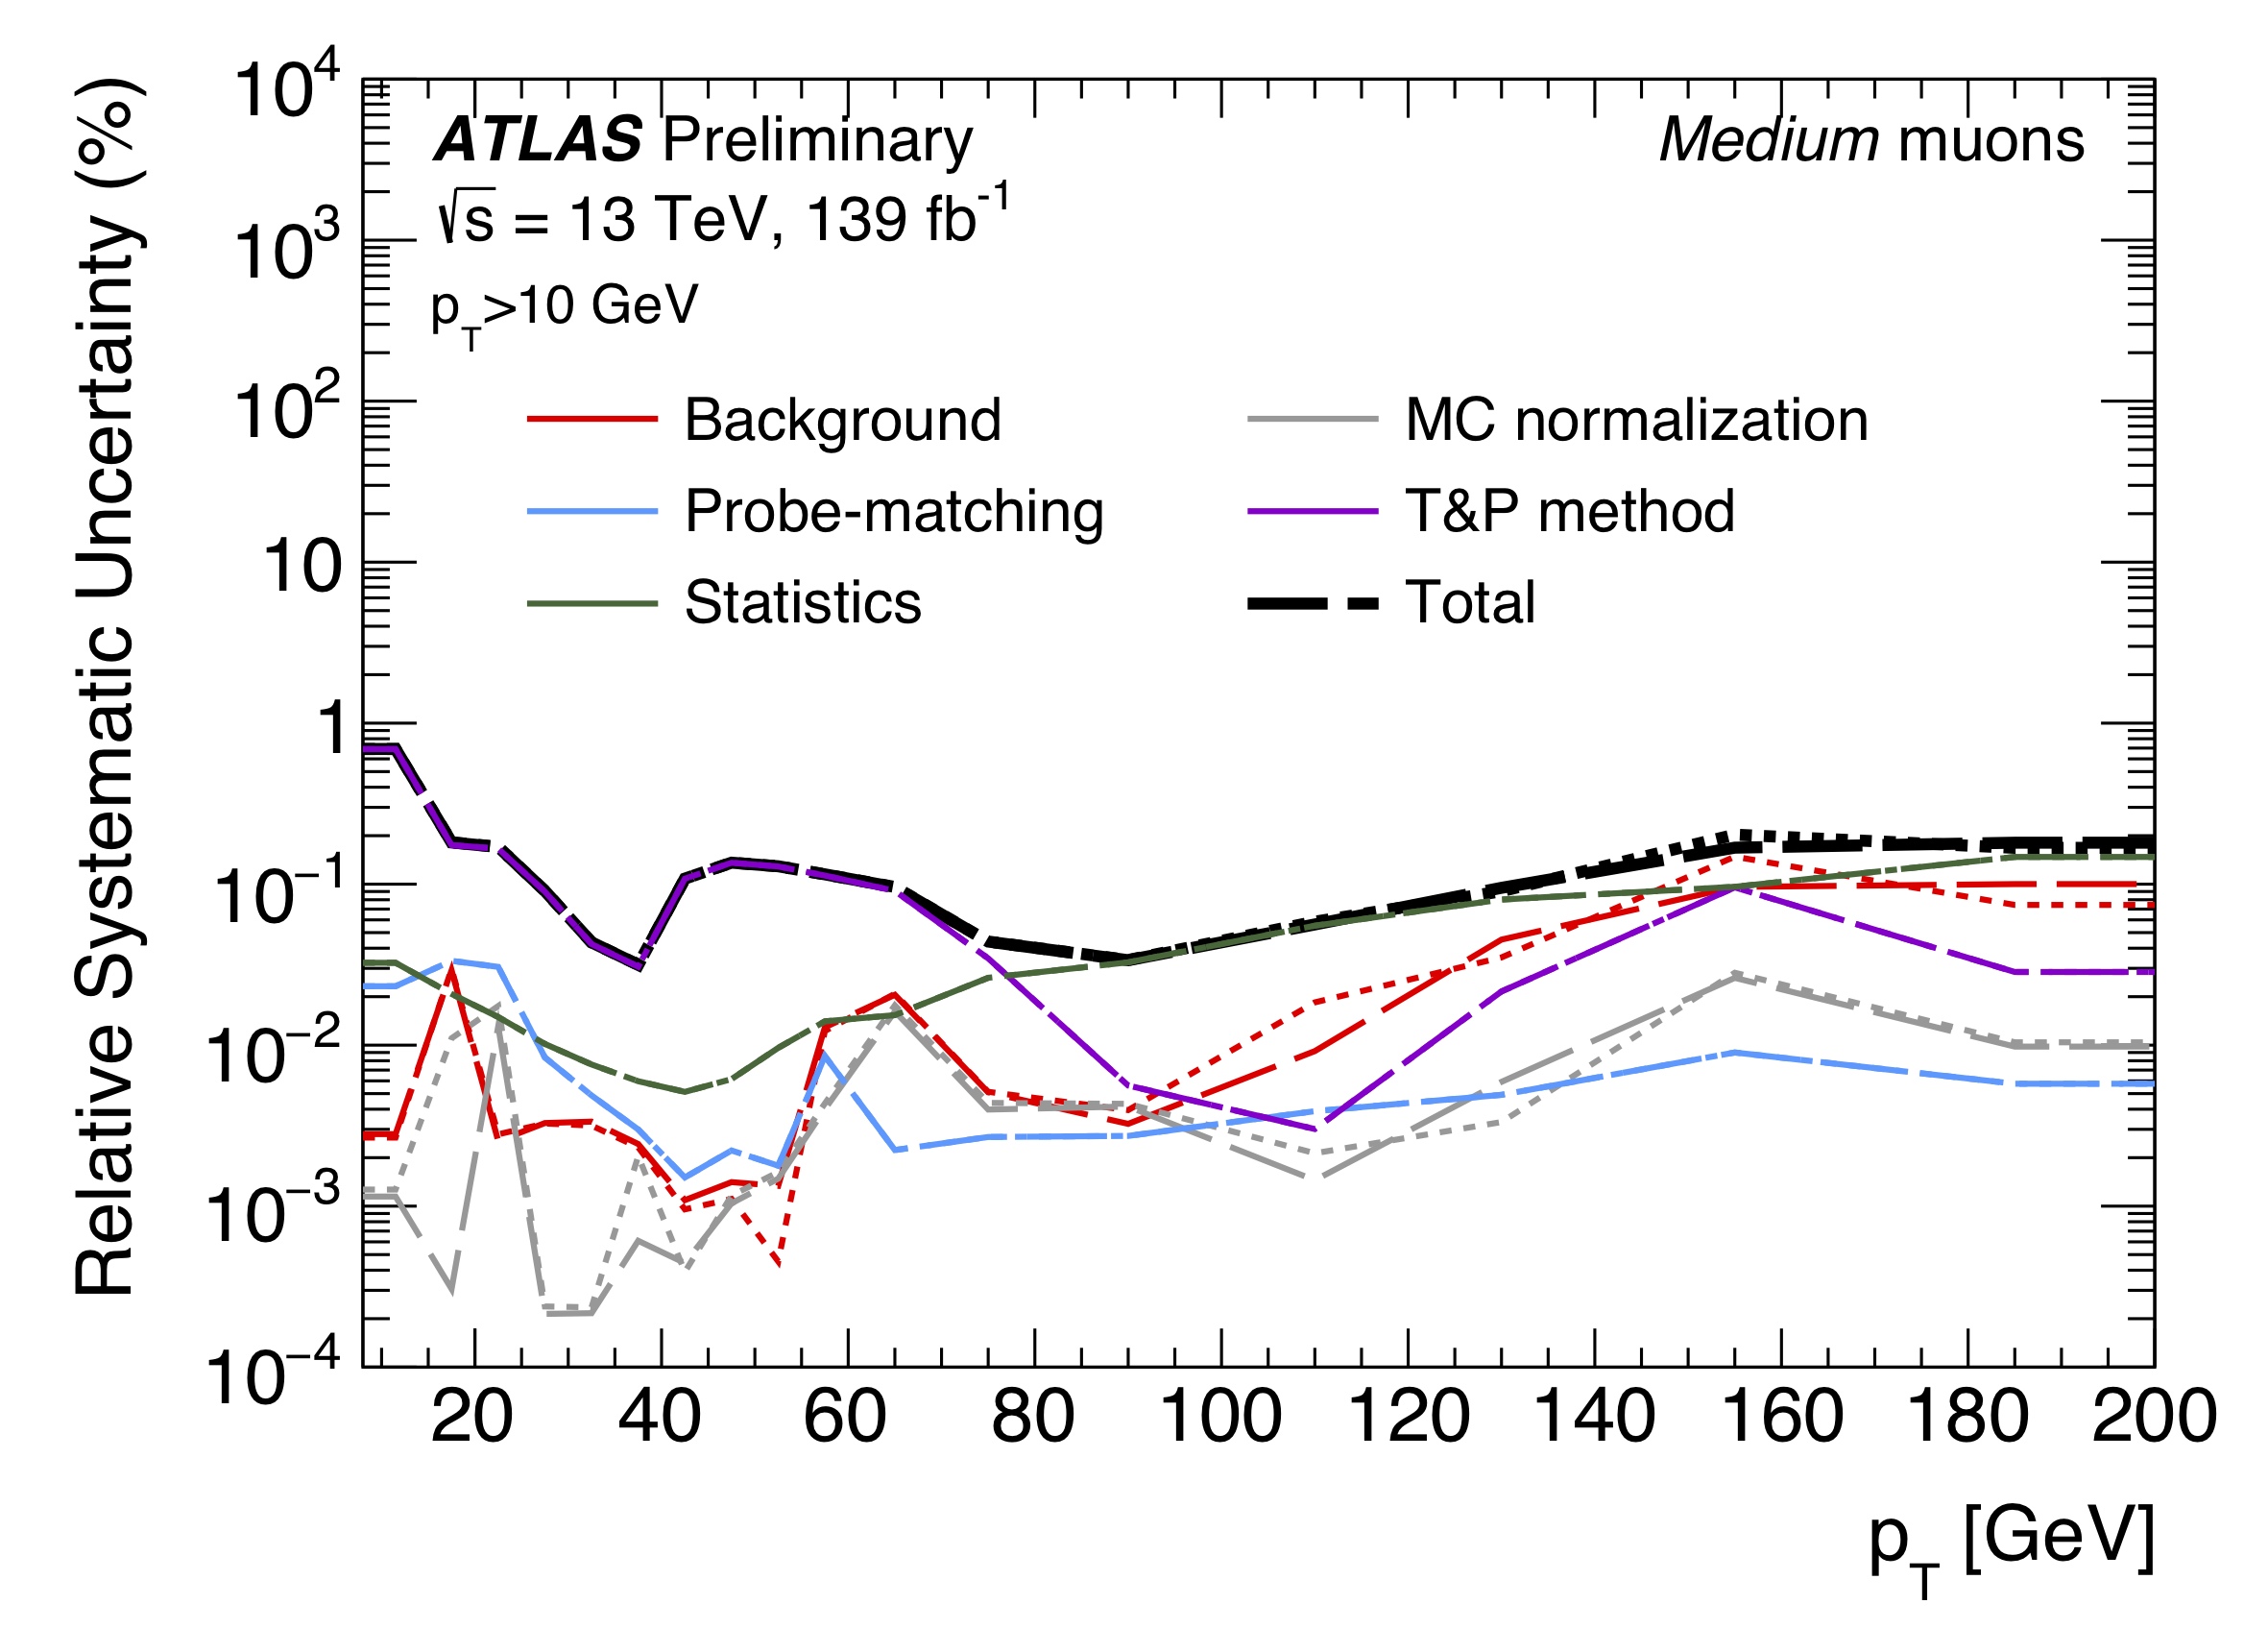
\includegraphics[width=\hsize]{figures/Analysis/muon_syst.png}
  \caption{{This figure shows the breakdown of the muon reconstruction efficiency scale factor measured in $Z \rightarrow \mu \mu$ as a function of $p_{T}$ \cite{muon_calib}. }}. 
  \label{fig:muon_syst}
\end{figure} 
\FloatBarrier

\section{Jets}
Three types of jets are used in this analysis: variable radius, small-R and large-R jets. Variable radius jets are used to reconstruct $Z$ bosons decaying to two $b$-jets in the jet catchment area of large-R jet in the Merged regime. Small-R jets are used to to reconstruct the hadronically decaying $W/Z$ candidates in the resolved analysis and the forward jets from resonances produced through vector boson fusion. Large-R jets are used to reconstruct the hadronically decaying boson in the merged regime.

For these jet collections, the jet energy is calibrated sequentially as shown in Figure \ref{fig:jetcalib}. After the jet direction is corrected to point to the PV, the energy of the jet is corrected. First, the jet energy is corrected to account for pileup contributions based on the $p_{T}$ and area of the jet (these corrections are extracted from a $pp \rightarrow jj$ sample). Following this, another pileup correction is applied that scales with $\mu$ and $N_{PV}$. 

MC-based corrections are then applied that are meant to transform the jet energy and $\eta$ back to particle level as detailed in \cite{jet_energy_calib}. Therefore, these corrections account for the non-compensating nature of the ATLAS calorimeters and inhomogeneity of the detector. Following this, the Global Sequential Calibration is applied that reduces flavor dependence of jet calibrations and accounts for energy leakage of jets outside the calorimeters. Finally, in-situ corrections are applied that account for differences in jet response between data and simulation ($\gamma /Z+$jet and fake lepton samples are used). These differences can arise from mismodeling the hard scattering process, pile-up, and jet formation. 

To further reject jets no arising from the hadronically decaying boson, jets must pass quality requirements based on the following variables \cite{jet_selection}:

\begin{itemize}
\item[-] $f_{Q}^{LAr}$: fraction of energy of jet's LAr cells with poor signal shape
\item[-] $f_{Q}^{HEC}$: fraction of energy of jet's HEC cells with poor signal shape
\item[-] $E_{neg}$: sum of cells with negative energy
\item[-] $f_{EM}$: fraction of jet's energy deposited in EM calorimeter
\item[-] $f_{HEC}$: fraction of jet's energy deposited in HEC calorimeter
\item[-] $f_{max}$: maximum energy fraction in any single calorimeter layer
\item[-] $f_{ch}$: ratio of the scalar sum of the $p_{T}$ of a jet's charged tracks to the jet's $p_{T}$
\end{itemize}

Jets selected for the resolved analysis must pass one of the following criteria, to maintain maximum jet efficiency:

\begin{itemize}
\item[-] $f_{HEC} > 0.5$ and $|f_{Q}^{HEC}| > 0.5$ and $\left\langle Q \right\rangle $ > 0.8, which minimizes jets formed from sporadic noise bursts in the HCAL endcap.
\item[-] $|E_{neg}| > 60$ GeV, which minimizes jets formed from sporadic noise bursts in the HCAL endcap.
\item[-] $f_{EM} > 0.95$ and $f_{Q}^{LAr} > 0.8$ and $\left\langle Q \right\rangle $ > 0.8 and $|\eta| < 2.8$, which minimizes jets formed from large coherent noise or isolated pathological ECAL cells.
\item[-] $f_{max} > 0.99$ and $|\eta| < 2$, which minimizes jets mistakenly formed due to hardware issues, beam-induced backgrounds, and cosmic muon showers.
\item[-] $f_{EM} < 0.05$ and $f_{ch} < 0.05$ and $|\eta| < 2$,which minimizes jets mistakenly formed due to hardware issues, beam-induced backgrounds, and cosmic muon showers.
\item[-] $f_{EM} < 0.05$ and  $|\eta| > 2$, which minimizes jets mistakenly formed due to hardware issues, beam-induced backgrounds, and cosmic muon showers.
\end{itemize}



\begin{figure}[h!]
  \centering
  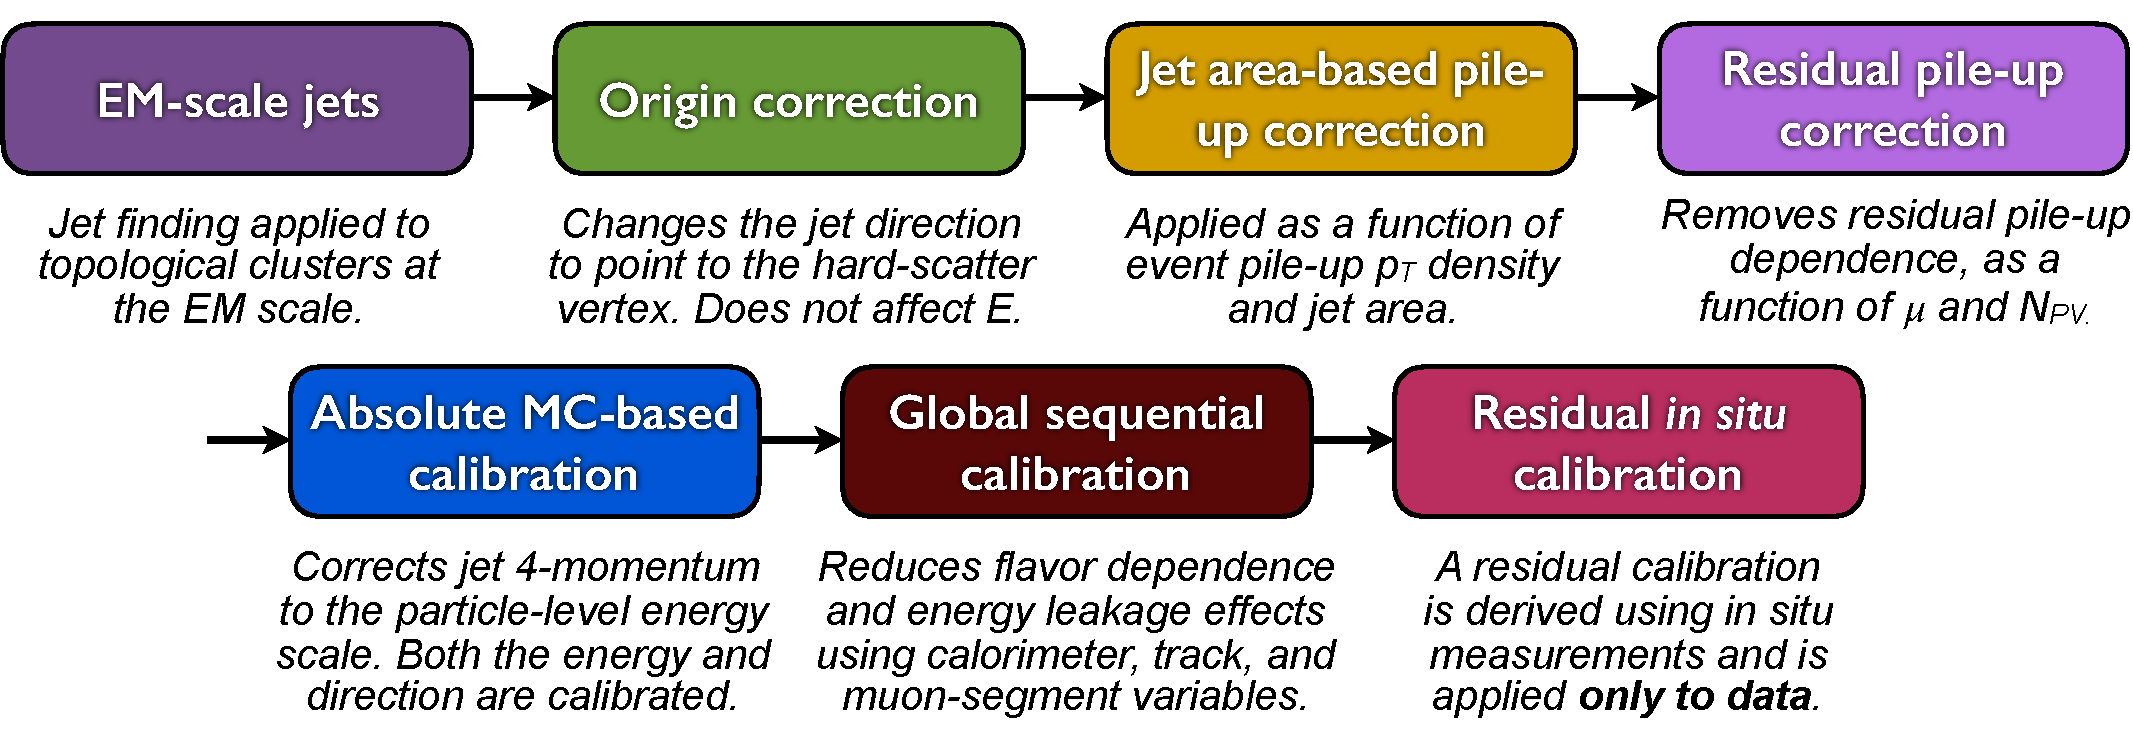
\includegraphics[width=\hsize]{figures/Analysis/jetcalib.pdf}
  \caption{This diagram shows the calibration stages for EM jets \cite{jetcalib} .} 
  \label{fig:jetcalib}
\end{figure} 
\FloatBarrier

\subsection{Small-R jets}
Small-R jets are used to reconstruct the hadronically decaying $W/Z$ candidate when the two resulting jets are well-separated in $\eta$-$\phi$ space. Small-R jets are also used to identify forward jets from resonances produced through vector boson fusion. Small-R jets are constructed from topologically connected clusters of calorimeter cells (topoclusters), seeded from calorimeter cells with energy deposits significantly above the noise threshold.  These cells are then used as inputs to the $anti-k_{t}$ algorithm \cite{antikt} with a radius parameter, R = 0.4, implemented in the FastJet package \cite{fastjet}. 

Jets used in this analysis must have $p_{T} > 30$ GeV and $|\eta| < 2.5$. To further reduce jets not from the hadronically decaying boson the jet-vertex-tagger (JVT) is used \cite{jvt}. The JVT uses two track-based variables, corrJVF and $R_{p_{T}}$ to calculate the likelihood that the jet originated from the PV. The corrJVF variable compares the scalar sum of the $p_{T}$ of tracks associated with the jet and PV to the scalar sum of the $p_{T}$ of tracks associated with the jet. This variable also includes a correction that reduces the dependency of corrJVF with the number of reconstructed vertices in the event. The other discriminant, $R_{p_{T}}$, is given by the ratio of the scalar sum of the $p_{T}$ of tracks associated with the jet and PV to the $p_{T}$ of the jet. Both of these variables peak around zero for pileup jets, as these jets are unlikely to have tracks associated with the PV. JVT cuts are applied to all jets with $p_{T} > 120$ GeV. Central jets ($|\eta| < 2.4$) are required to have a JVT > 0.59 and forward jets ($2.4<|\eta| < 2.5$) are required to have JVT > 0.11. 

\subsection{Large-R jets}
Large-R ($R = 1.0$) jets are used to reconstruct the hadronically decaying $W/Z$ candidate when the resulting jets are not well-separated in $\eta$-$\phi$ space, and overlap forming one large-R jet. Track-Calo Clusters (TCCs) are used to reconstruct these jets \cite{tcc}. These jets are constructed using a pseudo particle flow method using ID tracks matched to calorimeter clusters \cite{particleflow}. To remove contamination in the jet from pileup and the underlying event, jets are trimmed using a re-clustering algorithm. This algorithm removes subjets with $p_{T}^{subjet} < 0.1p_{T}^{jet}$. 

The angular resolution of the calorimeter degrades sharply with jet $p_{T}$, but the jet energy resolution improves. The tracker has excellent angular resolution which improves with $p_{T}$. Therefore, by matching tracks to jets, TCCs have more precise energy and angular resolution than jets constructed from calorimeter information only. These jets are required to have $p_{T}>200$ GeV, $|\eta| < 2.0$ and $m_{J} > 50$ GeV. 

TCC jets are trimmed as detailed in \cite{jet_trimming}, which suppresses pileup and soft radiation in the jet, the jet mass is calculated as the four-vector sum of the jet's constituents (assuming massless constituents). The jet mass peaks around the $W/Z$ boson mass for $W/Z \rightarrow qq$ jets, and more broadly for single-quark and single-gluon induced jets. 

These jets are then tagged as $W$ jet if it passes optimized jet mass and substructure ($D_{2}$) cuts for $W$ bosons, and a $Z$ jet if it passes the cuts for the $Z$ boson. The jet substructure variable $D_{2}$ is given by the ratio of energy correlation functions. These functions are derived from the energies and pair-wise angles of a jet's constituents (\cite{jet_observables}, \cite{boosted_boson}):

\begin{equation}
D_{2}^{\beta=1} = E_{CF3}\left(\frac{E_{CF1}}{E_{CF2}}\right)^{3}
\end{equation}

where the energy correlation functions are defined as:
\begin{equation}
E_{CF1}=\sum_{i}p_{T,i}
\end{equation}
\begin{equation}
E_{CF2}=\sum_{ij}p_{T,i}p_{T,j}\Delta R_{ij}
\end{equation}
\begin{equation}
E_{CF3}=\sum_{ijk}p_{T,i}p_{T,j}p_{T,k}\Delta R_{ij}\Delta R_{jk}\Delta R_{ki}
\end{equation}

A two-dimensional optimization of the jet mass and $D_{2}$ thresholds was performed to provide maximum sensitivity for this analysis. This optimization was done by maximizing the signal sensitivity (using  HVT $W'$ and $G_{KK}$ samples) against the single quark and gluon jet backgrounds in jet $p_{T}$ bins.  Figure \ref{fig:wztag_eff} shows the optimized thresholds on $D_{2}$ and jet mass as a function of $p_{T}$. Figure \ref{fig:boson_tagger_optimization} shows the efficiency of the optimized $W/Z$ taggers as a function of jet $p_{T}$. 


\begin{figure}[h]
%\subfloat[][\label{fig:D2_W}]{
    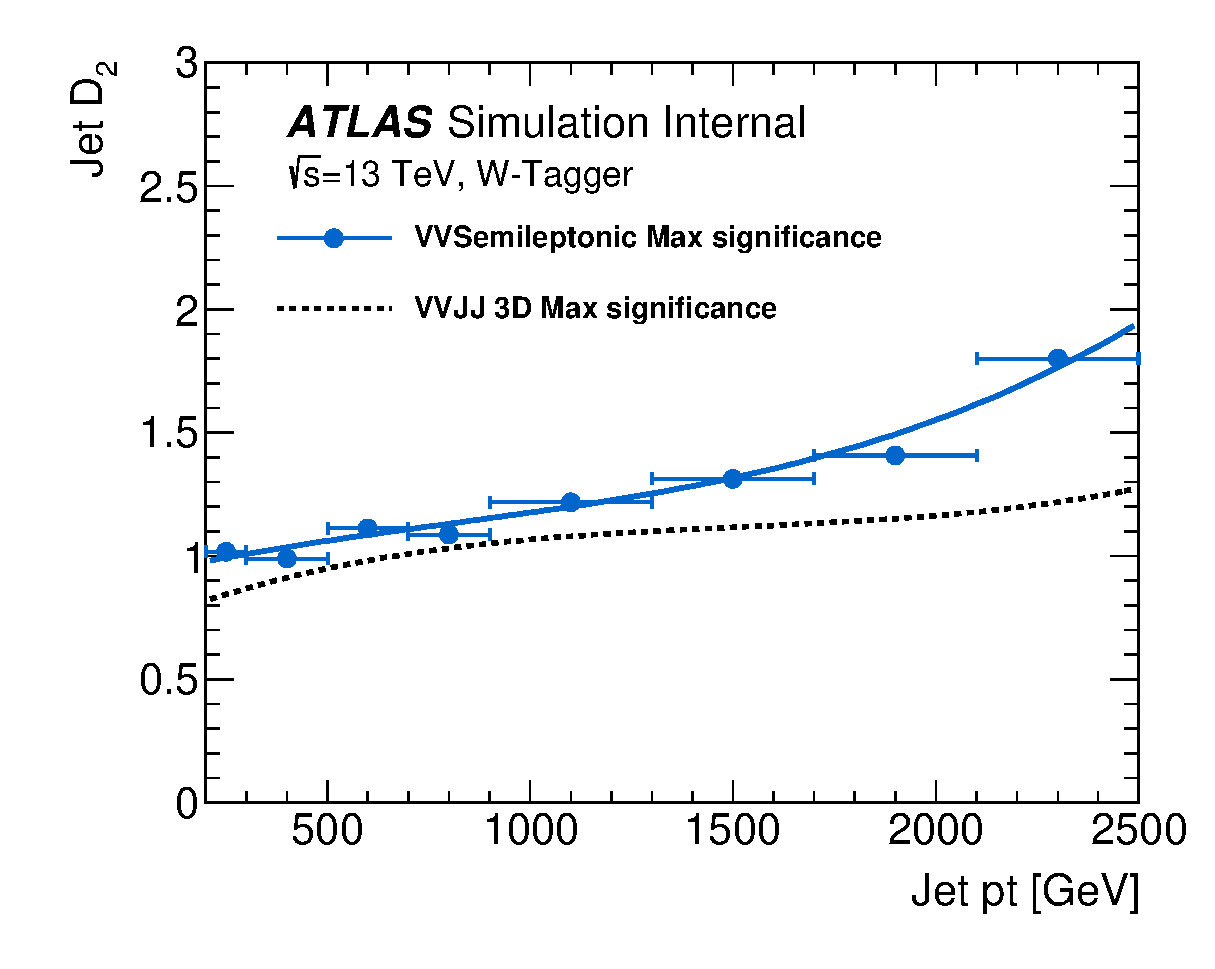
\includegraphics[width=0.48\hsize]{figures/Analysis/D2_W_Fit.eps}
%}
%\subfloat[][\label{fig:Mass_W}]{
    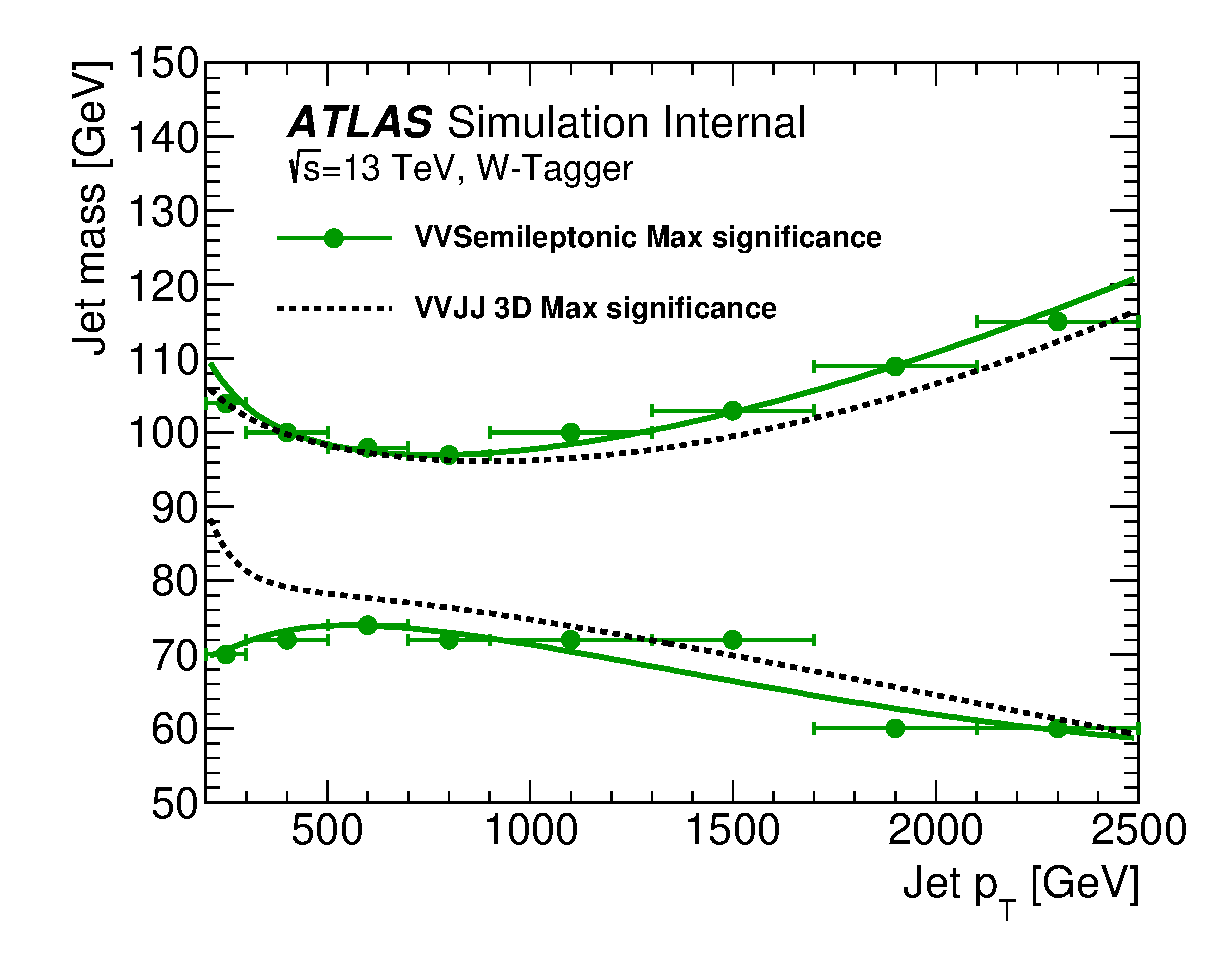
\includegraphics[width=0.48\hsize]{figures/Analysis/Mass_W_Fit.eps}
%}

%\subfloat[][\label{fig:D2_Z}]{
    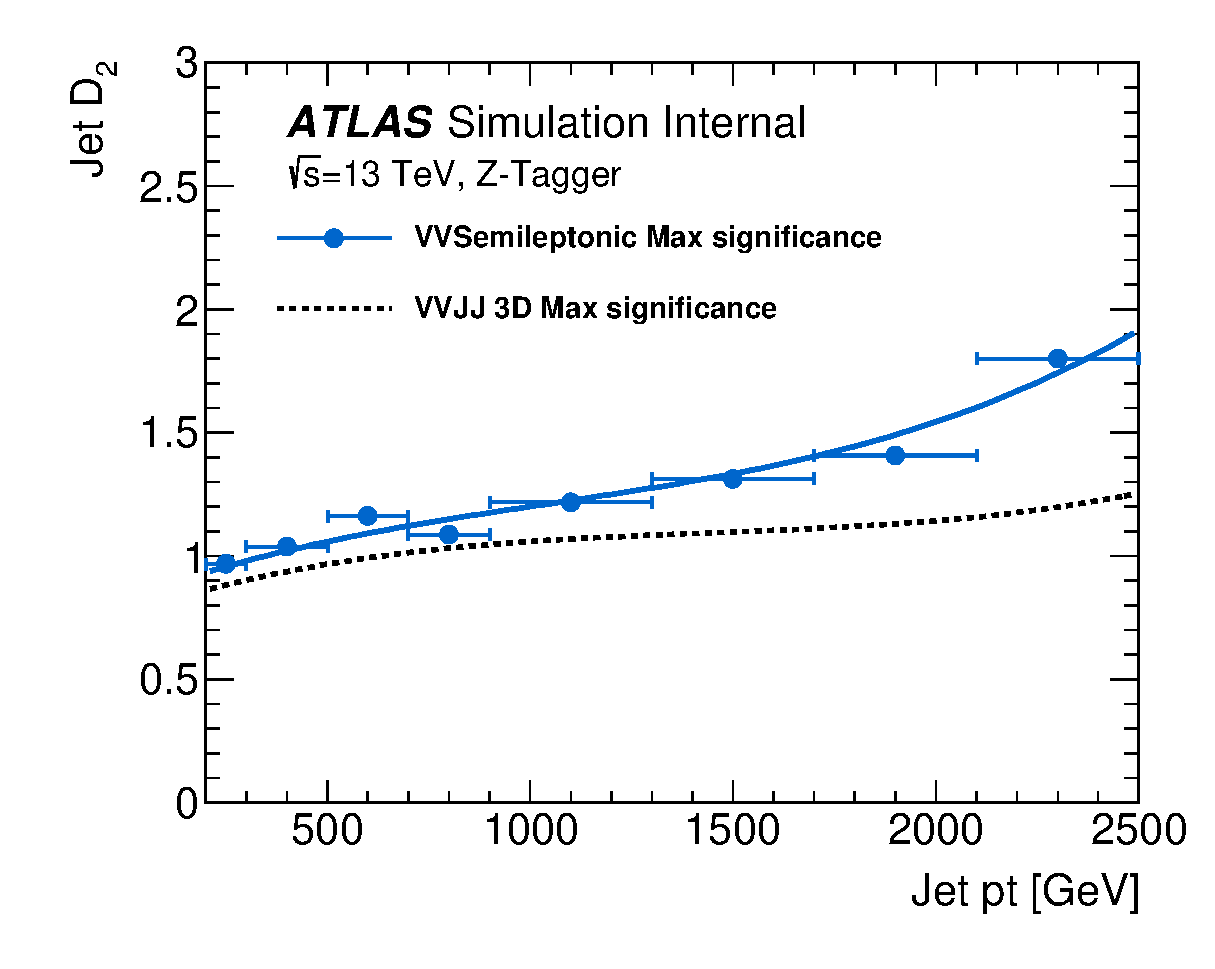
\includegraphics[width=0.48\hsize]{figures/Analysis/D2_Z_Fit.eps}
%}
%\subfloat[][\label{fig:Mass_Z}]{
    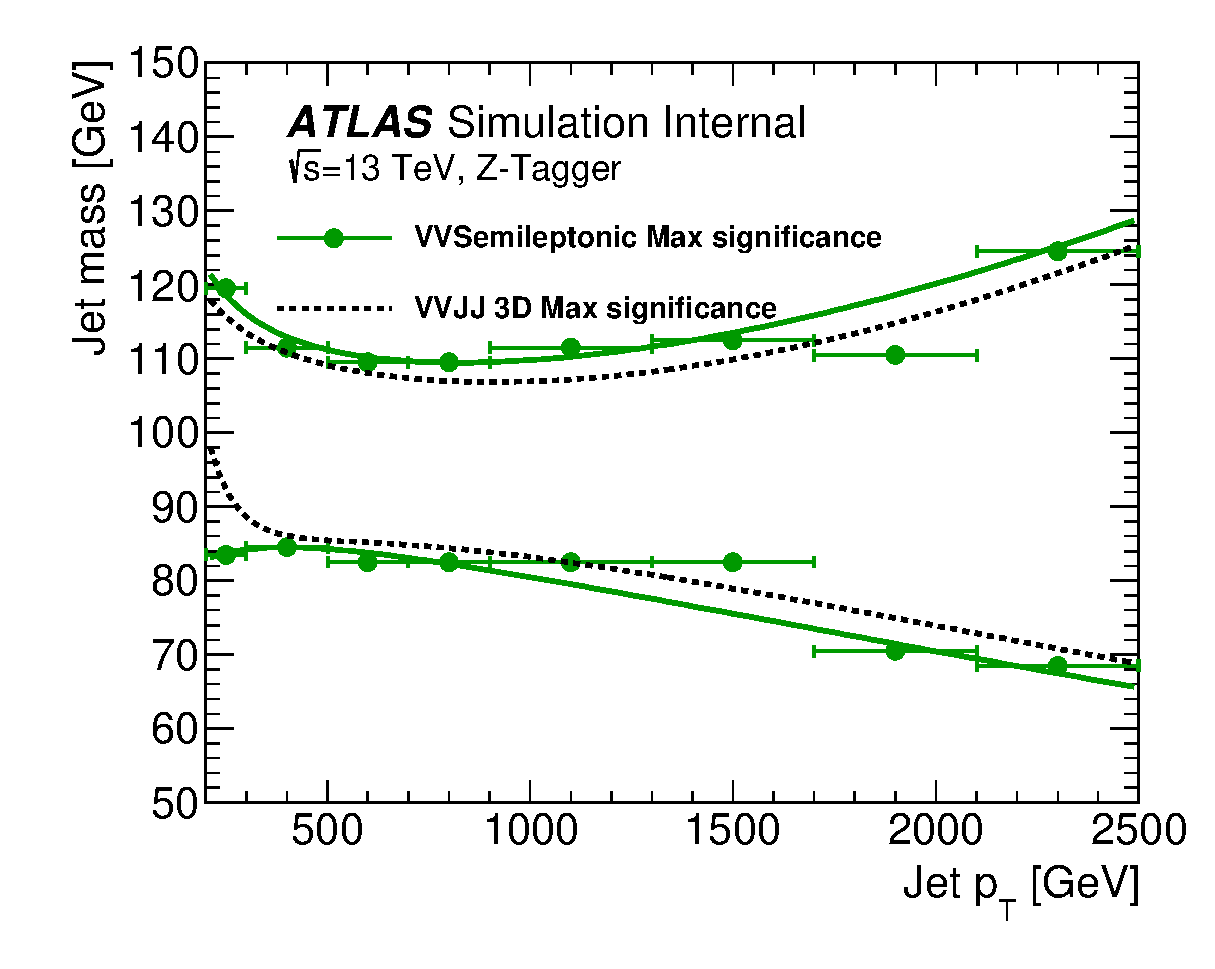
\includegraphics[width=0.48\hsize]{figures/Analysis/Mass_Z_Fit.eps}
%}
\caption{The upper cut on $D_2$ (a) and jet mass window cut i.e. the upper and lower boundary of the mass (b) of the $W$-tagger as a function of jet $p_{T}$. Corresponding values for $Z$-tagger are shown in (c) and (d). The optimal cut values for maximum significance are shown as solid markers and the fitted function as solid lines. Working points from $VV\to JJ$ \cite{VH} is also shown as dashed lines as a reference.}
\label{fig:wztag_eff}
\end{figure}
\FloatBarrier

\begin{figure}[h!]
  \centering
  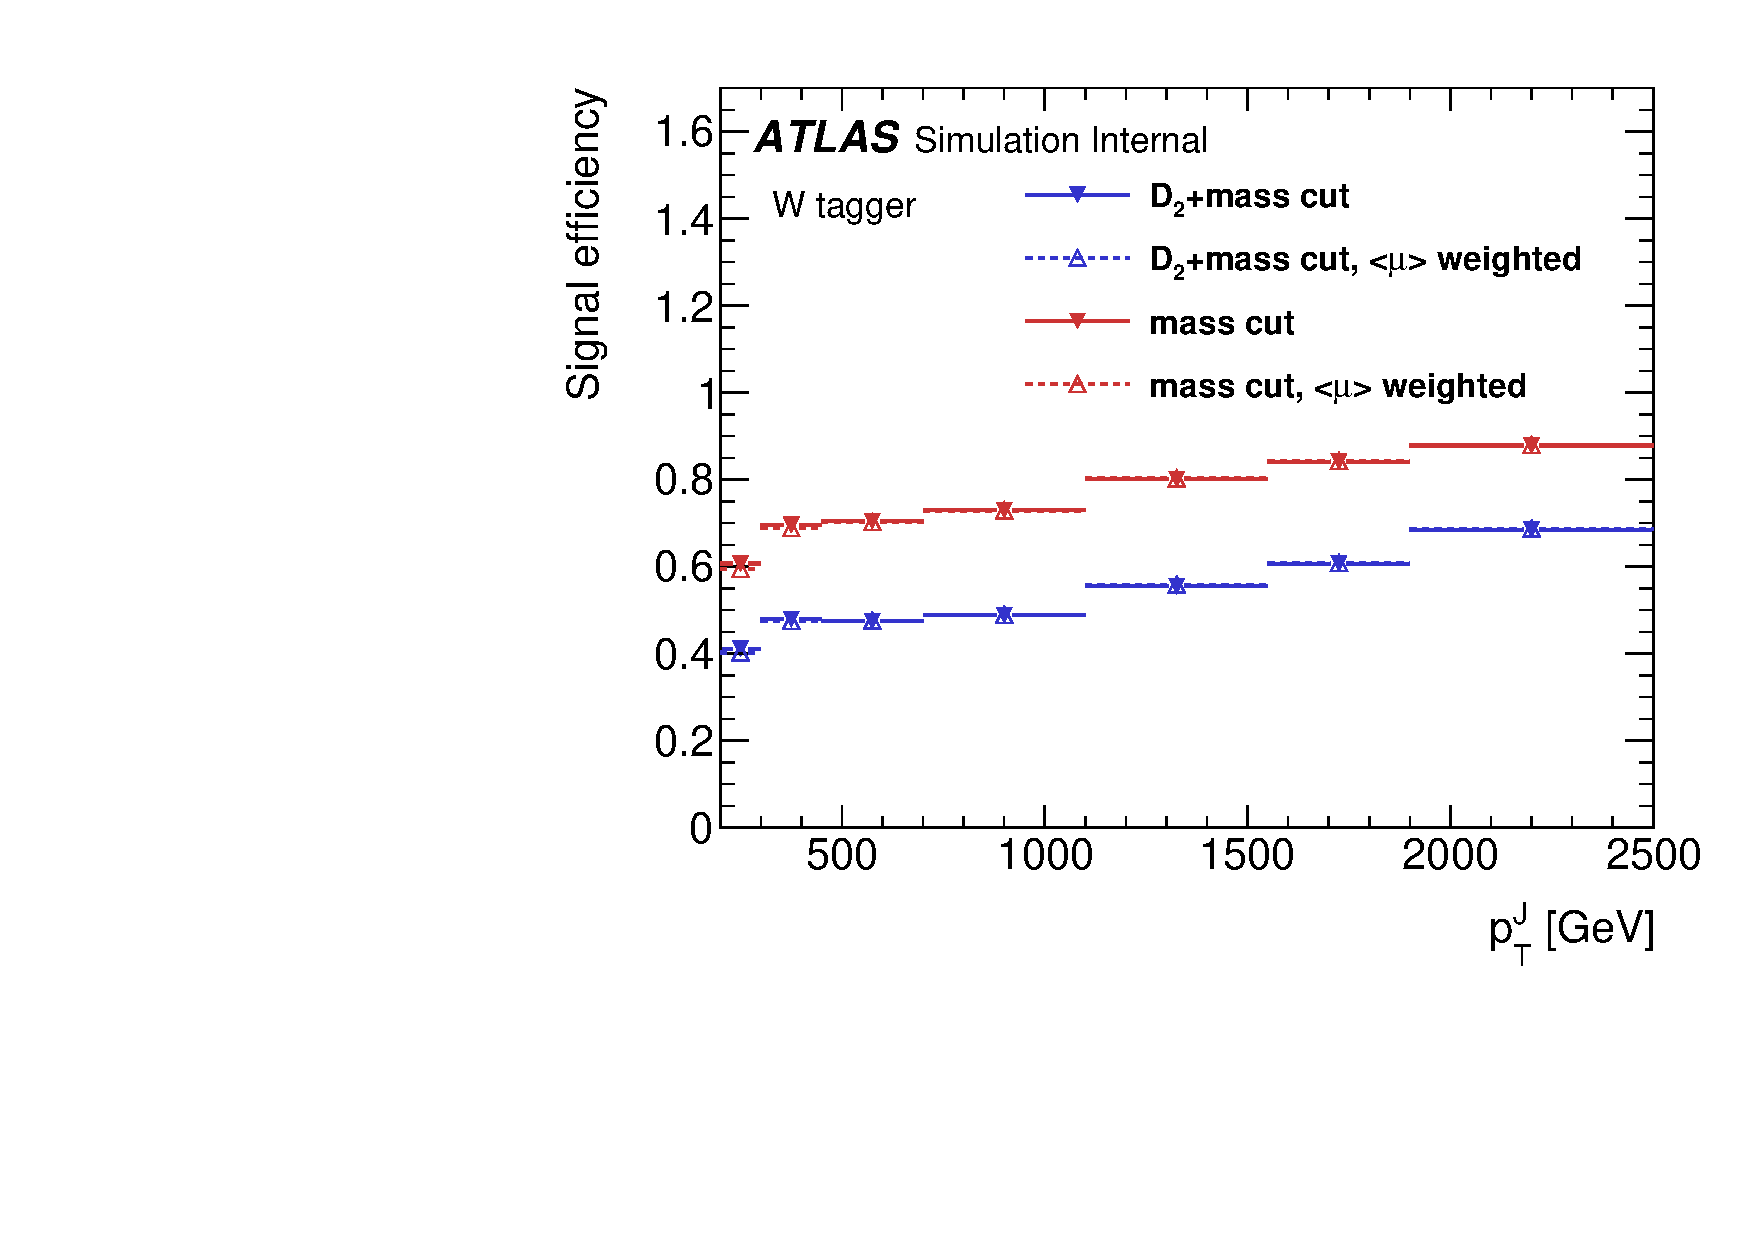
\includegraphics[width=0.48\hsize]{figures/Analysis/sigeffW.pdf}
  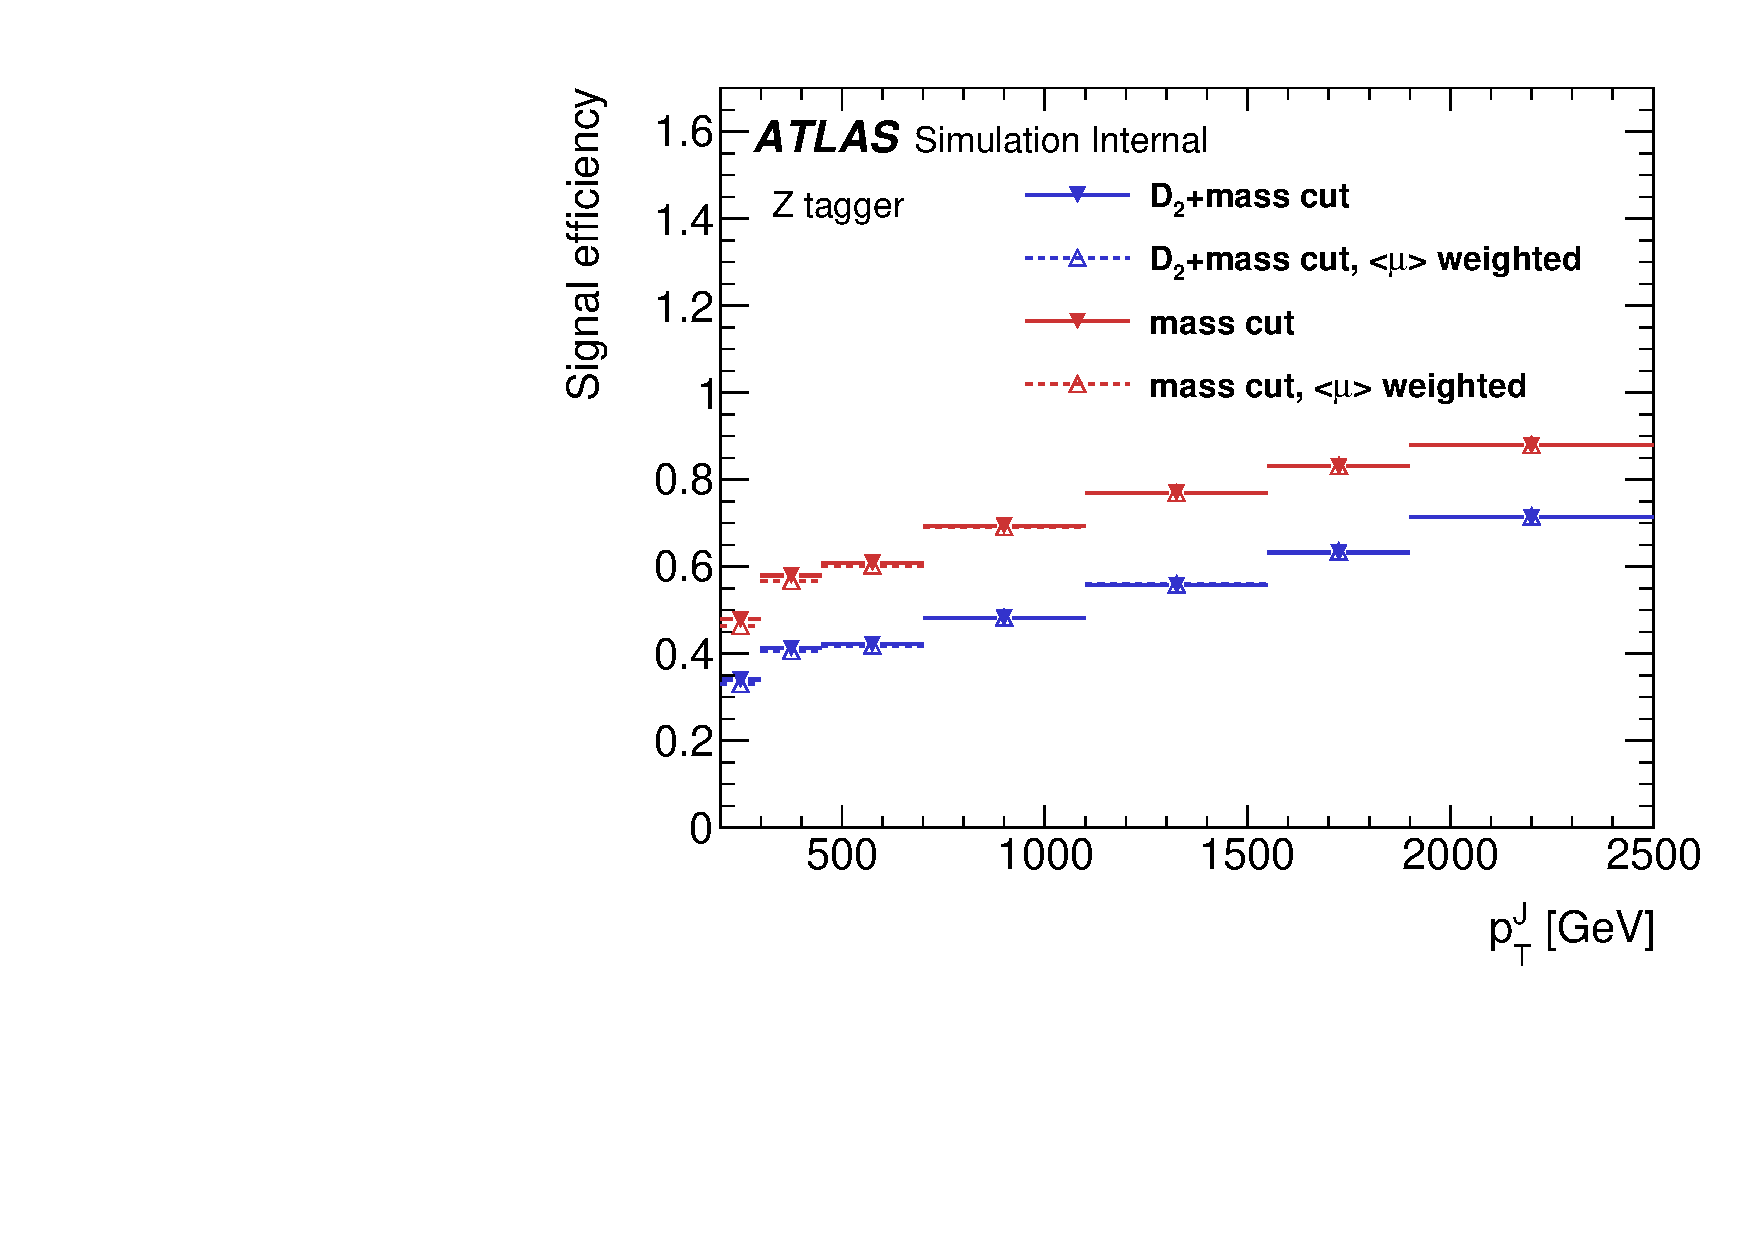
\includegraphics[width=0.48\hsize]{figures/Analysis/sigeffZ.pdf}
  \caption{The left (right) plot shows the efficiency for the $W(Z)$ tagger mass and $D_{2}$ cuts as a function of large-R jet $p_{T}$.} 
  \label{fig:boson_tagger_optimization}
\end{figure} 
\FloatBarrier

\subsection{Variable Radius jets}
To more accept more boosted $Z$ bosons decaying to $b\bar{b}$ that would normally be rejected due to topological cuts discussed \ref{Signal Region Definitions} variable radius (VR) track jets are used to identify $b$-jets (discussed in \ref{Jet Flavor Tagging}) within the catchment area of large-R jets \cite{vrjets}. VR jets are constructed from ID tracks using the anti-$k_{t}$ algorithm with a radius parameter that depends on the $p_{T}$ of the track, shown in Equation \ref{vreq}.
\begin{equation}
R_{eff}(p_{T, i}) = \frac{\rho}{p_{T,i}}
\label{vreq}
\end{equation}
For this search $\rho=30$ GeV and an lower and upper limit on cone size are set to 0.02 and 0.4, respectively, to prevent unphysical asymptotic behavior of $\rho$. Collinear VR jets are possible, so track jets that are not separated by the the smaller jet's cone size are not used. Additionally, VR jets are required to have $p_{T} > $ 10 GeV and $|\eta| < 2.5$. 

\subsection{Jet Flavor Tagging}
\label{Jet Flavor Tagging}
To further classify events, the small-R and VR jets originating from a b-quark are classified using a multivariate $b$-tagging algorithm (BDT), MV2c10 \cite{atlas_btag}. This algorithm uses the impact parameters of the jet's ID tracks, secondary vertices (if they exist), and reconstructed flight paths of $b$ and $c$ hadrons in the jet to determine if the jet was induced by a $b$-quark. For this analysis the 85\% efficient working point of this algorithm is used giving $c$, $\tau$, and light-flavor jet rejection of 3, 8, and 34 respectively in simulated $t\bar{t}$ samples.

\section{MET/Neutrinos}
As neutrinos are uncharged and colorless they do not leave tracks or jets in the detector. For this reason, neutrinos are reconstructed as the missing energy in the event, $E_{T}^{miss}$. Mathematically, $E_{T}^{miss}$ is the negative vector sum of $p_{T}$ all the physics objects and an extra "soft" term. The "soft" term accounts for energy deposits not associated with any of the objects in the event. For this analysis the soft term is given by the sum $p_{T}$ of all ID tracks not associated with objects in the event. The selected tracks must be matched to the primary vertex, which decreases pile-up contamination \cite{met_preformance}. 

\section{Overlap Removal}
Reconstructed jets and leptons in this analysis can arise from the same energy deposits. For instance, a cluster of energy from an electron can also be a valid calorimeter seed for a jet. To mitigate this confusion of multiple objects originating from a single jet or lepton overlapping objects are removed via a procedure referred to a overlap removal. In this procedure the separation of the two objects, $\Delta (R) $, determines which object is removed from the event. 

The overlap selections used in this analysis are:

\begin{itemize}
\item[-] when an electron shares a track with another electron with the lower $p_{T}$ electron is rejected, as it is more likely to be a fake electron
\item[-] when a muon and electron share a track the muon is rejected if it is a calo-muon, otherwise the electron is rejected
\item[-] when $\Delta R < 0.2$ for an electron and jet, the jet is rejected to maximize signal acceptance
\item[-] when $\Delta R > 0.2$ for an electron and jet, the electron is rejected as likely originated from decays within the jet
\item[-] when $\Delta R <$min$(0.4, 0.04+10$GeV/$p_{T}^{\mu})$ the muon is rejected, again maximizing signal acceptance, otherwise the jet is rejected
\item[-] when $\Delta R < 1.0$ for the a large-R jet and electron, the jet is rejected

\end{itemize}

\section{Reconstructed Resonance Mass ($m_{WV}$)}
\label{mwv}
The $WV$ system mass, $m_{WV}$ is reconstructed from the lepton, neutrino, and hadronically-decaying boson candidate. The momentum of the neutrino along the $z$-direction is obtained by constraining the $W$ boson mass of the lepton neutrino system to be  80.3 GeV$/c^{2}$. For complex solutions to this constraint, $p_{Z}$ is taken as the real component of the solution. For real solutions, the one with the smaller absolute value is used. For the resolved analysis, $m_{WV}$ is reconstructed by constraining the $W(Z)$ dijet system in the SRs and TCRs (not the WCRs), which improves the $m_{WV}$ resolution:
\begin{equation}
p^{corr}_{T,jj} = p_{T,jj} \times \frac{m_{W/Z}}{m_{jj}}
\end{equation}
\begin{equation}
m^{corr}_{jj}=m_{W/Z}
\end{equation}
where $m_{jj}$ and $m_{W/Z}$ are the reconstructed invariant mass of the hadronically-decaying W/Z boson and the PDG values of the $W/Z$ boson masses, respectively. The reconstructed resonance mass is the final discriminating variable in this analysis. The distribution of this variable in the CR and SRs are used in the final likelihood fit to search for evidence of an excess of events due to BSM resonances. The distribution of $m_{WV}$ are shown in Figures \ref{fig:hvtww_cr_postfit}-\ref{fig:hvtwzvbf_tag_sr_postfit}. 
\chapter{Event Selection and Categorization}
To search for these new resonances, the simulated background and signal samples are analyzed to determine a series of optimized cuts are used create signal regions (SR) to identify the leptonic and hadronic decay products of the resonance. In these regions, the resonance mass is calculated as the combined system mass of the leptonic and hadronic systems as described in \ref{mwv}. The expected resonance mass distribution from the backgrounds and signal samples are compared to data to search for the existence of these BSM signals (also known as a "bump hunt"). Control regions enriched in the dominant backgrounds, $t\bar{t}$ and $W$+jets (TCR and WCR, respectively) are constructed to be orthogonal to SRs and used to determine the normalization of the $t\bar{t}$ and $W$+jets backgrounds in SRs.

Events are classified as produced via non-VBF or VBF modes using a Recurisve Neural Network described in \ref{rnn}. VBF $W'$ and $Z'$ and ggF $W'$ and $Z'$ resonances studied have unique SR and CR selections to maximize analysis sensitivity. RS Graviton signals are probed using the same selections as the ggF $Z'$ signal. Additionally, more massive resonances are more likely to have boosted $W/Z$ bosons. As the boost of the hadronically decaying boson increases the separation of its hadronic decay products decreases. When the hadronically decaying boson has sufficient boost, the two quarks will overlap and not be identified separately. For this reason, a set of "resolved" selections are used when the hadronic decay products are reconstructed separately, and "merged" selections when the decay products overlap and identified as a single object in the event. A $W/Z$ tagger identifies merged jets as originating from a $W/Z$ bosons based on jet substructure and mass cuts. However, the more boosted the jet is the less likely it is to pass the jet substructure cut, due to track merging. Consequently, the merged selection uses a high purity region (HP), which requires that the jet pass both cuts, and low purity (LP) region where the jet can fail the jet substructure cut. These selections are summarized in \ref{Signal Region Definitions}.

The aforementioned SR definitions veto events with $b$-jets to minimize $t\bar{t}$ contamination. However, $b$-jets are anticipated from $W'$ resonances from the hadronically decaying $Z$ boson. To increase the signal acceptance of these resonances, a $Z\rightarrow bb$ tagger is used to construct additional SR and CRs called the "tagged" regions (and "untagged" if the event fails the $Z\rightarrow bb$ tagger). 

\section{Pre-selection}
Before applying topological cuts, preselection cuts are applied which include trigger and event requirements to reduce background contamination and the dataset size. Events must contain exactly one tight lepton (no additional loose leptons),  the $p_{T}^{\ell \nu} > 75$ GeV, and there must be at least two small-R jets or one large-R jet, so the event is able to pass the resolved or merged selections.
\section{Trigger}
The data were collected using the lowest unprescaled single-lepton or $E_{T}^{miss}$ triggers, as summarized in Table \ref{tbl:triggers}. Since the muon term is not considered in the trigger $E_{T}^{miss}$ calculation, the $E_{T}^{miss}$ trigger is fully efficient to events with high-$p_{T}$ muons. For this reason, the $E_{T}^{miss}$  trigger is used for events where $p_{T}^{\mu} > 150$ GeV, to compensate for the poor efficiency of the single muon trigger above $p_{T}^{\mu}>150$GeV. 


\begin{landscape}
\begin{table}[p]
  \caption{The list of triggers used in the analysis.} \label{tbl:triggers}
\begin{center} 
\small
\begin{tabular}{|l|c|c|c|}
\hline
Data-taking period & $e\nu qq$ channel & $\mu\nu qq$ ($p_{T}(\mu\nu)<150$ GeV) channel & $\mu\nu qq$ ($p_{T}(\mu\nu) > 150$ GeV) channel  \\
\hline
\hline
\multirow{3}{*}{\centering {2015}} & HLT\_e24\_lhmedium\_L1EM20 OR & HLT\_mu20\_iloose\_L1MU15 OR & \multirow{3}{*}{ HLT\_xe70 } \\
 & HLT\_e60\_lhmedium OR & HLT\_mu50 & \\
 & HLT\_e120\_lhloose & & \\
\hline
\multirow{2}{*}{\centering {2016a (run $< 302919$)}} & HLT\_e26\_lhtight\_nod0\_ivarloose OR & HLT\_mu26\_ivarmedium OR  & \multirow{3}{*}{ HLT\_xe90\_mht\_L1XE50 } \\
 & HLT\_e60\_lhmedium\_nod0 OR & HLT\_mu50 &  \\ 
\multirow{2}{*}{($L<1.0\times10^{34}\,{\textrm cm}^{-2}\,{\textrm s}^{-1}$)} & HLT\_e140\_lhloose\_nod0 & & \\
 & HLT\_e300\_etcut & & \\
\hline
{\centering {2016b (run $\geq 302919$)}} & \multirow{2}{*}{same as above} & \multirow{2}{*}{same as above}  &  \multirow{2}{*}{HLT\_xe110\_mht\_L1XE50} \\
($L<1.7\times10^{34}\,{\textrm cm}^{-2}\,{\textrm s}^{-1}$) & & &\\
\hline
{\centering {2017}} & same as above & same as above  &  HLT\_xe110\_pufit\_L1XE55 \\
\hline
{\centering {2018}} & same as above & same as above  &  HLT\_xe110\_pufit\_xe70\_L1XE50  \\
\hline
\end{tabular}
\end{center}
\end{table}
\end{landscape}
\section{non-VBF/VBF RNN}
\label{rnn}
To classify events as originating from non-VBF or VBF production a recursive neural network (RNN) is used \cite{rnn}. This approach is more powerful than a cut-based classification as it improves signal efficiency and analysis sensitivity by exploiting correlations between variables that the RNN learns. In particular, a RNN architecture is ideal as it can handle variable numbers of jets in the events.  

The RNN uses the four-momentum of candidate VBF jets to classify events as VBF or non-VBF topologies. Sometimes jets are incorrectly reconstructed, so the number of jets in the event is expected to vary across the input samples. VBF candidate jets are identified by removing jets from the event that are likely from $W/Z \rightarrow qq$. For the resolved regime this means removing the two leading small-R jets from the VBF candidate jet list. For the merged regime this means removing small-R jets separated by less than 1.0 in $\Delta R$ from the large-R jet. VBF candidate jets are also required to be within $|\eta| < 4.5$. From the list of remaining VBF candidate jets, the two highest-$p_{T}$ jets are chosen. 

The architecture of the RNN is shown in Figure \ref{fig:rnn_architecture}. The RNN is composed of Long Short Term Memory Cells (LSTM) that extract meaningful information and retain it. The logic embedded in the LSTM is shown in Figure \ref{fig:lstm_struct}. LSTMs are useful for VBF event classification for events with two jets, where using the kinematic properties of both jets (and their correlations) will lead to more efficient event classification.

In this RNN architecture, the VBF candidates are first passed to a masking layer which checks the number of jets in the event. If there is only one jet, only one vertical LSTM layer is used. The output of masking is then passed to a LSTM, with a tanh activation function. The output of the LSTM is then passed to a second horizontal LSTM layer (and vertical LSTM layer if there are two jets in the event). Finally the output of the last LSTM cell is passed to a dense layer and then to a sigmoid activation layer, leading to an overall RNN score.

The weights and other parameters of the network are learned by training the network with HVT VBF and non-VBF signals and all simulated backgrounds over 200 epochs with an Adam Optimizer \cite{adamopt}. To prevent overfitting during training, dropout is applied to RNN weights and training is truncated if the network parameters are unchanged after ten iterations \cite{rnndropout}. Figure \ref{fig:rnn_roc} shows the ROC curve for the RNN using k-fold cross validation \cite{kfold}. 

 Figure \ref{fig:rnn_score} shows the RNN discriminant for backgrounds, non-VBF signals, and VBF signals. The RNN score is $\sim$ 0 for non-VBF signals and background processes and $\sim$1 for VBF processes. Figure \ref{fig:rnn_limits} shows the limits for various signal processes based on the RNN cut applied. Requiring the RNN score to be $>$ 0.8 was chosen as it provided the best analysis significance for this final state and the $\nu\nu qq$ and $\ell \ell qq$ channels, which this channel will be combined with for future publications.


\begin{figure}[h!]
  \centering
  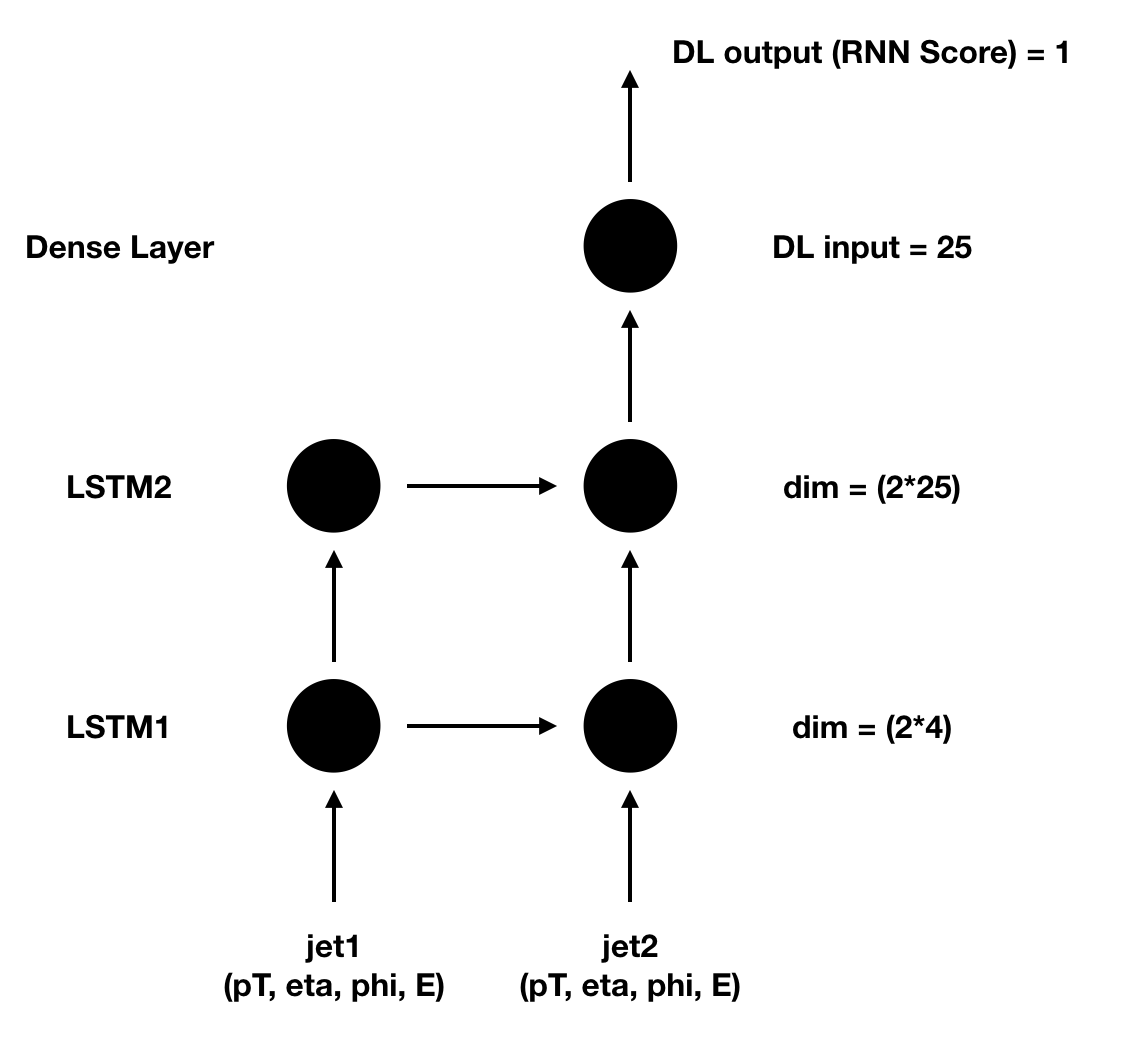
\includegraphics[width=\hsize]{figures/Analysis/rnn_architecture.png}
  \caption{This figure shows the architecture of the RNN used to classify events as non-VBF/VBF. The two VBF candidate jet's variable are passed to a through two layers of LSTMs. The vector output of the final LSTM is combined to give the scalar output of the RNN used to classify the event as non-VBF/VBF. } 
  \label{fig:rnn_architecture}
\end{figure}
\FloatBarrier

\begin{figure}[h!]
  \centering
  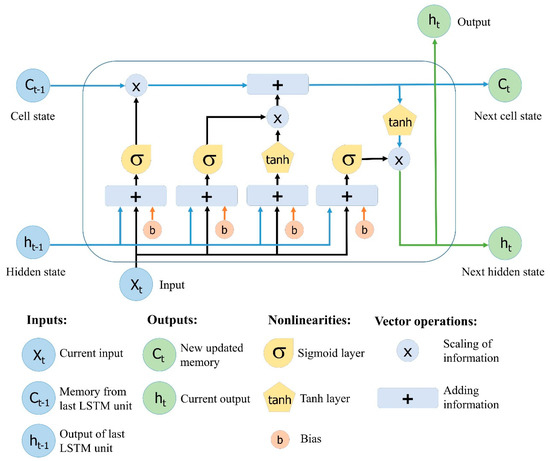
\includegraphics[width=\hsize]{figures/Analysis/LSTM_structure.jpeg}
  \caption{This figure shows the embedded logic in LSTM cells. This image was taken from \cite{lstmstruct}, where a more in depth discussion about LSTMs may be found. }
  \label{fig:lstm_struct}
\end{figure}
\FloatBarrier


\begin{figure}[h!]
  \centering
  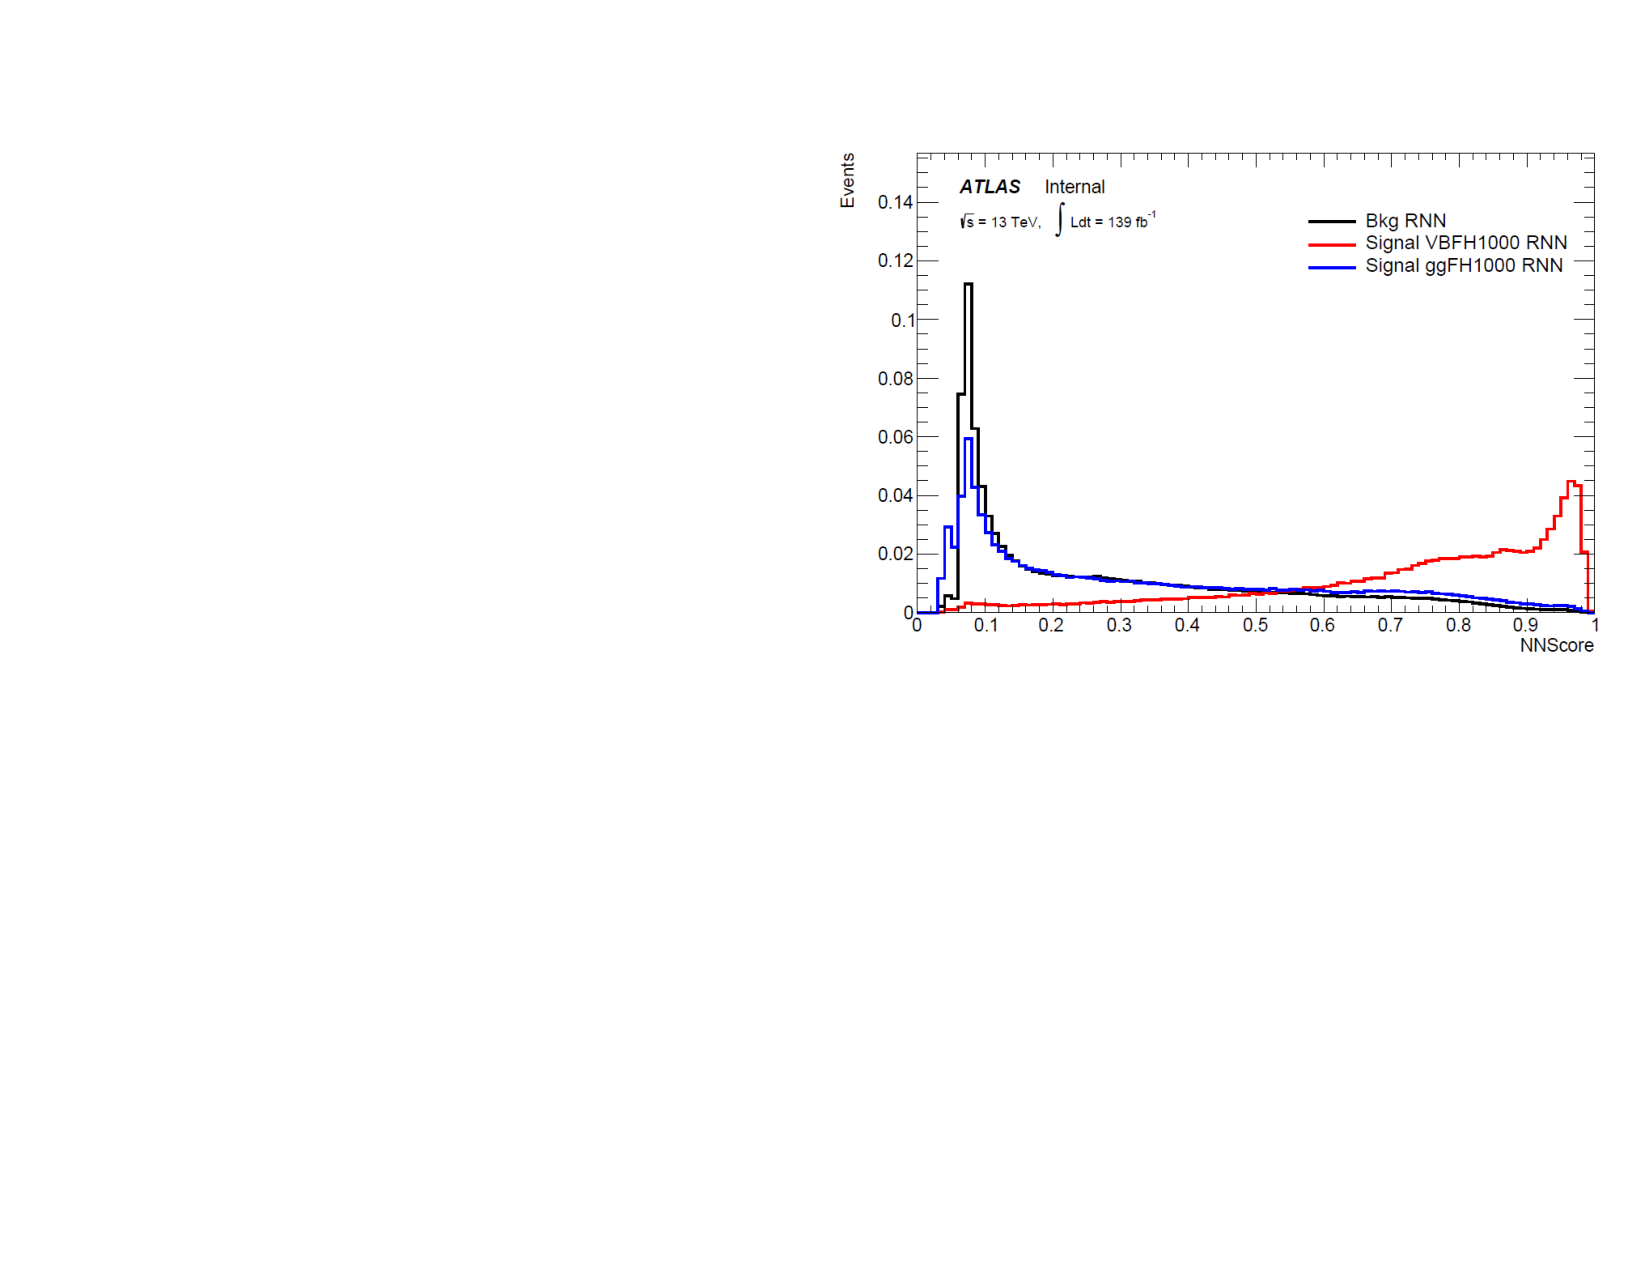
\includegraphics[width=\hsize]{figures/Analysis/rnn.pdf}
  \caption{RNN Score distribution for ggF and VBF signals and backgrounds.} 
  \label{fig:rnn_score}
\end{figure}
\FloatBarrier



\begin{figure}[h!]
  \centering
  \includegraphics[width=\hsize]{figures/Analysis/kFold_ROC.png}
  \caption{ROC curve using k-fold validation for RNN.} 
  \label{fig:rnn_roc}
\end{figure}
\FloatBarrier



\begin{figure}[h!]
  \centering
  \includegraphics[width=\hsize]{figures/Analysis/rnn_limits.pdf}
  \caption{Comparison of ggF Z' limits for different RNN score selections. The bottom panel shows the ratio of the upper limits set for different RNN cuts to the cut-based analysis. In this panel smaller numbers, indicate that the expected upper limit is smaller than the cut-based analysis, which is desired.} 
  \label{fig:rnn_limits}
\end{figure}
\FloatBarrier

\section{Signal Region Definitions}
\label{Signal Region Definitions}
Signal regions are constructed to be dominated by signal and used in the final likelihood fit to look for a bump in the reconstructed resonance mass distribution. Once an event is classified by the RNN, it must pass topological cuts that maximize $S/\sqrt{B}$. To efficiently select events with a $W\rightarrow \ell \nu$ candidate exactly one tight lepton is required and $E_{T}^{miss} > 100(60)$ GeV and $p_{T,\ell\nu} > 200(75)$ GeV in the merged (resolved) analysis to suppress the fake lepton backgrounds. 

The resonances this search probes are expected to be produced approximately at rest with the two resulting bosons produced back-to-back. For this reason, it is required that the minimum value of $(p_{T, \ell \nu}, p_{T,J})/m_{WV} > 0.35(0.25)$ for the non-VBF (VBF) category. 

To reduce $t\bar{t}$ contamination in the merged HVT $Z'$ and $G_{KK}$ analyses, events with at least one $b$-jet with $\Delta R > 1.0$ from the large-R jet are excluded. High purity signal regions require the $D_{2}$ and $W/Z$ mass window cut to be passed, whereas the low purity region only requires the  $W/Z$ mass window cut to be passed. More boosted jets, are more likely to fail the $D_{2}$ cut due to track merging. Therefore, by using high and low purity regions, the signal acceptance is increased. 

The HVT $W'$ resonance search uses tagged and untagged regions to minimize backgrounds and increase signal acceptance. For events to be classified as tagged the large-R jet must contain exactly two $b$-tagged VR jets. Untagged events must have no more than one $b$-tagged jet matched to the large-R jet. These selections are shown in Table \ref{tab:SRdefinitions_1lep_merged}. 

Events failing the merged selection are then re-analyzed in the resolved category. To enhance resolved signals, the event should contain one leptonic and one hadronic boson candidate that are back-to-back in $\phi$ as shown by the selections in Table \ref{tab:SRdefinitions_1lep_resolved}. Again, to suppress the $t\bar{t}$ backgrounds, events are required to have no additional $b$-jets for the HVT $Z'$ and $G_{KK}$ analyses. A summary of the resolved selections is shown in Table \ref{tab:SRdefinitions_1lep_resolved}.

The analysis cutflow in Figure \ref{fig:cutflow} shows how the different categories are prioritized. Events classified as VBF events are classified as merged high purity, low purity or resolved signal region selections sequentially. If the event does not pass any of these selections but passes a VBF control region selection it is classified as a VBF CR event. 

If the event fails all VBF categories, it is then checked if it passes the merged high purity, low purity or resolved signal region selections (NB: for the $WZ$ decay modes all the regions have tagged and untagged categories). If the event fails all of the non-VBF signal region selections, it is then kept for non-VBF control region selections, if it passes those selections. Control region selection are discussed more in \ref{crs}.

Overall, for the Drell-Yan HVT $Z'$ and gluon-gluon fusion $G_{KK}$ signals there are 3 signal regions. For the Drell-Yan HVT $W'$ signal there are 6 signal regions. For VBF HVT $W'$ and $Z'$ signals there are 3 signal regions.

\begin{table}[t]
  \caption{Summary of selection criteria used to define the signal region (SR), $W$+jets control region ($W$ CR) and $t\bar{t}$ control region ($t\bar{t}$ CR) for merged 1-lepton channel.} \label{tab:SRdefinitions_1lep_merged}
\begin{center}
\resizebox{\textwidth}{!}{
\begin{tabular}{|l|l|c|c|c|c|c|c|}
\hline
\multicolumn{2}{|l|}{\multirow{2}{*}{Selection}} & \multicolumn{2}{c|}{SR}  &  \multicolumn{2}{c|}{$W$ CR (WR)}  & \multicolumn{2}{c|}{$t\bar{t}$ CR (TR1)} \\
\cline{3-8}
\multicolumn{2}{|l|}{} & HP & LP &HP & LP & HP & LP \\
\hline
\multirow{4}{*}{$W\rightarrow \ell\nu$} & Num of Tight leptons & \multicolumn{6}{c|}{ 1 } \\
\cline{2-8}
&Num of Loose leptons & \multicolumn{6}{c|}{ 0 }  \\
\cline{2-8}
&\vphantom{\Large B} $E_{T}^{miss}$& \multicolumn{6}{c|}{ $>100$ GeV } \\
\cline{2-8}
&$p_{T}(\ell\nu)$ & \multicolumn{6}{c|}{ $>200$ GeV } \\
\hline
\multirow{4}{*}{$W/Z\rightarrow J$} & Num of large-$R$ jets & \multicolumn{6}{c|}{ $\geq 1$ } \\
\cline{2-8}
& \vphantom{\Large B} $D_2$ cut & pass & fail & pass & fail & pass & fail \\
\cline{2-8}
 & $W/Z$ mass window cut & pass & pass & fail & fail & pass & pass\\
\cline{2-8}
 & Numb. of associated VR track jets $b$-tagged & \multicolumn{6}{c|}{ For $Z\to J$: $\leq 1$ ($= 2$) for untagged (tagged) category } \\
\hline
Topology cut & $\min \left( p_{T,\ell\nu}, p_{T,J} \right)/ m_{WV}$ & \multicolumn{6}{c|}{ $>0.35 (0.25)$ for DY/ggF (VBF) category } \\
\hline
Top-quark veto & Num of $b$-tagged jets outside of large-R jet & \multicolumn{4}{c|}{0} & \multicolumn{2}{c|} {$\geq 1$} \\
\hline
\multicolumn{2}{|c|}{Pass VBF selection} & \multicolumn{6}{c|}{ no (yes) for DY/ggF (VBF) category } \\
\hline
\end{tabular}
}
\end{center}
\end{table}


\begin{table}[t]
  \caption{The list of selection cuts in the resolved analysis for the $WW$ and $WZ$ signal regions (SR), $W$+jets control region (WR) and $ t\bar{t}$ control region (TR).} \label{tab:SRdefinitions_1lep_resolved}
\begin{center} 
\resizebox{\textwidth}{!}{
\begin{tabular}{|l|l|c|c|c|}
\hline
\multicolumn{2}{|l|}{cuts} & SR & $W$ CR (WR) & $t\bar{t}$ CR (TR1) \\
\hline
\multirow{4}{*}{$W\rightarrow \ell\nu$ } & Number of Tight leptons & \multicolumn{3}{c|}{ 1 } \\
\cline{2-5}
&Number of Loose leptons & \multicolumn{3}{c|}{ 0 }  \\
\cline{2-5}
&$E_{T}^{miss}$ & \multicolumn{3}{c|}{ $> 60$ GeV } \\
\cline{2-5}
&$\$p_{T}(\ell\nu)$ & \multicolumn{3}{c|}{ $> 75$ GeV } \\
\hline
\multirow{7}{*}{$W/Z\rightarrow jj$ } & Number of small-R jets & \multicolumn{3}{c|}{ $\geq2$ } \\ %$\geq 2$ & $\geq 2$ & $\geq 2$  \\
\cline{2-5}
& Leading jet $p_{T}$ & \multicolumn{3}{c|}{ $> 60$ GeV}\\
\cline{2-5}
& Subleading jet $p_{T}$ & \multicolumn{3}{c|}{ $> 45$ GeV}\\
\cline{2-5}
 &$Z \rightarrow q\bar{q}$     &   $78 < m_{jj} < 105$ GeV & $50 <m_{jj} < 68$ GeV or & \multirow{2}{*}{$50 < m_{jj} < 150$ GeV} \\
 &$W \rightarrow q\bar{q}$     &   $68 < m_{jj} < 98$ GeV & $105 < m_{jj} < 150$ GeV & \\
\cline{2-5}
 & Num. of $b$-tagged jets &  \multicolumn{3}{c|}{ For $Z\to jj$: $\leq 1$ ($=2$) for untagged (tagged) category } \\
\hline
\multirow{5}{*}{Topology cuts} & $\Delta\phi(j,\ell)$ & \multicolumn{3}{c|}{ $>1.0$}\\
\cline{2-5}
& $\Delta\phi(j,E_{T}^{miss})$ & \multicolumn{3}{c|}{ $>1.0$}\\
\cline{2-5}
& $\Delta\phi(j,j)$ & \multicolumn{3}{c|}{ $<1.5$}\\
\cline{2-5}
& $\Delta\phi(\ell,E_{T}^{miss})$ & \multicolumn{3}{c|}{ $<1.5$}\\
\cline{2-5}
& $\min \left( p_{T,\ell\nu},  p_{T,jj} \right) / m_{WV}$ &\multicolumn{3}{c|}{$>0.35 (0.25)$ for DY/ggF (VBF) category}\\
\hline
Top veto &  Number of additional $b$-tagged jets & \multicolumn{2}{c|}{0} & $\geq 1$ \\
\hline
\multicolumn{2}{|c|}{Pass VBF selection} & \multicolumn{3}{c|}{ no (yes) for DY/ggF (VBF) category } \\
\hline   
\end{tabular}
}
\end{center}
\end{table}


\begin{figure}[h!]
  \centering
  \includegraphics[width=\hsize]{figures/Analysis/cutflow.pdf}  
  \caption{This diagram shows the prioritization scheme used to classify events into the various SRs and CRs. The VBF regions are prioritized over the non-VBF regions and the merged analysis is prioritized over the resolved analysis.} 

  \label{fig:cutflow}
\end{figure} 
\FloatBarrier

\section{Selection Acceptance and Efficiency}
The signal acceptance is the ratio of the number of signal events selected to the number of signal events generated at truth level, which does not account for detector effects. The signal efficiency is the ratio of the number of reconstructed events selected and the number of truth events selected, which accounts for detector effects. The expected number of signal events is given by the product of these two quantities:

\begin{equation}
A \cdot \epsilon = \frac{N^{\mathrm{truth}}_{\mathrm{events\, selected}}}{N^{\mathrm{truth}}_{\mathrm{events\, generated}}} \cdot \frac{N^{\mathrm{reco}}_{\mathrm{events\, selected}}}{N^{\mathrm{truth}}_{\mathrm{events\, selected}}}
\\
= \frac{N^{\mathrm{reco}}_{\mathrm{events\, selected}}}{N^{\mathrm{truth}}_{\mathrm{events\, generated}}}
\end{equation}
The distributions of $A\cdot \epsilon$ as a function of the resonance mass for the different spin models are shown in Figures \ref{fig:accept_hvtww} - \ref{fig:accept_rsg}.

\begin{figure}[h!]
  \centering
\includegraphics[width=0.48\hsize]{figures/Analysis/signal_acceptance/Acc_times_Eff1lepDYHVT.pdf}
    \includegraphics[width=0.48\hsize]{figures/Analysis/signal_acceptance/Acc_times_Eff1lepVBFHVT.pdf}

      \caption{Selection acceptance times efficiency for the $W'\to WZ\to \ell \nu qq$ events from MC simulations as a function of the $W'$ mass for Drell-Yan (left) and VBF production (right), combining the merged HP and LP signal regions of the $WV\to \ell\nu J$ selection and the resolved regions of the $WV\to \ell\nu jj$ selection. Note: the VBF selection acceptance for the DY $W'$ is approximately zero in the left plot.} 
  \label{fig:accept_hvtww}
\end{figure} 
\FloatBarrier


\begin{figure}[h!]
  \centering
\includegraphics[width=0.48\hsize]{figures/Analysis/signal_acceptance/Acc_times_Eff1lepggFRSG.pdf}
    \includegraphics[width=0.48\hsize]{figures/Analysis/signal_acceptance/Acc_times_Eff1lepVBFRSG.pdf}

      \caption{Selection acceptance times efficiency for the $G\to WW\to \ell \nu qq$ events from MC simulations as a function of the $G$ mass for (a) Drell-Yan and (b) VBF production, combining the merged HP and LP signal regions of the $WV\to \ell\nu J$ selection and the resolved regions of the $WV\to \ell\nu jj$ selection. Note: the VBF selection acceptance for the ggF $G_{KK}'$ is approximately zero in the left plot.} 
  \label{fig:accept_rsg}
\end{figure} 
\FloatBarrier
\chapter{Background Estimate}
Backgrounds from $VV$, $t\bar{t}$, single-top, $W$+jets, $Z$+jets are simulated as described in \ref{Simulated Samples}. The dominant backgrounds for this search are from $W$+jet and $t\bar{t}$ processes. To more accurately model the $m_{WV}$ distribution from these backgrounds in the SRs, control regions are constructed for each as described in \ref{crs}. The $t\bar{t}$ and $W$+jets control regions are called TCR and WCR, respectively. There are separate control regions for VBF and non-VBF regions as well as for each region (merged HP, merged LP, resolved). For the HVT $W'$ search there are also tagged and untagged control regions (where tagged refers to events with two $b$-jets inside the large-R jet). 

The shape of the aforementioned backgrounds containing real leptons are well-modeled with simulated samples. The normalization of the $W$+jets and $t\bar{t}$ backgrounds are constrained with data in the final likelihood fit. Backgrounds with fake leptons (also referred to as the multijet background) are not well-modeled with simulation. For this reason, the multijet background is extracted from data as described in \ref{fakelep}.

\section{Control Regions}
\label{crs}
The TCRs use the same selections as the SRs, but must also contain at least one $b$-jet in the event (that is not within the catchement area of the large-R jet for the merged analysis). The WCR shares the SR selections as well, but uses different jet mass requirements. For the merged analyses, the large-R jet must fail the $W/Z$ tagger jet mass cut. In the resolved analyses, $m_{jj}$ must be $50 < m_{jj} < 68$ GeV or $105 < m_{jj} < 150$ GeV. 

The distributions for some the variables used in merged analysis (e.g. $m_{WV}$, $p_{T}(\nu)$, $p_{T}(J)$) for top control regions (non-VBF and VBF: HP and LP regions) are shown in Figures \ref{fig:merged_hp_ww_TCR_datamc}-\ref{fig:merged_lp_wz_TCR_datamc}. The distributions for the variables used in the resolved analysis (e.g. $m_{WV}$, $p_{T}(\nu)$, $p_{T}(j_{1}), p_{T}(j_{2})$) in the TCR are shown in Figures \ref{fig:resolved_ww_TCR_datamc} and \ref{fig:resolved_wz_TCR_datamc}. In general, in these plots the simulated distributions match the data well, which is necessary to have confidence in the prediction yields in the signal regions.

These CRs are constructed to accurately model $W$+jets and $t\bar{t}$, the two dominant backgrounds in this search. These control regions are dominated by these processes and constrain the normalization of these backgrounds in the final likelihood fit. For the $t\bar{t}$ control region the event must contain at least one such b jet. The WCR is constructed using the $m_{jj/J}$ mass window sidebands. All other backgrounds are estimated using simulation, except fake lepton backgrounds, which are derived using a data-driven method.


\begin{figure}[htbp]
  \centering
  \includegraphics{figures/Analysis/datamc/merged_hp_ww_tcr.pdf}
    \caption{Data MC comparison for the merged $WW$ HP TCR. The bottom panel shows the ratio of the difference between data and simulation to simulation. The red bands include the all systematic and statistical uncertainties on the background. } 
  \label{fig:merged_hp_ww_TCR_datamc}
\end{figure} 
\FloatBarrier


\begin{figure}[htbp]
  \centering
  \includegraphics{figures/Analysis/datamc/merged_lp_ww_tcr.pdf}
      \caption{Data MC comparison for the merged $WW$ LP TCR. The bottom panel shows the ratio of the difference between data and simulation to simulation. The red bands include the all systematic and statistical uncertainties on the background. } 
  \label{fig:merged_lp_ww_TCR_datamc}
\end{figure} 
\FloatBarrier


\begin{figure}[htbp]
  \centering
  \includegraphics{figures/Analysis/datamc/merged_hp_wz_tcr.pdf}
    \caption{Data MC comparison for the merged $WZ$ HP TCR. The bottom panel shows the ratio of the difference between data and simulation to simulation. The red bands include the all systematic and statistical uncertainties on the background. } 
  \label{fig:merged_hp_wz_TCR_datamc}
\end{figure} 
\FloatBarrier


\begin{figure}[htbp]
  \centering
  \includegraphics{figures/Analysis/datamc/merged_lp_wz_tcr.pdf}
      \caption{Data MC comparison for the merged $WZ$ LP TCR. The bottom panel shows the ratio of the difference between data and simulation to simulation. The red bands include the all systematic and statistical uncertainties on the background. } 
  \label{fig:merged_lp_wz_TCR_datamc}
\end{figure} 
\FloatBarrier


\begin{figure}[htbp]
  \centering
  \includegraphics{figures/Analysis/datamc/resolved_ww_tcr.pdf}
      \caption{Data MC comparison for the resolved $WW$ TCR. The bottom panel shows the ratio of the difference between data and simulation to simulation. The red bands include the all systematic and statistical uncertainties on the background. } 
  \label{fig:resolved_ww_TCR_datamc}
\end{figure} 
\FloatBarrier


\begin{figure}[htbp]
  \centering
  \includegraphics{figures/Analysis/datamc/resolved_wz_tcr.pdf}
      \caption{Data MC comparison for the resolved $WZ$ TCR. The bottom panel shows the ratio of the difference between data and simulation to simulation. The red bands include the all systematic and statistical uncertainties on the background. } 
  \label{fig:resolved_wz_TCR_datamc}
\end{figure} 
\FloatBarrier
\section{Fake Lepton Backgrounds}
\label{fakelep}
The fake lepton backgrounds for this search are not well-modeled with simulation. For this reason, this background is extracted from data. Fake electrons arise from fake jets and converted photons. Non-prompt muons often arise from heavy flavor decay products. This predominately occurs for lower lepton momentum, and therefore is only considered in the resolved analysis.

Fake electrons generally fail the electron ID criteria and fake muons fail the muon isolation requirement. Therefore, separate multijet samples are derived for the fake electron and muon samples. For each sample the $m_{WV}$ template shape is derived for the SR and WCR selections using the same SR and WCR cuts but with inverted lepton requirements as seen in Table \ref{tab:TempMJCR}. NB: By inverting the lepton isolation/identification criteria the SRs and CRs are orthogonal.

To derive the multijet template in a given SR, first the multijet template in the WCR is derived, called the MJCR template. This template is calculated using events that pass the WCR selection but with the inverted lepton criteria. The $E_{T}^{miss}$ distribution for the MJCR is given by the difference between data and the simulated samples in the MJCR. The $E_{T}^{miss}$ distribution of those events is then added to the simulated backgrounds in the WCR. The floating background and multijet normalizations of the MJCR in this region are then fit to the data. The fitted MJCR is then used as the multijet sample in the WCR. 

The fitted normalizations from the MJCR template are then used to construct the multijet template in the SR (MJSR). The MJSR is constructed from events that pass the SR selections but with the inverted lepton criteria. Again, the difference between the data and simulated backgrounds in this region gives MJSR template shape in $m_{WV}$. This shape is then scaled by the fitted normalizations from the MJCR. These fitted electron and muon muon multijet templates are then used as the multijet samples in the SRs. The normalizations of the electron and muon multijet samples are parameters in the final likelihood fit. 

This template method was validated using WCR and full Run 2 data. The results of the fit are shown in Table \ref{tab:template_validation_CR}. The multijet contribution in the muon channel for $p_{T}^{W} > 150$ GeV is consistent with zero, and therefore neglected in the final fit. Applying the extracted normalization factor to MJCR in WCRs for various kinematic variables such as $E_{T}^{miss}$, $W$ transverse mass, lepton $p_{T}$, and the invariant mass as show in Figures \ref{fig:multijet_met_elec_ww} -\ref{fig:multijet_met_muon_wz_vbf}. These figures show good agreement between the data and background estimate.

%The template shape of the MJ background is determined by using a multijet validation region (MJVR) that requires the inverted lepton isolation/identification requirement and the two signal jets to satisfy the $m_{jj}$ requirement used in the $W$+jets CRs. 
%The $E_{T}^{miss}$ distribution in MJCR is shown in Figure \ref{fig:multijet_met} for 2017 data. The template is then extracted by subtracting the data in the MJVR from the electroweak background processes. The resulting template and electroweak backgrounds are then fit to data. In this fit, %the $E_{T}^{miss}$ distribution compared to data to extract electroweak background, multijet electron and muon background normalizations.  The fitted scale factors from this MJVR template are then applied in the MJCR template. The electron and muon background normalizations in the M%JCR template are parameters in the final simultaneous fit. Technically, there should be a separate template for every CR and SR, but some MJ regions have insufficient statistics to do this. Additionally, the shapes for the MJ templates for VBF and ggF regions are found to be compatible within %statistical uncertainty. Therefore, the sample MJ template used for VBF and ggF CR/SRs, but with different pre-MJ-fit scale factors. 
\begin{center}
  \begin{table}[ht]
  \centering
    \caption{Definitions of ``inverted'' leptons used in multijet control region. For the inverted muon selection, $ptvarcone30$ is given by sum of the $p_{T}$ of tracks in a cone around the muon candidate divided by the muon $p_{T}$. The size of the cone, $\delta R$ used is 10GeV/$p_{T}^{\mu}$ or 0.3, whichever is smaller. So, as the $p_{T}$ of the muon increases, the cone size used decreases. This is useful as more boosted muons are more likely to be produced in dense environments and using a smaller cone size more accurately determines the quality of the muon.}
  \small
  \begin{tabular}{|l|l|l|l|}
         \hline
         & Criterion       & signal lepton                        & inverted lepton
         \\
         \hline
  Electron & ID              & TightLH                   & \begin{tabular}[c]{@{}l@{}}MediumLH\\ !TightLH\end{tabular} \\
         & Calo Isolation  & FixedCutHighPtCaloOnlyIso  & FixedCutHighPtCaloOnlyIso                                                                           \\ \hline
  Muon   & ID              & WHSignalMuon              & WHSignalMuon                                                                                        \\
         & Track Isolation & FixedCutTightTrackOnlyIso  & \begin{tabular}[c]{@{}l@{}}!FixedCutTightTrackOnlyIso\\ $ptvarcone30/pt<0.07^{*}$\end{tabular}\\ \hline
         &\multicolumn{3}{c|}{\small{ *Only applied to events with $pTW < 150GeV$}} \\ \hline 
  \end{tabular}

  \label{tab:TempMJCR}
  \end{table}
\end{center}

\begin{figure}[htpb]
  \centering
  \includegraphics{figures/Analysis/multijet/multijet_met.pdf}
      \caption{The $E_{T}^{miss}$ distribution in MJCR for 2017 data in the electron channel(left), muon channel with W-boson pT < 150 GeV (center) and > 150 GeV (right). Multi-jet templates are given by the difference between the data and simulated distributions.} 
  \label{fig:multijet_met}
\end{figure} 
\FloatBarrier



\begin{figure}[htpb]
  \centering
  \includegraphics{figures/Analysis/multijet/mj_elec_ww.pdf}
      \caption{Postfit Data/MC comparison of distributions of $E_{T}^{miss}$, $m_{T}^{W}$, lepton and neutrino $p_{T}$, $m_{\ell \nu jj}$, lepton-$\nu$ angular distance in the $WW$ electron channel. The MJ template is obtained from the pre-MJ-fit.} 
  \label{fig:multijet_met_elec_ww}
\end{figure} 
\FloatBarrier


\begin{figure}[htpb]
  \centering
  \includegraphics{figures/Analysis/multijet/mj_muon_ww.pdf}
      \caption{Postfit Data/MC comparison of distributions of $E_{T}^{miss}$, $m_{T}^{W}$, lepton and neutrino $p_{T}$, $m_{\ell \nu jj}$, lepton-$\nu$ angular distance in the $WW$ muon channel. The MJ template is obtained from the pre-MJ-fit.} 
  \label{fig:multijet_met_muon_ww}
\end{figure} 
\FloatBarrier



\begin{figure}[htpb]
  \centering
  \includegraphics{figures/Analysis/multijet/mj_elec_wz_untag.pdf}
      \caption{Postfit Data/MC comparison of distributions of $E_{T}^{miss}$, $m_{T}^{W}$, lepton and neutrino $p_{T}$, $m_{\ell \nu jj}$, lepton-$\nu$ angular distance in the $WZ$ untag electron channel. The MJ template is obtained from the pre-MJ-fit.} 
  \label{fig:multijet_met_elec_wz_untag}
\end{figure} 
\FloatBarrier


\begin{figure}[htpb]
  \centering
  \includegraphics{figures/Analysis/multijet/mj_muon_wz_untag.pdf}
      \caption{Postfit Data/MC comparison of distributions of $E_{T}^{miss}$, $m_{T}^{W}$, lepton and neutrino $p_{T}$, $m_{\ell \nu jj}$, lepton-$\nu$ angular distance in the $WZ$ untag muon channel. The MJ template is obtained from the pre-MJ-fit.} 
  \label{fig:multijet_met_muon_wz_untag}
\end{figure} 
\FloatBarrier


\begin{figure}[htpb]
  \centering
  \includegraphics{figures/Analysis/multijet/mj_elec_wz_tag.pdf}
      \caption{Postfit Data/MC comparison of distributions of $E_{T}^{miss}$, $m_{T}^{W}$, lepton and neutrino $p_{T}$, $m_{\ell \nu jj}$, lepton-$\nu$ angular distance in the $WZ$ untag electron channel. The MJ template is obtained from the pre-MJ-fit.} 
  \label{fig:multijet_met_elec_wz_untag}
\end{figure} 
\FloatBarrier


\begin{figure}[htpb]
  \centering
  \includegraphics{figures/Analysis/multijet/mj_muon_wz_tag.pdf}
      \caption{Postfit Data/MC comparison of distributions of $E_{T}^{miss}$, $m_{T}^{W}$, lepton and neutrino $p_{T}$, $m_{\ell \nu jj}$, lepton-$\nu$ angular distance in the $WZ$ untag muon channel. The MJ template is obtained from the pre-MJ-fit.} 
  \label{fig:multijet_met_muon_wz_untag}
\end{figure} 
\FloatBarrier



\begin{figure}[htpb]
  \centering
  \includegraphics{figures/Analysis/multijet/mj_elec_vbf_ww.pdf}
      \caption{Postfit Data/MC comparison of distributions of $E_{T}^{miss}$, $m_{T}^{W}$, lepton and neutrino $p_{T}$, $m_{\ell \nu jj}$, lepton-$\nu$ angular distance in the VBF $WW$ electron channel. The MJ template is obtained from the pre-MJ-fit.} 
  \label{fig:multijet_met_elec_ww_vbf}
\end{figure} 
\FloatBarrier


\begin{figure}[htpb]
  \centering
  \includegraphics{figures/Analysis/multijet/mj_muon_vbf_ww.pdf}
      \caption{Postfit Data/MC comparison of distributions of $E_{T}^{miss}$, $m_{T}^{W}$, lepton and neutrino $p_{T}$, $m_{\ell \nu jj}$, lepton-$\nu$ angular distance in the VBF $WW$ muon channel. The MJ template is obtained from the pre-MJ-fit.} 
  \label{fig:multijet_met_muon_ww_vbf}
\end{figure} 
\FloatBarrier


\begin{figure}[htpb]
  \centering
  \includegraphics{figures/Analysis/multijet/mj_elec_vbf_wz.pdf}
      \caption{Postfit Data/MC comparison of distributions of $E_{T}^{miss}$, $m_{T}^{W}$, lepton and neutrino $p_{T}$, $m_{\ell \nu jj}$, lepton-$\nu$ angular distance in the VBF $WZ$ electron channel. The MJ template is obtained from the pre-MJ-fit.} 
  \label{fig:multijet_met_elec_wz_vbf}
\end{figure} 
\FloatBarrier


\begin{figure}[htpb]
  \centering
  \includegraphics{figures/Analysis/multijet/mj_muon_vbf_wz.pdf}
      \caption{Postfit Data/MC comparison of distributions of $E_{T}^{miss}$, $m_{T}^{W}$, lepton and neutrino $p_{T}$, $m_{\ell \nu jj}$, lepton-$\nu$ angular distance in the VBF $WZ$ muon channel. The MJ template is obtained from the pre-MJ-fit.} 
  \label{fig:multijet_met_muon_wz_vbf}
\end{figure} 
\FloatBarrier


\begin{table}[ht]
    \centering
     \begin{tabular}{|c|c|c|cc|c|}
      \hline
     Region &Sample    & Yield   & R.U.    & SF    \\ \hline
     non-VBF WW WCR & Top\&W    & $650000\pm 1900$  & 0.31\%  & 0.99  \\ 
     &Z\&VV     & $24000$ & \multicolumn{2}{c|}{fixed} \\ 
     &MJ\_el    & $24000\pm 1200$  & 5.1\%  &4.0   \\ 
     &MJ\_mu    & $35000\pm 920$  & 2.6\%  &9.0  \\     
      \hline
     non-VBF WZ untag & Top\&W    & $640000\pm 1900$  & 0.31\%  & 0.99  \\
     &Z\&VV     & $24000$ & \multicolumn{2}{c|}{fixed} \\ 
     &MJ\_el    & $24000\pm 1200$  & 5.1\%  &3.9   \\
     &MJ\_mu    & $36000\pm 920$  & 2.6\%  &8.7   \\ 
      \hline
     non-VBF WZ tag&Top\&W    & $71000\pm 690$  & 0.97\%  & 1.0  \\ 
     &Z\&VV     & $520$ & \multicolumn{2}{c|}{fixed} \\ 
     &MJ\_el    & $600\pm 450$  & 75\%  &0.094   \\
     &MJ\_mu    & $1200\pm 220$  & 19\%  &0.29   \\   
      \hline
     VBF WW WCR & Top\&W    & $19000\pm 360$  & 1.9\%  & 0.93  \\ 
     &Z\&VV     & $1100$ & \multicolumn{2}{c|}{fixed} \\ 
     &MJ\_el    & $1400\pm 210$  & 15\%  &0.24   \\ 
     &MJ\_mu    & $1300\pm 160$  & 11\%  &0.31   \\ 
      \hline
     VBF WZ WCR & Top\&W    & $21000\pm 390$  & 1.8\%  & 0.94  \\
     &Z\&VV     & $1100$ & \multicolumn{2}{c|}{fixed} \\
     &MJ\_el    & $1400\pm 230$  & 16\%  &0.23   \\ 
     &MJ\_mu    & $1300\pm 160$  & 12\%  &0.31   \\ 
     \hline
     \end{tabular}\hfill%
     \\
\caption{\label{tab:template_validation_CR} Fit validation result in WCRs for 2015+16 data. 
The fit is done in various WCRs, in order to obtain the corresponding scale factors for MJ templates: non-VBF resolved WCR for the $WW\to lvqq$ selection, non-VBF resolved untagged WCR for the $WZ\to lvqq$ selection,  non-VBF resolved tagged WCR for the $WZ\to lvqq$ selection,  VBF resolved WCR for the $WW\to lvqq$ selection,and VBF resolved WCR for the $WZ\to lvqq$ selection. Post-fit event yields for electroweak processes and MJ contributions are shown. The SF column shows the corresponding normalization scale factors for electroweak processes from the fit.
R.U. stands for relative uncertainty.
}
\end{table}



\chapter{Systematic Uncertainties}
This section describes the sources of systematic uncertainties of the $m_{WV}$ distribution. These uncertainties are divided into experimental and modeling uncertainties. Each systematic uncertainty is treated as a nuisance parameter in the final likelihood fit. The dominant systematics in this analysis arise from jet reconstruction and the generator choice for the $V$+jets backgrounds.

\section{Experimental Systematics}
The uncertainty on the integrated luminosity of the dataset used is 1.7\% and a systematic in the final fit. This uncertainty was calculated using $x-y$ beam separation scans \cite{lumi_measurement}. 

Another source of systematic uncertainty is assigned to the pileup modeling in MC samples. This ensures simulated detector response and particle reconstruction conditions are as similar as possible. The distribution of the average number of interactions per bunch crossing applied to simulation is called the $\mu$ profile. The pileup modeling uncertainty is accounted for by reweighting simulated events so the average number of interactions per bunch crossing varies within its uncertainty due to systematics from vertex reconstruction \cite{vertexing}. The associated re-weighting factors are propagated through the entire analysis chain to construct a systematic uncertainty on $m_{VV}$.

The single-lepton and $E_{T}^{miss}$ triggers used are not fully efficient, so scale factors are applied to simulation to more accurately model the data. These scale factors are given by the ratio of the distribution of offline objects before trigger selection and after trigger selection. The associated uncertainty on these scale factors are used in the final fit.

Uncertainties on small-R jet energy scale and resolution are measured in-situ by calculating the response between data and simulation. This analysis uses a reduced set of JES and JER uncertainties (totaling 30 and 8 systematics, respectively). This reduced set of systematics is calculated using a principal component analysis, yielding largely uncorrelated independent systematics. These uncertainties on jet energy scale and resolution (JES and JER, respectively) account for the dependence on $p_{T}$, $\eta$, $\mu$, flavor response and global sequential corrections. Systematic uncertainties associated with $b$-tagging are also considered. These systematics are evaluated as uncertainties on a scale factor which accounts for the difference in $b$-tagging efficiencies in data and MC, and the flavor dependence (between b, c, and light jets). 

The uncertainty on the $p_{T}$ scale of the large-R jets is determined by comparing the jet's $p_{T}^{calo}$ to $p_{T}^{track}$ in di-jet simulation and data. In addition to this uncertainties from tracking, modeling (Pythia vs Herwig), and statistical constraints are also calculated. The large-R jet $p_{T}$ resolution is given by smearing the jet $p_{T}$ with a Gaussian with a 2\% width.

The $W/Z$ tagging efficiency scale factor is estimated by comparing the tagging efficiency in simulation with that in data for four regions of the $W/Z$ tagger ($D_{2}$ fail, $m_{J}$ fail; $D_{2}$ pass, $m_{J}$ fail; $D_{2}$ fail, $m_{J}$ pass; $D_{2}$ pass, $m_{J}$ pass). Additionally, separate scale factors are determined for events with large-R jets from $W$ bosons and top backgrounds. A simultaneous template fit is used to fit the signal jets (jets initiated by $W/Z$ bosons or top quarks) and background jets (all other jets from the simulated backgrounds) to the data in the four regions using the $m_{J}$ distributions. The scale factor for a given region is then given by:

\begin{equation}
SF = \frac{ \epsilon_{data} = \frac{ N^{region}_{fitted-signal }}{N^{all-regions}_{fitted-signal}}}    {  \epsilon_{MC} = \frac{N^{region}_{signal}}{N^{all-regions}_{signal}}}  
\end{equation}
 
The effects of experimental and theoretical uncertainties on the efficiency scale factor are determined by taking the ratio of efficiencies in data and simulation. By taking this ratio, uncertainties not arising for jet mass and $D_{2}$ cancel. 

Lepton identification, reconstruction, isolation systematic uncertainties are determined by reconstructing the $Z$ mass peak with a tag and probe method (\cite{elec_syst},\cite{muon_syst}). The lepton energy and momentum scales are also measured with the Z mass peak. The effect of these systematics on the $m_{WV}$ distribution are $<5\%$.

As $E_{T}^{miss}$ is calculated using all the physics objects in the event, all those objects associated errors result in an uncertainty on $E_{T}^{miss}$. Additionally, the unassociated tracks used to construct $E_{T}^{miss}$ contribute to the uncertainty on $E_{T}^{miss}$. 


\section{Theoretical Systematics}
Theoretical uncertainties for signal and background processes arise from uncertainties in the parameters used in Monte Carlo simulation. In particular for the $t\bar{t}$, $W/Z$+jets, diboson backgrounds and signal samples, the QCD scale, PDF, generator and hadronization uncertainties are considered. To assess the QCD scale uncertainty the renormalization and factorization scales are scaled up and down by a factor of two at the event generation stage of sample production. Uncertainties due to the choice of the parton distribution functions are evaluated by reweighting samples from the nominal PDF to a set of error PDFs which account for the uncertainty of the fits used to produce the PDF set. In addition to this, samples are re-weighted to different PDF sets to account for the arbitrariness of the PDF choice. The difference between the $m_{WV}$ distributions using different event generators is assessed by comparing samples generated with different generators. Similarly, the uncertainty in hadronization models is accounted for by comparing samples created using different hadronization models (e.g. $t\bar{t}$ Powheg is compared to aMC@NLO, $W$+jets compares Sherpa and MadGraph+Pythia samples). Figures \ref{fig:w_systs} - \ref{fig:ttbar_fsr_res} show the impact of these uncertainties on the $t\bar{t}$ and $W/Z$ + jets backgrounds. Additionally, contributions to the diboson background for the VBF analysis were found to be small and are accounted for by including a 5(10)\% systematic in the diboson normalization in the final fit.

The normalization of the $t\bar{t}$ and $W$+jets processes impact the fake lepton template shape. The impact of these normalizations was assessed by including a shape systematic on the multijet background from varying the $t\bar{t}$ and $W$+jets normalization factors. The overall normalization of the template is systematic in the final likelihood fit (account for other systematic effects on the template).

%fig:w_gen} - \ref{ttbar_fsr}


\begin{figure}[h!]
  \centering
  \includegraphics[width=\hsize]{figures/Analysis/modelingsysts/w_syst.pdf}
      \caption{The W/Z+jet systematics for the a) Merged ggF, b) Resolved ggF, c) Merged VBF, and d) Resolved VBF regions. The top subplot shows the nominal and variation distributions/bands, the middle shows the ratio of the two, and the final shows just the shape of the envelope (the final uncertainty).} 
  \label{fig:w_systs}
\end{figure} 
\FloatBarrier


\begin{figure}[h!]
  \centering
  \includegraphics[width=\hsize]{figures/Analysis/modelingsysts/w_gen.pdf}
            \caption{The two-point generator comparison between Sherpa and MadGraph for the W/Z+jet samples in the a) Merged ggF, b) Resolved ggF, c) Merged VBF, and d) Resolved VBF regions. The normalization of the Madgraph sample is set to the Sherpa value to consider only shape effects. The bottom inlet shows the ratio of the two.} 
  \label{fig:w_gen}
\end{figure} 
\FloatBarrier



\begin{figure}[h!]
  \centering
  \includegraphics[width=\hsize]{figures/Analysis/modelingsysts/ttbar_gen_had_merg.pdf}
            \caption{Ratio between the variations of generator (red) and hadronization (blue) variations for the Merged regime for $t\bar{t}$ sample.} 
  \label{fig:ttbar_gen_merg}
\end{figure} 
\FloatBarrier


\begin{figure}[h!]
  \centering
  \includegraphics[width=\hsize]{figures/Analysis/modelingsysts/ttbar_gen_had_res.pdf}
            \caption{Ratio between the variations of generator (red) and hadronization (blue) variations for the Resolved regime for $t\bar{t}$ sample.} 
  \label{fig:ttbar_gen_res}
\end{figure} 
\FloatBarrier


\begin{figure}[h!]
  \centering
  \includegraphics[width=\hsize]{figures/Analysis/modelingsysts/ttbar_isr_merg.pdf}
            \caption{Ratio between the variations of ISR up (red) and down (blue) variations for the Merged regime for $t\bar{t}$ sample.} 
  \label{fig:ttbar_isr_merg}
\end{figure} 
\FloatBarrier


\begin{figure}[h!]
  \centering
  \includegraphics[width=\hsize]{figures/Analysis/modelingsysts/ttbar_isr_res.pdf}
            \caption{Ratio between the variations of ISR up (red) and down (blue) variations for the Resolved regime for $t\bar{t}$ sample.} 
  \label{fig:ttbar_isr_res}
\end{figure} 
\FloatBarrier


\begin{figure}[h!]
  \centering
  \includegraphics[width=\hsize]{figures/Analysis/modelingsysts/ttbar_fsr_merg.pdf}
            \caption{Ratio between the variations of FSR up (red) and down (blue) variations for the Merged regime for $t\bar{t}$ sample.} 
  \label{fig:ttbar_fsr_merg}
\end{figure} 
\FloatBarrier


\begin{figure}[h!]
  \centering
  \includegraphics[width=\hsize]{figures/Analysis/modelingsysts/ttbar_fsr_res.pdf}
            \caption{Ratio between the variations of FSR up (red) and down (blue) variations for the Resolved regime for $t\bar{t}$ sample.} 
  \label{fig:ttbar_fsr_res}
\end{figure} 
\FloatBarrier

\chapter{Statistical Analysis}
A statistical procedure based on a likelihood function is used to determine the compatibility of the data collected with the proposed resonances. This test compares the distribution of $m_{WV}$ for the background-only (which only considers SM processes, no new physics processes) hypothesis with the background and signal hypothesis (see Figures \ref{fig:hvtww_sr_postfit} - \ref{fig:hvtwzvbf_tag_sr_postfit} for $m_{WV}$ SR distributions). A discovery test is used to measure the compatibility of the observed data with the background-only hypothesis. If the observed data are sufficiently incompatible with the background only hypothesis, this could indicate a discovery. In the absence of discovery, upper limits on the signal strength parameter, $\mu$, are assessed using the CLs method. These $\mu$limits are then translated into upper limits on the allowed cross section of new physics processes contributing to the SRs. 

For signal masses below 500GeV only the resolved analysis is used, as the merged analysis is not applicable for such small resonance masses. Similarly, it is unlikely that the two jets from the hadronically decaying boson will be well separated for signal masses exceeding 1 TeV. Therefore, only the merged analysis is used above 1TeV. For signal masses between 500 - 1000 GeV the merged and resolved analyses are combined for the signal production mode considered.

\section{Likelihood Function}
The likelihood function is product of Poisson probabilities over all $m_{WV}$ bins and the associated systematics:

\begin{equation}
\mathcal{L}(\mu,\bm{\theta})= \prod_{c} \prod_{i} \frac{(\mu s_{ci}(\bm{\theta}) + b_{ci}(\bm{\theta}))^{n_{ci}}}{n_{ci}!} e^{-(\mu s_{ci}(\bm{\theta})+b_{ci}(\bm{\theta}))}\prod_{k}(\theta^{'}_{k}|\theta_{k})
\end{equation}

Here $c$ are the analysis channels (e.g. merged SRs and CRs and resolved SRs and CRs) considered and $i$ runs over all the $m_{WV}$ bins used in the fit. The signal strength parameter, $\mu$, multiplies the expected signal yield in each analysis bin, $s_{ci}$. The background content for channel $c$ and bin $i$ is given by $b_{ci}$ . The dependence of signal and background predictions on systematic uncertainties is described by the aforementioned set of nuisance parameters $\bm{\theta}$, which are parameterized by Gaussian or log-normal priors, denoted here as $\theta_{k}$. Statistical uncertainties of the simulated bin contents are also included as systematic uncertainties. Most systematics are correlated among all the analysis regions and considered to be independent from each other. The validity of this assumption is checked by evaluating the covariance of nuisance parameters.  

\section{Fit Configuration}
The binning of $m_{WV}$ in signal regions for the likelihood fit is determined by the statistical uncertainty of signal mass width. For each signal mass point, the signal mass resolution is given by the fitted Gaussian width of $m_{WV}$ for the signal mass. The fitted signal widths are then fit to a line to give a parameterized signal mass width, as shown in Figures \ref{fig:resolved_sigwidth} and \ref{fig:merged_sigwidth}. Bin widths are set first to this parameterized signal mass resolution. Then if the statistical uncertainty of the data or simulated background is more than 50\% in any bin, bins are merged until the statistical uncertainty in each bin is less than 50\%. All control regions contain only a single bin.

\begin{figure}[h!]
  \centering
  \includegraphics[width=0.48\hsize]{figures/Analysis/signal_mass_resolution/sigres_resolved_1lephvt.pdf}
    \includegraphics[width=0.48\hsize]{figures/Analysis/signal_mass_resolution/sigres_resolved_1lephvtvbf.pdf}
 \caption{The HVT signal mass resolution as a function of mass fit with a straight line in the Resolved ggF region (left) and VBF (right) region. } 
  \label{fig:resolved_sigwidth}
\end{figure} 
\FloatBarrier

\begin{figure}[h!]
  \centering
  \includegraphics[width=0.48\hsize]{figures/Analysis/signal_mass_resolution/sigres_merged_1lephvt.pdf}
    \includegraphics[width=0.48\hsize]{figures/Analysis/signal_mass_resolution/sigres_merged_1lephvtvbf.pdf}
 \caption{The HVT signal mass resolution as a function of mass fit with a straight line in the Merged ggF region (left) and VBF (right) region. } 
  \label{fig:merged_sigwidth}
\end{figure} 
\FloatBarrier

For this analysis, each signal model is fit simultaneously in the merged and resolved channels for the relevant signal production mode simultaneously. The $W$+jets and $t\bar{t}$ normalizations are given by the best fit values in the overall fit and these fitted normalizations are then applied to those backgrounds in the SRs, as mentioned previously.

The $m_{WV}$ distributions for a given systematic may contain unphysically large fluctuations due to $m_{WV}$ bins with few events. This can lead to artificial pulls and/or constraints in the fit. To remove such issues a multi-step smoothing procedure is applied to all systematic variation distributions. First, distributions are rebinned until the statistical error per bin is at least 5\%. Next all local extrema are identified. The bins around smallest extrema are iteratively merged until only four local extrema remain. Then distributions are rebinned so that statistical uncertainties in each bin are $< 5\%$.

For some systematics, up and down variations may be in the same direction with respect to the nominal distributions. This causes the variations to not cover the nominal choice, and the interpretation of the confidence interval is skewed as the nominal distribution should be bracketed by the up and down variations. This asymmetry may also lead to underconstrained systematics in the fit. To handle such asymmetric systematics, if the up and down variation for a given systematic are in the same direction for at least three $m_{VV}$ bins the variation is averaged for those bins. The averaging procedure replaces bin-by-bin the up and down variation bins by $b_{\pm}^{new}=b_{nom}\pm\frac{|b_{+}-b_{-}|}{2}$, where $b_{nom}$ is the nominal bin content and $b_{\pm}$ are the original up and down variation bin content. The same procedure is also applied to any variations where the integral of the difference between the up/down variation and the nominal distribution is twice that of the other down/up variation, further ensuring variations are symmetric around the nominal distribution.

Finally, systematics that have a negligible effect on the $m_{WV}$ distribution are not considered in the fit. Shape systematics where no bin in the variational distribution deviates more than $1\%$ from the nominal distribution (after normalizing all histograms to the nominal) are not included in the fit. Also, statistical bin uncertainties $< 1\%$ are ignored. 



\section{Best Fit $\mu$}
The best-fit signal strength parameter is denoted by $\hat{\mu}$ and calculated by maximizing the likelihood function over the entire $m_{WV}$ distribution with respect to all systematics and $\mu$. The corresponding set of systematics that maximize the likelihood are given by $\bm{\hat{\theta}}$. The first term in the likelihood is maximized when the expected number of signal and background events over all $m_{WV}$ bins is equal to the number of events in data ($n_{ci}=\mu s_{ci} + b_{ci}$) . Thus, by maximizing the likelihood, the fit determines value of $\mu$ and $\bm{\theta}$ that give the best agreement between expected and measured event yields. The second term in the likelihood is a penalty term which decreases the likelihood when systematics are shifted from their nominal values. This prevents the fit from profiling (unexpectedly constraining or shifting the fitted value of a systematic far from its nominal value) systematics in unphysical ways to maximize the likelihood. The uncertainty on $\mu$ is calculated by varying $\mu$ up and down until the natural log of the likelihood function shifts by one-half.


\section{Discovery Test}
To determine if the observed dataset is consistent with a given signal model a likelihood ratio is constructed:

\begin{equation}
\lambda(\mu)=\frac{\mathcal{L}(\mu, \hat{\hat{\bm{\theta}}}_{\mu})}{\mathcal{L}(\hat{\mu}, \hat{\bm{\theta}})}
\end{equation}

The denominator in this equation is the maximized value of $\mathcal{L}$ over all systematics and $\mu$. The numerator is the maximized likelihood over all systematics for a given $\mu$ value, where the maximized systematics are given by $\hat{\hat{\bm{\theta}}}_{\mu}$. To test for the existence of signal the observed dataset the null hypothesis ($H_{0}$) is defined as the background only hypothesis and the alternate hypothesis includes signal and background ($H_{1}$). This test quantifies the compatibility of observed data with $H_{0}$ by calculating a p-value representing the probability of observing data as discrepant or more than the observed data under the $H_{0}$. The test statistic used to calculate this p-value is given by ($r_{0}$):

\begin{equation}
r_{0}=\left\{ \begin{array}{ll}
-2\ln \lambda (0), \hat{\mu} > 0\\
+2\ln \lambda (0), \hat{\mu} < 0
\end{array}
\right.
\end{equation}

The expected distribution of the the test statistic under $H_{0}$ ($f(r_{0}|0)$) is used to calculate the p-value:

\begin{equation}
p_{0}=\int_{r_0,obs}^{\infty} f(r_{0}|0)dr_{0}
\end{equation}

Small p-values indicate the observed data is poorly described by $H_{0}$. This equivalent Z-score of a given p-value is usually used to further quantify the agreement between the observed data and $H_{0}$. The Z-score is given by the number of standard deviations away from the mean of a Gaussian distribution, the integral of the upper tail of the distribution would equal the p-value. Mathematically:

\begin{equation}
Z = \Phi^{-1}(1-p_{0})
\end{equation}
where $\Phi$ is the Gaussian cumulative distribution function. The statistical significance of these tests are expressed as the $Z$-score. In particle physics, $3\sigma$ is considered evidence for new phenomena and $5\sigma$ is the threshold for discovery. 
\section{Exclusion Limits}
In the absence of discovery, upper limits on the signal strength, $\mu$ are set using the CLs method \cite{cls}. The test statistic for this test, $q_{\mu}$, is constructed as:
\begin{equation}
\tilde{\lambda_{\mu}}=\left\{ \begin{array}{ll}
\frac{\mathcal{L}(\mu,\hat{\hat{\theta_{\mu}}})}{\mathcal{L}(\hat{\mu},\hat{\theta})},  \hat{\mu} > 0\\
\frac{\mathcal{L}(\mu,\hat{\hat{\theta_{\mu}}})}{\mathcal{L}(0,\hat{\hat{\theta_{0}}})},  \hat{\mu} < 0
\end{array} 
\right.
\end{equation}
 
 \begin{equation}
\tilde{q}_{\mu}=\left\{ \begin{array}{ll}
-2\ln \tilde{\lambda}(\mu),  \hat{\mu} < \mu \\
+2\ln \tilde{\lambda}(\mu),  \hat{\mu} > \mu 
\end{array}
\right.
\end{equation}
 
As defined, larger values of $q_{\mu}$ correspond to increasing incompatibility between the observed data and the background + signal hypothesis. The observed value of the test statistic, $q_{\mu, obs}$, is then compared to its expected distribution, $f$, to calculate p-values to assess the likelihood of the background+signal hypothesis. Using these distributions, $CL_{s}$ values are computed as:
 
 \begin{equation}
 CL_{s+b}=\int_{q_{\mu, obs}}^{\infty}f(q_{\mu}|\mu)dq_{\mu}\\
 \end{equation}
  \begin{equation}
CL_{b}=\int_{q_{0}^{obs}}^{\infty}f(q_{\mu}|\mu=0)dq_{\mu}\\
 \end{equation}
  \begin{equation}
CL_{s}=\frac{CL_{s+b}}{CL_{b}}
 \end{equation}

$CL_{s+b}$ is the p-value for the signal + background hypothesis and $CL_{b}$ is the p-value for the background only hypothesis. The $CL_{s}$ value is interpreted as the probability to observe the background + signal hypothesis normalized to the probability of background-only hypothesis. Normalizing by $CL_{b}$ prevents setting artificially strong exclusion limits due to downward fluctuations in data. 

For a given signal hypothesis, $\mu$ values are scanned simultaneously over all $m_{WV}$ bins to find the $\mu$ value that yields $CL_{s}$=0.05, meaning the likelihood of finding data more incompatible with the background + signal hypothesis (relative to the background only hypothesis) is 5\%. The 95\% upper limit on the cross section is then calculated as the product of the $\mu$ value found, branching ratio, and theory cross section.









\part{Results}
\chapter{Results}
\section{Expected and Measured Yields}
The yield tables for the four analysis regions are shown in Tables \ref{tbl:hvtww_yields} - \ref{tbl:hvwzvbf_yields}. The fitted background normalizations are shown in Tables \ref{tbl:hvtww_xs_fit}-\ref{tbl:hvtwzvbf_xs_fit}. The control region $m_{\ell\nu qq}$ distributions are shown in Figures \ref{fig:hvtww_cr_postfit} - \ref{fig:hvtwzvbf_cr_postfit}. The signal region $m_{\ell\nu qq}$ distributions are shown in Figures \ref{fig:hvtww_sr_postfit} - \ref{fig:hvtwzvbf_sr_postfit}.
% Postfit L1 GGF WCR  
\begin{table}
\begin{tabular}{|l|c|c|c|}
\hline
	  &	 HP WCR &	 LP WCR &	Resolved WCR \\\hline 
	%HVT Z' &	3.91 $\pm$ 9.88 &	7.05 $\pm$ 17.83 &	0.42 $\pm$ 1.06 \\\hline 
	Electron Multi-jet &	- &	- &	16500 $\pm$ 2300 \\\hline 
	Muon Multi-jet &	- &	- &	20000 $\pm$ 2800 \\\hline 
	Diboson &	1800 $\pm$ 180 &	3300 $\pm$ 320 &	9100 $\pm$ 960 \\\hline 
	Single-top &	2200 $\pm$ 400 &	3500 $\pm$ 660 &	20000 $\pm$ 3800 \\\hline 
	$t\bar{t}$ &	16000 $\pm$ 340 &	24000 $\pm$ 450&	140000 $\pm$ 2000 \\\hline 
	$W$+jets &	40000 $\pm$ 360 &	88113.06 $\pm$ 490 &	670000 $\pm$ 4100 \\\hline 
	$Z$+jets &	780 $\pm$ 79 &	1800 $\pm$ 180 &	17000 $\pm$ 1700 \\\hline 
	Total &	60000 $\pm$ 660 &	120000 $\pm$ 1000 &	890000 $\pm$ 7200 \\\hline 
	Data &	60264 &	120852 &	895362 \\\hline 
\end{tabular}

% Postfit L1 GGF TCR 
 
\begin{tabular}{|l|c|c|c|}
\hline
	  &	 HP  TCR &	 LP  TCR &	Resolved TCR \\\hline 
	%HVT Z' &	1.27 $\pm$ 3.20 &	0.60 $\pm$ 1.50 &	0.12 $\pm$ 0.30 \\\hline 
	Electron Multi-jet &	- &	- &	- \\\hline 
	Muon Multi-jet &	- &	- &	- \\\hline 
	Diboson &	420 $\pm$ 38 &	550 $\pm$ 53 &	1000 $\pm$ 120 \\\hline 
	Single-top &	4700 $\pm$ 850 &	3500 $\pm$ 630 &	17000 $\pm$ 3300 \\\hline 
	$t\bar{t}$ &	39000 $\pm$ 850 &	34000 $\pm$ 640 &	220000 $\pm$ 3200 \\\hline 
	$W$+jets &	2300 $\pm$ 20 &	6600 $\pm$ 36 &	23000 $\pm$ 140 \\\hline 
	$Z$+jets &	66 $\pm$ 7 &	210 $\pm$ 21 &	850 $\pm$ 85 \\\hline 
	Total &	46000 $\pm$ 1200 &	45000 $\pm$ 900 &	270000 $\pm$ 4600 \\\hline 
	Data &	46354 &	44629 &	266443 \\\hline 
\end{tabular}

% Postfit L1 GGF SR  
\begin{tabular}{|l|c|c|c|}
\hline
	  &	 WW SR &	 LP SR &	Resolved 1-lepton SR \\\hline 
	%HVT Z' &	21.59 $\pm$ 54.38 &	10.39 $\pm$ 25.86 &	4.22 $\pm$ 10.58 \\\hline 
	Electron Multi-jet &	- &	- &	11000 $\pm$ 1500 \\\hline 
	Muon Multi-jet &	- &	- &	16000 $\pm$ 2200 \\\hline 
	Diboson &	5000 $\pm$ 400 &	3900 $\pm$ 310 &	17000 $\pm$ 1500 \\\hline 
	Single-top &	3000 $\pm$ 600 &	2000 $\pm$ 400 &	20000 $\pm$ 4000 \\\hline 
	$t\bar{t}$ &	14000 $\pm$ 300 &	11000 $\pm$ 210&	130000 $\pm$ 1800 \\\hline 
	$W$+jets &	25000 $\pm$ 220 &	60080.66 $\pm$ 330 &	440000 $\pm$ 2700 \\\hline 
	$Z$+jets &	500 $\pm$ 50 &	1200 $\pm$ 120 &	12000 $\pm$ 1200 \\\hline 
	Total &	47000 $\pm$ 780 &	78000 $\pm$ 650 &	650000 $\pm$ 6000 \\\hline 
	Data &	47330 &	78380 &	645610 \\\hline 
\end{tabular}
\caption{Expected and Measured for non-VBF $WW$ $W$+jets, $t\bar{t}$ control regions and signal regions.}
\label{tbl:hvtww_yields}
\end{table}

\begin{table}
% Postfit L1 GGF WCR Untag 
\begin{tabular}{|l|c|c|c|}
\hline
	  &	 HP  Untagged WCR &	 LP Untagged WCR &	Resolved Untagged WCR \\\hline 
	%HVT W' &	2.31 $\pm$ 5.75 &	3.63 $\pm$ 9.18 &	0.73 $\pm$ 1.83 \\\hline 
	Electron Multi-jet &	- &	- &	15000 $\pm$ 2300 \\\hline 
	Muon Multi-jet &	- &	- &	27000 $\pm$ 3000 \\\hline 
	Diboson &	1500 $\pm$ 150 &	2800 $\pm$ 280 &	9000 $\pm$ 730 \\\hline 
	Single-top &	1800 $\pm$ 310 &	2900 $\pm$ 520 &	21000 $\pm$ 3500 \\\hline 
	$t\bar{t}$ &	13000 $\pm$ 240 &	22000 $\pm$ 330 &	140000 $\pm$ 2600 \\\hline 
	$W$+jets &	41000 $\pm$ 330 &	88000 $\pm$ 500 &	670000 $\pm$ 4400 \\\hline 
	$Z$+jets &	770 $\pm$ 78 &	1800 $\pm$ 180 &	17000 $\pm$ 1700 \\\hline 
	Total &	58000 $\pm$ 540 &	120000 $\pm$ 860 &	890000 $\pm$ 7500 \\\hline 
	Data &	57699 &	117306 &	895362 \\\hline 
\end{tabular}

% Postfit L1 GGF WCR Tag 

\begin{tabular}{|l|c|c|c|}
\hline
	  &	 HP Tagged WCR &	 LP Tagged WCR &	Resolved Tagged WCR \\\hline 
%	HVT W' &	0.45 $\pm$ 1.12 &	0.86 $\pm$ 2.18 &	0.18 $\pm$ 0.44 \\\hline 
	Electron Multi-jet &	- &	- &	400 $\pm$ 60 \\\hline 
	Muon Multi-jet &	- &	- &	600 $\pm$ 190 \\\hline 
	Diboson &	30 $\pm$ 5 &	50 $\pm$ 80&	260 $\pm$ 28 \\\hline 
	Single-top &	300 $\pm$ 60 &	400 $\pm$ 70 &	5800 $\pm$ 1000 \\\hline 
	$t\bar{t}$ &	2000 $\pm$ 50&	2041.48 $\pm$ 70 &	58000 $\pm$600 \\\hline 
	$W$+jets &	600 $\pm$ 80 &	1100 $\pm$ 90 &	12000 $\pm$ 900 \\\hline 
	$Z$+jets &	13 $\pm$ 1 &	23 $\pm$ 2 &	320 $\pm$ 33 \\\hline 
	Total &	2600 $\pm$ 100 &	3600 $\pm$ 130 &	78000 $\pm$ 1500 \\\hline 
	Data &	2565 &	3546 &	77973 \\\hline 
\end{tabular}

% Postfit L1 GGF TCR Untag 
\begin{tabular}{|l|c|c|c|}
\hline
	  &	 HP Untagged TCR &	 LP Untagged TCR &	Resolved Untagged TCR \\\hline 
%	HVT W' &	0.75 $\pm$ 1.87 &	0.33 $\pm$ 0.81 &	0.10 $\pm$ 0.25 \\\hline 
	Electron Multi-jet &	- &	- &	- \\\hline 
	Muon Multi-jet &	- &	- &	- \\\hline 
	Diboson &	290 $\pm$ 28 &	350 $\pm$ 36 &	700$\pm$ 70 \\\hline 
	Single-top &	3100 $\pm$ 540 &	2300 $\pm$ 390 &	9600 $\pm$ 1700\\\hline 
	$t\bar{t}$ &	31000 $\pm$ 560 &	30000 $\pm$ 400 &	92000 $\pm$ 1700 \\\hline 
	$W$+jets &	2200 $\pm$ 18 &	4900 $\pm$ 28 &	16000 $\pm$ 110 \\\hline 
	$Z$+jets &	70 $\pm$ 7 &	160 $\pm$ 16 &	580 $\pm$ 60 \\\hline 
	Total &	37000 $\pm$ 780&	35000 $\pm$ 570&	120000 $\pm$ 2400 \\\hline 
	Data &	36677 &	34573 &	118928 \\\hline 
\end{tabular}

% Postfit L1 GGF TCR Tag 
\begin{tabular}{|l|c|c|c|}
\hline
	  &	 HP Tagged TCR &	 LP Tagged TCR &	Resolved Tagged TCR \\\hline 
%	HVT W' &	0.12 $\pm$ 0.31 &	0.05 $\pm$ 0.13 &	0.02 $\pm$ 0.04 \\\hline 
	Electron Multi-jet &	- &	- &	- \\\hline 
	Muon Multi-jet &	- &	- &	- \\\hline 
	Diboson &	10 $\pm$ 1 &	9 $\pm$ 1 &	30 $\pm$ 5\\\hline 
	Single-top &	110 $\pm$ 21 &	120 $\pm$ 23 &	660 $\pm$ 130 \\\hline 
	$t\bar{t}$ &	2000 $\pm$ 50 &	1500 $\pm$ 47 &	18000 $\pm$ 190 \\\hline 
	$W$+jets &	30$\pm$ 4 &	90 $\pm$ 7 &	490 $\pm$ 37 \\\hline 
	$Z$+jets &	1 $\pm$ 1 &	2 $\pm$ 1 &	19 $\pm$ 2 \\\hline 
	Total &	2100 $\pm$ 50 &	1700 $\pm$ 50 &	19000 $\pm$ 230 \\\hline 
	Data &	2047 &	1708 &	19143 \\\hline 
\end{tabular}


\caption{Expected and Measured for non-VBF $WZ$ $W$+jets, $t\bar{t}$ tag and untag control regions.}
\label{tbl:hvtwz_yields_cr}
\end{table}

\begin{table}
% Postfit L1 GGF SR Untag 
\begin{tabular}{|l|c|c|c|}
\hline
	  &	 HP Untagged SR &	 LP Untagged SR &	Resolved Untagged SR \\\hline 
%	HVT W' &	13.08 $\pm$ 32.55 &	5.65 $\pm$ 14.09 &	3.73 $\pm$ 9.29 \\\hline 
	Electron Multi-jet &	- &	- &	7800 $\pm$ 1200 \\\hline 
	Muon Multi-jet &	- &	- &	17004.81 $\pm$ 1834.40 \\\hline 
	Diboson &	3000 $\pm$ 270 &	2300 $\pm$ 210 &	15000 $\pm$ 1200 \\\hline 
	Single-top &	2100 $\pm$ 370 &	1400 $\pm$ 240 &	18000 $\pm$ 3100\\\hline 
	$t\bar{t}$ &	12000 $\pm$ 210 &	8900 $\pm$ 140 &	110000 $\pm$ 2100 \\\hline 
	$W$+jets &	23000 $\pm$ 190&	42000 $\pm$ 240 &	340000 $\pm$ 2300 \\\hline 
	$Z$+jets &	400 $\pm$ 40 &	800 $\pm$ 90 &	10000 $\pm$ 1000 \\\hline 
	Total &	40000 $\pm$ 550 &	55000 $\pm$ 430 &	520000 $\pm$ 5100 \\\hline 
	Data &	40193 &	54735 &	521813 \\\hline 
\end{tabular}

% Postfit L1 GGF SR Tag 
\begin{tabular}{|l|c|c|c|}
\hline
	  &	 HP Tagged SR &	 LP Tagged SR &	Resolved Tagged SR \\\hline 
%	HVT W' &	2.20 $\pm$ 5.48 &	1.01 $\pm$ 2.53 &	1.00 $\pm$ 2.48 \\\hline 
	Electron Multi-jet &	- &	- &	200 $\pm$ 30 \\\hline 
	Muon Multi-jet &	- &	- &	393.43 $\pm$ 124.06 \\\hline 
	Diboson &	100 $\pm$ 12 &	65 $\pm$ 8 &	620 $\pm$ 58 \\\hline 
	Single-top &	180 $\pm$ 34 &	160$\pm$ 29 &	3500 $\pm$ 620 \\\hline 
	$t\bar{t}$ &	1000 $\pm$ 32 &	710 $\pm$ 26 &	38000 $\pm$ 4000 \\\hline 
	$W$+jets &	300 $\pm$ 40 &	580 $\pm$ 40 &	6000 $\pm$ 500 \\\hline 
	$Z$+jets &	8 $\pm$ 1 &	12 $\pm$ 1 &	180 $\pm$ 19 \\\hline 
	Total &	2000 $\pm$ 60 &	2000 $\pm$ 60 &	50000 $\pm$ 900 \\\hline 
	Data &	1699 &	1559 &	48919 \\\hline 
\end{tabular}
\caption{Expected and Measured for non-VBF $WZ$ $W$+jets, $t\bar{t}$ tag and untag signal regions.}
\label{tbl:hvtwz_yields_tcr}
\end{table}

\begin{table}
% Postfit L1 VBF WCR 
\begin{tabular}{|l|c|c|c|}
\hline
	  &	 HP WCR &	 LP WCR &	Resolved WCR \\\hline 
	%HVT VBF Z' &	6.05 $\pm$ 2.78 &	12.08 $\pm$ 8.55 &	1.62 $\pm$ 0.72 \\\hline 
	Electron Multi-jet &	- &	- &	900 $\pm$ 140 \\\hline 
	Muon Multi-jet &	- &	- &	601.46 $\pm$ 182.74 \\\hline 
	Diboson &	100 $\pm$ 45 &	170 $\pm$ 68 &	290 $\pm$ 240 \\\hline 
	Single-top &	78 $\pm$ 18 &	130 $\pm$ 32 &	880 $\pm$ 220 \\\hline 
	$t\bar{t}$ &	400 $\pm$ 28 &	570 $\pm$ 49 &	5100 $\pm$ 160 \\\hline 
	$W$+jets &	900 $\pm$ 60 &	1900$\pm$ 90 &	19000 $\pm$ 400 \\\hline 
	$Z$+jets &	20 $\pm$ 2 &	47 $\pm$ 5 &	800 $\pm$ 80 \\\hline 
	Total &	2000$\pm$ 80 &	2900 $\pm$ 130 &	27000 $\pm$ 60 \\\hline 
	Data &	1495 &	2898 &	27120 \\\hline 
\end{tabular}

% Postfit L1 VBF TCR 
\begin{tabular}{|l|c|c|c|}
\hline
	  &	 HP TCR &	 LP TCR &	Resolved TCR \\\hline 
%	HVT VBF Z' &	1.84 $\pm$ 0.72 &	1.15 $\pm$ 0.57 &	0.62 $\pm$ 0.28 \\\hline 
	Electron Multi-jet &	- &	- &	- \\\hline 
	Muon Multi-jet &	- &	- &	- \\\hline 
	Diboson &	10 $\pm$ 7 &	28 $\pm$ 14 &	24 $\pm$ 20\\\hline 
	Single-top &	68 $\pm$ 16 &	59 $\pm$ 14 &	300 $\pm$ 70 \\\hline 
	$t\bar{t}$ &	500 $\pm$ 30 &	400 $\pm$ 32 &	3800 $\pm$ 100 \\\hline 
	$W$+jets &	51 $\pm$ 4 &	140 $\pm$ 8&	450 $\pm$ 12 \\\hline 
	$Z$+jets &	1 $\pm$ 1 &	5 $\pm$ 1 &	30 $\pm$ 3 \\\hline 
	Total &	600 $\pm$ 40&	637.10 $\pm$ 40 &	5000 $\pm$ 130 \\\hline 
	Data &	636 &	634 &	4615 \\\hline 
\end{tabular}

% Postfit L1 VBF SR 
\begin{tabular}{|l|c|c|c|}
\hline
	  &	 HP SR &	 LP SR &	Resolved SR \\\hline 
%	HVT VBF Z' &	38.90 $\pm$ 15.11 &	19.28 $\pm$ 9.38 &	20.33 $\pm$ 8.96 \\\hline 
	Electron Multi-jet &	- &	- &	600$\pm$ 90 \\\hline 
	Muon Multi-jet &	- &	- &	481.01 $\pm$ 144.48 \\\hline 
	Diboson &	150 $\pm$ 49&	180 $\pm$ 67 &	400 $\pm$ 320 \\\hline 
	Single-top &	80 $\pm$ 20 &	57 $\pm$ 15 &	780 $\pm$ 190 \\\hline 
	$t\bar{t}$ &	340 $\pm$ 24 &	240$\pm$ 21 &	4300 $\pm$ 140 \\\hline 
	$W$+jets &	500 $\pm$ 40 &	1300 $\pm$ 65 &	11000 $\pm$ 290 \\\hline 
	$Z$+jets &	9$\pm$ 1 &	29 $\pm$ 3 &	570 $\pm$ 58 \\\hline 
	Total &	1000 $\pm$ 70 &	2000 $\pm$ 100 &	20000 $\pm$ 500 \\\hline 
	Data &	1096 &	1846 &	18530 \\\hline 
\end{tabular}
\caption{Expected and Measured for VBF $WW$ $W$+jets, $t\bar{t}$ control regions and signal regions.}
\label{tbl:hvtwvbf_yields_tcr}
\end{table}

\begin{table}

% Postfit L1 VBF WCR  
\begin{tabular}{|l|c|c|c|}
\hline
	  &	 HP WCR &	 LP WCR &	Resolved WCR \\\hline 
%	HVT VBF W' &	3.57 $\pm$ 2.00 &	5.91 $\pm$ 4.43 &	1.90 $\pm$ 1.07 \\\hline 
	Electron Multi-jet &	- &	- &	870 $\pm$ 130\\\hline 
	Muon Multi-jet &	- &	- &	620 $\pm$ 200 \\\hline 
	Diboson &	93 $\pm$ 42&	150 $\pm$ 64 &	230 $\pm$ 110 \\\hline 
	Single-top &	71 $\pm$ 16 &	120 $\pm$ 28 &	1200 $\pm$ 280 \\\hline 
	$t\bar{t}$ &	430 $\pm$ 30 &	500 $\pm$ 50 &	6900 $\pm$ 250 \\\hline 
	$W$+jets &	870 $\pm$ 64 &	2000 $\pm$ 94 &	19000 $\pm$ 440 \\\hline 
	$Z$+jets &	20 $\pm$ 2 &	47 $\pm$ 5 &	800 $\pm$ 80 \\\hline 
	Total &	1500 $\pm$ 84 &	2800 $\pm$ 130 &	30000 $\pm$ 600 \\\hline 
	Data &	1495 &	2898 &	29755 \\\hline 
\end{tabular}

% Postfit L1 VBF TCR  
\begin{tabular}{|l|c|c|c|}
\hline
	  &	 HP TCR &	 LP TCR &	Resolved TCR \\\hline 
	%HVT VBF W' &	1.42 $\pm$ 0.75 &	0.79 $\pm$ 0.47 &	0.53 $\pm$ 0.30 \\\hline 
	Electron Multi-jet &	- &	- &	- \\\hline 
	Muon Multi-jet &	- &	- &	- \\\hline 
	Diboson &	10 $\pm$ 5 &	13 $\pm$ 7 &	14 $\pm$ 7 \\\hline 
	Single-top &	52 $\pm$ 12 &	35 $\pm$ 8 &	170 $\pm$ 45 \\\hline 
	$t\bar{t}$ &	470 $\pm$ 29 &	300 $\pm$ 25 &	2400 $\pm$ 75 \\\hline 
	$W$+jets &	50 $\pm$ 4 &	110 $\pm$ 6 &	380 $\pm$ 12 \\\hline 
	$Z$+jets &	1 $\pm$ 1 &	5 $\pm$ 1 &	18 $\pm$ 2\\\hline 
	Total &	580 $\pm$ 32 &	460 $\pm$ 28 &	3000 $\pm$ 90 \\\hline 
	Data &	584 &	459 &	3001 \\\hline 
\end{tabular}

% Postfit L1 VBF SR  
\begin{tabular}{|l|c|c|c|}
\hline
	  &	 HP SR &	 LP SR &	Resolved SR \\\hline 
	%HVT VBF W' &	27.77 $\pm$ 14.54 &	12.44 $\pm$ 7.29 &	17.01 $\pm$ 9.36 \\\hline 
	Electron Multi-jet &	- &	- &	400 $\pm$ 70\\\hline 
	Muon Multi-jet &	- &	- &	400 $\pm$ 130 \\\hline 
	Diboson &	100 $\pm$ 40 &	110 $\pm$ 46 &	270 $\pm$ 140 \\\hline 
	Single-top &	63$\pm$ 15&	48 $\pm$ 12 &	870 $\pm$ 210 \\\hline 
	$t\bar{t}$ &	350 $\pm$ 24 &	190 $\pm$ 18 &	5100 $\pm$ 190 \\\hline 
	$W$+jets &	500 $\pm$ 40 &	1000 $\pm$ 50 &	10000 $\pm$ 250 \\\hline 
	$Z$+jets &	8 $\pm$ 1 &	24 $\pm$ 2 &	560 $\pm$ 57 \\\hline 
	Total &	1000 $\pm$ 60 &	1000 $\pm$ 70 &	20000 $\pm$ 400 \\\hline 
	Data &	1018 &	1313 &	17826 \\\hline 
\end{tabular}
\caption{Expected and Measured for VBF $WZ$ $W$+jets, $t\bar{t}$ control regions and signal regions.}
\label{tbl:hvwzvbf_yields}

\end{table}

\begin{table}
\begin{tabular}{|l|c|}
\hline
Background & Fitted Normalization \\\hline
XS\_Top\_LP\_lvqq\_Merg\_binned & $0.91^{+0.017}_{-0.017}$ \\\hline
XS\_Top\_Merg & $0.94^{+0.020}_{-0.020}$ \\\hline
XS\_Top\_Res & $0.96^{+0.013}_{-0.013}$ \\\hline
XS\_Wjets\_LP\_lvqq\_Merg\_binned & $0.88^{+0.0049}_{-0.0049}$ \\\hline
XS\_Wjets\_Merg & $0.9^{+0.008}_{-0.008}$ \\\hline
XS\_Wjets\_Res & $1.0^{+0.006}_{-0.006}$ \\\hline

\end{tabular}
\caption{Fitted background normalizations for $t\bar{t}$ and $W$+jets backgrounds for the non-VBF $WW$ analysis region.}
\label{tbl:hvtww_norm}
\end{table}



\begin{table}
\begin{tabular}{|l|c|}
\hline
Background & Fitted Normalization \\\hline
XS\_Top\_LP\_Tag\_lvqq\_Merg\_binned & $0.97^{+0.033}_{-0.033}$ \\\hline
XS\_Top\_LP\_lvqq\_Merg\_binned & $0.89^{+0.014}_{-0.014}$ \\\hline
XS\_Top\_Merg & $0.89^{+0.016}_{-0.016}$ \\\hline
XS\_Top\_Res & $0.97^{+0.018}_{-0.018}$ \\\hline
XS\_Top\_Tag\_lvqq\_Merg\_binned & $0.95=^{+0.028}_{-0.028}$ \\\hline
XS\_Top\_Tag\_lvqq\_Res\_binned & $0.99^{+0.011}_{-0.011}$ \\\hline
XS\_Wjets\_LP\_Tag\_lvqq\_Merg\_binned & $0.91^{+0.070}_{-0.070}$ \\\hline
XS\_Wjets\_LP\_lvqq\_Merg\_binned & $0.88^{+0.0050}_{-0.0050}$ \\\hline
XS\_Wjets\_Merg & $0.95^{+0.008}_{-0.008}$ \\\hline
XS\_Wjets\_Res & $1.0^{+0.007}_{-0.007}$ \\\hline
XS\_Wjets\_Tag\_lvqq\_Merg\_binned & $0.91^{+0.12}_{-0.12}$ \\\hline
XS\_Wjets\_Tag\_lvqq\_Res\_binned & $1.2^{+0.090}_{-0.090}$ \\\hline
\end{tabular}
\caption{Fitted background normalizations for $t\bar{t}$ and $W$+jets backgrounds for the non-VBF $WZ$ analysis region.}
\label{tbl:hvtwz_norm}
\end{table}


\begin{table}
\begin{tabular}{|l|c|}
\hline
Background & Fitted Normalization \\\hline
XS\_Top\_LP\_lvqq\_Merg\_binned & $0.79^{+0.067}_{-0.067}$ \\\hline
XS\_Top\_Merg & $0.89^{+0.061}_{-0.061}$ \\\hline
XS\_Top\_Res & $1.0^{+0.031}_{-0.031}$ \\\hline
XS\_Wjets\_LP\_lvqq\_Merg\_binned & $0.88^{+0.042}_{-0.042}$ \\\hline
XS\_Wjets\_Merg & $0.881^{+0.068}_{-0.068}$ \\\hline
XS\_Wjets\_Res & $0.93^{+0.020}_{-0.020}$ \\\hline
\end{tabular}
\caption{Fitted background normalizations for $t\bar{t}$ and $W$+jets backgrounds for the VBF $WW$ analysis region.}
\label{tbl:hvtwwvbf_norm}
\end{table}

\begin{table}
\begin{tabular}{|l|c|}
\hline
Background & Fitted Normalization \\\hline
XS\_Top\_LP\_lvqq\_Merg\_binned & $0.71^{+0.064}_{-0.064}$ \\\hline
XS\_Top\_Merg & $0.96^{+0.064}_{-0.064}$ \\\hline
XS\_Top\_Res & $1.0^{+0.04}_{-0.04}$ \\\hline
XS\_Wjets\_LP\_lvqq\_Merg\_binned & $0.9^{+0.044}_{-0.044}$ \\\hline
XS\_Wjets\_Merg & $0.88^{+0.069}_{-0.069}$ \\\hline
XS\_Wjets\_Res & $0.95^{+0.022}_{-0.022}$ \\\hline
\end{tabular}
\caption{Fitted background normalizations for $t\bar{t}$ and $W$+jets backgrounds for the VBF $WZ$ analysis region.}
\label{tbl:hvtwzvbf_norm}
\end{table}


\begin{figure}[h!]
  \centering
  \includegraphics[width=\hsize]{figures/results/HVTWW/PlotyieldTable_postfit.pdf}
 \caption{The distribution of $m_{\ell\nu qq}$ in the non-VBF $WW$ control regions.} 
  \label{fig:hvtww_cr_postfit}
\end{figure} 
\FloatBarrier

\begin{figure}[h!]
  \centering
  \includegraphics[width=\hsize]{figures/results/HVTWZ/PlotyieldTable_postfit.pdf}
 \caption{The distribution of $m_{\ell\nu qq}$ in the non-VBF $WZ$ control regions.} 
  \label{fig:hvtwz_cr_postfit}
\end{figure} 
\FloatBarrier

\begin{figure}[h!]
  \centering
  \includegraphics[width=\hsize]{figures/results/HVTWWVBF/PlotyieldTable_postfit.pdf}
 \caption{The distribution of $m_{\ell\nu qq}$ in the VBF $WW$ control regions.} 
  \label{fig:hvtwwvbf_cr_postfit}
\end{figure} 
\FloatBarrier

\begin{figure}[h!]
  \centering
  \includegraphics[width=\hsize]{figures/results/HVTWZVBF/PlotyieldTable_postfit.pdf}
 \caption{The distribution of $m_{\ell\nu qq}$ in the VBF $WZ$ control regions.} 
  \label{fig:hvtwzvbf_cr_postfit}
\end{figure} 
\FloatBarrier


\begin{figure}[h!]
  \centering
  \includegraphics[width=0.3\hsize]{figures/results/HVTWW/L1_MergHP_GGF_WW_SR.pdf}
    \includegraphics[width=0.3\hsize]{figures/results/HVTWW/L1_MergLP_GGF_WW_SR.pdf}
    \includegraphics[width=0.3\hsize]{figures/results/HVTWW/L1_Res_GGF_WW_SR.pdf}
 \caption{The distribution of $m_{\ell\nu qq}$ in the non-VBF $WW$ signal regions.} 
  \label{fig:hvtww_sr_postfit}
\end{figure} 
\FloatBarrier

\begin{figure}[h!]
  \centering
  \includegraphics[width=0.3\hsize]{figures/results/HVTWZ/L1_MergHP_GGF_WZ_Untag_SR.pdf}
    \includegraphics[width=0.3\hsize]{figures/results/HVTWZ/L1_MergLP_GGF_WZ_Untag_SR.pdf}
    \includegraphics[width=0.3\hsize]{figures/results/HVTWZ/L1_Res_GGF_WZ_Untag_SR.pdf}
 \caption{The distribution of $m_{\ell\nu qq}$ in the non-VBF $WZ$ Untag signal regions.} 
  \label{fig:hvtwz_untag_sr_postfit}
\end{figure} 
\FloatBarrier

\begin{figure}[h!]
  \centering
  \includegraphics[width=0.3\hsize]{figures/results/HVTWZ/L1_MergHP_GGF_WZ_Tag_SR.pdf}
    \includegraphics[width=0.3\hsize]{figures/results/HVTWZ/L1_MergLP_GGF_WZ_Tag_SR.pdf}
    \includegraphics[width=0.3\hsize]{figures/results/HVTWZ/L1_Res_GGF_WZ_Tag_SR.pdf}
 \caption{The distribution of $m_{\ell\nu qq}$ in the non-VBF $WZ$ Tag signal regions.} 
  \label{fig:hvtwz_tag_sr_postfit}
\end{figure} 
\FloatBarrier

\begin{figure}[h!]
  \centering
  \includegraphics[width=0.3\hsize]{figures/results/HVTWWVBF/L1_MergHP_VBF_WW_SR.pdf}
    \includegraphics[width=0.3\hsize]{figures/results/HVTWWVBF/L1_MergLP_VBF_WW_SR.pdf}
    \includegraphics[width=0.3\hsize]{figures/results/HVTWWVBF/L1_Res_VBF_WW_SR.pdf}
 \caption{The distribution of $m_{\ell\nu qq}$ in the VBF $WZ$ Tag signal regions.} 
  \label{fig:hvtwwvbf_tag_sr_postfit}
\end{figure} 
\FloatBarrier

\begin{figure}[h!]
  \centering
  \includegraphics[width=0.3\hsize]{figures/results/HVTWZVBF/L1_MergHP_VBF_WZ_SR.pdf}
    \includegraphics[width=0.3\hsize]{figures/results/HVTWZVBF/L1_MergLP_VBF_WZ_SR.pdf}
    \includegraphics[width=0.3\hsize]{figures/results/HVTWZVBF/L1_Res_VBF_WZ_SR.pdf}
 \caption{The distribution of $m_{\ell\nu qq}$ in the VBF $WZ$ Tag signal regions.} 
  \label{fig:hvtwzvbf_tag_sr_postfit}
\end{figure} 
\FloatBarrier

\section{Systematic Profiling and Correlations}
The ranked systematics and their fitted values are shown for the different analysis regions in Figure \ref{fig:hvtww_ranking} - \ref{fig:hvtwz_ranking}. Note that background normalizations for $W$+jets and $t\bar{t}$ are left free to float in the fit. This means the nominal normalization values are at one and the uncertainties are not shown in the ranked plots. Overall, systematics are not pulled outside their uncertainties, especially nuisance parameters that affect the fitted $\mu$ value most significantly. 

The correlation between systematics are shown in Figure \ref{fig:hvtww_corr}. Correlations between background normalization are expected. The remaining systematic correlations are not very strong or unexpected.
\begin{figure}[h!]
  \centering
  \includegraphics[width=0.48\hsize]{figures/results/HVTWW/ranking_data/nov7_hvtww_2000gev/ranking.pdf}
    \includegraphics[width=0.48\hsize]{figures/results/HVTWWVBF/ranking_data/nov7_hvtwwvbf_1000gev/ranking.pdf}
 \caption{Ranked systematics and their fitted values for $WW$ non-VBF (right) and VBF (left) selections.} 
  \label{fig:hvtww_ranking}
\end{figure} 
\FloatBarrier

\begin{figure}[h!]
  \centering
  \includegraphics[width=0.48\hsize]{figures/results/HVTWZ/ranking_data/nov7_hvtwz_1000gev/ranking.pdf}
    \includegraphics[width=0.48\hsize]{figures/results/HVTWZVBF/ranking_data/nov7_hvtwzvbf_1000gev/ranking.pdf}
 \caption{Ranked systematics and their fitted values for $WZ$ non-VBF (right) and VBF (left) selections.} 
  \label{fig:hvtwz_ranking}
\end{figure} 
\FloatBarrier

\begin{figure}[h!]
  \centering
  \includegraphics[width=0.48\hsize]{figures/Results/HVTWW/HVTWW_combined_1nov8_maybeFloatRelevantUncorrXSSingleBinPrunSyst/Plots/CorrMatrix/corr_doAsimov0_doCondtional1_mu0_HighCorr.png}
   \includegraphics[width=0.48\hsize]{figures/Results/HVTWWVBF/HVTWWVBF_combined_1nov8_maybeFloatRelevantUncorrXSSingleBinPrunSyst/Plots/CorrMatrix/corr_doAsimov0_doCondtional1_mu0_HighCorr.pdf}
 \caption{Correlations between systematics for $WW$ non-VBF (right) and VBF (left) selections.} 
  \label{fig:hvtww_corr}
\end{figure} 
\FloatBarrier


\section{Discovery Tests}
To test for the existence of signal in the observed dataset, the discovery tests discussed earlier are used to calculate p-values as a function of resonance mass. The results of these tests are shown in Figures \ref{fig:discov_hvtww} - \ref{fig:discov_rsg}. Across the different signal models probed, the largest excesses are $\sim 2.2\sigma$ at 600 GeV and $1.8\sigma$ at 2 TeV. The largest excesses for VBF signals are $< 2.5\sigma$ at for 1 TeV resonances. As these deviations do not constitute discoveries, upper limits on $\mu$ are calculated.
 \begin{figure}[h!]
  \centering
  \includegraphics[width=\hsize]{figures/results/pvalues/fixed_pvalues/hvtww_pvalue.pdf}
 \caption{These plots show the measured $p_{0}$ value as a function of resonance mass for HVT Z' DY production.} 
  \label{fig:discov_hvtww}
\end{figure} 
\FloatBarrier

\begin{figure}[h!]
  \centering
  \includegraphics[width=\hsize]{figures/results/pvalues/fixed_pvalues/hvtwwvbf_pvalue.pdf}
 \caption{These plots show the measured $p_{0}$ value as a function of resonance mass for HVT Z' VBF production.} 
  \label{fig:discov_hvtwwvbf}
\end{figure} 
\FloatBarrier


\begin{figure}[h!]
  \centering
  \includegraphics[width=\hsize]{figures/results/pvalues/fixed_pvalues/hvtwz_pvalue.pdf}
 \caption{These plots show the measured $p_{0}$ value as a function of resonance mass for HVT W' DY production.} 
  \label{fig:discov_hvtwz}
\end{figure} 
\FloatBarrier

\begin{figure}[h!]
  \centering
  \includegraphics[width=\hsize]{figures/results/pvalues/fixed_pvalues/hvtwzvbf_pvalue.pdf}
 \caption{These plots show the measured $p_{0}$ value as a function of resonance mass for HVT W' VBF production.} 
  \label{fig:discov_hvtwzvbf}
\end{figure} 
\FloatBarrier


\begin{figure}[h!]
  \centering
  \includegraphics[width=\hsize]{figures/results/pvalues/fixed_pvalues/rsg_pvalue.pdf}
 \caption{These plots show the measured $p_{0}$ value as a function of resonance mass for the RS Graviton ggF production.} 
  \label{fig:discov_rsg}
\end{figure} 
\FloatBarrier


\section{Limits}
Using the exclusion limits tests discussed previously, exclusion limits are set on $\mu$ and consequently cross-sections for different signal models. Exclusion limits for the models considered are shown in Figure \ref{fig:hvtww_limit} - \ref{fig:rsg_limit}. These plots show the theory cross section for a given resonance to decay to $WW/WZ$. Also, an Asimov dataset is used to calculate the limits that could be set for the background only hypothesis with the associated errors on this predictions. Finally, the observed limits are shown in black. All signal mass where the theory prediction is less than the observed prediction are excluded at the 95\% confidence level. These limits shown exclude HVT Model A W' $< 3.4$ TeV and Z' $< 3.3$ TeV and Model B W' $< 3.7$ TeV and Z'$ < 3.7$ TeV. Randall Sundrum Gravitons are excluded for masses below 1.6TeV .


\begin{figure}[h!]
  \centering
  \includegraphics[width=0.48\hsize]{figures/results/limits/limits_hvtww.pdf}
  \includegraphics[width=0.48\hsize]{figures/results/limits/limits_hvtwwvbf.pdf}

 \caption{Theory, expected and observed limits for HVT $W'$ DY (left) and VBF (right) production.}
  \label{fig:hvtww_limit}
\end{figure} 
\FloatBarrier


\begin{figure}[h!]
  \centering
  \includegraphics[width=0.48\hsize]{figures/results/limits/limits_hvtwz.pdf}
  \includegraphics[width=0.48\hsize]{figures/results/limits/limits_hvtwzvbf.pdf}

 \caption{Theory, expected and observed limits for HVT $Z'$ DY (left) and VBF (right) production.}
  \label{fig:hvtwz_limit}
\end{figure} 
\FloatBarrier

\begin{figure}[h!]
  \centering
  \includegraphics[width=\hsize]{figures/results/limits/limits_rsg.pdf}

 \caption{Theory, expected and observed limits for RS Gravitons via gluon-gluon fusion production.}
  \label{fig:rsg_limit}
\end{figure} 
\FloatBarrier


\part{Quark and Gluon Tagging}
\label{ch:qg}
\chapter{Prospects}
For the resolved analysis, signal jets are quark enriched and background jets are gluon dominated. By classifying jets in the event as quark or gluon initiated, less background would contaminate the signal region. Figure~\ref{fig:diag_pdgid} shows the PDGID for the truth parton matched to the jet (meaning the highest energy parton in the jet catchment area) in events passing the resolved signal region selections. PDGID = -1 corresponds to pileup jets, 0 < PDGID < 6 correspond to quarks and PDGID = 21 corresponds to gluons. From this Figure, it is evident that a notable fraction of the background (all background events that passed the resolved SR are used) that contaminates the signal region contains gluon jets, especially for the sub-leading jet. 

As gluons jets have more constituents and therefore more tracks ($n_{trk}$), background jets generally have more tracks than the signal jets. This is shown in Figure~\ref{fig:diag_ntrk}. Therefore, by cutting on the number of tracks in a jet, quark and gluon jets may be distinguished (i.e. jets with less than a given number of tracks are classified as a quark, otherwise the jet is classified as a gluon.) Moreover, as the momentum of the jet increases the number of tracks also increases logarithmically [Cite nachman thesis Natasha], and improves tagging efficiency by about 10\% relative to a constant cut on the number of tracks. Therefore by applying a cut on the number of tracks that scales with the $ln(p_{T})$ is more powerful than a threshold cut on the number of tracks. Figures \ref{fig:bkg_heatmap}-\ref{fig:sig700_heatmap} show normalized heat maps of $ln(p_{T})$ vs the number of reconstructed tracks for the background and HVT $Z'$ signals. This information is also shown in table \ref{qgtable}. In these plots it is evident that the number of tracks in the background jets grows more quickly with $ln(p_{T})$ than for the signal jets. This is expected given that the signal is quark dominated and the background is gluon dominated. 

In Figure~\ref{fig:quark_gluon_roc} is the ROC Curve for quark gluon tagging with cut on the number of tracks in a jet that depends on $ln(p_{T})$. The sum of the backgrounds in the signal region were used for this curve. Here the quark tagging efficiency is the ratio of quarks tagged as quarks to the total number of quarks in the signal region. The gluon rejection is calculated as the reciprocal of the gluon tagging efficiency. For example, choosing a 90\% efficient working point with a rejection of 1.4 corresponds to a slope of 4 and intercept of -5. Tagging both jets in this analysis would yield an efficiency of $90\%^{njets}$. Focusing on the background in Figure~\ref{fig:qg_s_root_b}, this cut helps minimize gluon contamination in the signal region. Also, from these heat maps it is obvious that the number of tracks in gluon jets grows more quickly than those in quark jets.
\pagebreak

\begin{figure}[h!]
  \centering
  \includegraphics[width=0.45\hsize]{figures/QGT/sigWJ1_pdgid_Pass_Res_GGF_WW_SR.pdf}
 \includegraphics[width=0.45\hsize]{figures/QGT/sigWJ2_pdgid_Pass_Res_GGF_WW_SR.pdf}
  \caption{PDGID of the truth-level parton matched to the small-R jets passing the Resolved GGF WW Signal Region selections for the (a) Leading (b) Sub-Leading jets . These distributions are shown for 300, 500, and 700GeV Z' signals and the background (all simulated backgrounds that pass SR selections).}
  \label{fig:diag_pdgid}
\end{figure}
\FloatBarrier



\begin{figure}[h!]
  \centering
  \includegraphics[width=0.45\hsize]{figures/QGT/sigWJ1_nTrk_Pass_Res_GGF_WW_SR.pdf}
 \includegraphics[width=0.45\hsize]{figures/QGT/sigWJ2_nTrk_Pass_Res_GGF_WW_SR.pdf}
  \caption{The number of tracks in small-R jets in events passing the Resolved GGF WW Signal Region selections for the (a) Leading (b) Sub-Leading jets. These distributions are shown for 300, 500, and 700GeV Z' signals and the background.}
  \label{fig:diag_ntrk}
\end{figure}
\FloatBarrier


\begin{figure}[h!]
  \centering
  \includegraphics[width=0.45\hsize]{figures/QGT/allbkg-ade_Pass_Res_GGF_WW_SR_sigWJ1_nTrk.pdf}
 \includegraphics[width=0.45\hsize]{figures/QGT/allbkg-ade_Pass_Res_GGF_WW_SR_sigWJ2_nTrk.pdf}
  \caption{The number of tracks in background small-R jets in events passing the Resolved GGF WW Signal region selection vs. $ln(p_{T})$ for (a)Leading (b) Sub-Leading jets. The best fit line for the distribution is also shown, as well as the percentage of jets that pass a cut of number of tracks $< 4\times ln(p_{T}) -5$. Note the number of total entries in these plots has been normalized to one.}
  \label{fig:bkg_heatmap}
\end{figure}
\FloatBarrier


\begin{figure}[h!]
  \centering
  \includegraphics[width=0.45\hsize]{figures/QGT/HVTWW_300_1lep_Pass_Res_GGF_WW_SR_sigWJ1_nTrk.pdf}
 \includegraphics[width=0.45\hsize]{figures/QGT/HVTWW_300_1lep_Pass_Res_GGF_WW_SR_sigWJ2_nTrk.pdf}
  \caption{The number of tracks in small-R jets in 300GeV Z' events passing the Resolved GGF WW Signal region selection vs. $ln(p_{T})$ for (a)Leading (b) Sub-Leading jets. The best fit line for the distribution is also shown, as well as the percentage of jets that pass a cut of number of tracks $< 4\times ln(p_{T}) -5$.Note the number of total entries in these plots has been normalized to one.}
  \label{fig:sig300_heatmap}
\end{figure}
\FloatBarrier


\begin{figure}[h!]
  \centering
  \includegraphics[width=0.45\hsize]{figures/QGT/HVTWW_500_1lep_Pass_Res_GGF_WW_SR_sigWJ1_nTrk.pdf}
 \includegraphics[width=0.45\hsize]{figures/QGT/HVTWW_500_1lep_Pass_Res_GGF_WW_SR_sigWJ2_nTrk.pdf}
  \caption{The number of tracks in small-R jets in 500GeV Z' events passing the Resolved GGF WW Signal region selection vs. $ln(p_{T})$ for (a)Leading (b) Sub-Leading jets. The best fit line for the distribution is also shown, as well as the percentage of jets that pass a cut of number of tracks $< 4\times ln(p_{T}) -5$.Note the number of total entries in these plots has been normalized to one.}
  \label{fig:sig500_heatmap}
\end{figure}
\FloatBarrier


\begin{figure}[h!]
  \centering
  \includegraphics[width=0.45\hsize]{figures/QGT/HVTWW_700_1lep_Pass_Res_GGF_WW_SR_sigWJ1_nTrk.pdf}
 \includegraphics[width=0.45\hsize]{figures/QGT/HVTWW_700_1lep_Pass_Res_GGF_WW_SR_sigWJ2_nTrk.pdf}
  \caption{The number of tracks in small-R jets in 700GeV Z' events passing the Resolved GGF WW Signal region selection vs. $ln(p_{T})$ for (a)Leading (b) Sub-Leading jets. The best fit line for the distribution is also shown, as well as the percentage of jets that pass a cut of number of tracks $< 4\times ln(p_{T}) -5$.Note the number of total entries in these plots has been normalized to one.}
  \label{fig:sig700_heatmap}
\end{figure}
\FloatBarrier


\begin{table}
\begin{tabular}{|l|c|c|c|}
\hline
Sample & Best Fit Slope & Best Fit Intercept & QG Tag Yield \\\hline
Backgrounds & 3.7 & -7.9 & 86\% \\\hline
HVT $Z'$ 300 GeV &  2.9 & -5.2 & 95\% \\\hline
HVT $Z'$ 500 GeV & 3.9 & -9.7 & 92\% \\\hline
\end{tabular}
\caption{This table shows the best fit slope and intercept for the 2-d distribution of number of tracks vs. jet $\ln(p_{T})$ for the leading jet in the background and HVT $Z'$ samples. The tagging efficiency is shown for the 90\% working point in the last column. The background jets contain more gluons than the signal jets. Consequently, the best fit line for the background predicts larger values of the number of tracks in jets for the background than the considered signals.}
\label{tbl:hvtwzvbf_norm}
\end{table}

\begin{figure}[h!]
  \centering
  \includegraphics[width=\hsize]{figures/QGT/finalroc.pdf}
  \caption{ROC Curve for Quark and Gluon Tagging with a cut on the number of tracks that depends on the $ln(p_{T})$.}
  \label{fig:quark_gluon_roc}
\end{figure}
\FloatBarrier


\begin{figure}[h!]
  \centering
  \includegraphics[width=\hsize]{figures/QGT/s_root_b_recotag.pdf}
  \caption{The top panel shows the distribution of $m_{lvqq}$ with and without quark gluon tagging. The middle panel shows the ratio of the signals and backgrounds with and without quark gluon tagging. The bottom panel shows the change in $S/\sqrt{B}$ with quark gluon tagging.}
  \label{fig:qg_s_root_b}
\end{figure}
\FloatBarrier


\pagebreak
\pagebreak
\pagebreak
\chapter{$n_{trk}$ Calibration}
The number of tracks in jets depends on modeling and experimental systematics. Consequently, the efficiency of a quark-gluon tagger based on the number of tracks in jets would have associated uncertainties. In the context of the resonance search discussed, these uncertainties would be treated as systematics that impact the $m_{WV}$ distributions that are used for discovery tests.

Modeling uncertainties are obtained by assessing PDF and ME uncertainties on the number of charged particles in particle-level jets in dijet events. The number of charged particles as a function of jet $p_{T}$  is calculated using an Iterative Bayesian (IB) technique [cite paper].

This measurement (\cite{Unfolding}) uses the ATLAS 2012 pp collision dataset, corresponding to 20.3/fb at center-of-mass energy $\sqrt{s}=8$TeV. The number of charged constituents depends on fragmentation modeling and matrix elements, which do not depend on s. For this reason, it is safe to use these uncertainties for sqrt(s)=13TeV. Monte Carlo (MC) samples are used to determine the response matrix. The MC sample is a dijet sample generated with Pythia 8.175 using CT10 PDF and AU2 tune.  The anti-$k_{T}$ algorithm is used to cluster jets with a radius parameter R = 0.4. Jets are required to have $|\eta| < 2.1$. Tracks in jets are required to have $p_{T}>500MeV$, $|\eta|<2.5$, track-fit $\chi^{2} < 3.0$ and originate from the primary vertex. Matching tracks to jets is accomplished using ghost-association [cite]. In this technique, jets are re-clustered with the track collection augmented with "ghost" versions of tracks.  These "ghosts" tracks have the same direction as their parent track, but infinitesimal track $p_{T}$. This insures meta-jet properties (e.g. $\eta$, $p_{T}$, etc) are unchanged. A track is matched to a jet if it's ghost version remains in the jet after re-clustering. Further details of the data, object, and event selection may be found in [cite 35].

To select dijet topologies events are required to have at least two jets with $p_{T} > 50GeV$ that are relatively well-balanced ($p_{T}^{lead}/p_{T}^{sub-lead} < 1.5$). 

In the IB technique, the prior distribution and number of iterations are the inputs [cite Bayesian paper]. The IB response matrix connects number of charged particles to the number of tracks in jets determined using the simulated samples. This response matrix is used to unfold data to extract the $n_{c}$. Before applying the response matrix a fake factor is applied. This accounts for jets that pass detector level selections, but not particle level selections. Following this, the IB method iteratively applies the response matrix using the nominal Pythia 8.175 sample as a prior. The number of IB iterations is chosen to minimize unfolding bias and statistical fluctuations. For this measurement four iterations was found to be optimal by minimizing the unfolding bias from pseudodata simulated with Herwig++ with a prior from Pythia 8 AU2. Finally, the inefficiency factor is applied to account for events passing particle level selection but not detector level, yielding the unfolded nCharged distribution.
 
This process is prone to three main sources of bias: response matrix, correction factor, and unfolding procedure uncertainties. The response matrix is sensitive to experimental uncertainties impacting jet track reconstruction and calorimeter jet $p_{T}$. Correction factors are also sensitive to experimental uncertainties (e.g. JES) as such uncertainties modify detector level acceptance. Sensitivity to particle level acceptance is calculated by comparing Pythia and Herwig. Finally, the bias from the IB prior choice is determined by reweighting the particle-level spectrum, so the simulated detector level spectrum more closely matches the uncorrected data. Unfolding this modified detector-level simulation and comparing it to the re-weighted particle-level spectrum indicates bias from the prior distribution choice.

A summary of all the systematic uncertainties associated with this unfolding may be found in [ref paper]. Total uncertainties are < 7\% for the number of charged particles in jets. The unfolded distribution of the nCharged in jets from data are further analyzed to extract the quark and gluon nCharged distributions. In dijet events, the jet with a larger $\eta$ is more energetic and therefore more likely to be a quark. This is due to the quarks in protons generally having a larger fraction of the total momentum of the proton constituents. The more central jet is more likely to be a gluon-initiated jet. This correlation between jet $\eta$ and flavor may then be used to extract nCharged in $p_{T}$ bins using:

\begin{equation}
<n_{c}^{f}> = f_{q}^{f}<n_{c}^{q}> + f^{f}_{g}<n_{c}^{g}>
\end{equation}
\begin{equation}
<n_{c}^{c}> = f_{q}^{c}<n_{c}^{q}> + f^{c}_{g}<n_{c}^{g}> 
\end{equation}


In this equation the f and c subscripts denote the more forward and central jets, respectively. The q and g subscripts denote quark and gluon. The fraction of more forward jets that are say gluons is denoted by $f_{g}^{f}$. The other relevant jet fractions are denoted with the same naming scheme. Finally, $<n_{c}>$ is the average number of charged particles in a jet in a given $p_{T}$ bin. To show that Eq. ~\eqref{QG_extraction} may be used to extract quark and gluon $n_{c}$ distributions the extracted distributions are compared to $n_{c}$ distributions determined using the jet flavor in simulation. Figure [add figure natasha] shows that the extracted and true distributions differ by < 1\% over the $p_{T}$ range probed for this study. Moreover, this implies that $n_{c}$ depends only on the flavor of the initiating parton and jet $p_{T}$. 

These extracted distributions are prone to PDF and ME biases. The bias from the choice of the CT10 PDF for the Pythia sample is accounted for by comparing quark/gluon fractions for the nominal CT10 sample with its eigenvector variations. Comparing the quark/gluon fractions from Pythia 8 and Herwig++ quantify the uncertainity from the ME calculation. These uncertainities are added in quadrature with the unfolding uncertainity to give the total modelling uncertainity on the extracted $n_{c}$ distribution. This is shown in Figure~\ref{fig:extracted_qg}.

To apply these uncertainities in $n_{c}$ distributions in data, per-jet event weights are associated with each uncertainity according to:

\begin{equation}
w_{i}(n_{c}) = \frac{P(n_{c}|<n_{c}> \pm \sigma^{i}_{n_{c}})} {P(n_{c}|<n_{c}>)}
\end{equation}

In Eq. ~\eqref{QG_uncer}, i denotes the uncertainty considered, P is the Poisson probability, and $\sigma^{i}_{n_{c}}$ represents the average impact of the uncertainity on $n_{c}$. 

%DETECTOR LEVEL UNCERTAINTIES 
%(mc16_13TeV.361020.Pythia8EvtGen_A14NNPDF23LO_jetjet_JZ0W.merge.DAOD_JETM1.e3569_s2997_r8903_r8906_p2996).


The previous uncertainties described accounted for modeling uncertainty associated with the number of charged particles in a jet. However, $n_{c}$ is not a measurable quantity. Instead the number of tracks in a jet is measured, which is a proxy for $n_{c}$. Therefore the uncertainties associated with the measurement of nTracks must also be considered (\cite{JetFrag}). These uncertainties were calculated using a Pythia 8 dijet sample with NNPDF 23 and Run 2 data. Track reconstruction efficiency and fake rates are the dominant sources of nTrack uncertainties. 

The track reconstruction efficiency is affected by the uncertainty of the description of the ID material in simulation and the modeling of charged-particle interactions with this material. These uncertainties are accounted for by varying the ID material by 5-25\% (dependent on the region of the detector considered). The difference in the tracking efficiency between the nominal and varied simulation give the uncertainty on the track reconstruction efficiency. Another important source of track reconstruction inefficiency arises in the core of jets. The high density of tracks in the jet cores can cause ID clusters to merge. The fraction of lost tracks due to merging is given by the fraction of tracks that have a charge of two minimum ionizing particles. This quantity is compared between data and simulation resulting in an uncertainty of 0.4\% on tracks with $\Delta R < 0.1$. Combining these effects gives a total uncertainty as a function of $p_{T}$ and $\eta$ that is generally < 2\% [references figure 44 from \cite{JetFrag}). 

Fake tracks are the other dominant source of nTrk uncertainity. Fake tracks are tracks that cannot be associated to a single particle. Often these tracks are a result of random combinations of hits from charged particles that overlap in space. In dense environments, such as the core of jets or high-pileup environments, fake tracks are more likely. Fake tracks are estimated with a 'control region method' which is briefly summarized here [\cite{FakeTracks}]. By applying a series of track selections to enrich the fraction of fake tracks (e.g. {$|d_{0}| > 0.1$, track $\chi^{2}>1.4$, etc) in simulation, templates for fake track parameters are calculated. These templates are then fit to data to determine the fraction of fake tracks. On average the fake rate is found to be 30\% (independent of $p_{T}$ and $\eta$).

To assess the impact of these two detector level uncertainties, tracks are randomly dropped according to the rates described above. Reconstruction and fake uncertainties both lower the number of tracks, hence these uncertainties are one-sided. By dropping tracks in this way a varied nTrk distribution is calculated for both uncertainties. The associated per-jet event weights are then calculated in the same way as the modeling weights as:

\begin{equation}
w_{i}(n_{c}) = \frac{P(n_{trk}|<n_{trk}> \pm \sigma^{i}_{n_{trk}})} {P(n_{trk}|<n_{trk}>)}
\end{equation}


Adding the modeling and detector level uncertainties in quadrature gives the overall nTrack uncertainty. The effects of the individual uncertainties on the nTrk distributions can be seen in Fig ~\ref{fig:qg_calib_ntrk_indiv}. Fig ~\ref{fig:qg_calib} shows the $m_{lvqq}$ and nTrk distributions for the W and Top control regions before likelihood fitting. In these plots the nTrk uncertainties improve agreement between data and MC. The remaining differences are likely covered by likelihood fitting and improving the analysis itself.  

\chapter{Application}
Using the 90\% WP of the $n_{trk}$ tagger improves $S/\sqrt{B}$ is $\sim 3$\% as shown in Figure ~\ref{fig:qg_s_root_b}. Although, $n_{trk}$ is the single most powerful discriminating variable for quark and gluon jets, the addition of other jet variables would improve the classification efficiency. Figure ~\ref{fig:quark_gluon_roc_truth} shows the possible improvement of ~10\%  in jet classification using the truth label of the jets to classify jets.  This type of improvement is possible by using variables such as jet width, and energy correlatators. Figure [add BDT figure/use 1612.01551.pdf] shows for a 90\% quark tagging efficiency for a 100 GeV jet, a BDT improve the gluon rejection by ~0.4. Once this tagger is calibrated it would improve the analysis sensitivity of this channel.






\begin{figure}[h!]
  \centering
  \includegraphics[width=\hsize]{figures/QGT/s_root_b_truthtag.pdf}
  \caption{The top panel shows the distribution of $m_{lvqq}$ with and without requiring jets to be true quarks. The middle panel shows the ratio of the signals and backgrounds with and without requiring jets to be true quarks. The bottom panel shows the change in $S/\sqrt{B}$ when requiring jets to be true quarks..}
  \label{fig:quark_gluon_roc_truth}
\end{figure}
\FloatBarrier



\begin{figure}[h!]
  \centering
  \includegraphics[width=\hsize]{figures/QGT/extracted_qg.png}
  \caption{Unfolded and extracted $n_{C}$ qg dstbs..}
  \label{fig:extracted_qg}
\end{figure}
\FloatBarrier



\begin{figure}[h!]
  \centering
  \includegraphics[width=0.45\hsize]{figures/QGT/C_0ptag2pjet_0ptv_ResolvedWWWCR_lvjj_m_Log.png}
 \includegraphics[width=0.45\hsize]{figures/QGT/C_0ptag2pjet_0ptv_ResolvedWWWCR_sigJ1_nTrk_Log.png}\\
   \includegraphics[width=0.45\hsize]{figures/QGT/C_0ptag2pjet_0ptv_ResolvedWWTCR_lvjj_m_Log.png}
 \includegraphics[width=0.45\hsize]{figures/QGT/C_0ptag2pjet_0ptv_ResolvedWWTCR_sigJ1_nTrk_Log.png}
 
  \caption{PDGID of the truth-level parton matched to the small-R jets passing the Resolved GGF WW Signal Region selections for the (a) Leading (b) Sub-Leading jets . These distributions are shown for 300, 500, and 700GeV Z' signals and the background.}
  \label{fig:qg_calib}
\end{figure}
\FloatBarrier



\begin{figure}[h!]
  \centering
  \includegraphics[width=0.45\hsize]{figures/QGT/sigWJ1_nTrkQG_trackeff.png}
 \includegraphics[width=0.45\hsize]{figures/QGT/sigWJ1_nTrkQG_fake.png}\\
   \includegraphics[width=0.45\hsize]{figures/QGT/sigWJ1_nTrkQG_pdf_up.png}
 \includegraphics[width=0.45\hsize]{figures/QGT/sigWJ1_nTrkQG_me_up.png}\\
  \includegraphics[width=0.45\hsize]{figures/QGT/sigWJ1_nTrkQG_exp_up.png}
 
  \caption{These figures show the impact of the uncertainities on the number of tracks in the leading jet in the sum of the background sample in the Resolved GGF WW SR (a) tracking efficiency (b) fake (c) PDF (d) ME (e) unfolding uncertainties.}
  \label{fig:qg_calib_ntrk_indiv}
\end{figure}
\FloatBarrier

\part{Conclusion}
\label{ch:conclusion}
\section{Conclusions}

This is where conclusions go.

% \appendix % Uncomment if you have appendices. Add them below this exactly as you would a regular chapter.

\nocite{*}
\bibliographystyle{plain}
\singlespacing
\bibliography{dissertation}
\doublespacing

\end{document}
